\chapter{Systematic uncertainties and cross-checks}
\label{chapter_systematics}
Systematic uncertainties are inevitable in any analysis, and the present one is no exception. This chapter describes the various sources of systematic uncertainties that affect the final results, and how their magnitudes are estimated and propagated to the final uncertainties. This chapter also presents the cross-checks that were performed to verify the robustness and consistency of the analysis, and to ensure that no biases were introduced along the way.

\section{Systematic uncertainties}
\label{sec:systematics}
\begin{quote}
    \textit{``The treatment of systematic errors is often mishandled. This is due to lack of understanding and education, based on a fundamental ambiguity as to what is meant by the term''}\\
    \hspace*{1cm}---Roger Barlow, \textit{Systematic Errors: Facts and Fictions}~\cite{BarlowCheck}
\end{quote}

In every experimental analysis, choices must be made. These choices can be as simple as the selection of a particular data set, or as complex as choosing a fit function of fifteen parameters instead of three. In either case, these choices can have an effect on the final results, which is usually quantified by the \textbf{systematic uncertainty}. Broadly speaking, the systematic uncertainty is a measure of the sensitivity of the final results to the choices made during the analysis procedure. 

In this analysis, the procedure for estimating the systematic uncertainty from a certain choice is as follows:
%
\begin{enumerate}
    \item Vary the choice in a way that is reasonable and justifiable 
    \item Measure the observable of interest after the variation
    \item Quantify the effect of the variation on the observable by calculating the percent change from the original value of the observable
    \item Vary the choice in a slightly different way, and repeat steps 2 and 3
    \item Repeat steps 2 through 4 until all reasonable variations have been considered
    \item Calculate the systematic uncertainty as the root mean square (RMS) of the percentages from step 3.
\end{enumerate}
%
Note the usage of the words ``reasonable'' and ``justifiable'', which seem to indicate that the systematic uncertainty is a subjective quantity. Indeed the process of obtaining the systematic uncertainty involves even more choices, like the choice of which choices to consider, the choices of how to vary the choices, and even the choice on how to quantify the uncertainty itself. In this sense, the systematic uncertainty is a moderately subjective quantity, where the analyzer must use their best judgement to determine which choices are indeed reasonable. To that end, the list of sources of systematic uncertainties considered for this analysis is not exhaustive, but it is the best attempt at a comprehensive list of reasonable choices that affect the final results. 

To provide more structure to this section, the analysis procedure is broken into the following components:
%
\begin{enumerate}
\item The generation of the h-$\Lambda$ and h-h $\Delta\varphi$ distributions,
\item The extraction of the pairwise yields from the $\Delta\varphi$ distributions, and 
\item The extraction of the near- and away-side widths from the fits of the $\Delta\varphi$ distributions,
\end{enumerate}
%
which are used to separate this section into three subsections, one for each of these components. In each section, the sources of systematic uncertainties are described, followed by a Barlow analysis~\cite{BarlowCheck} to ensure the variations result in a statistically significant deviation from the nominal values. Finally, a summary of the final systematic uncertainties is provided.

\subsection{$\Delta\varphi$ distribution generation}
\label{sec:systematics_dphi}
The sources of systematic uncertainties that affect the $\Delta\varphi$ distribution considered for this analysis are the following, in order of decreasing magnitude:
%
\begin{itemize}
\item \lmb topological selection (h-\lmb distribution only)
\item Material budget
\item Tracking efficiency
\item \lmb daughter PID cuts (h-\lmb distribution only)
\item \lmb invariant mass signal region selection (h-\lmb distribution only)
\item \lmb invariant mass sideband region selection (h-\lmb distribution only)
\end{itemize}
%
As the \lmb topological selection, material budget, and tracking efficiencies have been studied in detail in previous analyses using the same particle species and collision system
~\cite{V0Reco1,V0Reco1,Lambda1,ALICEMatBud}, the systematic uncertainty associated with these sources is taken directly from these analyses and presented in Table~\ref{tab:flat_systematics}. The uncertainties from these sources exhibit no multiplicity dependence, and a very small dependence on \pt. These uncertainties are also assumed to be independent of $\Delta\varphi$, although this is studied more thoroughly in Section~\ref{sec:systematics_width}.

Each of the other sources of systematic uncertainty is described in detail in the following sections. 

\begin{table}
    \centering
    \caption{The systematic uncertainties for the $\Delta\varphi$ distributions which are not directly calculated in this thesis, instead taken from previous analyses using the same particle species and collision system~\cite{V0Reco1,V0Reco2,Lambda1,ALICEMatBud}. Each source of uncertainty is verified to be independent of multiplicity, but the \lmb material budget and topological selection uncertainties exhibit a small dependence on \pt. }
    \label{tab:flat_systematics}
    \begin{tabular}{l c c}
        \hline
        Source name & Lower \pt \% & Higher \pt \% \\
        \hline
        \lmb topological selection & 3.2\% & 3.0\% \\
        \lmb material budget & 1.1\% & 0.6\% \\
        Charged h tracking efficiency & 3.5\% & 3.5\% \\
        Charged h material budget & negl. & negl. \\
        \hline
    \end{tabular}
\end{table}

\subsubsection{Signal region selection}
The nominal signal region for the \lmb invariant mass is fairly wide, accounting for nearly 97\% of the total \lmb signal.  However, the final result should not be heavily influenced by the choice of signal region so long as it is centered about the true \lmb mass. Furthermore, altering the signal region tests the validity of the signal scaling procedure outlined in Section~\ref{sec:corrections}. To investigate this, the signal region is varied in the ways presented in Table~\ref{tab:signal_region_variations}. The resulting $\Delta\varphi$ distributions and ratios to the nominal distribution for each signal region variation in each multiplicity and associated \pt bin are shown in Figures \ref{fig:signal_region_variations_lowpt} (lower \pt) and \ref{fig:signal_region_variations_highpt} (higher \pt). The average deviation from the nominal distribution is around 2\%, with no invividual variation exceeding 5\%. As no significant dependence on $\Delta\varphi$ is observed, the systematic uncertainty is calculated as the RMS of the percent change from each variation across the entire $\Delta\varphi$ range as opposed to calculating the RMS in each bin.

\begin{table}[ht]
    \centering
    \caption{The variations of the \lmb invariant mass signal region considered for this analysis.}
    \label{tab:signal_region_variations}
    \begin{tabular}{l c}
        \hline
        Variation name & Signal range (GeV/$c^2$) \\
        \hline
        Narrow & $1.108 < M_{p\pi} < 1.124$ \\
        Narrower & $1.112 < M_{p\pi} < 1.120$ \\
        Wide & $1.100 < M_{p\pi} < 1.132$ \\
        Wider & $1.096 < M_{p\pi} < 1.136$ \\
        \hline
    \end{tabular}
\end{table}

\begin{figure}[ht]
    \centering
    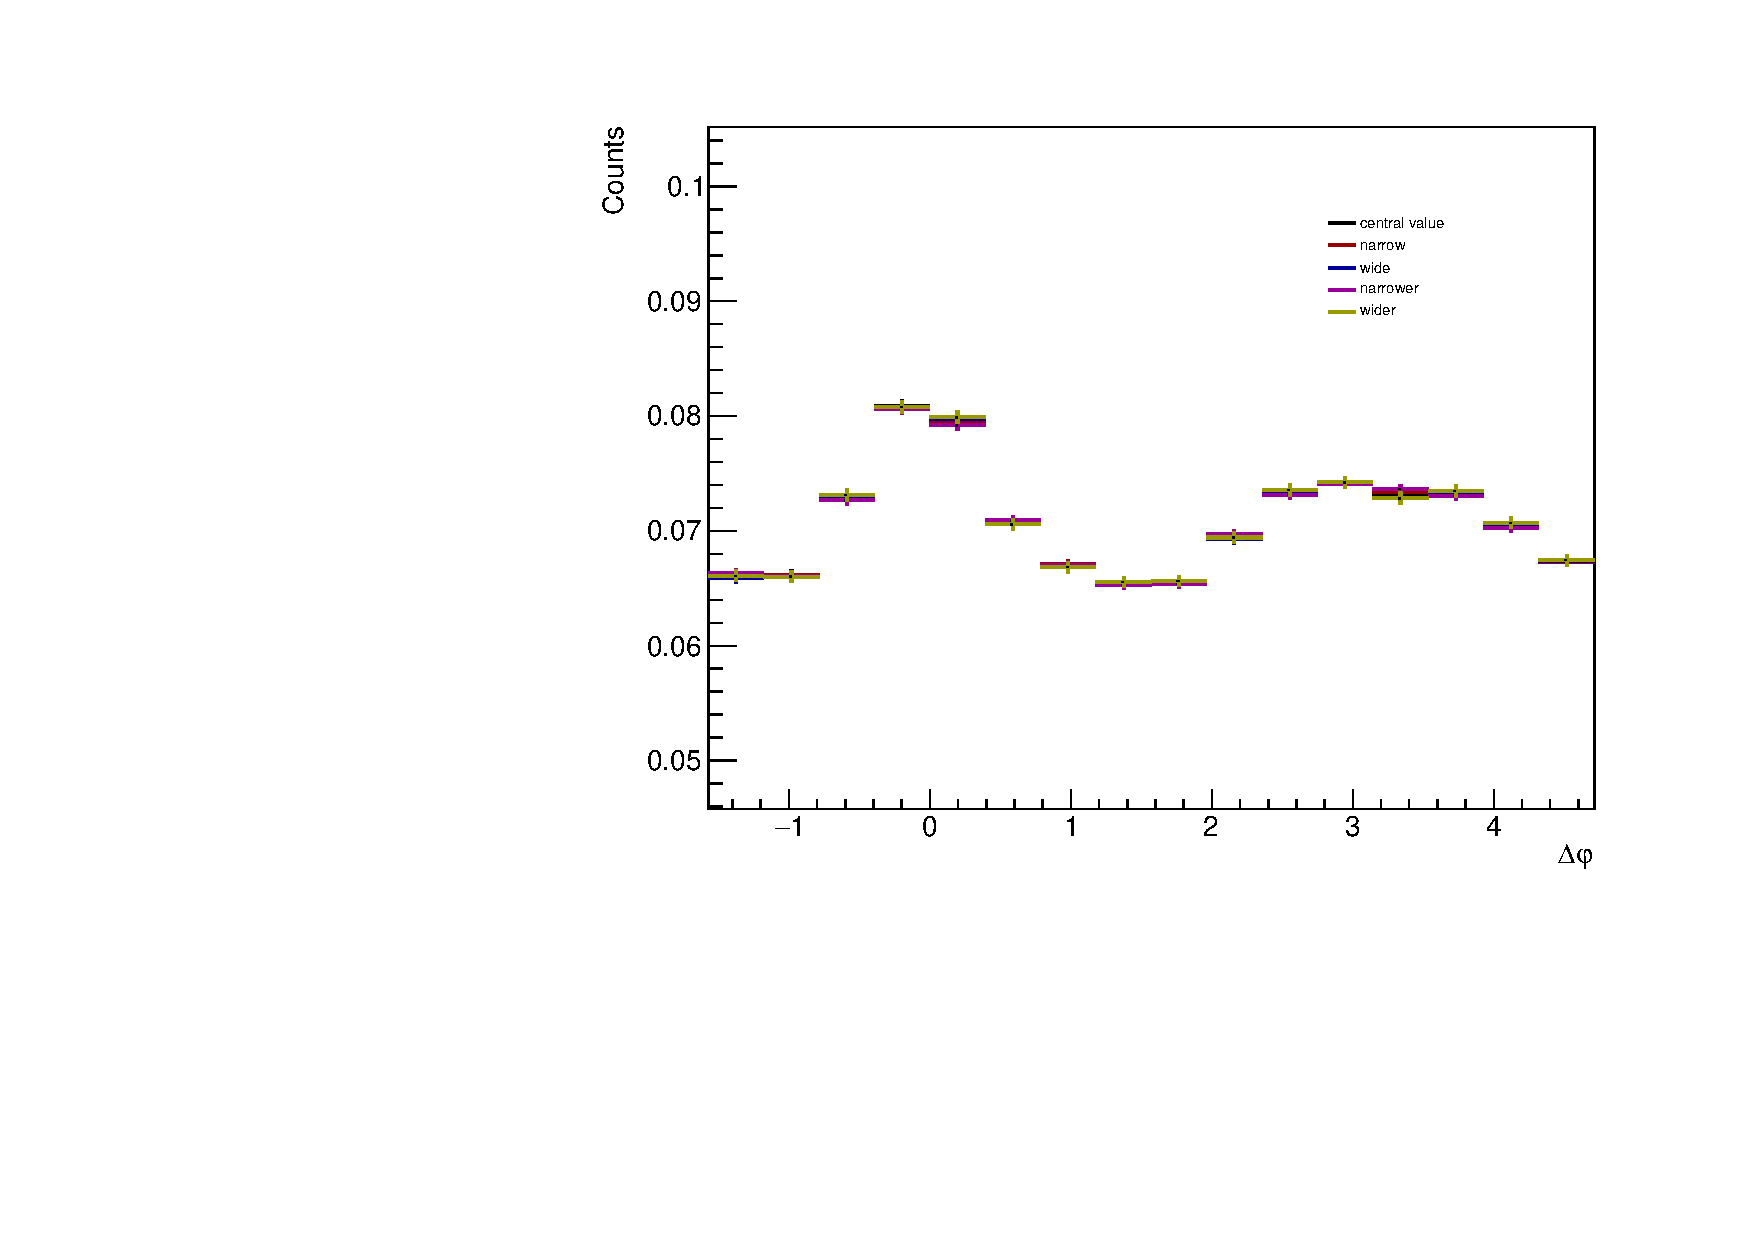
\includegraphics[width=0.49\textwidth]{figures/analysis/signal_variations_dphi_0_20_lowpt.pdf}
    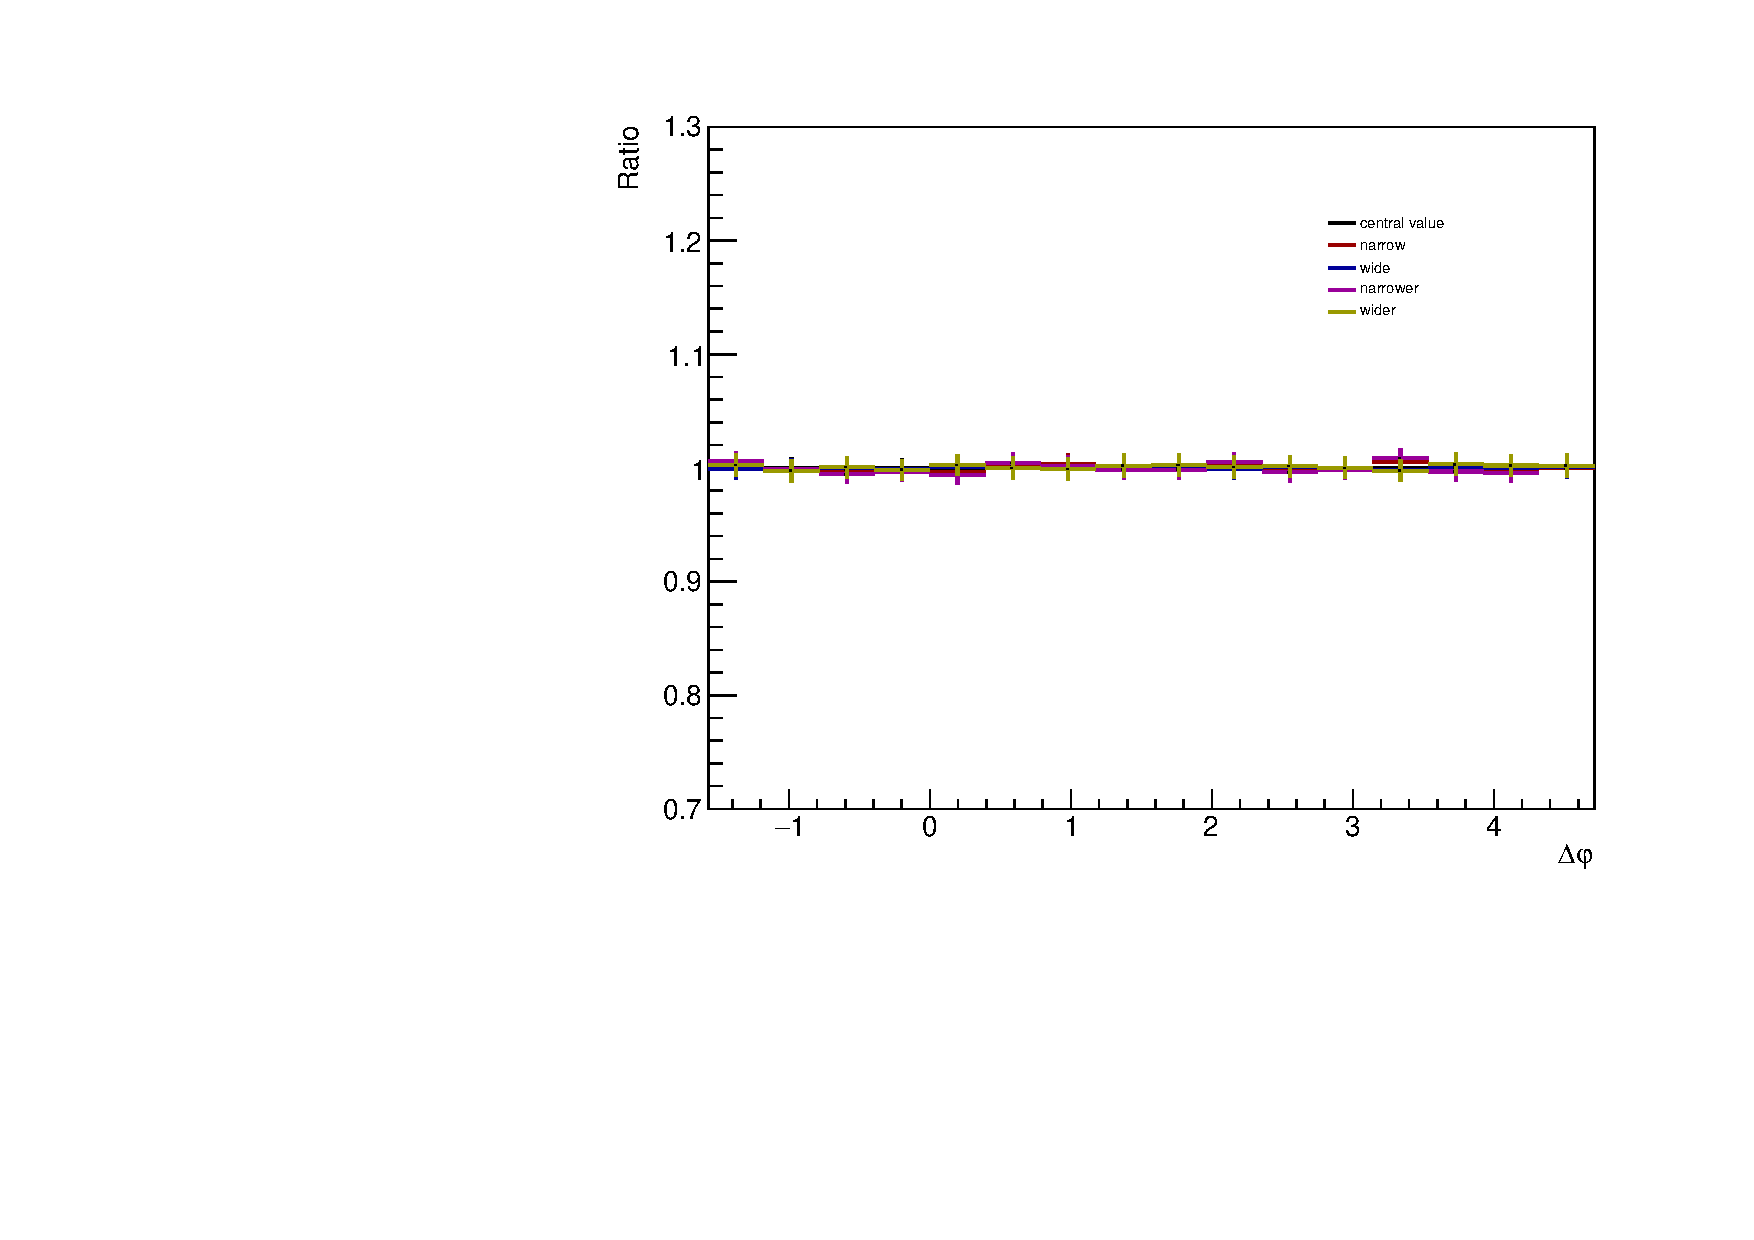
\includegraphics[width=0.49\textwidth]{figures/analysis/signal_variations_dphi_0_20_lowpt_ratio.pdf}
    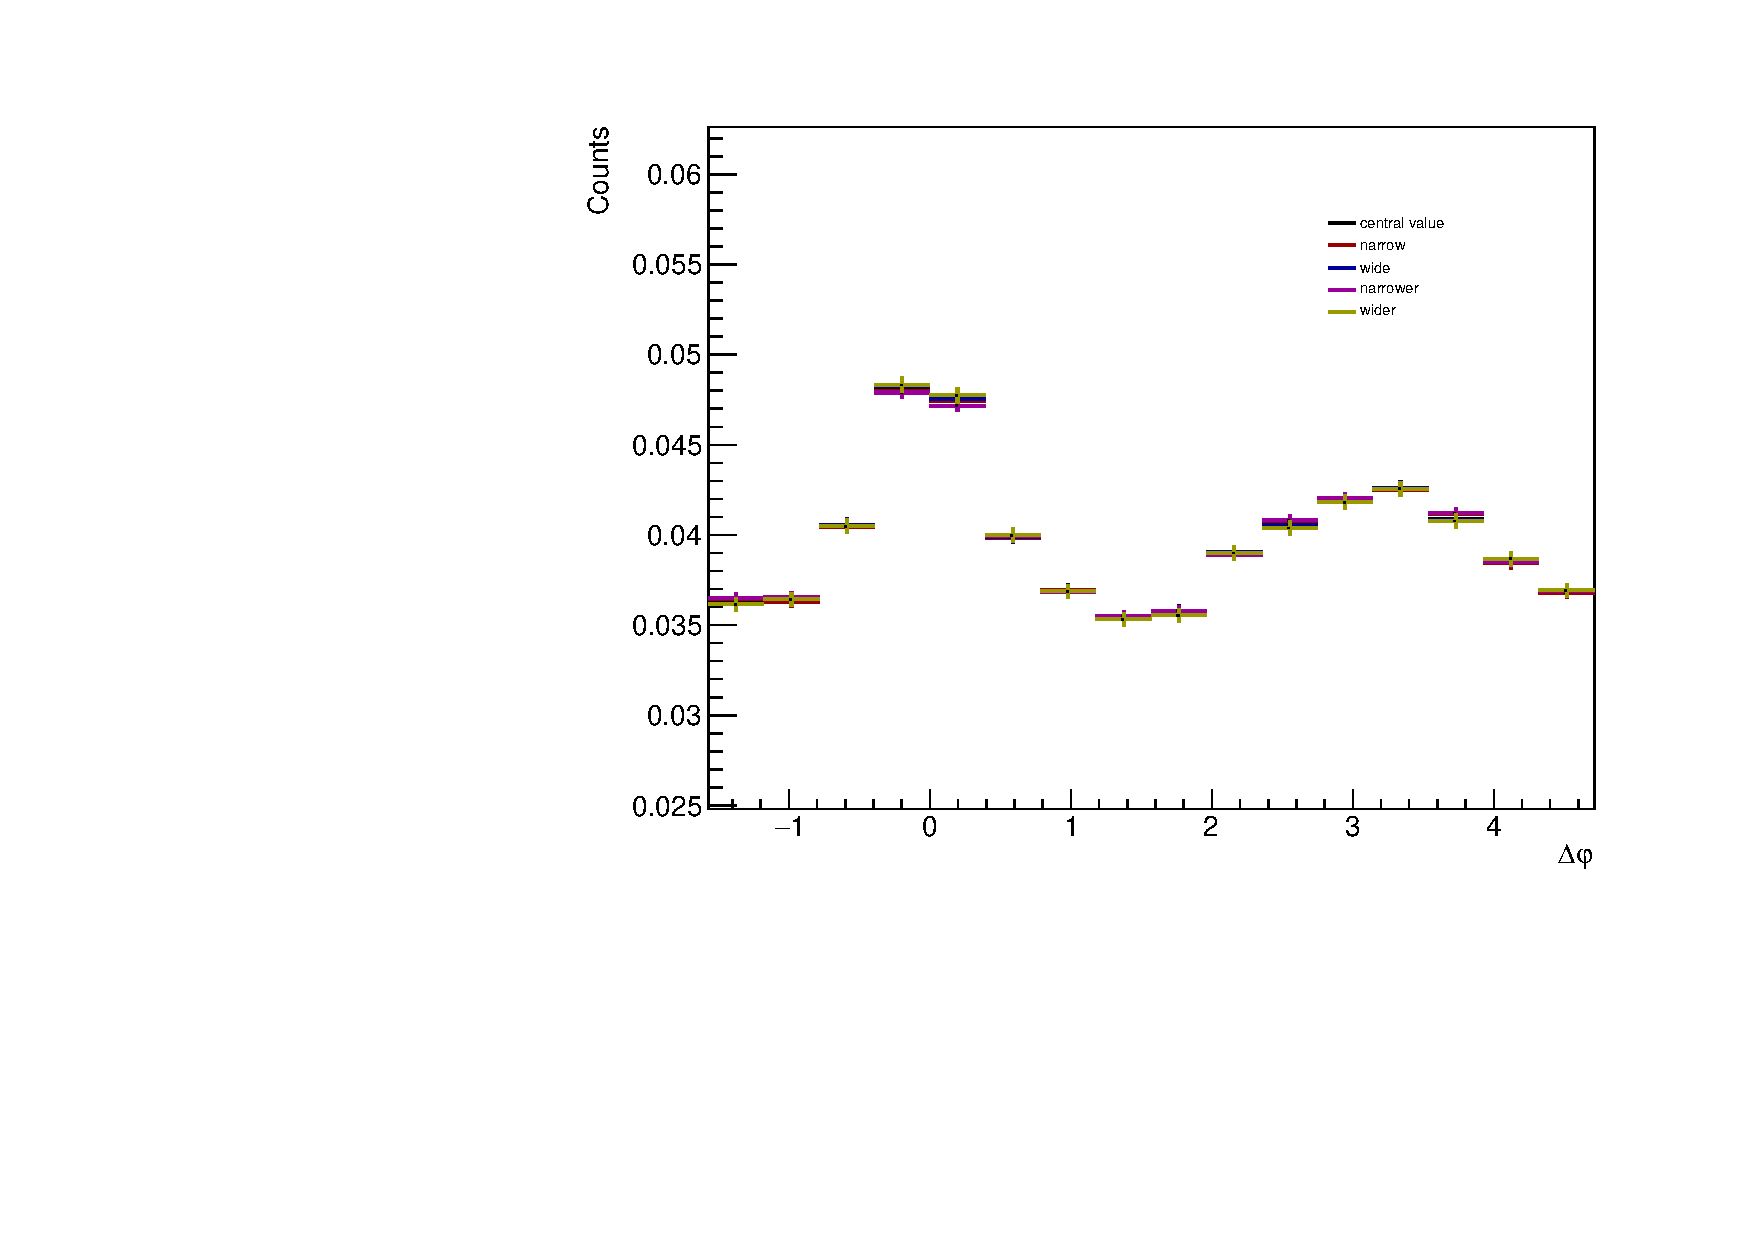
\includegraphics[width=0.49\textwidth]{figures/analysis/signal_variations_dphi_20_50_lowpt.pdf}
    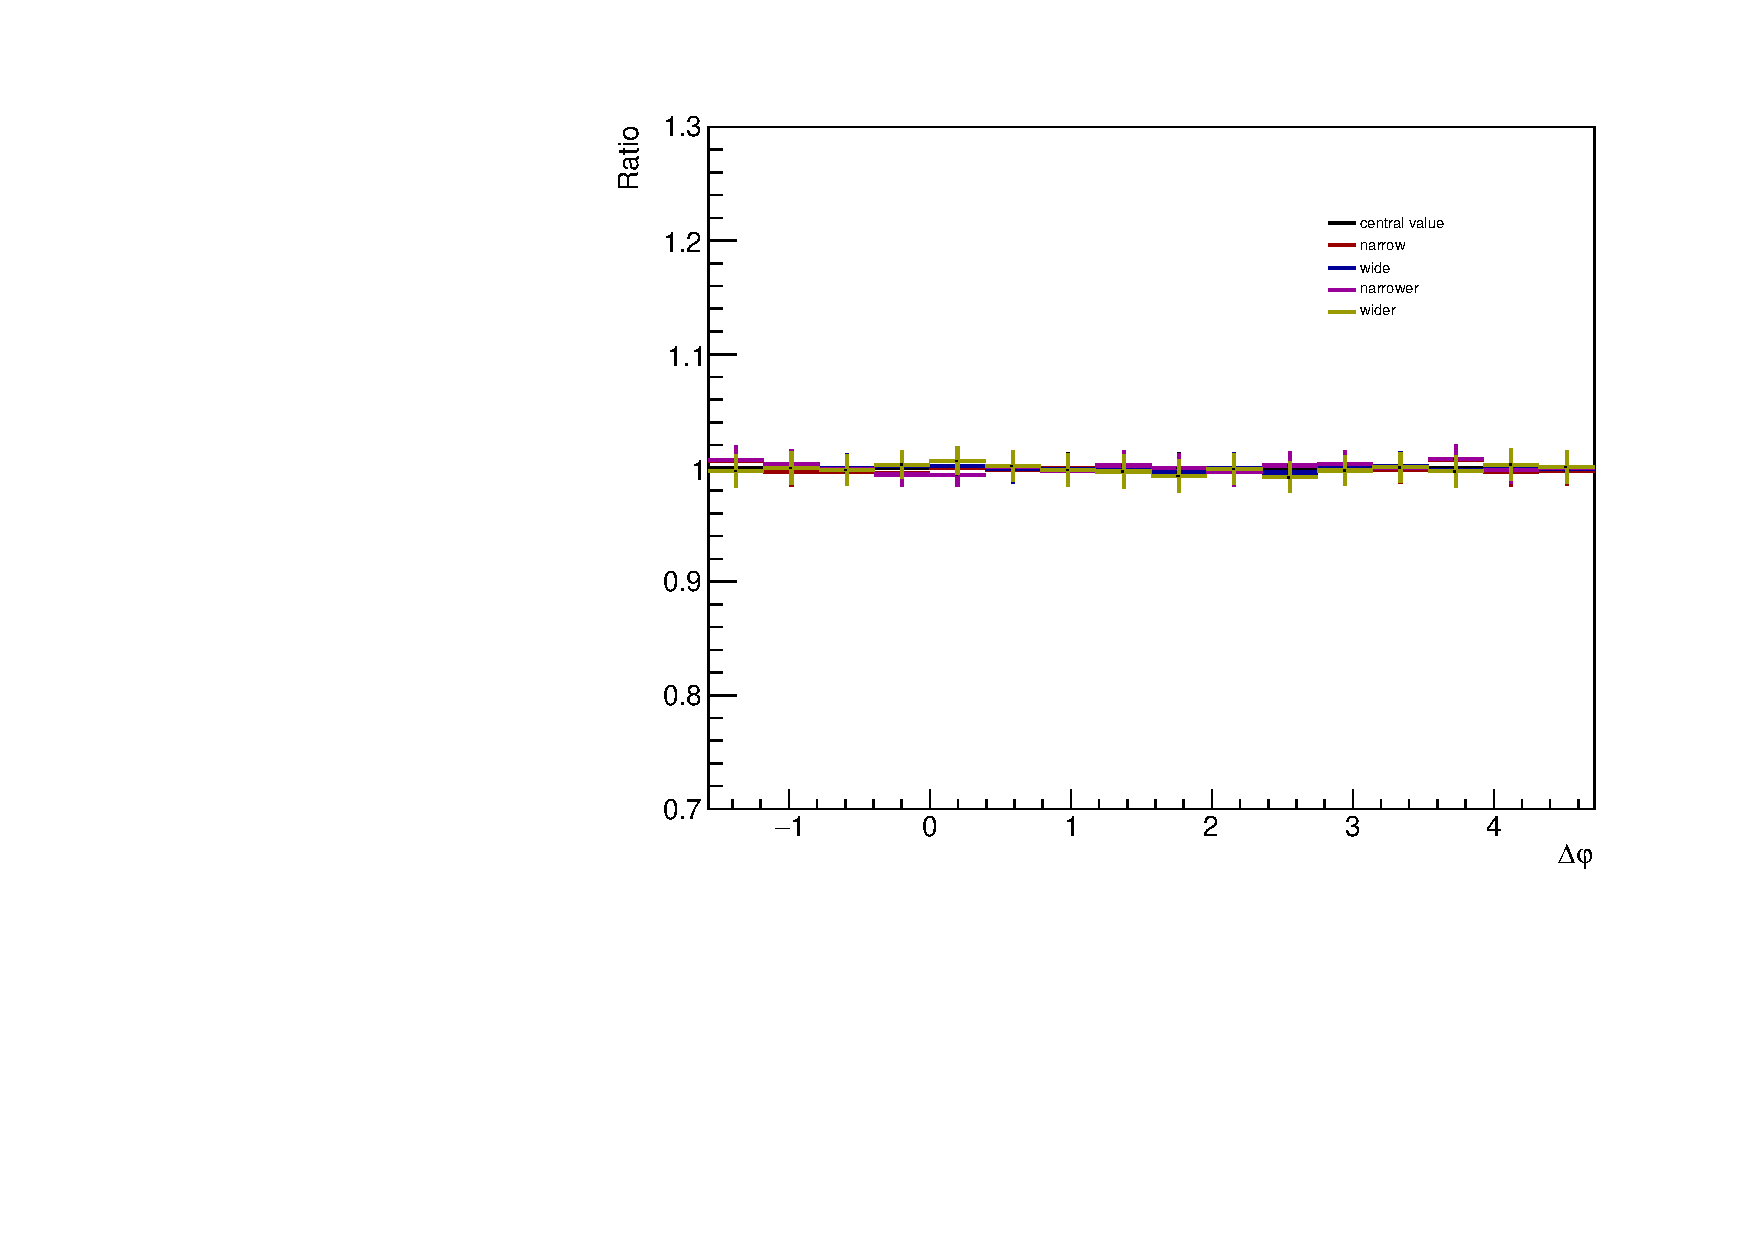
\includegraphics[width=0.49\textwidth]{figures/analysis/signal_variations_dphi_20_50_lowpt_ratio.pdf}
    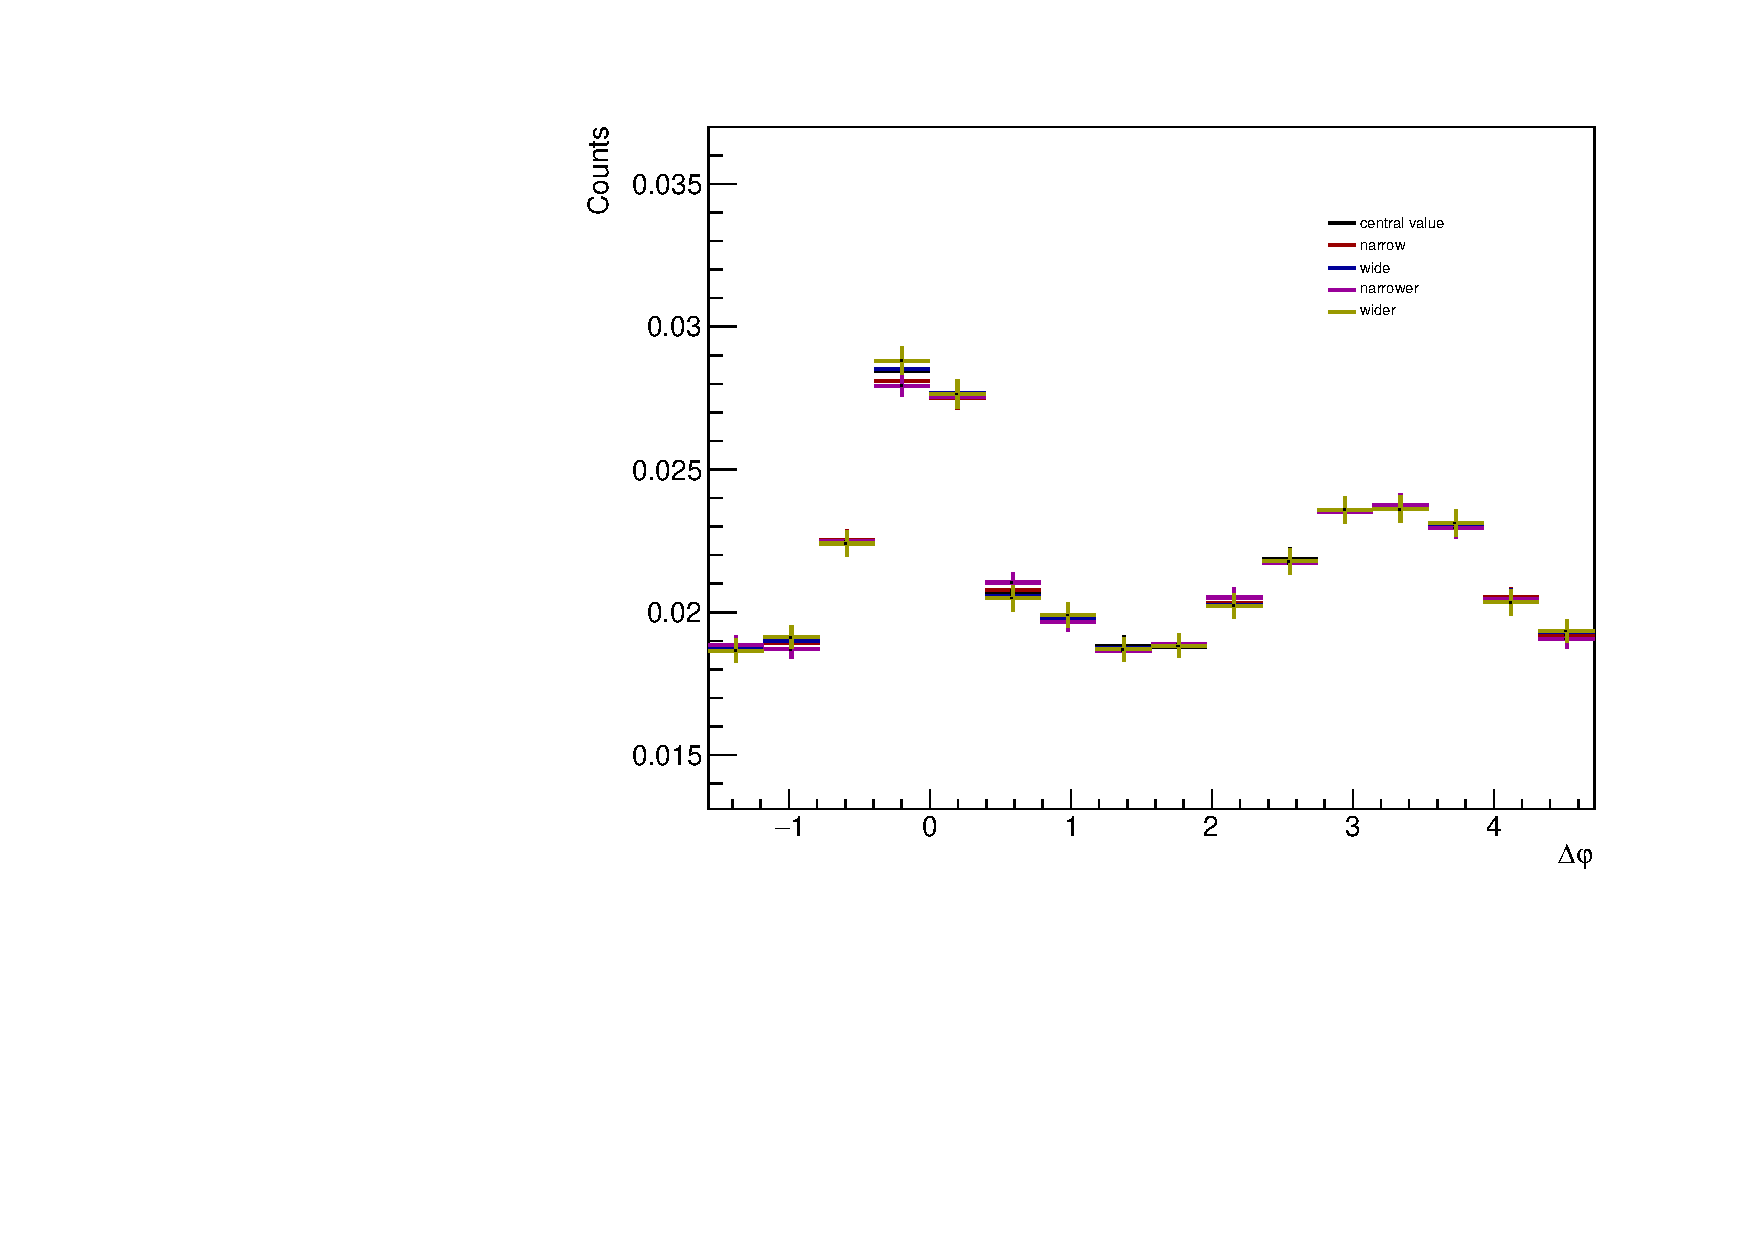
\includegraphics[width=0.49\textwidth]{figures/analysis/signal_variations_dphi_50_80_lowpt.pdf}
    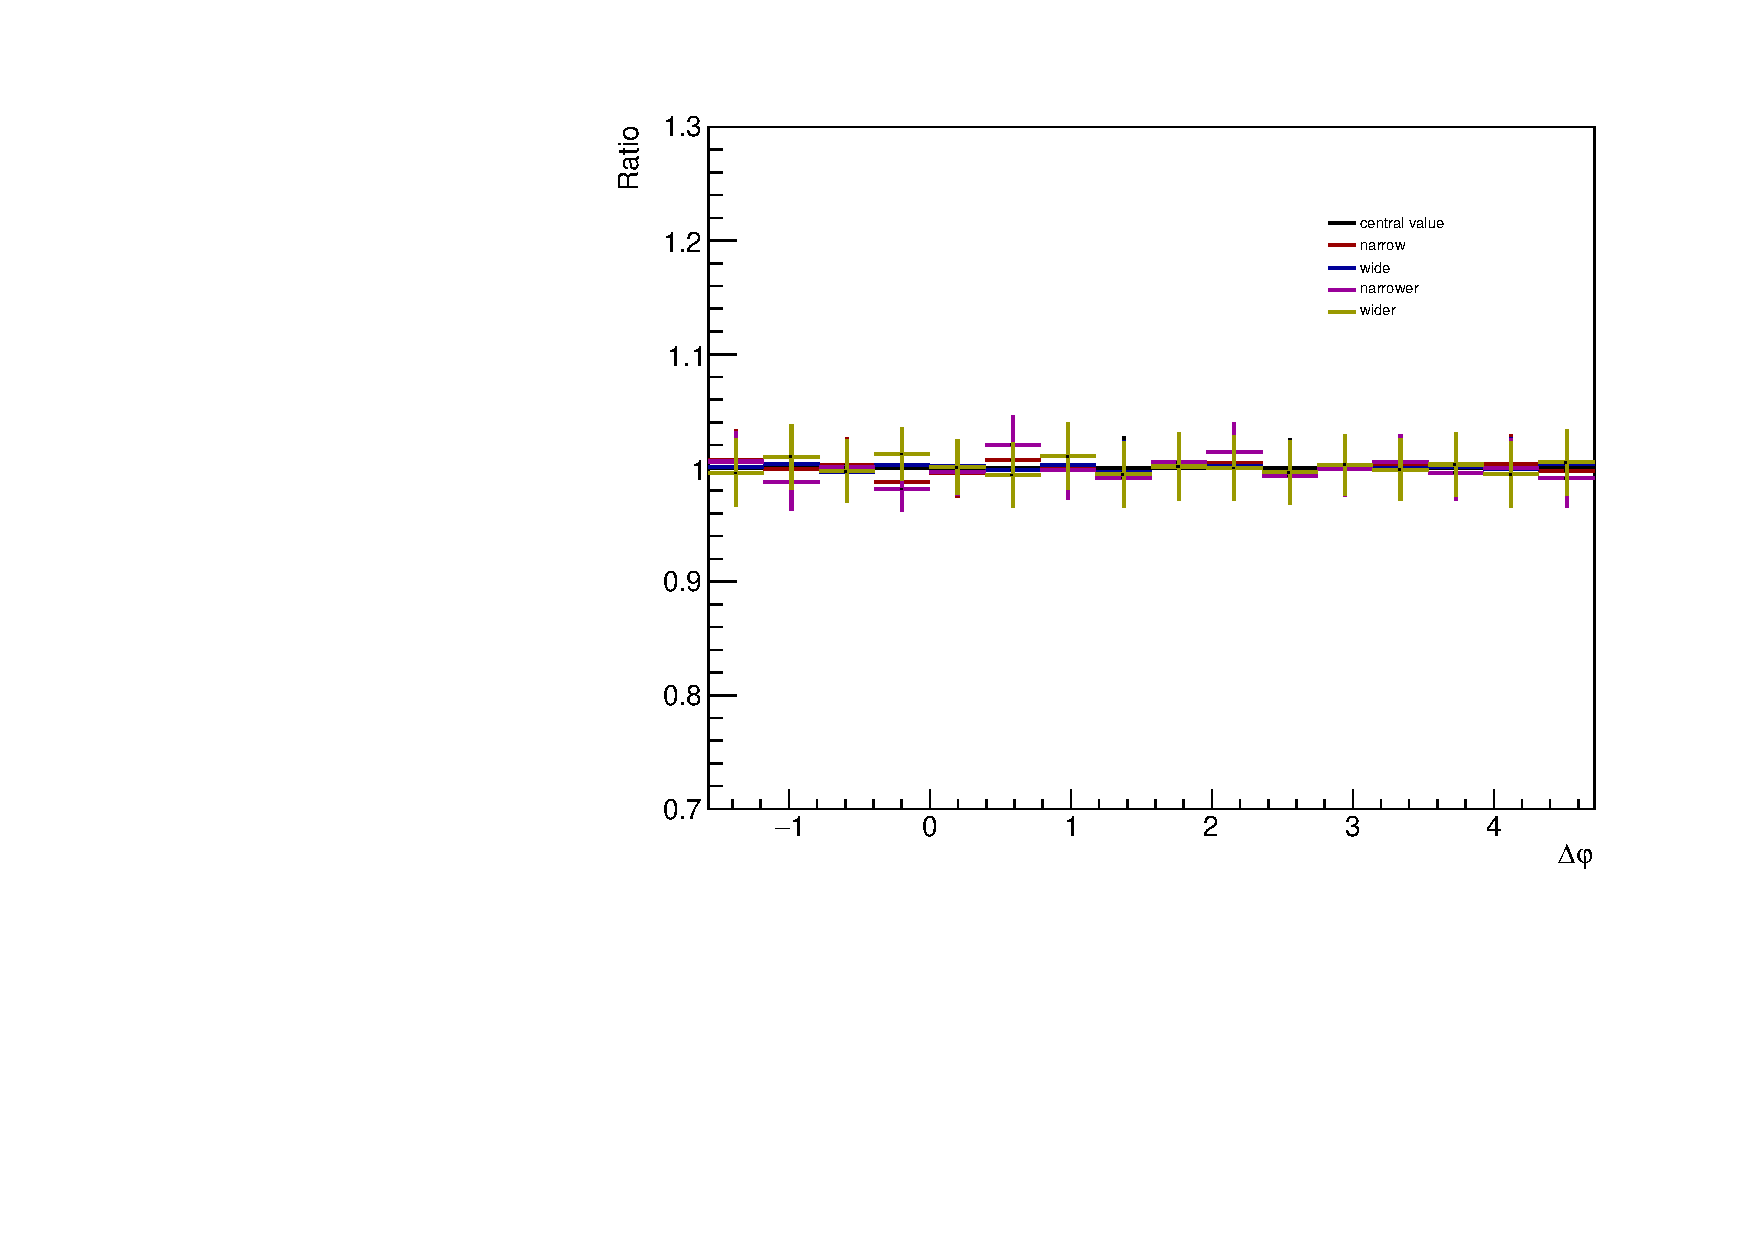
\includegraphics[width=0.49\textwidth]{figures/analysis/signal_variations_dphi_50_80_lowpt_ratio.pdf}
    \caption{The h-\lmb $\Delta\varphi$ distributions within the 0-20\% (top), 20-50\% (middle) and 50-80\% (bottom) multiplicity bins in the lower associated \pt bin for each of the signal region variations (left) with the ratios to the nominal distribution (right).}
    \label{fig:signal_region_variations_lowpt}
\end{figure}

\begin{figure}[ht]
    \centering
    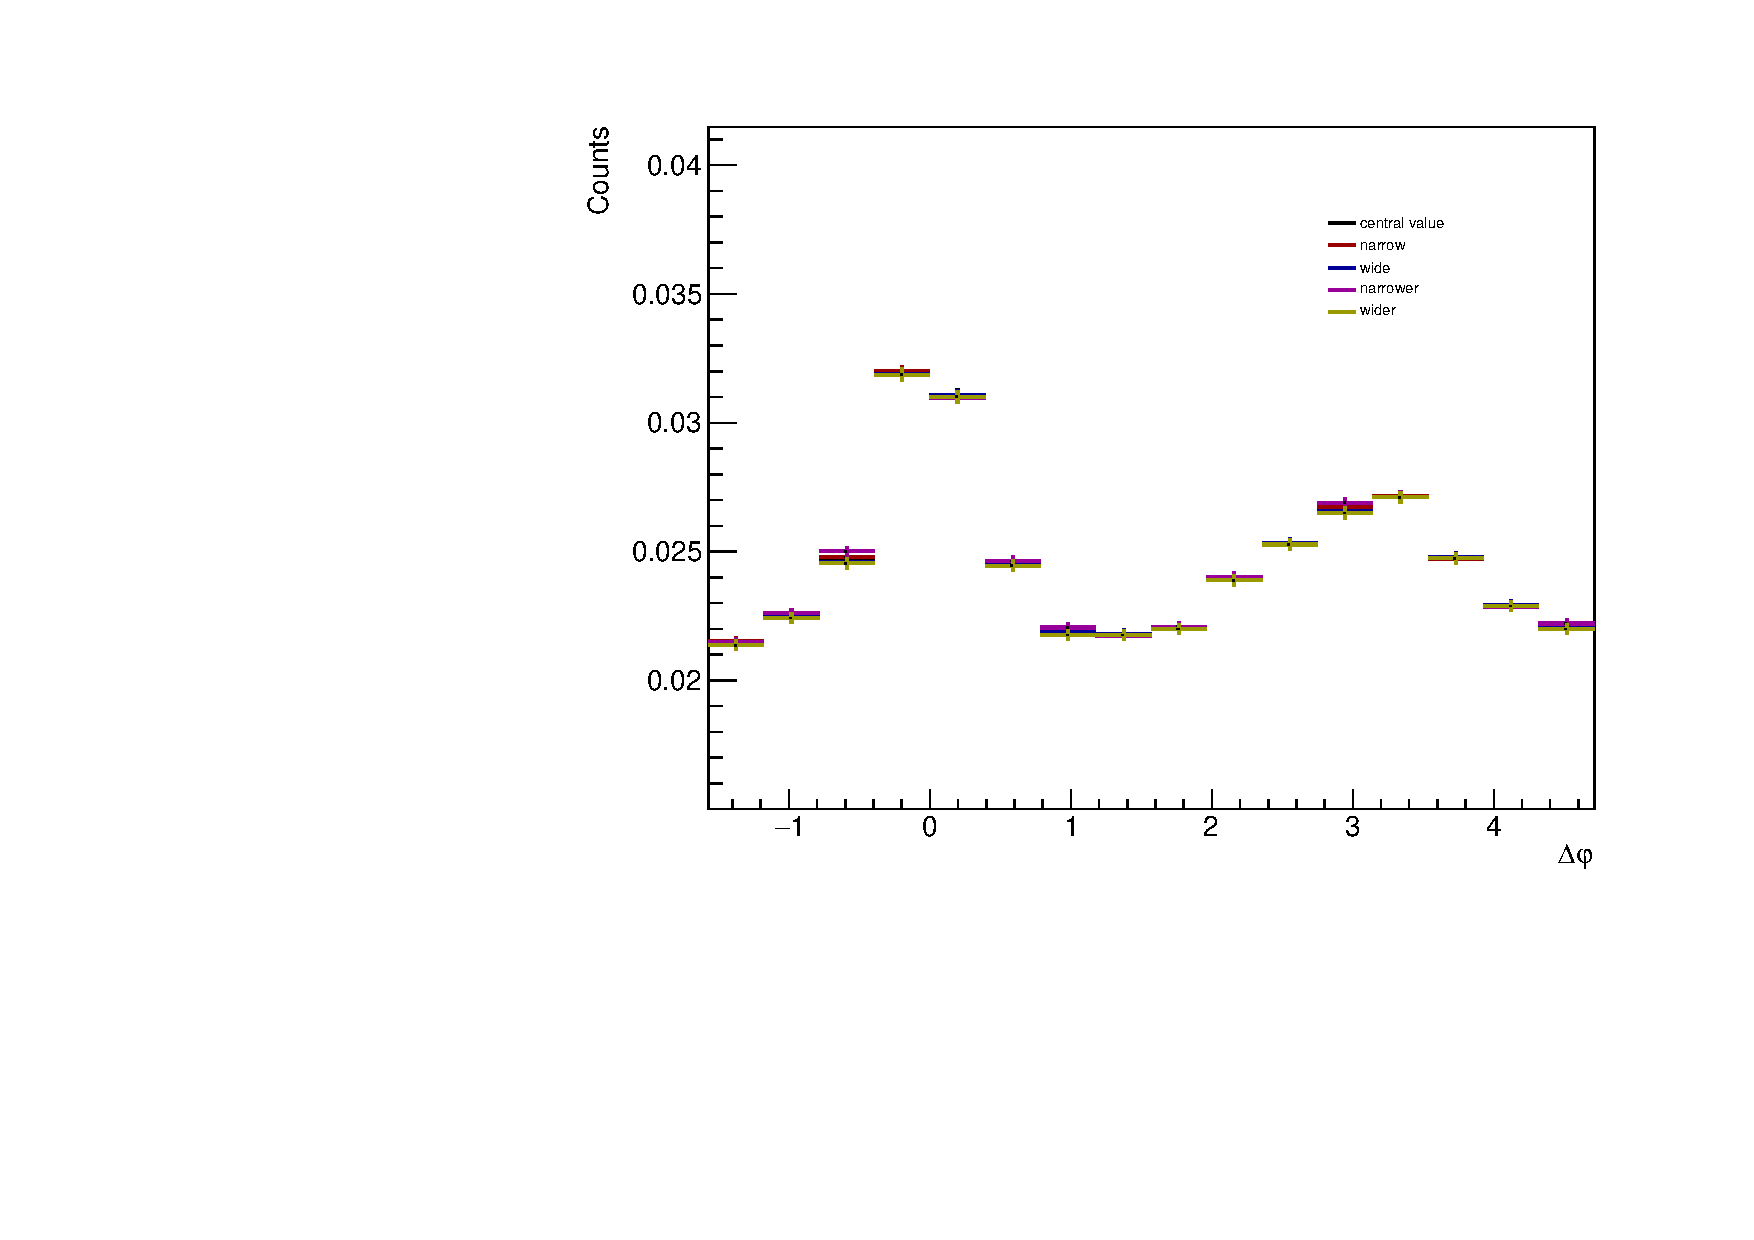
\includegraphics[width=0.49\textwidth]{figures/analysis/signal_variations_dphi_0_20_highpt.pdf}
    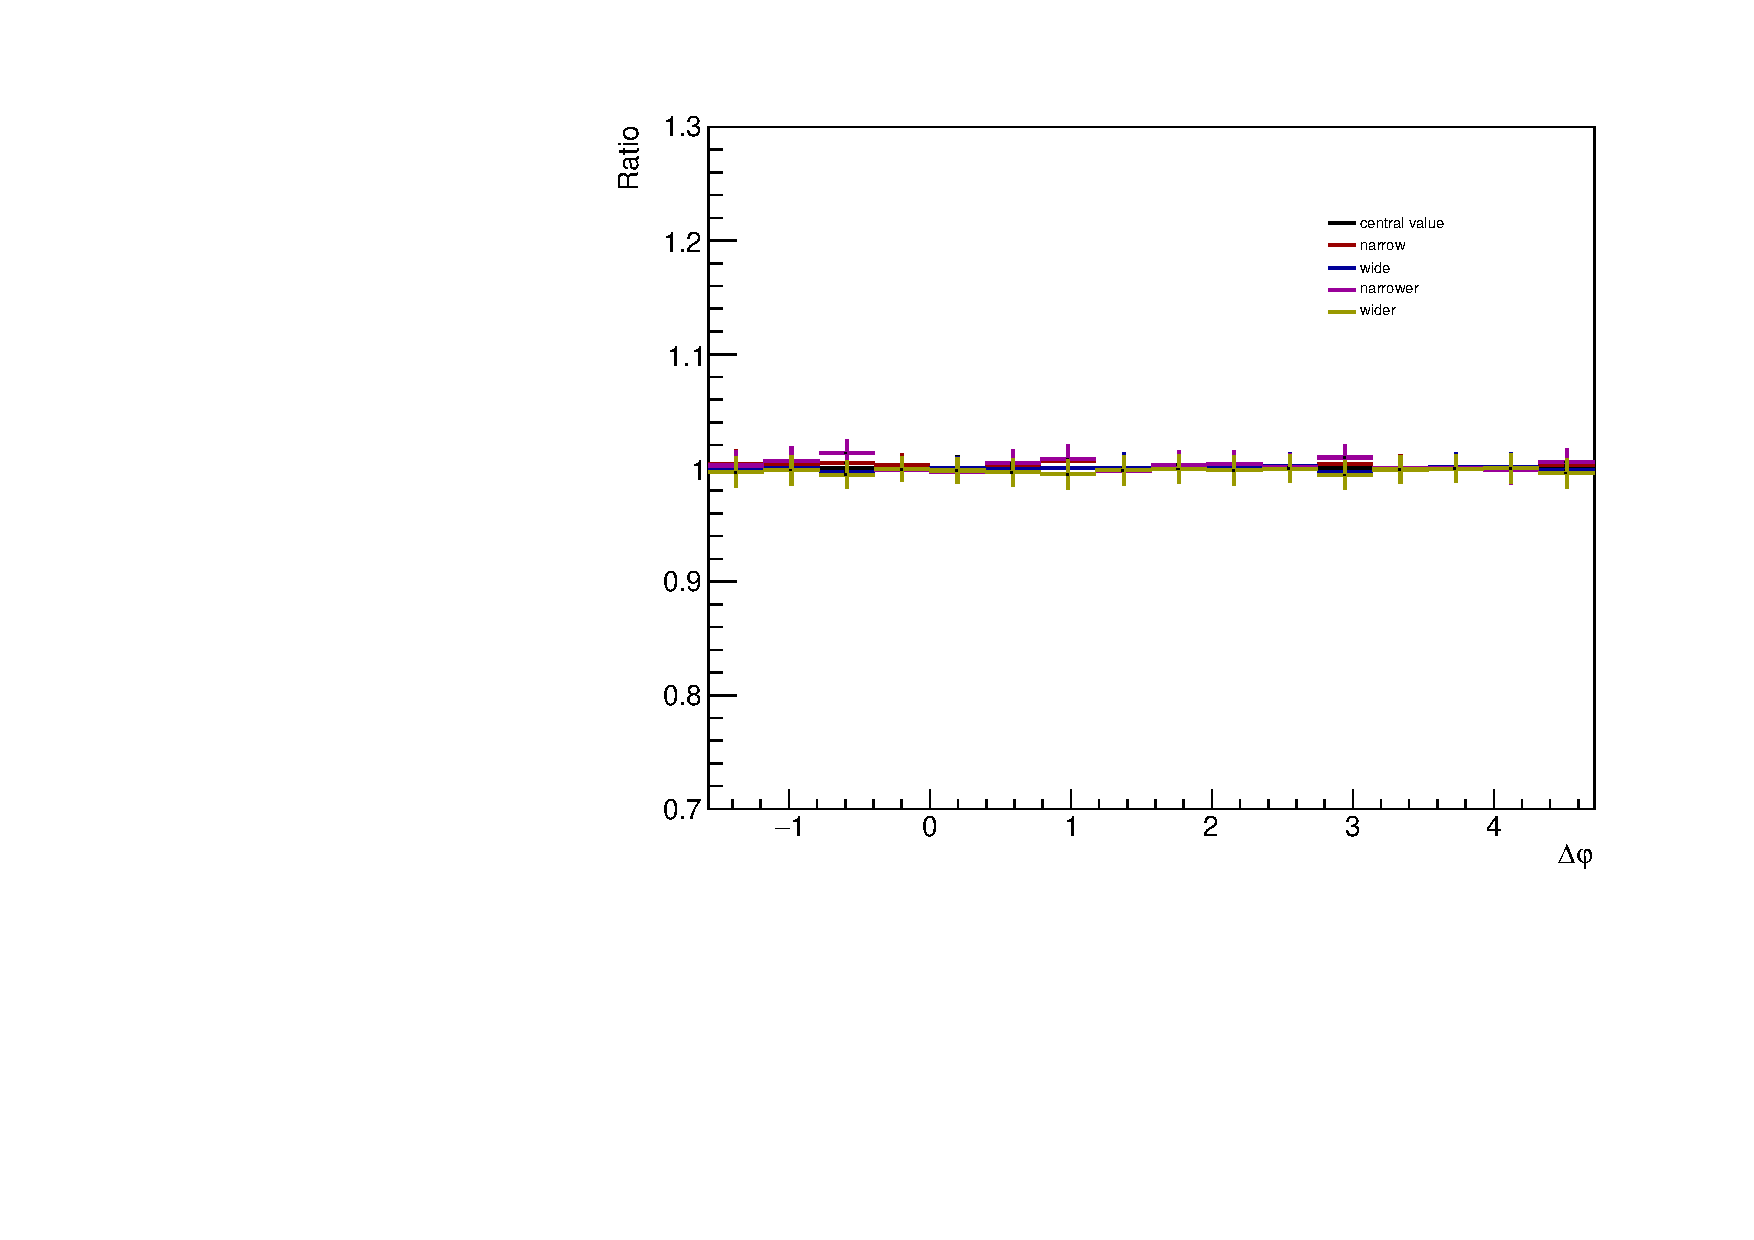
\includegraphics[width=0.49\textwidth]{figures/analysis/signal_variations_dphi_0_20_highpt_ratio.pdf}
    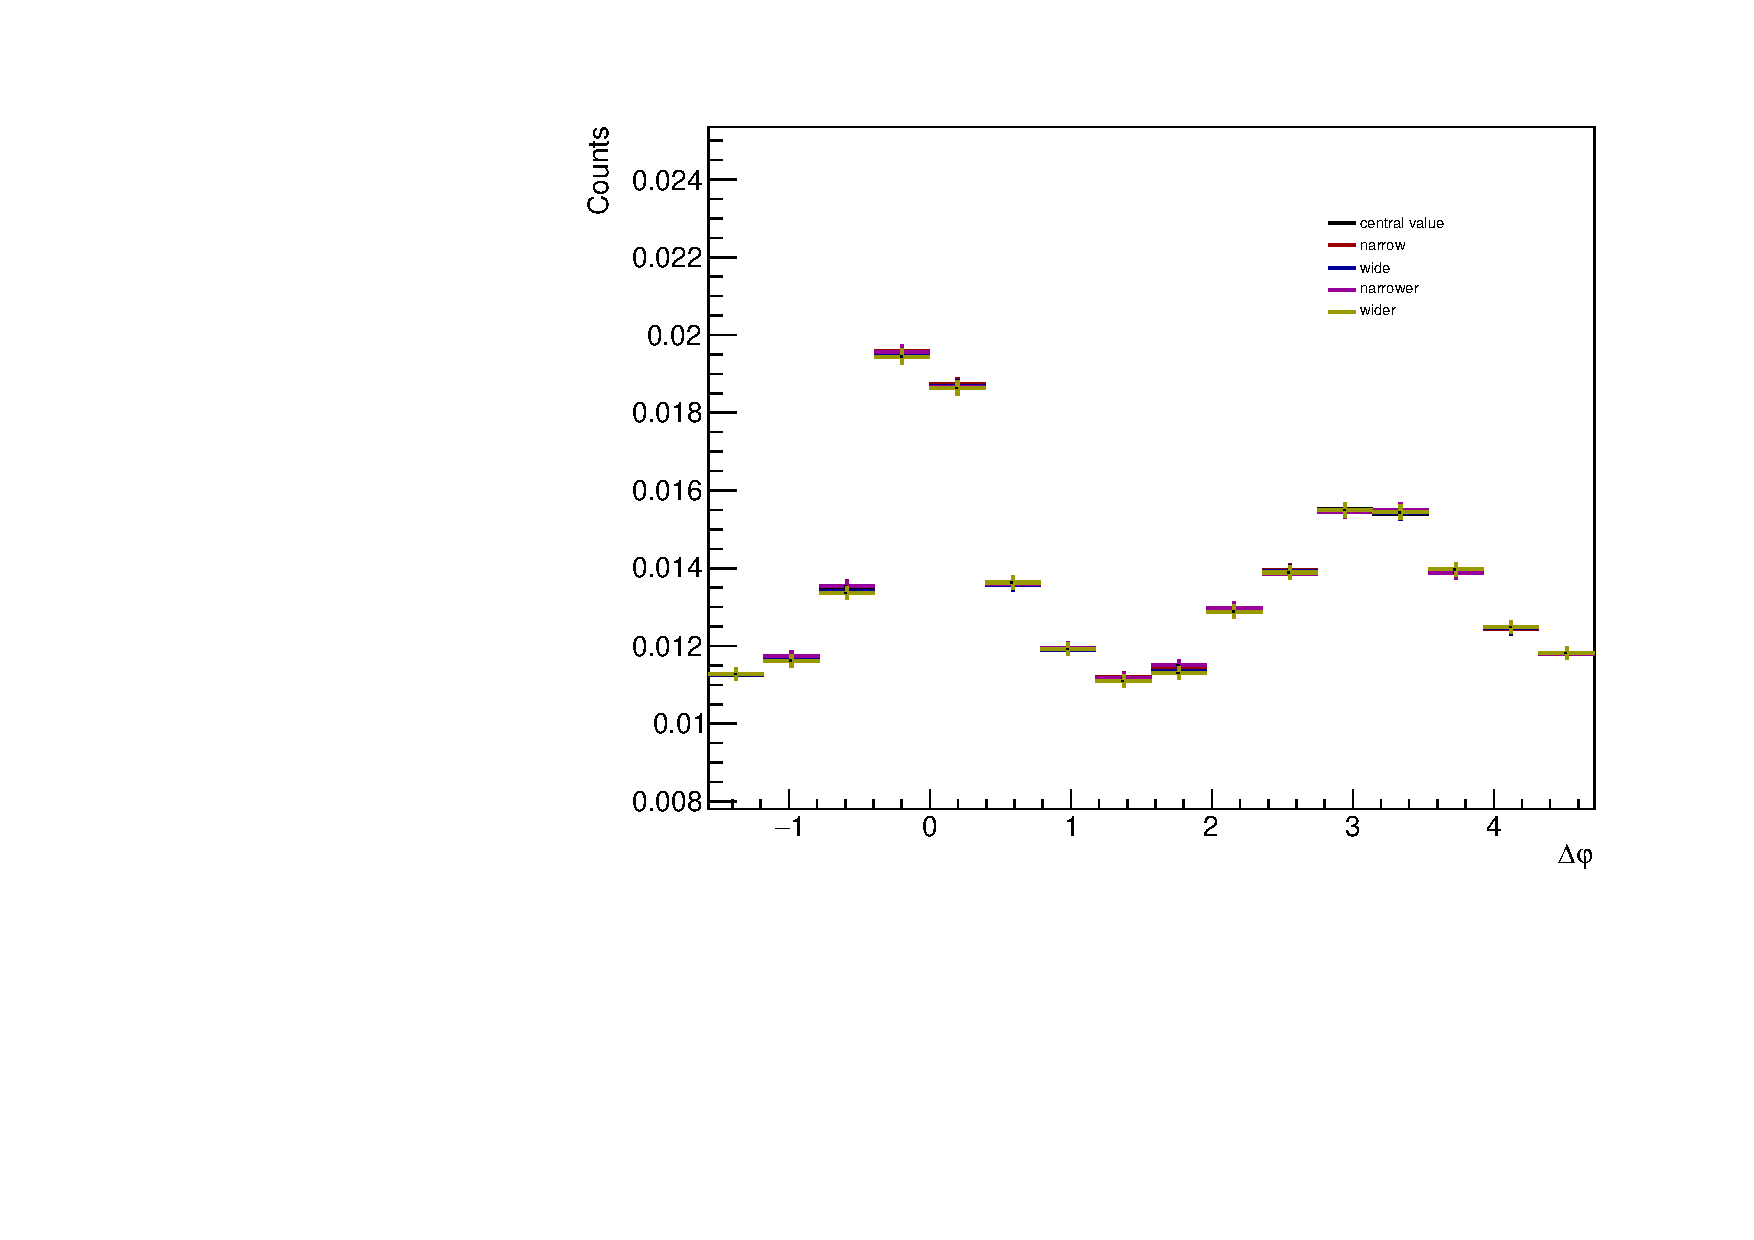
\includegraphics[width=0.49\textwidth]{figures/analysis/signal_variations_dphi_20_50_highpt.pdf}
    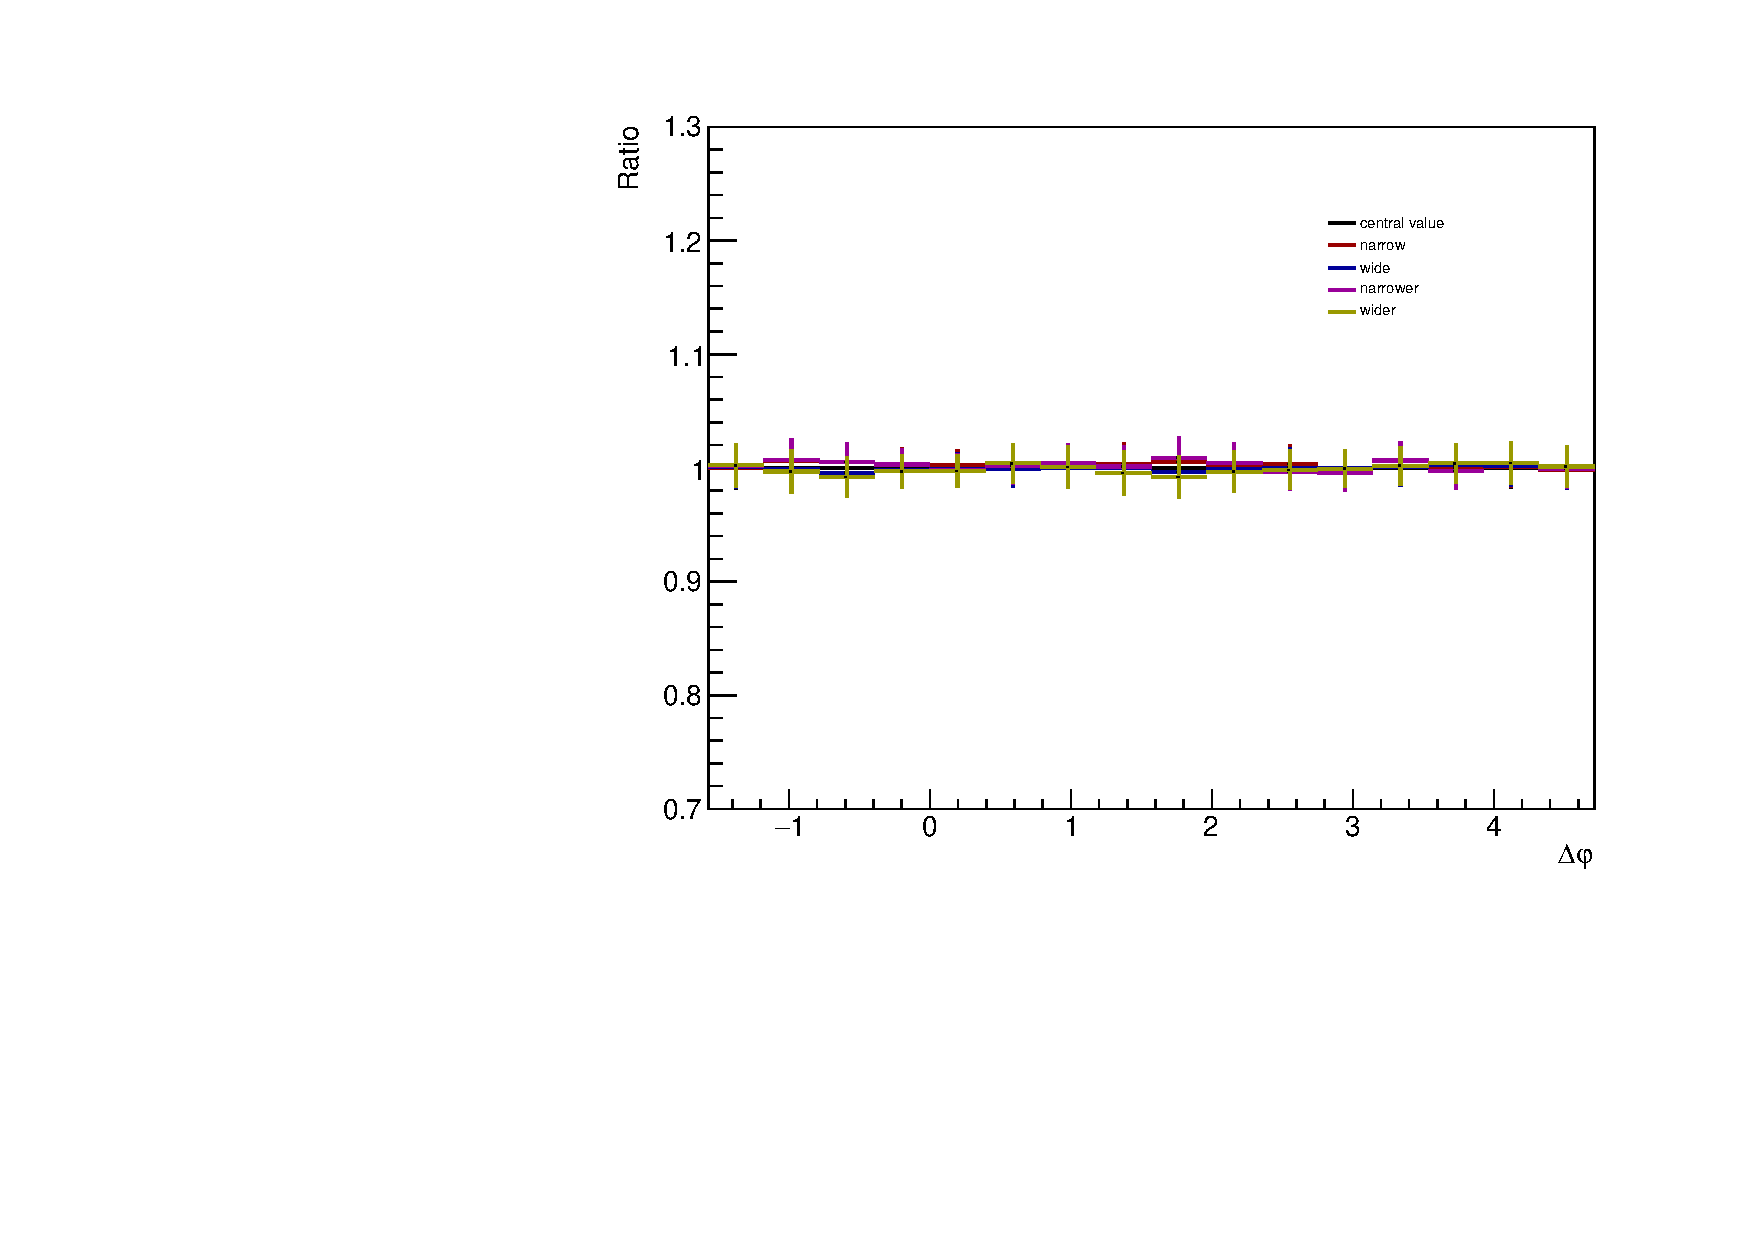
\includegraphics[width=0.49\textwidth]{figures/analysis/signal_variations_dphi_20_50_highpt_ratio.pdf}
    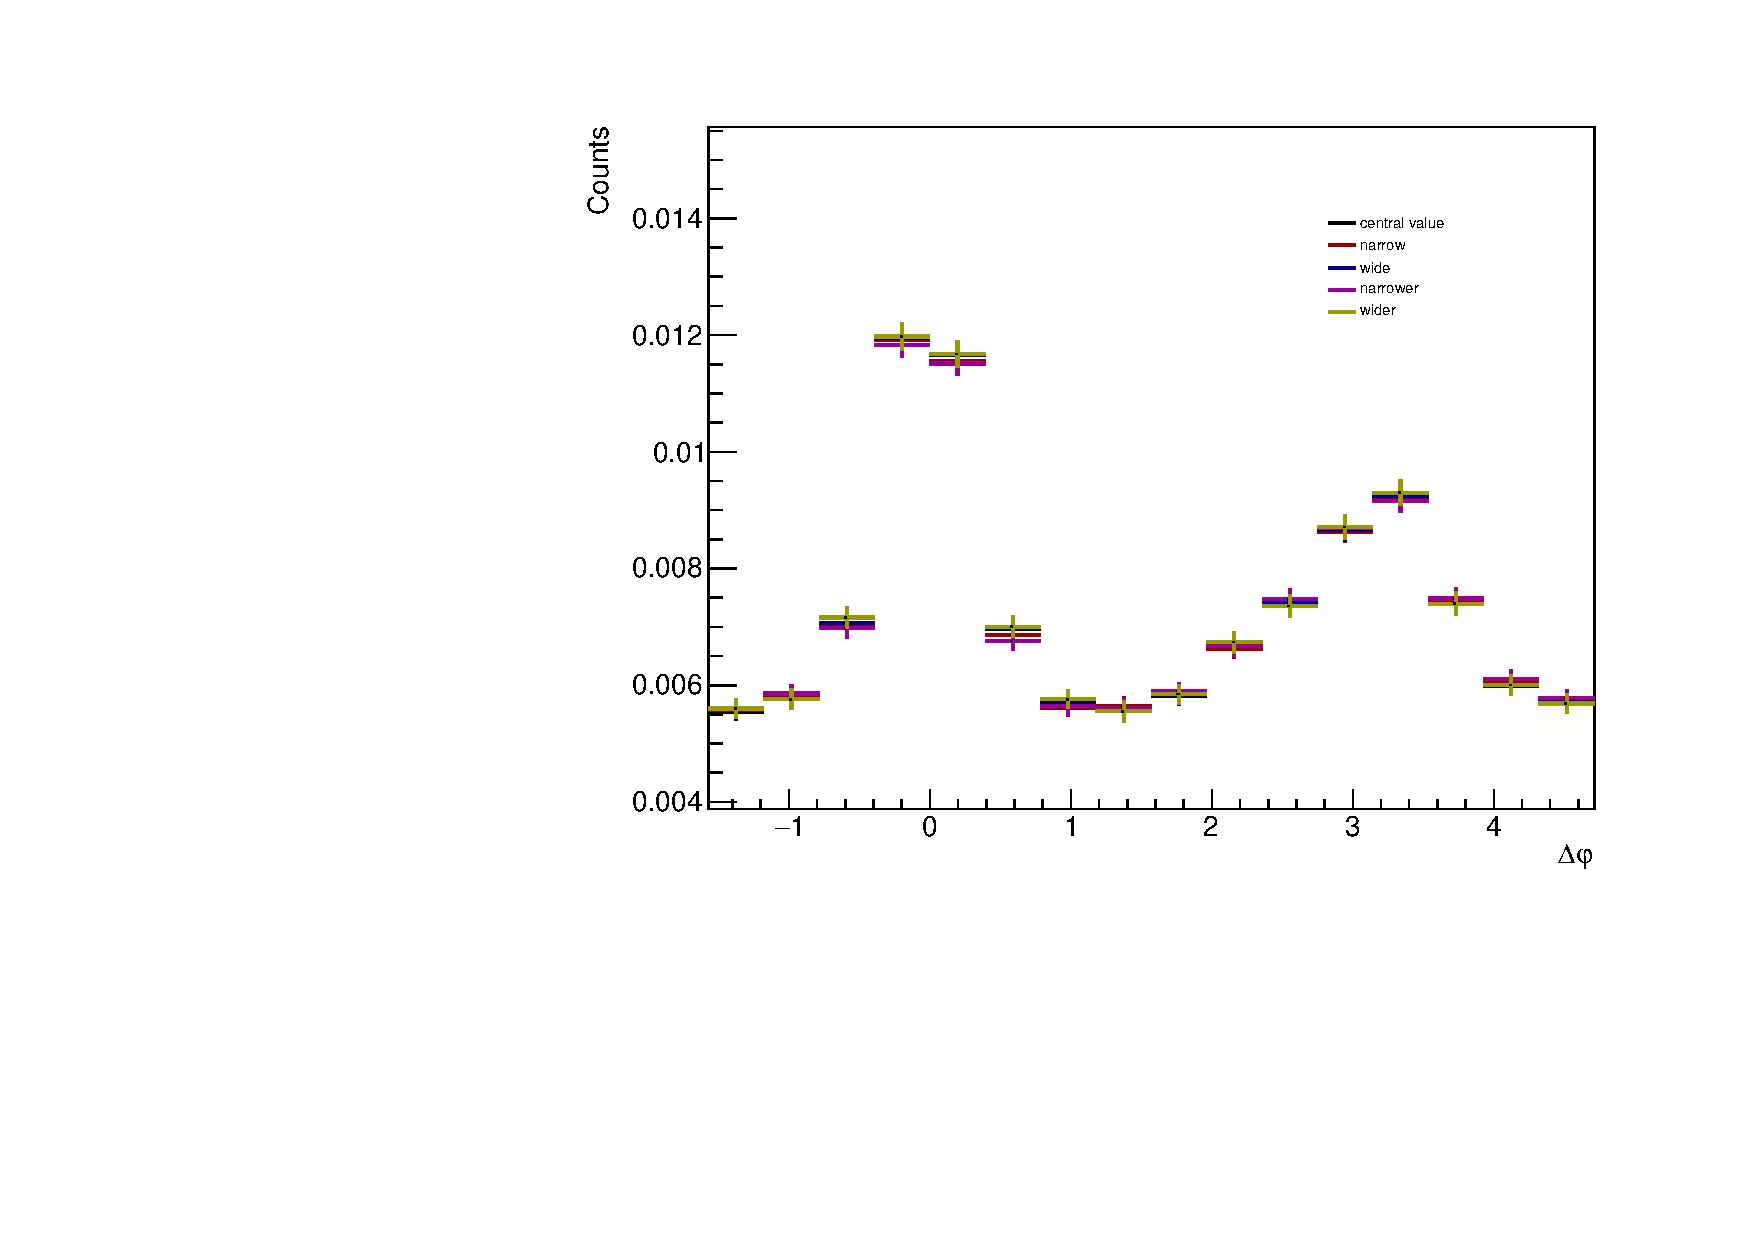
\includegraphics[width=0.49\textwidth]{figures/analysis/signal_variations_dphi_50_80_highpt.pdf}
    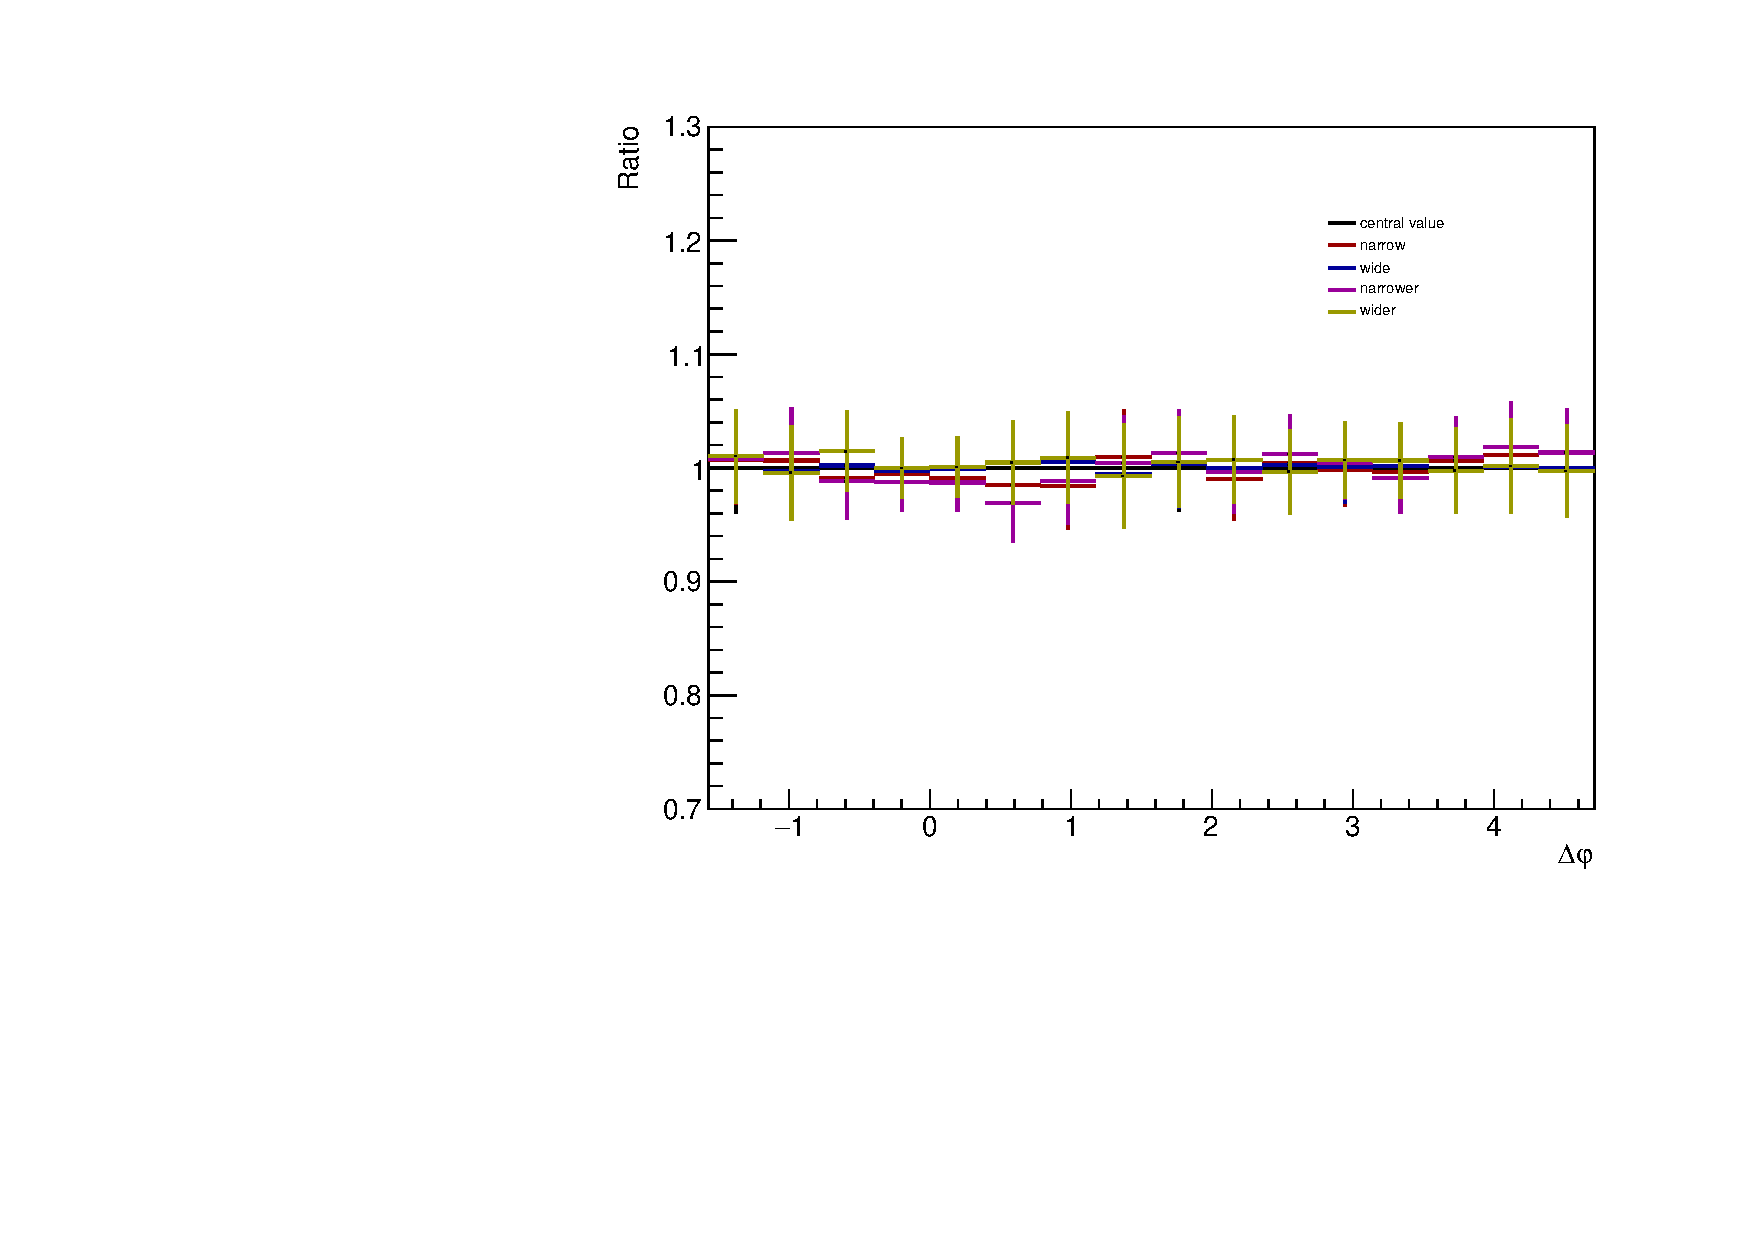
\includegraphics[width=0.49\textwidth]{figures/analysis/signal_variations_dphi_50_80_highpt_ratio.pdf}
    \caption{The h-\lmb $\Delta\varphi$ distributions within the 0-20\% (top), 20-50\% (middle) and 50-80\% (bottom) multiplicity bins in the higher associated \pt bin for each of the signal region variations (left) with the ratios to the nominal distribution (right).}
    \label{fig:signal_region_variations_highpt}
\end{figure}

\subsubsection{Sideband region selection}
The choice of sideband region also leaves a lot of room for reasonable variation: all that is required is that the region is 1) large enough to produce a smooth h-p$\pi$ distribution with minimal statisical fluctuations and 2) close enough to the signal region that the p$\pi$ pairs are kinematically similar to those in the background of the signal region. As long as these requirements are met, the final result should not be very dependent on the choice of sideband region. To investigate the effects of changing the sideband region, the variations presented in Table~\ref{tab:sideband_region_variations} are considered. The measured $\Delta\varphi$ distributions and variation/nominal ratios for each sideband region variation in each multiplicity and associated \pt bin are shown in Figures \ref{fig:sideband_region_variations_lowpt} (lower \pt) and \ref{fig:sideband_region_variations_highpt} (higher \pt). The result is even less deviation from the nominal distribution than the signal region variations, with the average deviation being closer to ~1\%. Again, no significant dependence is observed on $\Delta\varphi$, so the systematic uncertainty is calculated as the RMS of the percent change from each variation across every $\Delta\varphi$ bin.

\begin{table}[ht]
    \centering
    \caption{The variations of the \lmb invariant mass sideband region considered for this analysis. Note that the ``shifted left'' sideband falls on the opposite (left) side of the signal region.}
    \label{tab:sideband_region_variations}
    \begin{tabular}{l c}
        \hline
        Variation name & Sideband range (GeV/$c^2$) \\
        \hline
        Narrow & $1.135 < M_{p\pi} < 1.145$ \\
        Wide & $1.135 < M_{p\pi} < 1.16$ \\
        Shifted left & $1.086 < M_{p\pi} < 1.098$ \\
        Shifted right & $1.14 < M_{p\pi} < 1.155$ \\
        \hline
    \end{tabular}
\end{table}

\begin{figure}[ht]
    \centering
    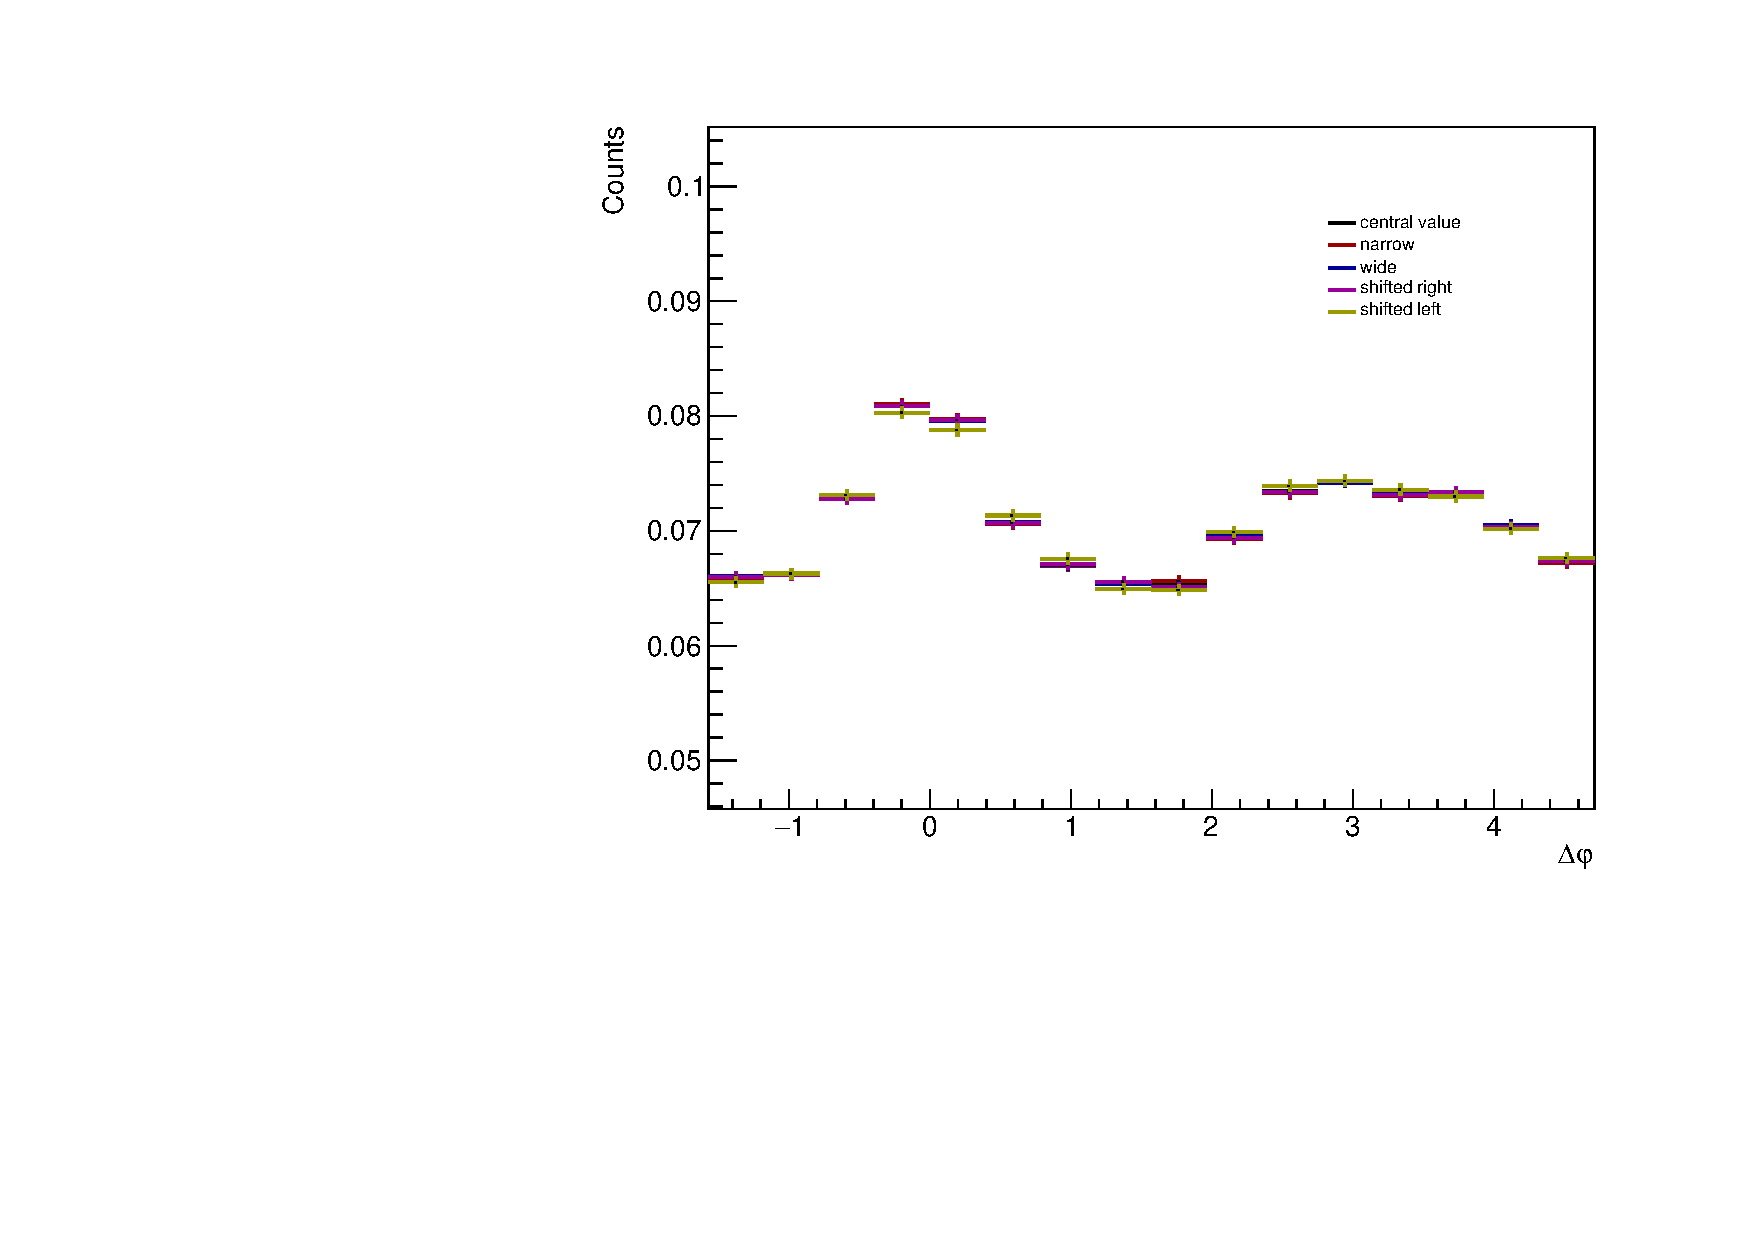
\includegraphics[width=0.49\textwidth]{figures/analysis/sideband_variations_dphi_0_20_lowpt.pdf}
    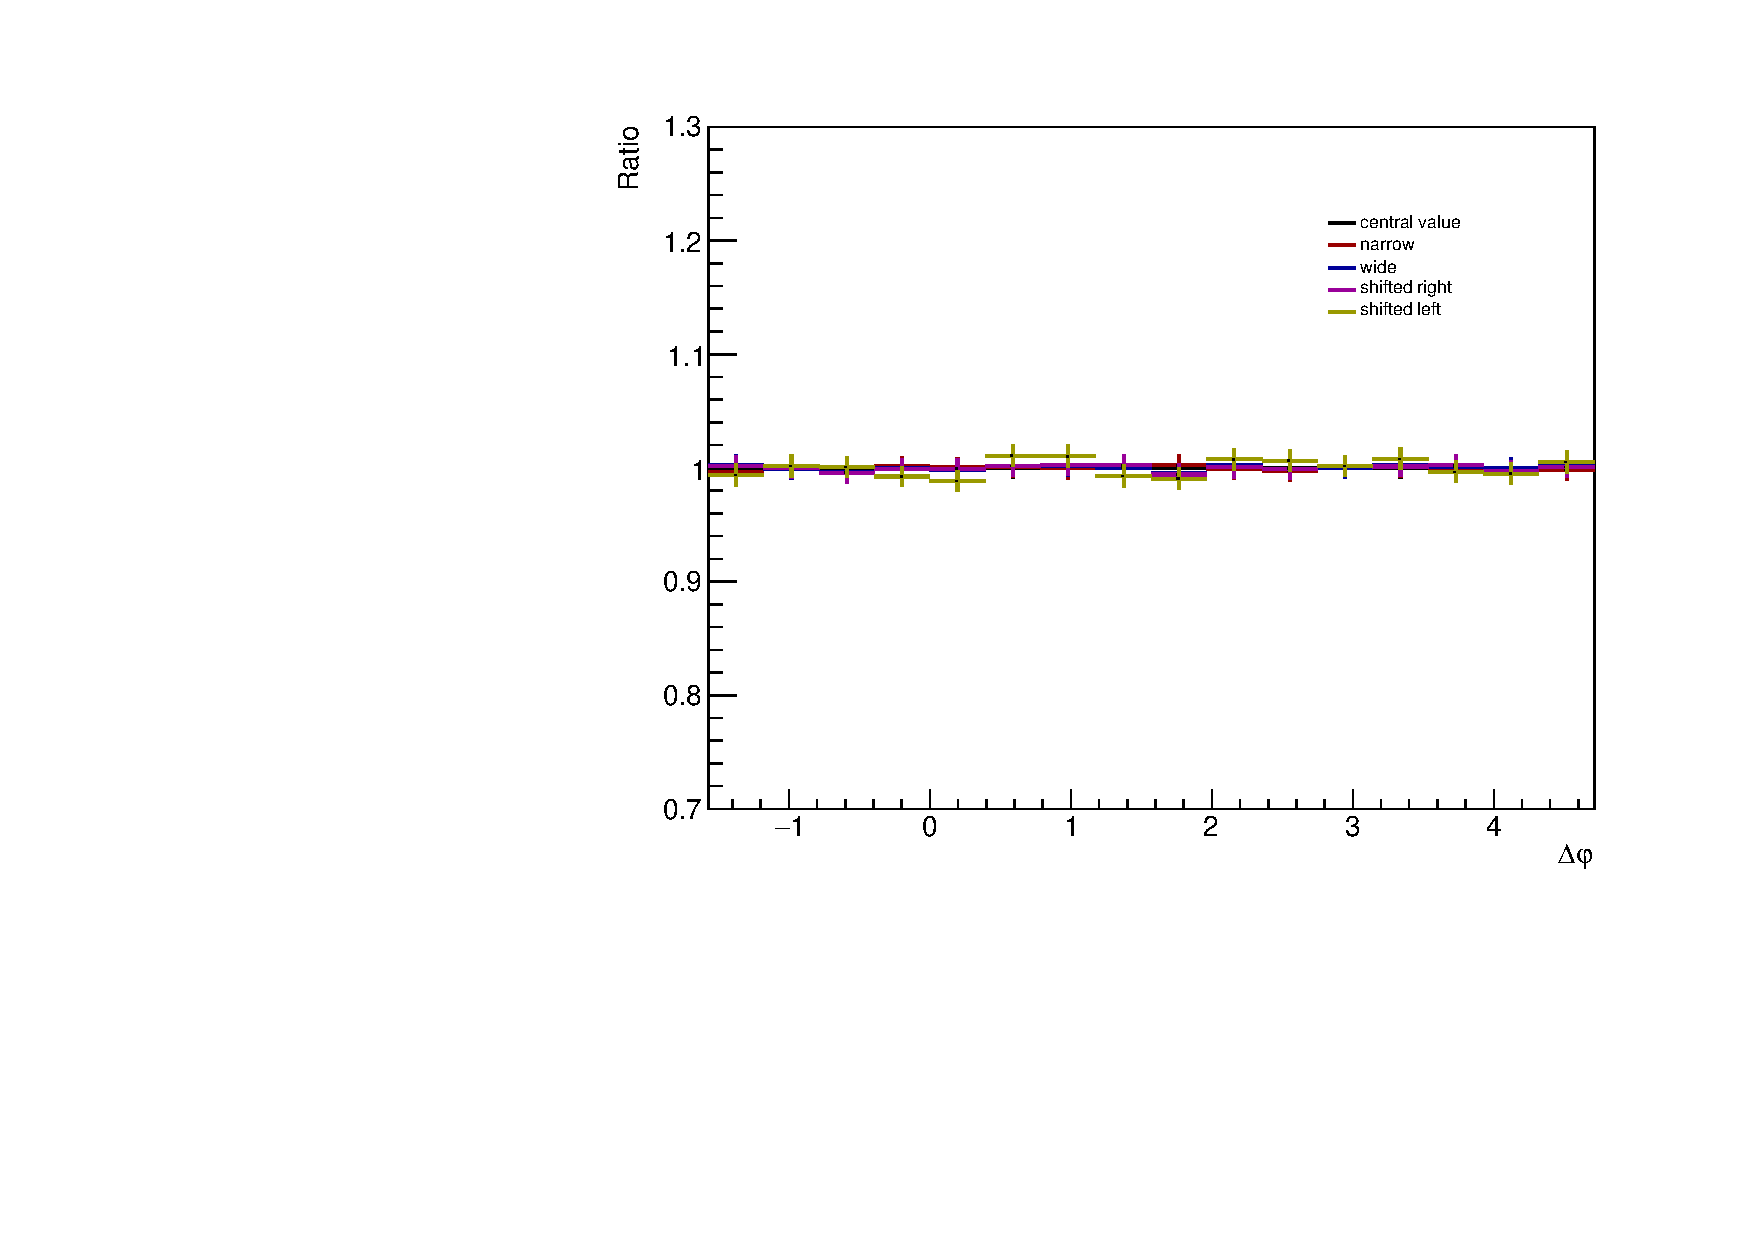
\includegraphics[width=0.49\textwidth]{figures/analysis/sideband_variations_dphi_0_20_lowpt_ratio.pdf}
    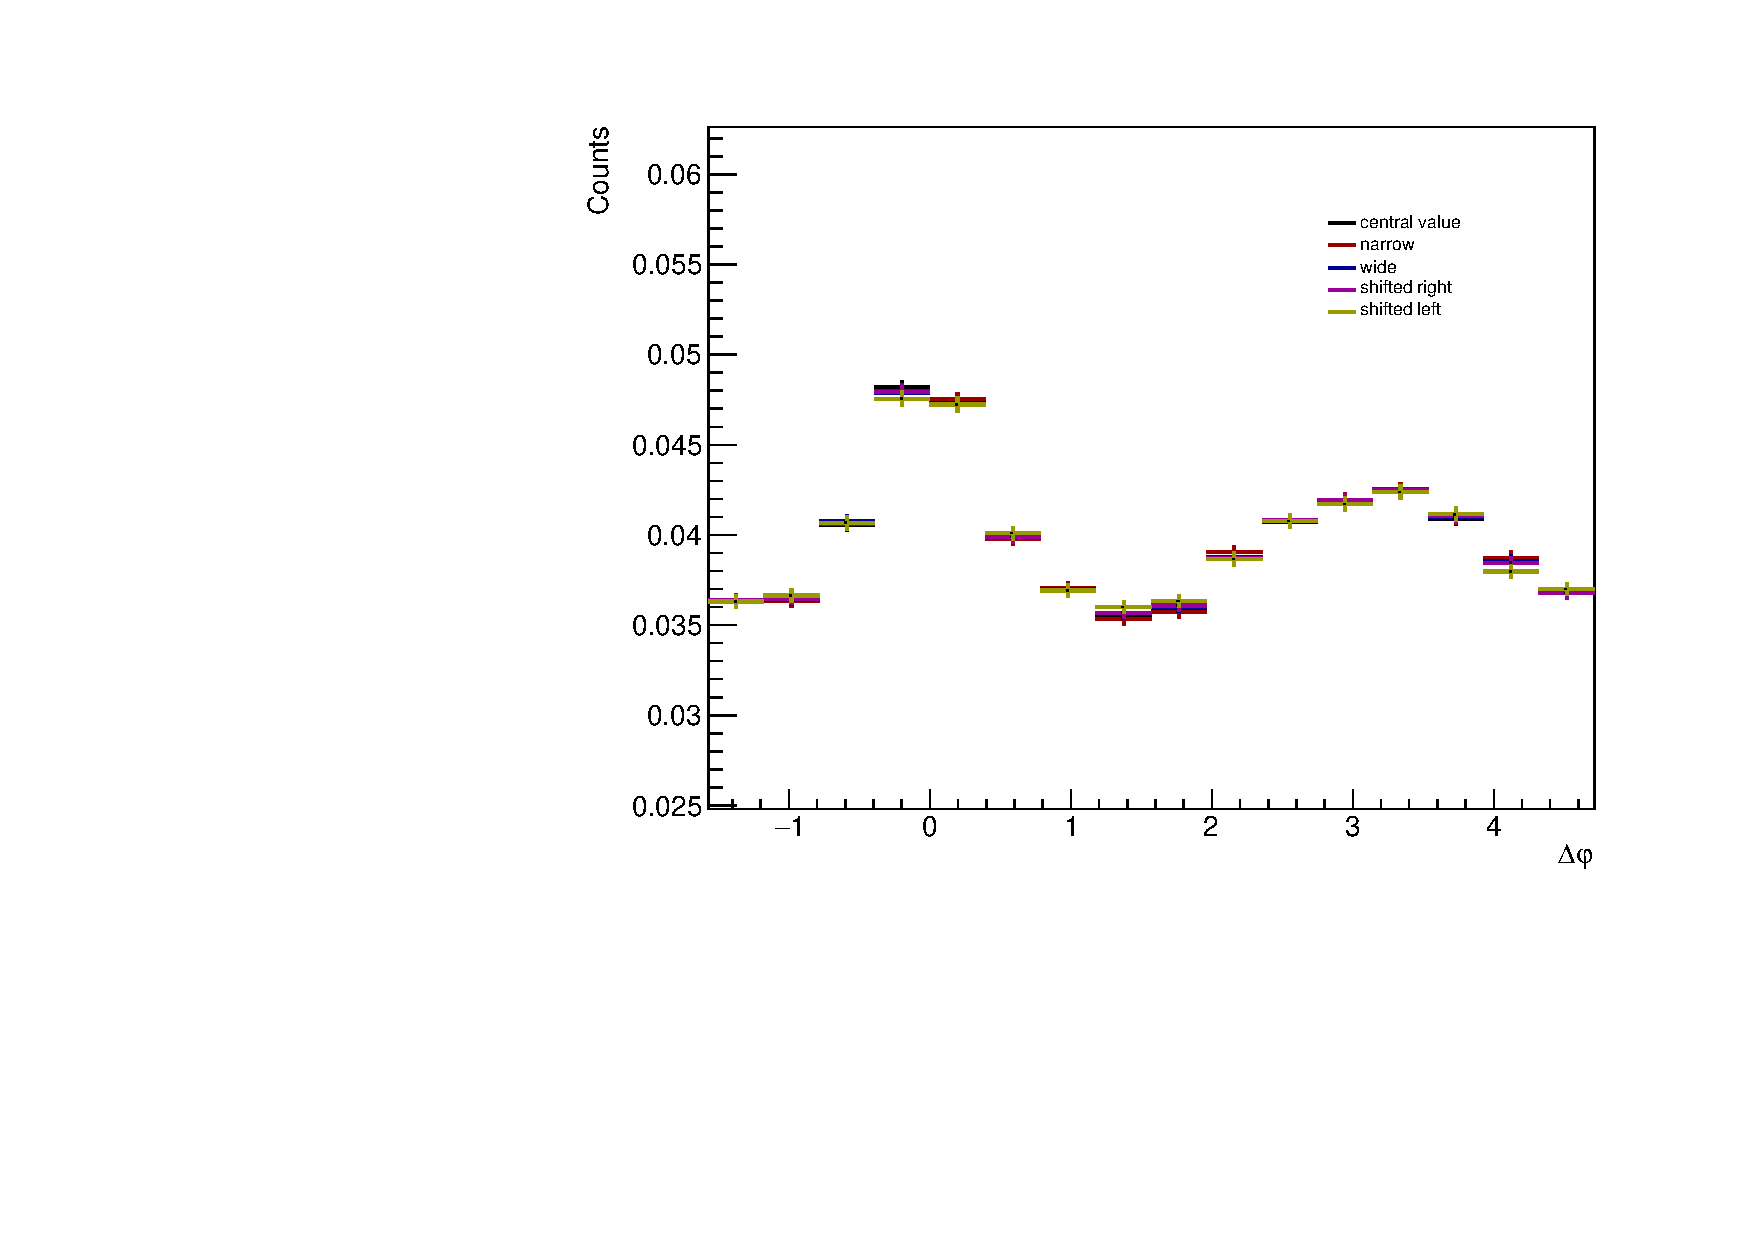
\includegraphics[width=0.49\textwidth]{figures/analysis/sideband_variations_dphi_20_50_lowpt.pdf}
    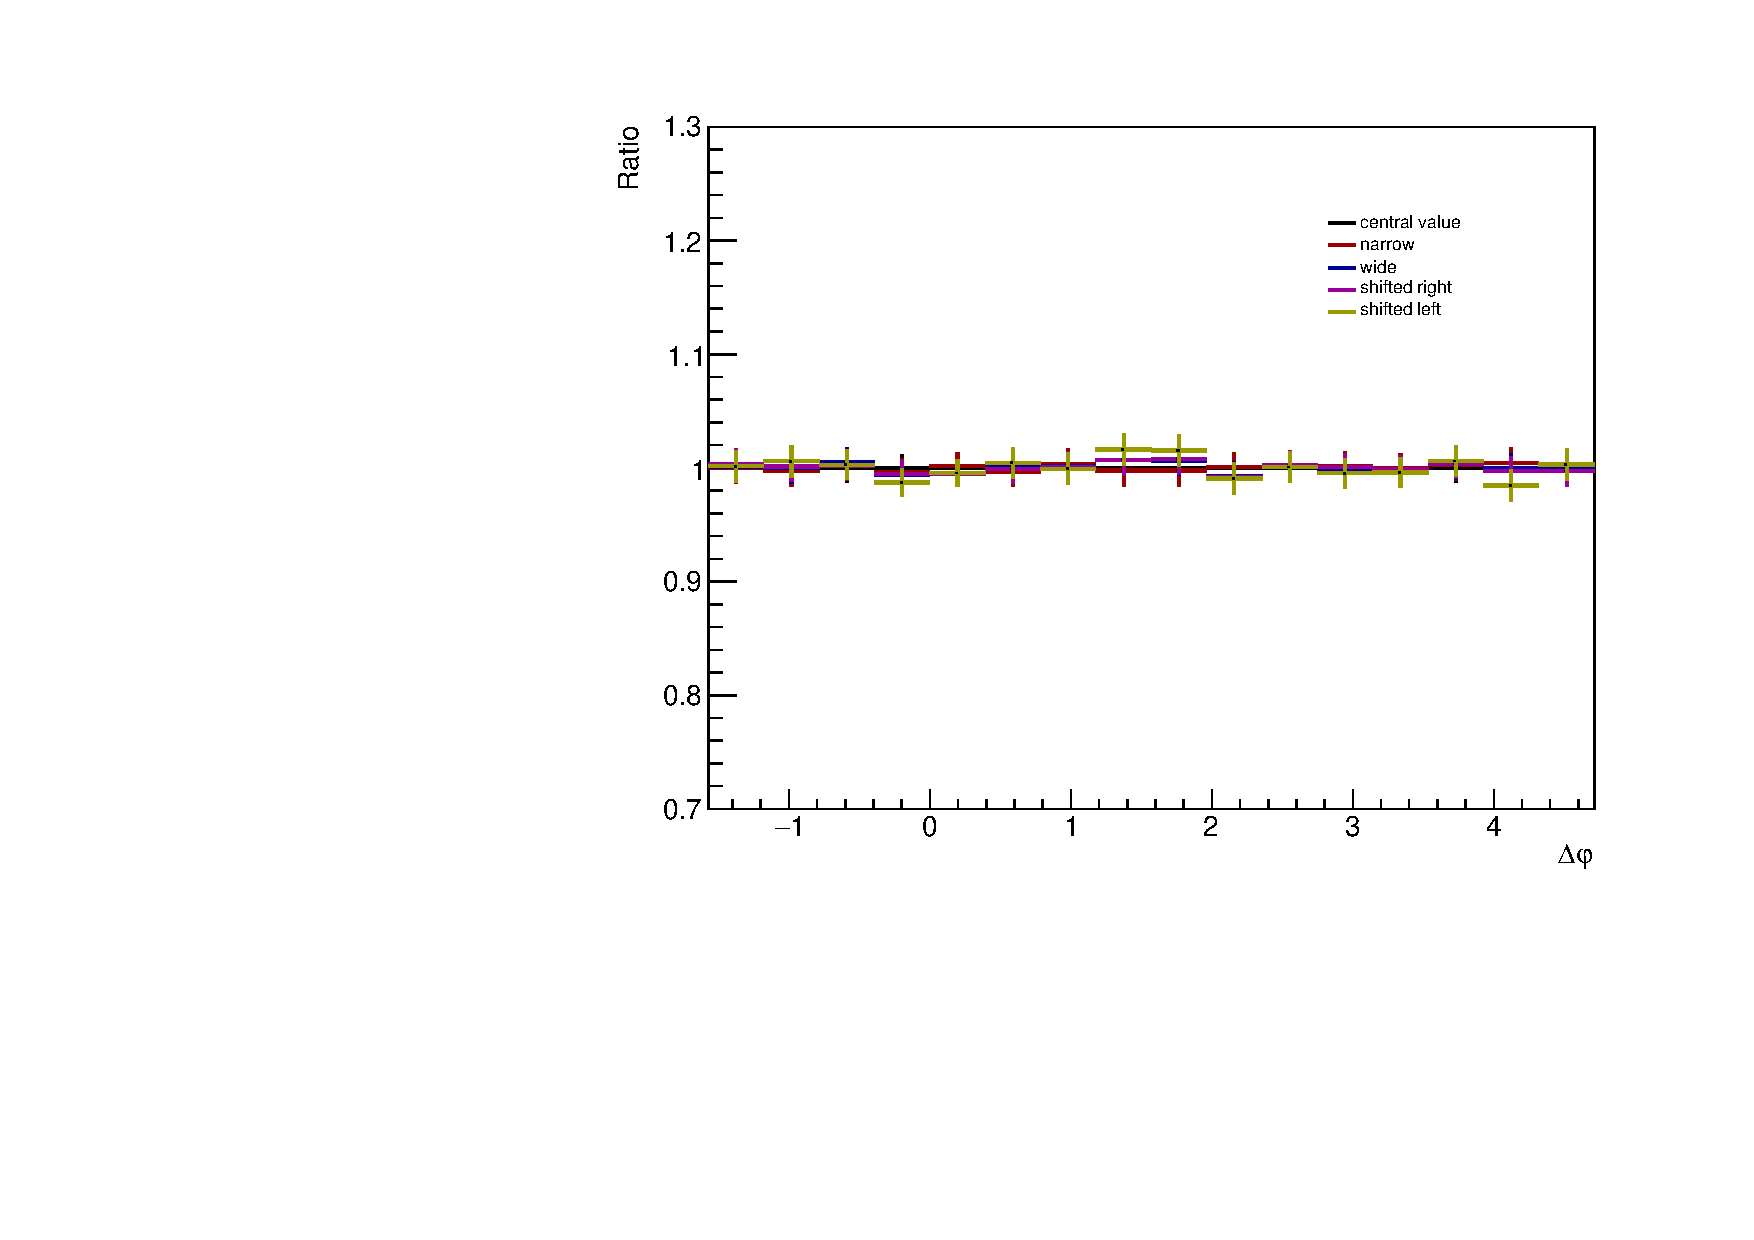
\includegraphics[width=0.49\textwidth]{figures/analysis/sideband_variations_dphi_20_50_lowpt_ratio.pdf}
    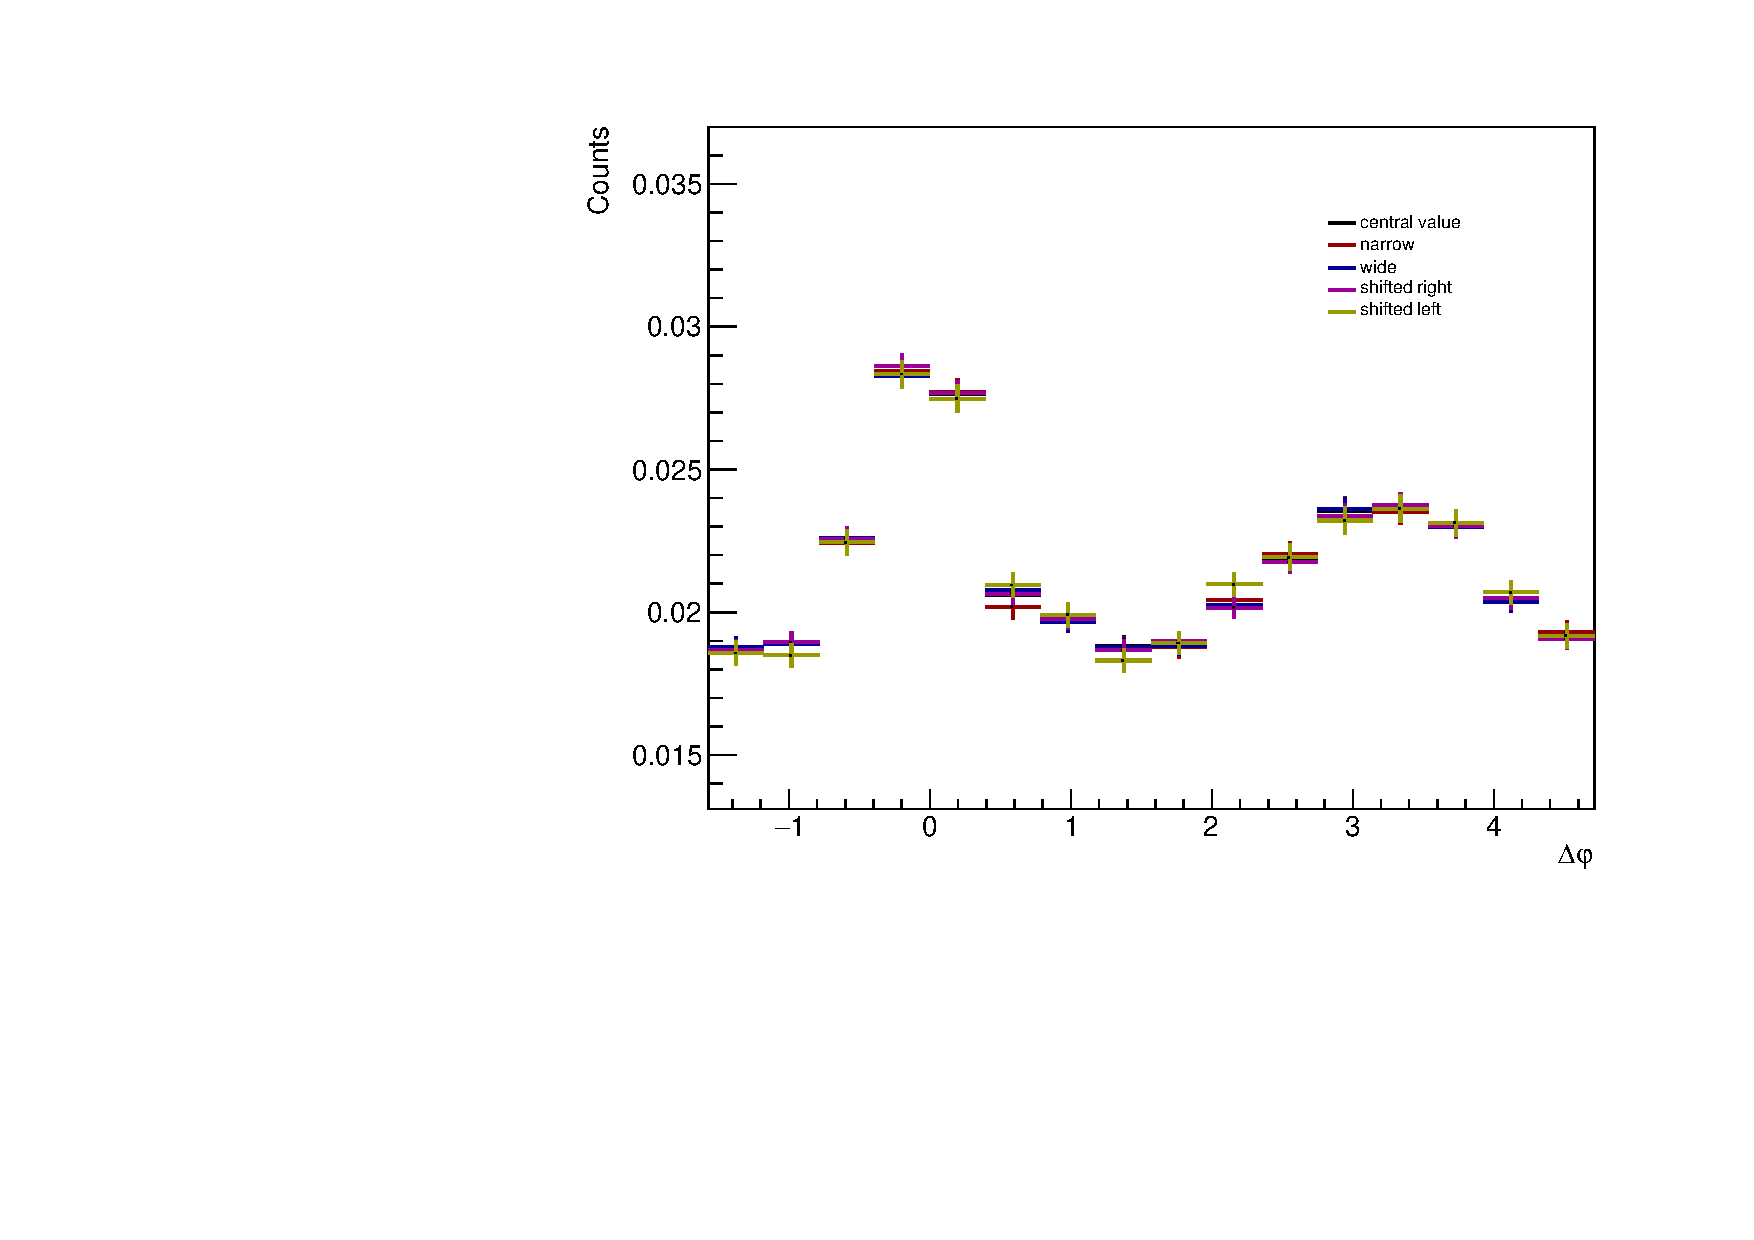
\includegraphics[width=0.49\textwidth]{figures/analysis/sideband_variations_dphi_50_80_lowpt.pdf}
    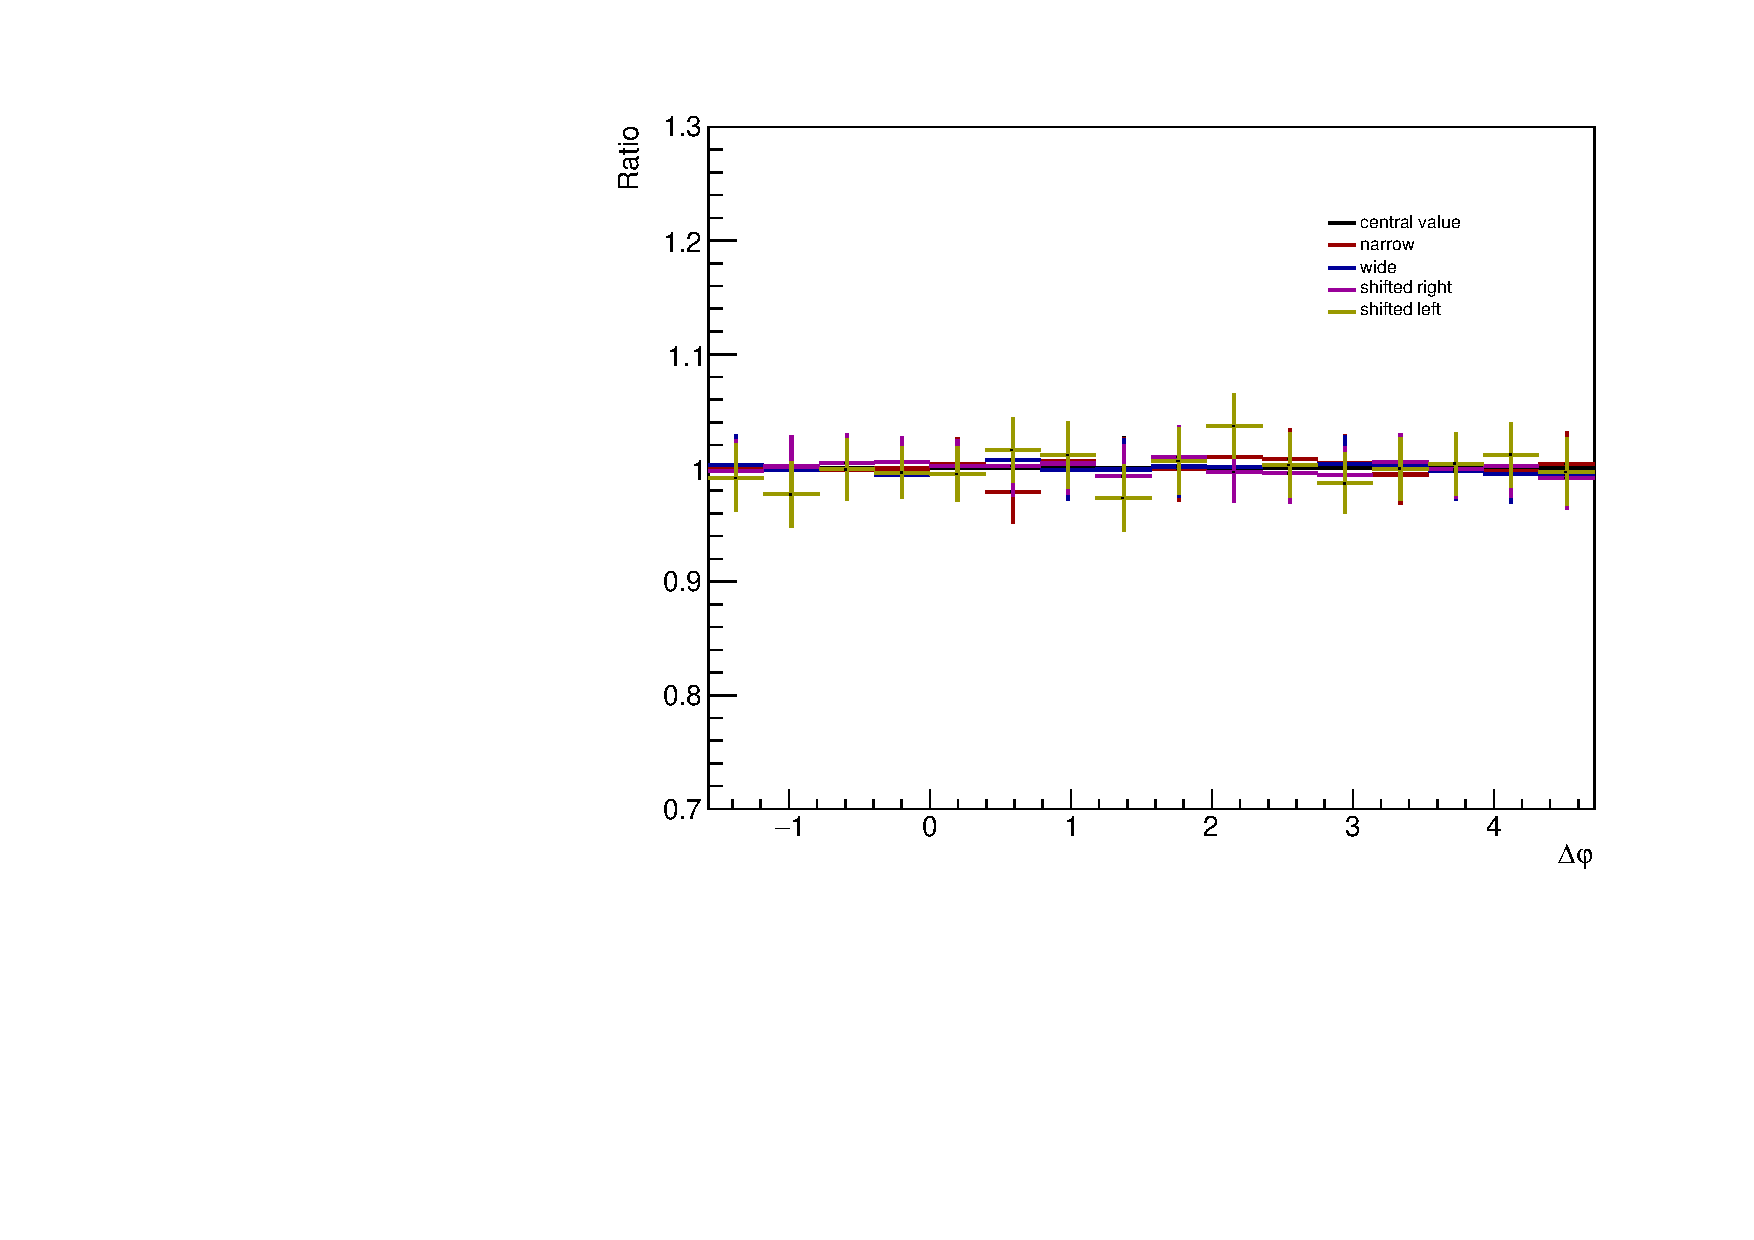
\includegraphics[width=0.49\textwidth]{figures/analysis/sideband_variations_dphi_50_80_lowpt_ratio.pdf}
    \caption{The h-\lmb $\Delta\varphi$ distributions within the 0-20\% (top), 20-50\% (middle) and 50-80\% (bottom) multiplicity bins in the lower associated \pt bin for each of the sideband region variations (left) with the ratios to the nominal distribution (right).}
    \label{fig:sideband_region_variations_lowpt}
\end{figure}

\begin{figure}[ht]
    \centering
    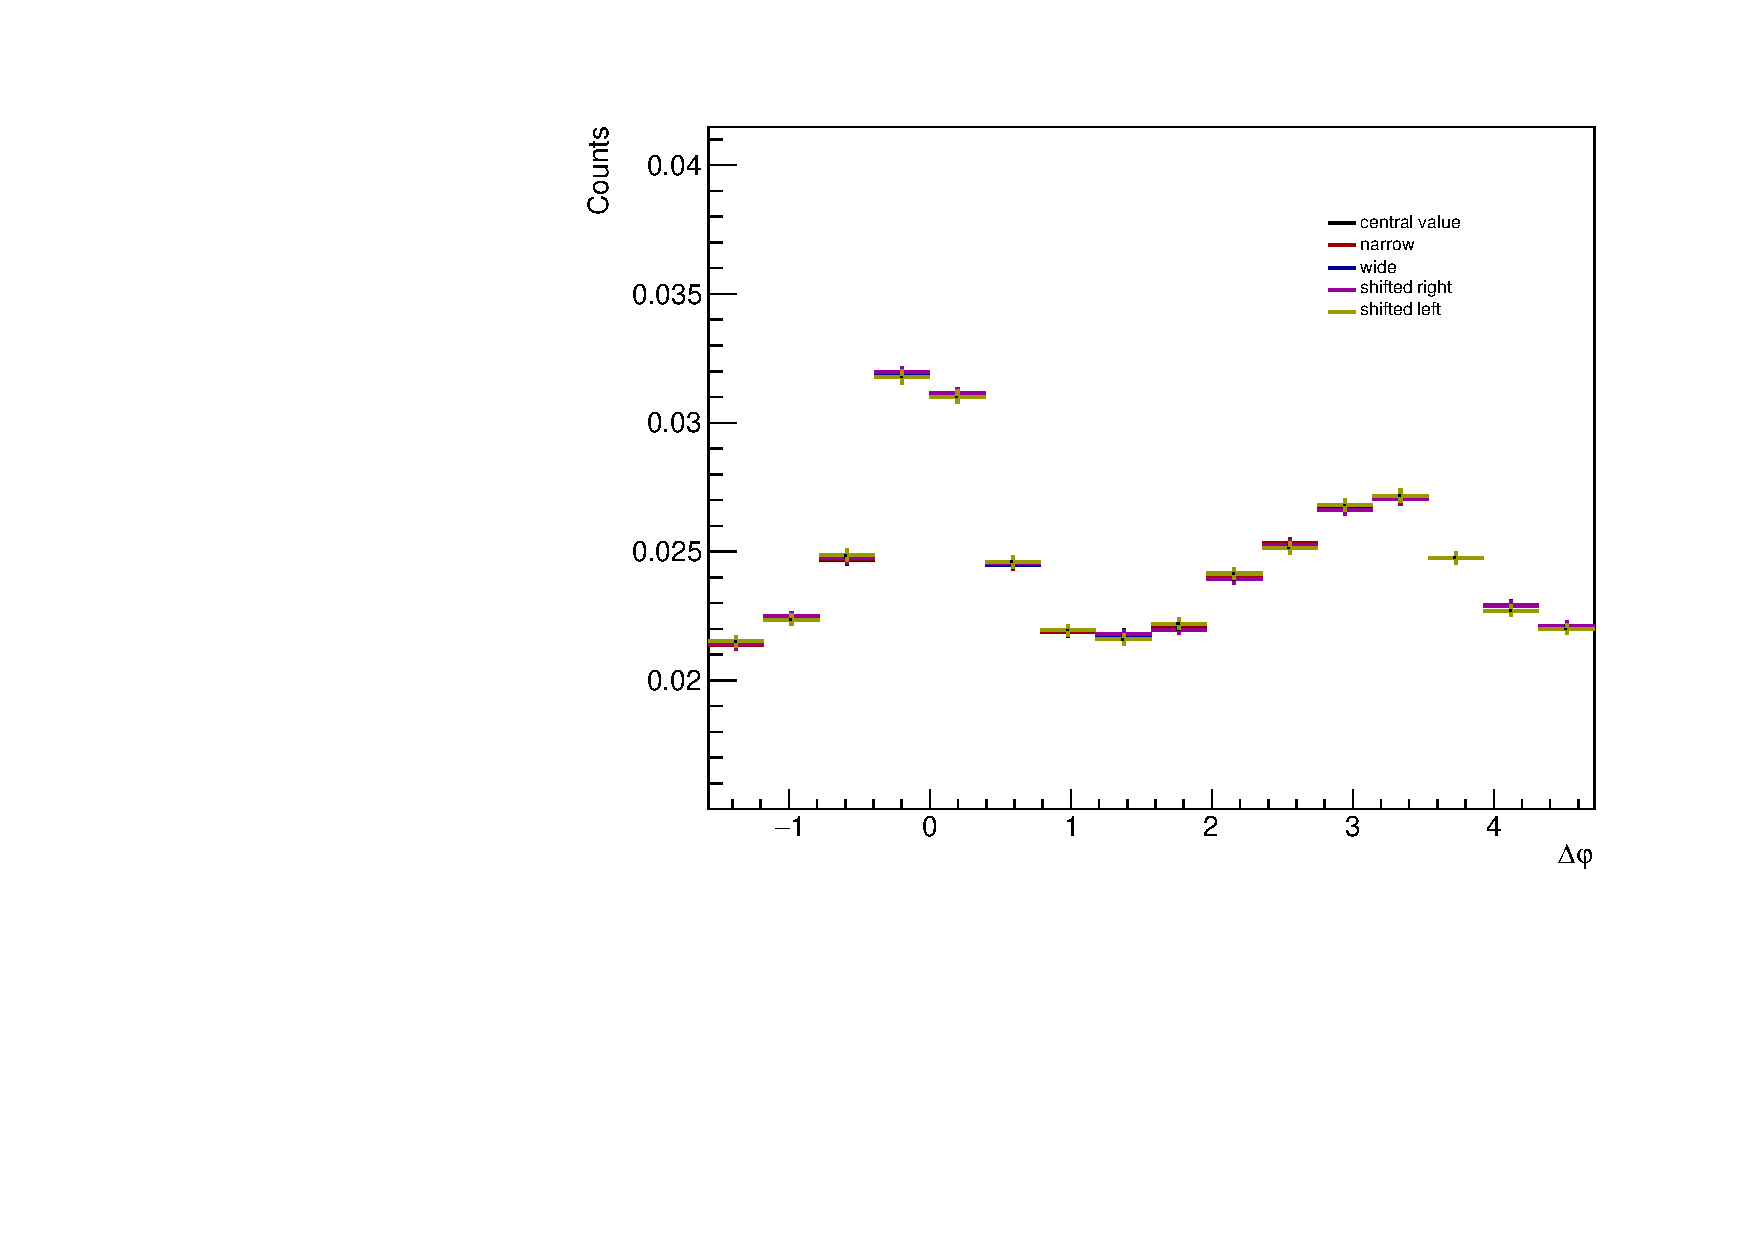
\includegraphics[width=0.49\textwidth]{figures/analysis/sideband_variations_dphi_0_20_highpt.pdf}
    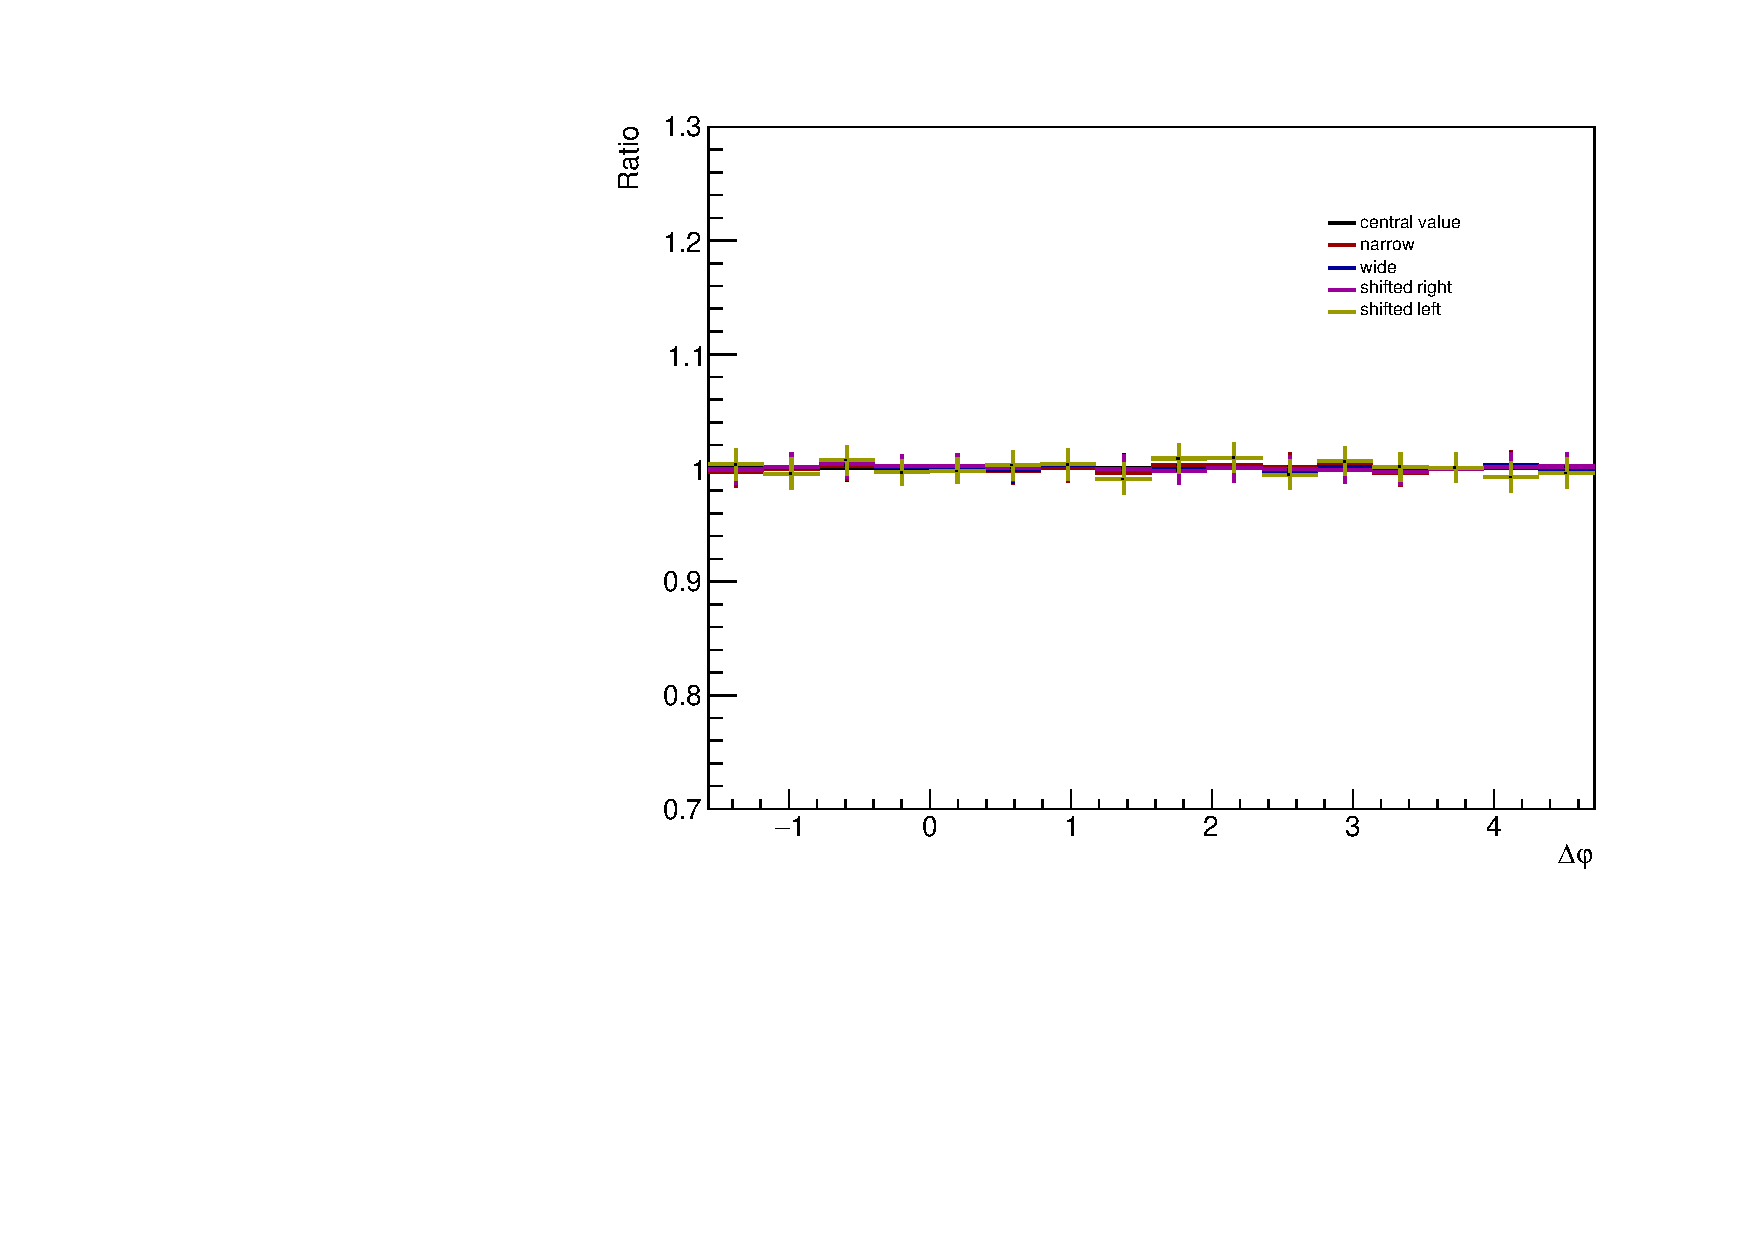
\includegraphics[width=0.49\textwidth]{figures/analysis/sideband_variations_dphi_0_20_highpt_ratio.pdf}
    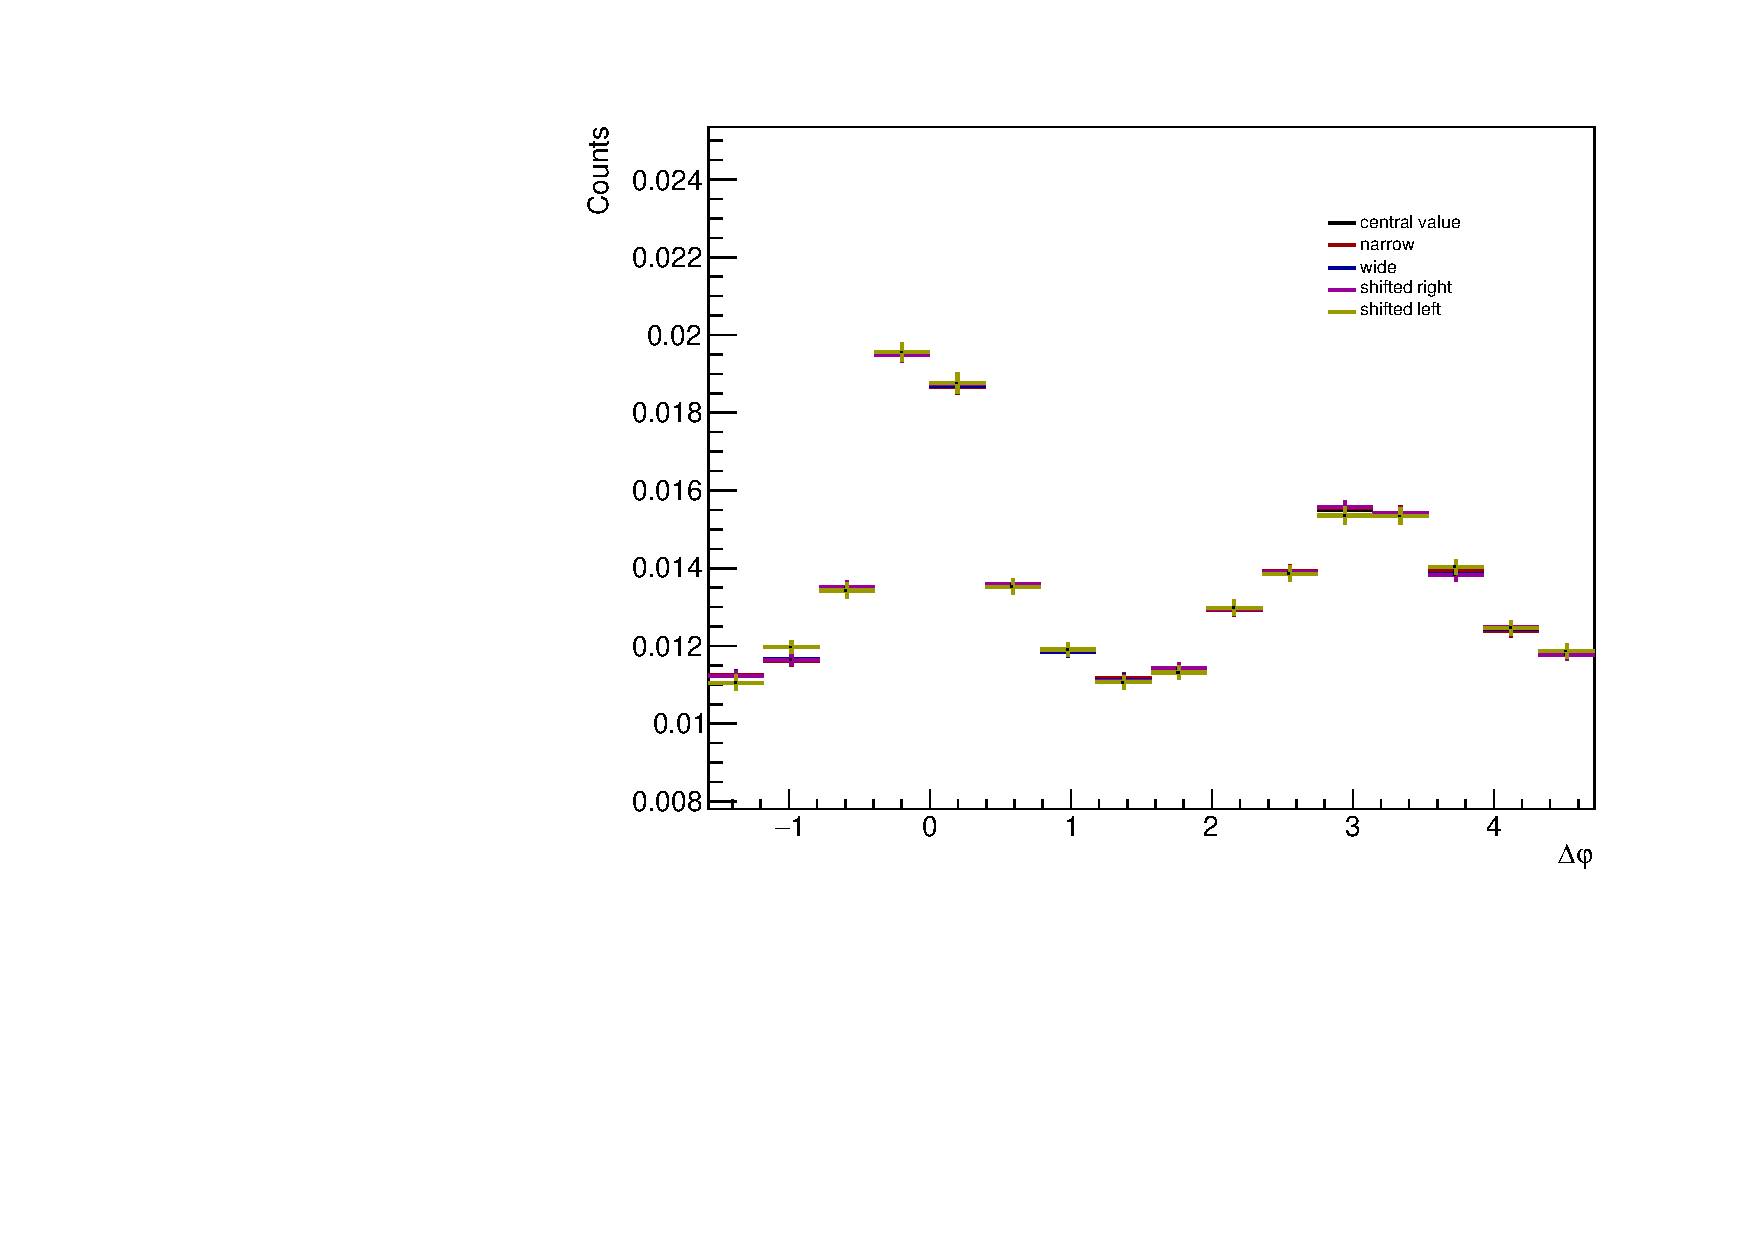
\includegraphics[width=0.49\textwidth]{figures/analysis/sideband_variations_dphi_20_50_highpt.pdf}
    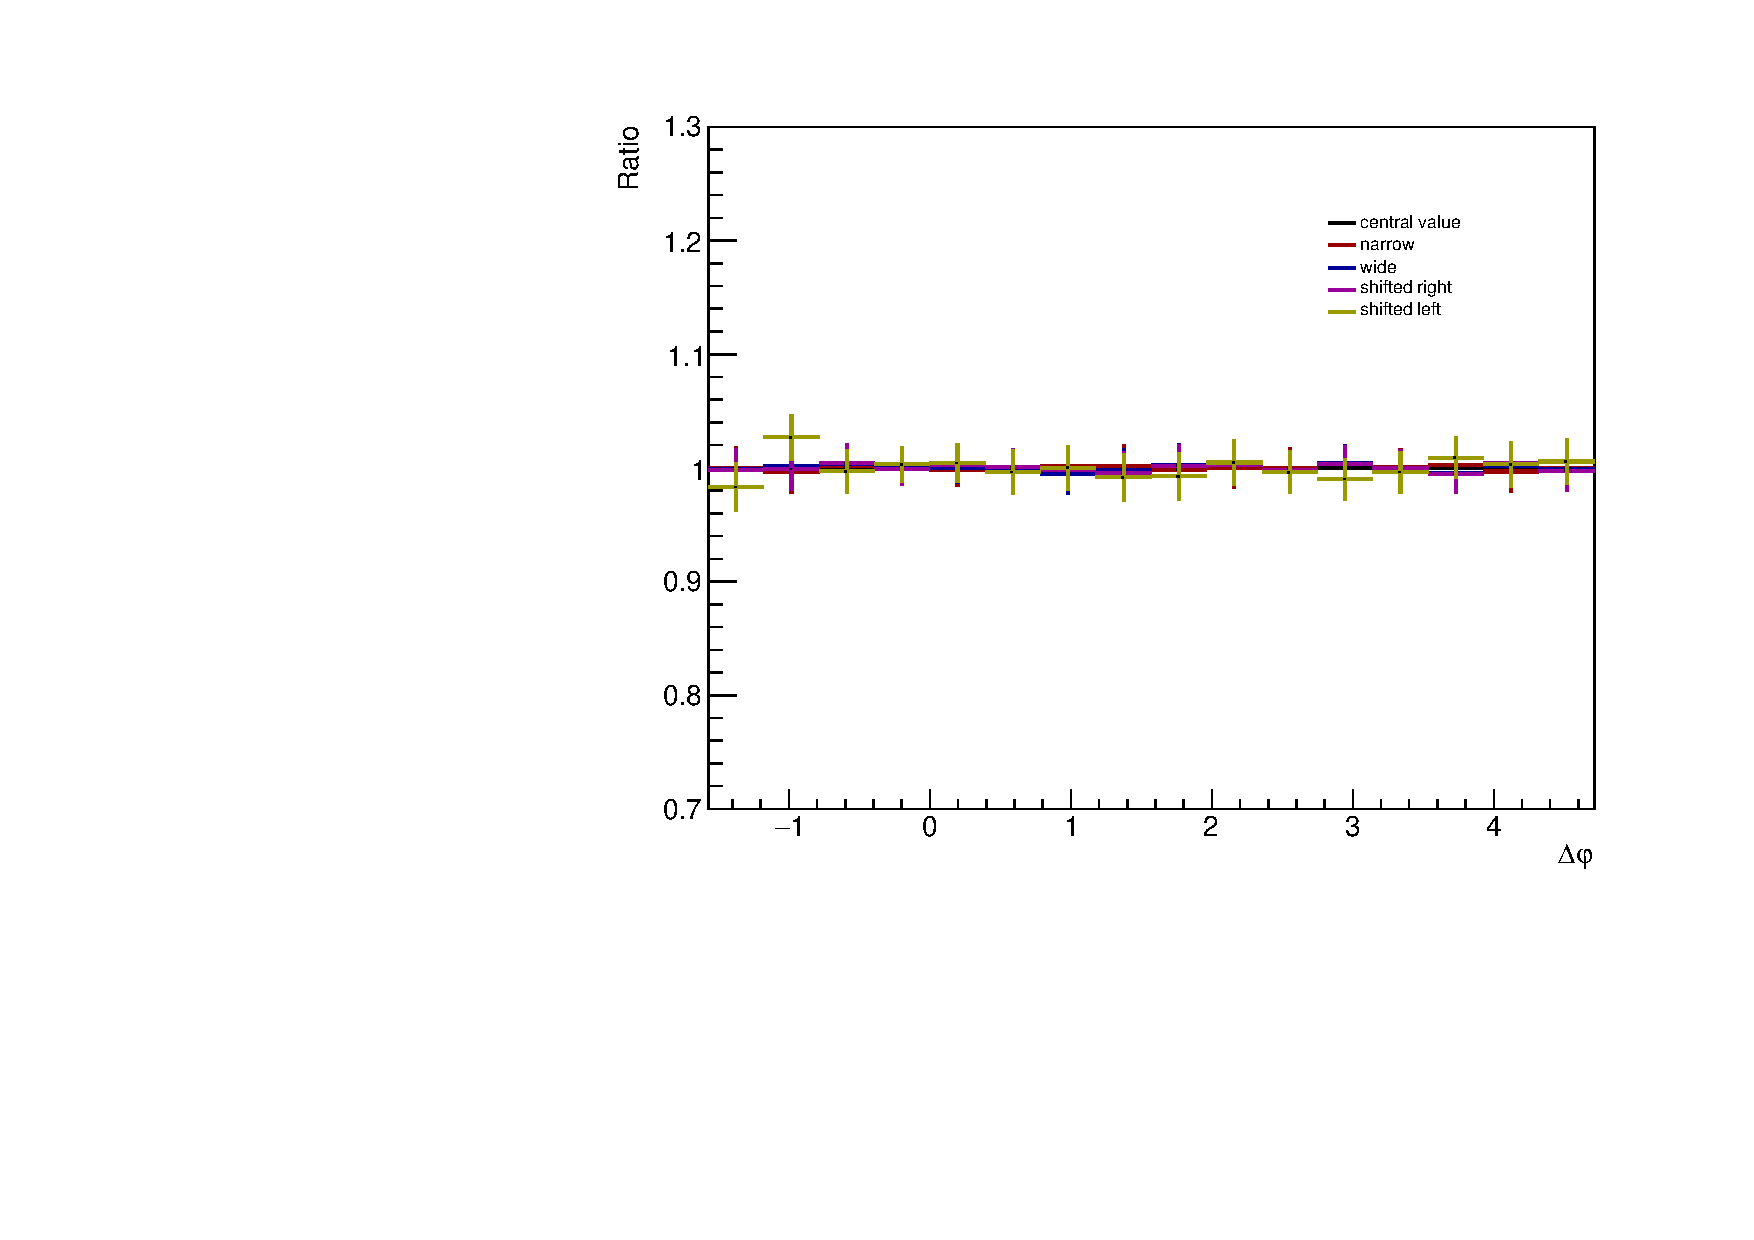
\includegraphics[width=0.49\textwidth]{figures/analysis/sideband_variations_dphi_20_50_highpt_ratio.pdf}
    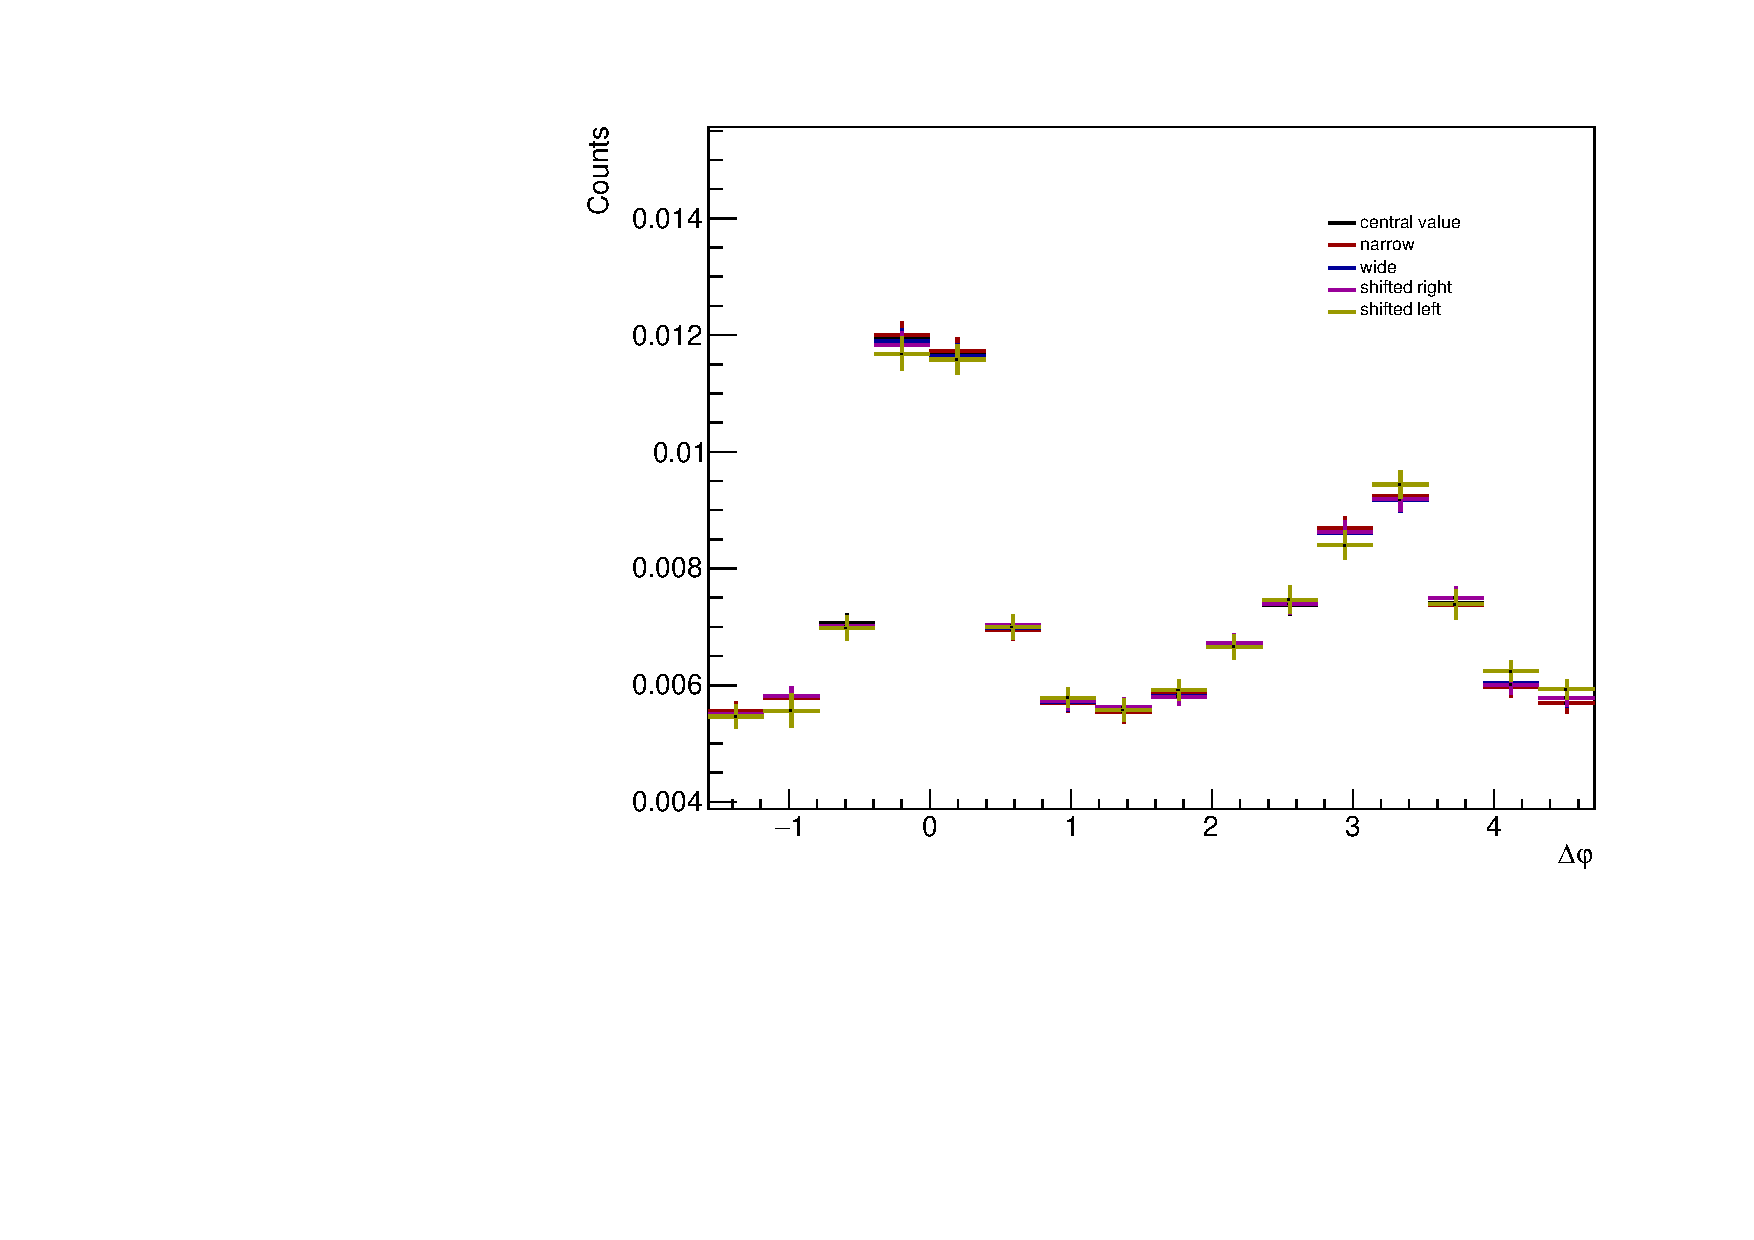
\includegraphics[width=0.49\textwidth]{figures/analysis/sideband_variations_dphi_50_80_highpt.pdf}
    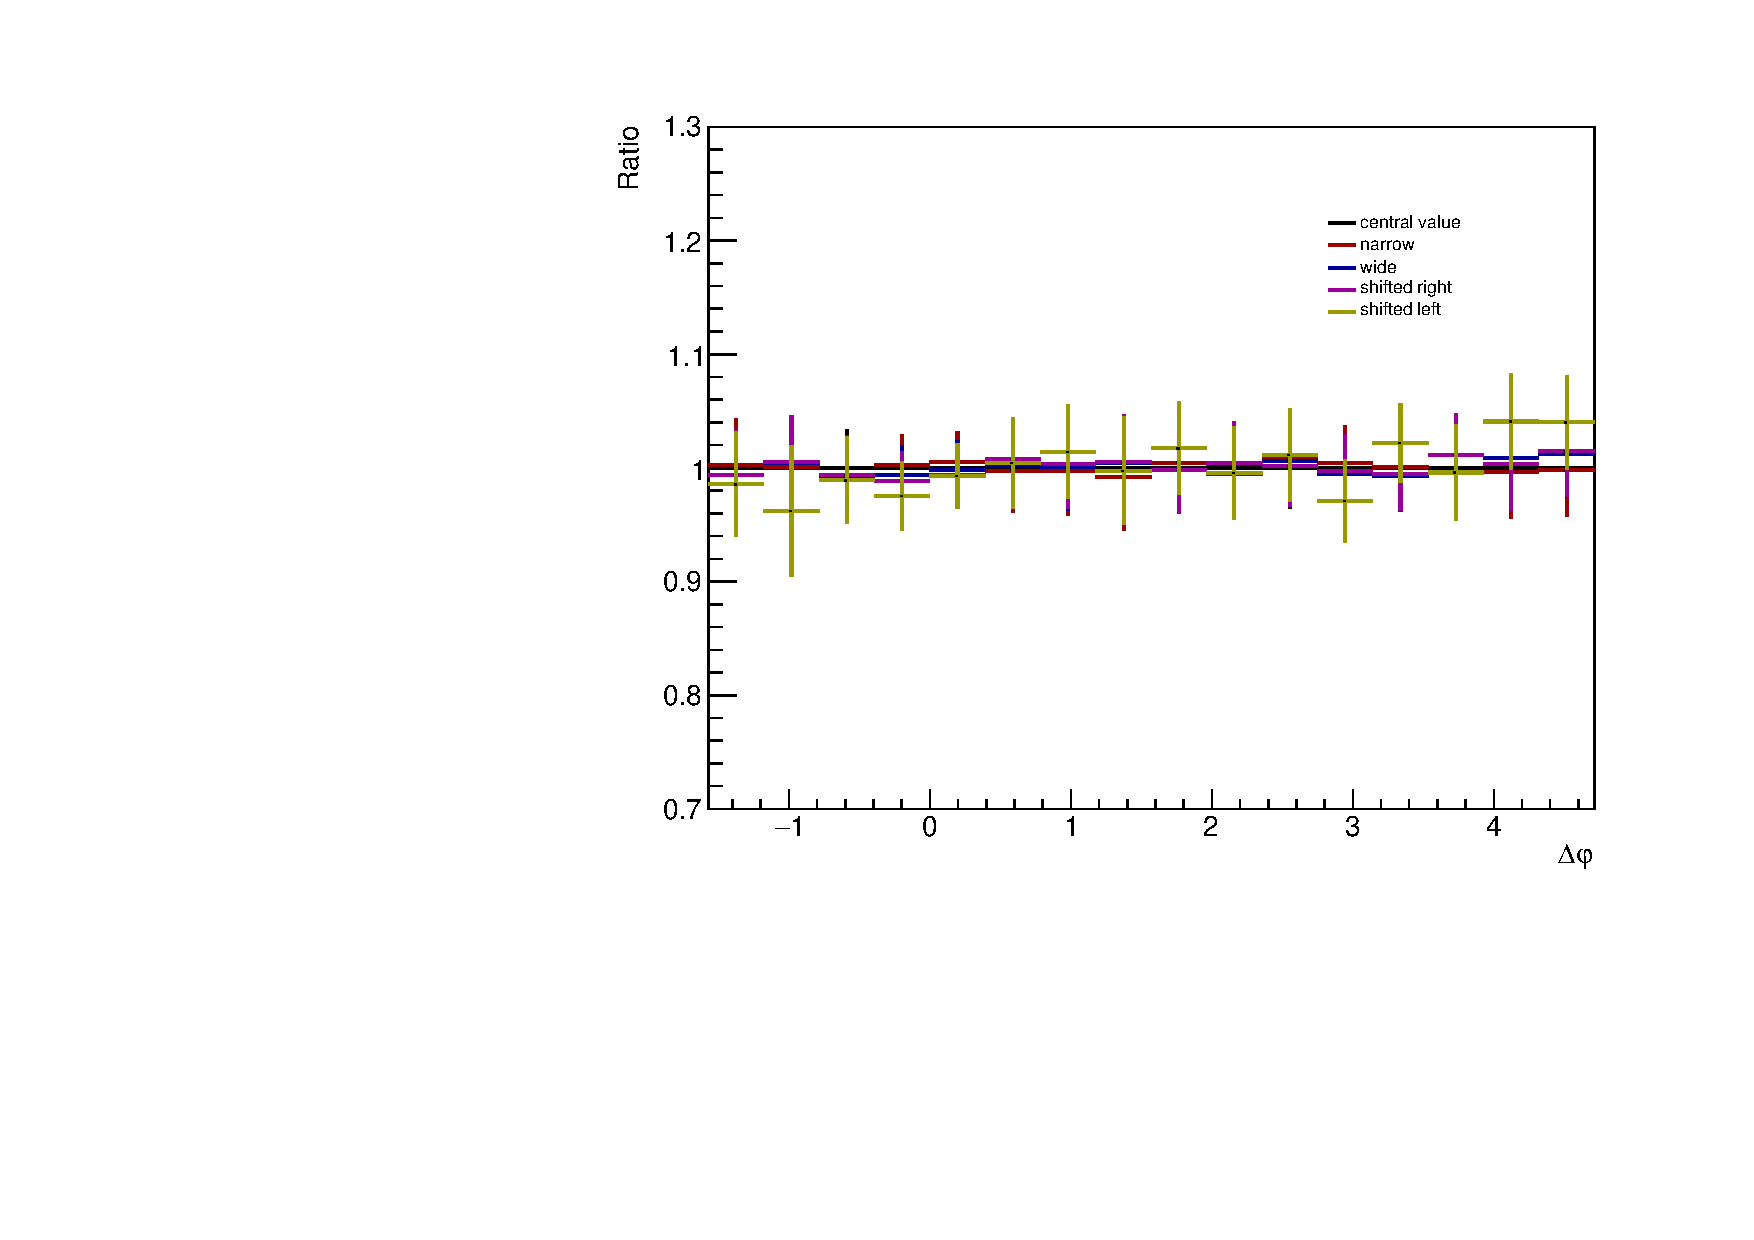
\includegraphics[width=0.49\textwidth]{figures/analysis/sideband_variations_dphi_50_80_highpt_ratio.pdf}
    \caption{The h-\lmb $\Delta\varphi$ distributions within the 0-20\% (top), 20-50\% (middle) and 50-80\% (bottom) multiplicity bins in the higher associated \pt bin for each of the sideband region variations (left) with the ratios to the nominal distribution (right).}
    \label{fig:sideband_region_variations_highpt}
\end{figure}

\subsubsection{\lmb daughter particle identification}
The \lmb daughter particle identification (PID) cuts are chosen to be wide enough to ensure a high efficiency, but narrow enough to ensure a high purity. As the requirement for a higher purity should be offset by the subtraction of the combinatorial background, altering the PID cuts should only minimally effect the final $\Delta\varphi$ distributions. To study this, the PID cuts are varied in the ways presented in Table~\ref{tab:pid_cut_variations}. The final $\Delta\varphi$ distributions and ratios to the nominal distribution for each PID cut variation in each multiplicity and associated \pt bin are shown in Figures \ref{fig:pid_cut_variations_lowpt} (lower \pt) and \ref{fig:pid_cut_variations_highpt} (higher \pt). Requiring a signal in the TOF detector drastically reduces the $\Lambda$ signal as the daugher pions are often heavily deflected by the magnetic field due to their lower \pt (again, $m_{\text{p}}/m_{\pi} \approx 7$, so most of the mother momentum belongs to the proton). This causes a large amount of statistical fluctuations in the corresponding $\Delta\varphi$ distribution, which is why the ``require TOF'' variation is inevitably excluded after the Barlow check presented in Section~\ref{sec:barlow_check_dphi}. The other variations result in only around a 2\% deviation from the nominal $\Delta\varphi$ distribution, on average.

\begin{table}[ht]
    \centering
    \caption{The variations of the \lmb daughter PID cuts considered for this analysis. The ``require TOF'' variation requires a TOF hit for both the proton and pion, but maintains the nominal values for $|n\sigma_{\text{TPC, TOF}}|$.}
    \label{tab:pid_cut_variations}
    \begin{tabular}{l c c}
        \hline
        Variation name & $|n\sigma_{\text{TPC}, \text{TOF}}^{\pi}|$ & $|n\sigma_{\text{TPC}, \text{TOF}}^{\text{p}}|$ \\
        \hline
        Narrow & $< 1.8$ & $< 1.2$ \\
        Wide & $< 4.2$ & $< 2.8$ \\
        Require TOF & $< 3.0$ & $< 2.0$ \\
        \hline
    \end{tabular}
\end{table}

\begin{figure}[ht]
    \centering
    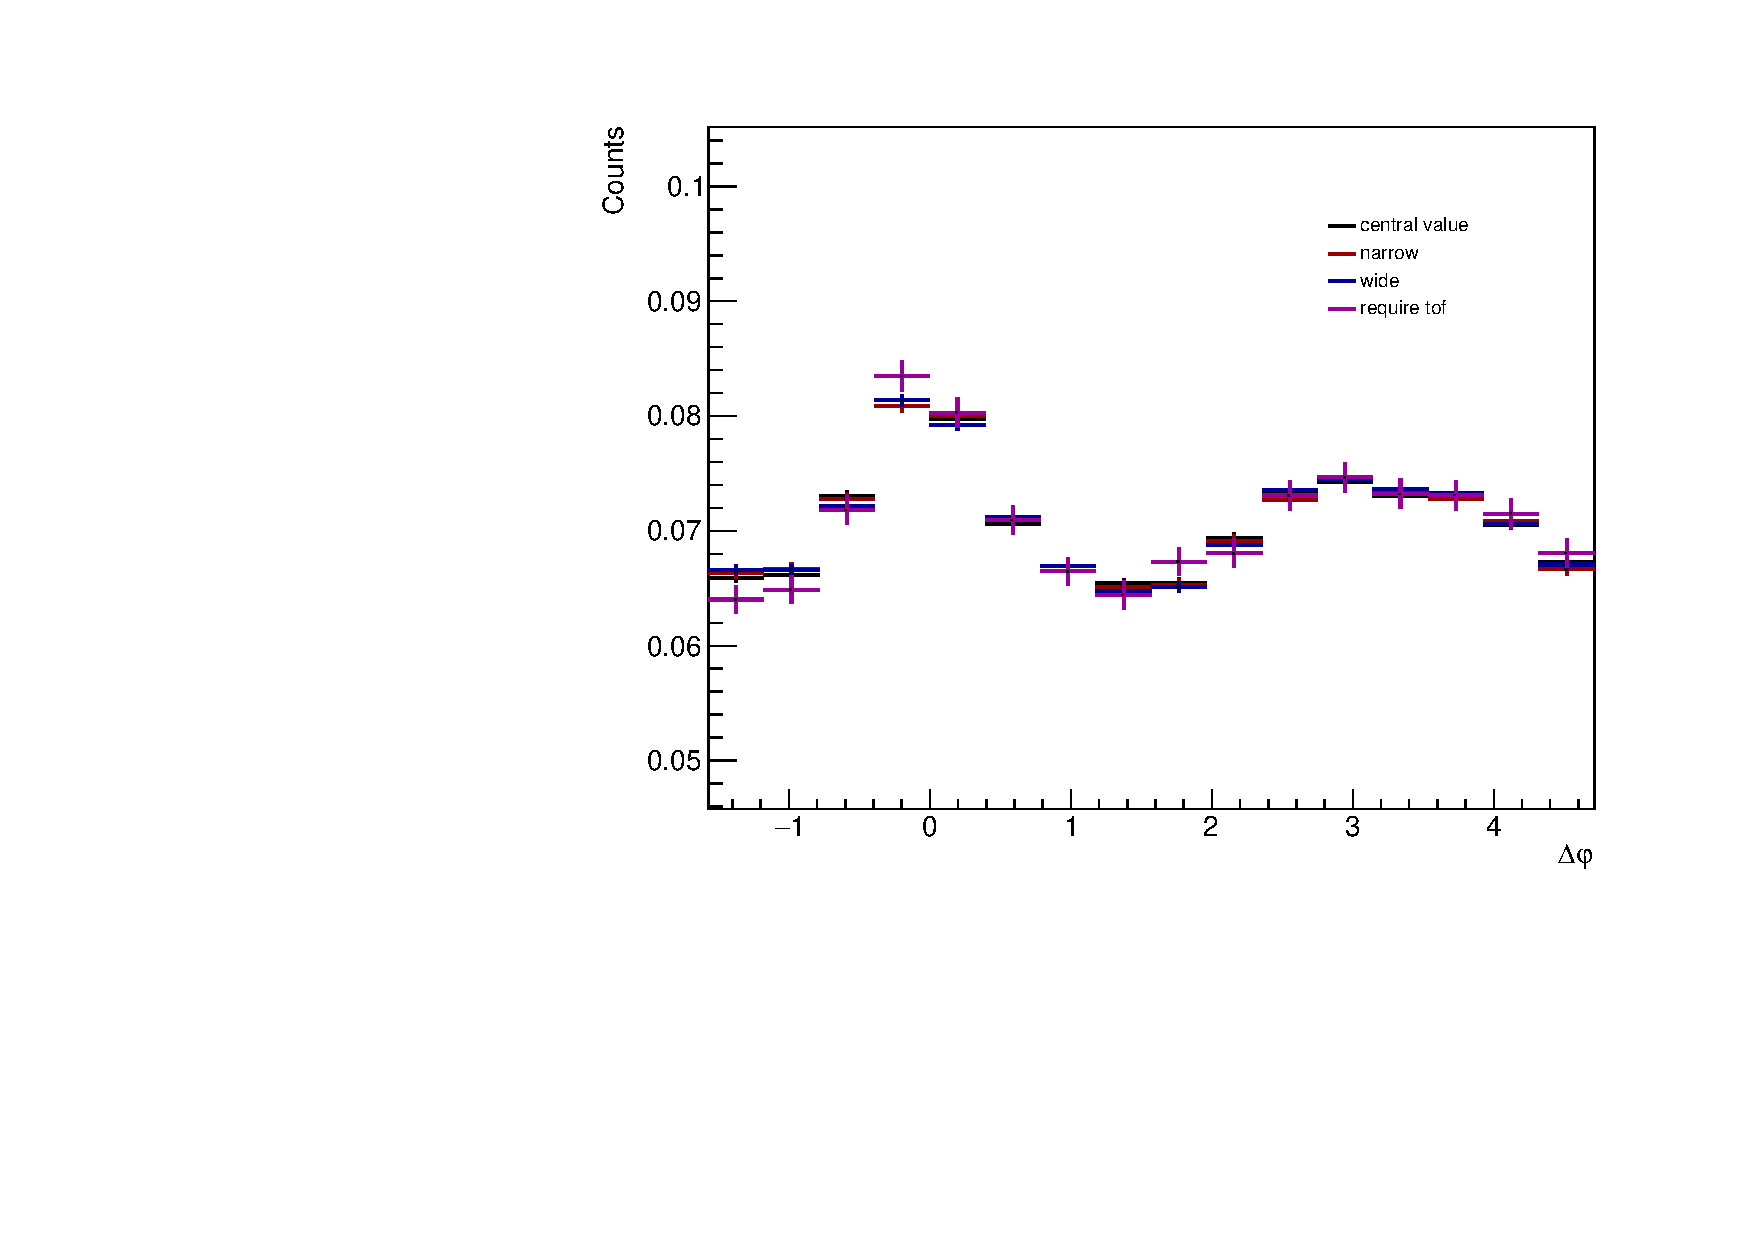
\includegraphics[width=0.49\textwidth]{figures/analysis/pid_variations_dphi_0_20_lowpt.pdf}
    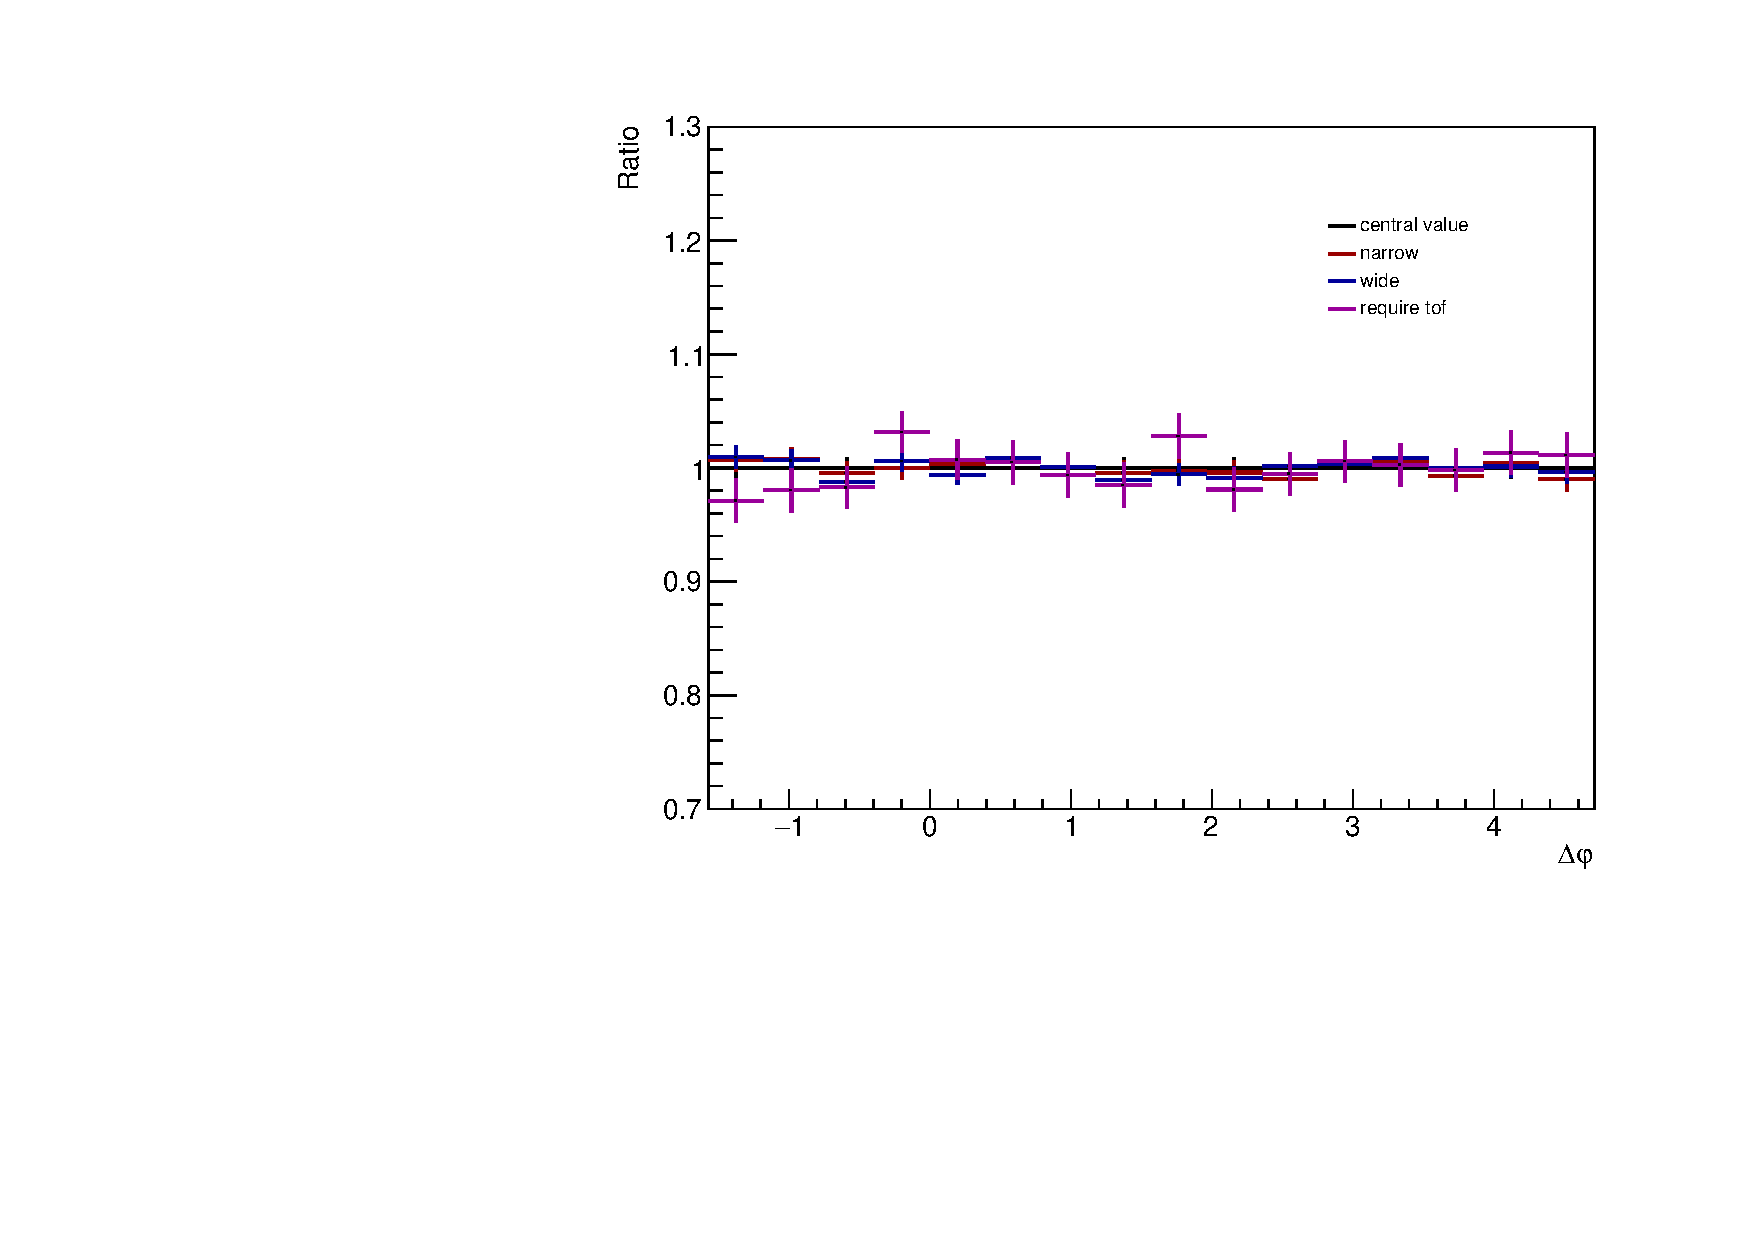
\includegraphics[width=0.49\textwidth]{figures/analysis/pid_variations_dphi_0_20_lowpt_ratio.pdf}
    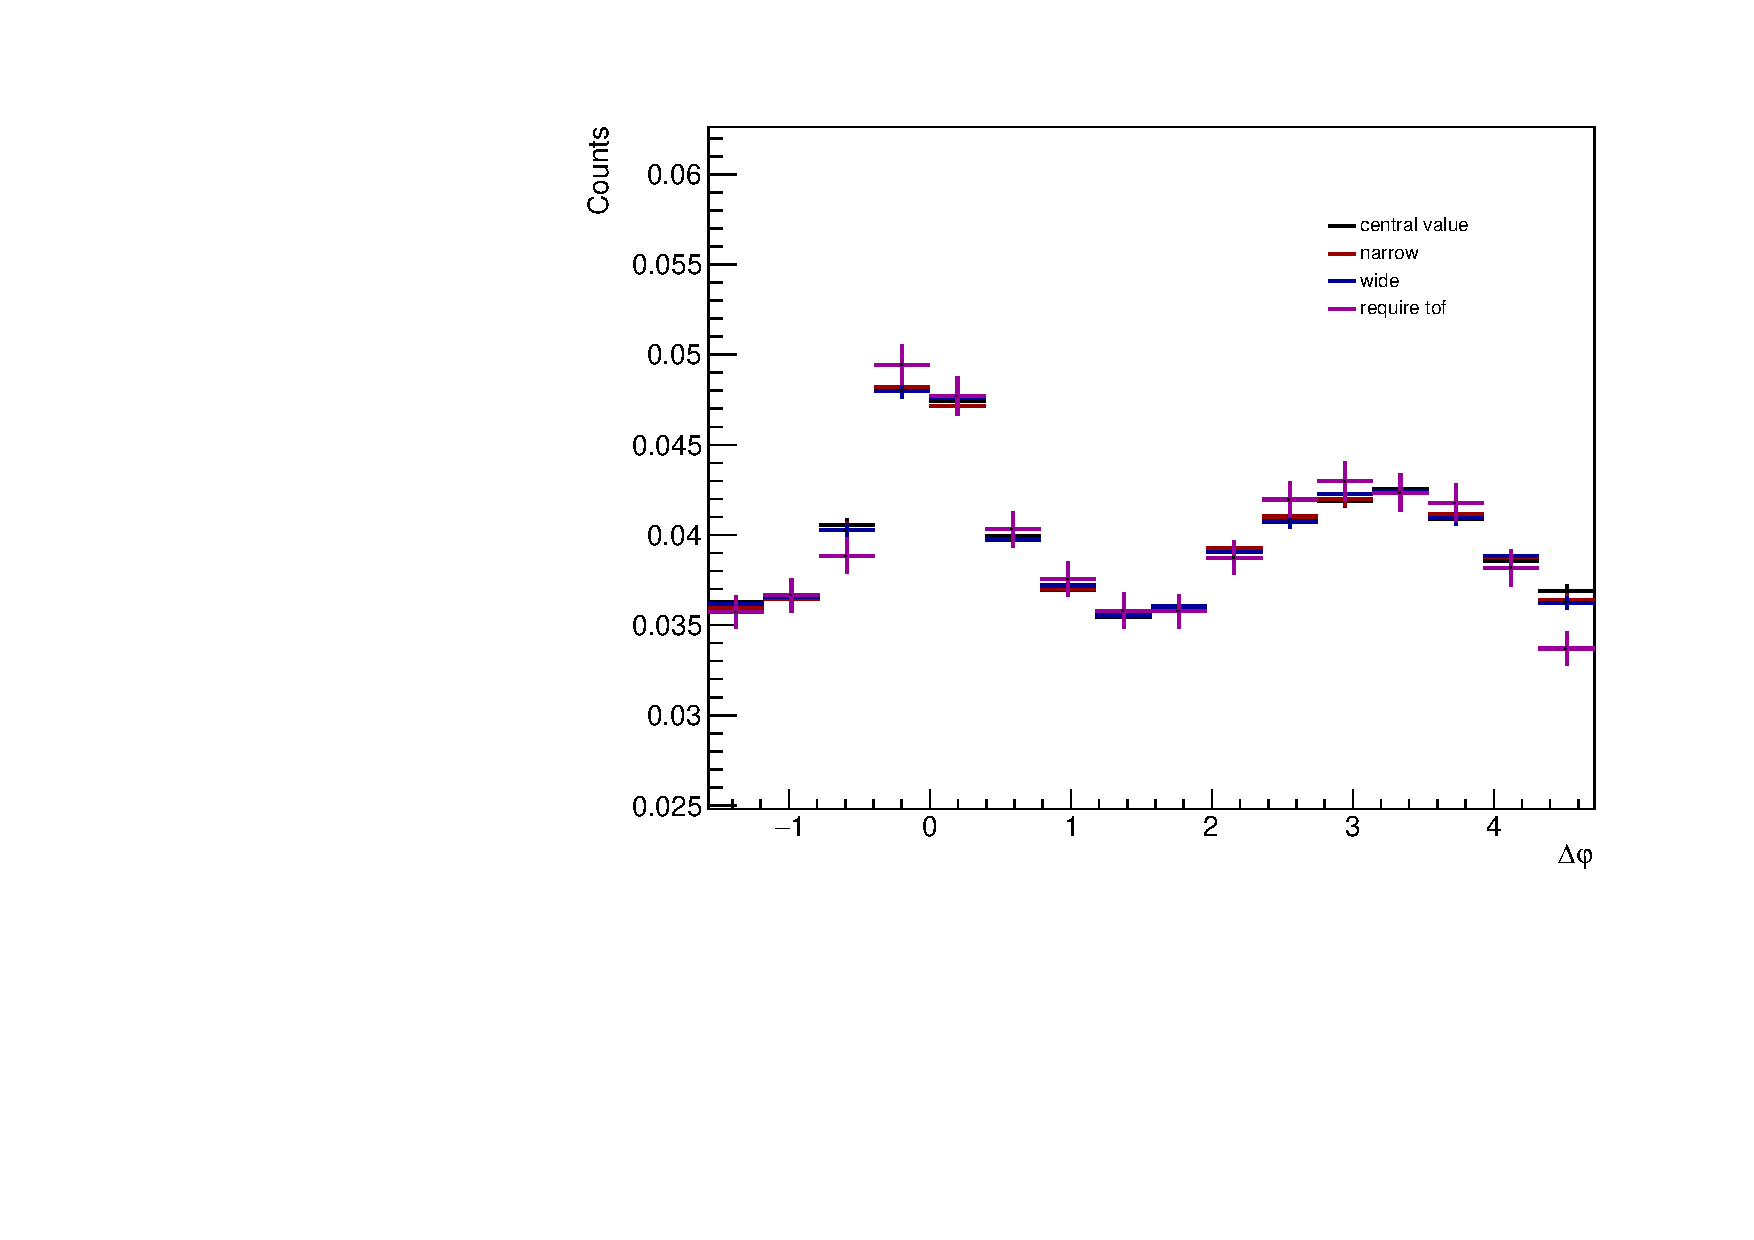
\includegraphics[width=0.49\textwidth]{figures/analysis/pid_variations_dphi_20_50_lowpt.pdf}
    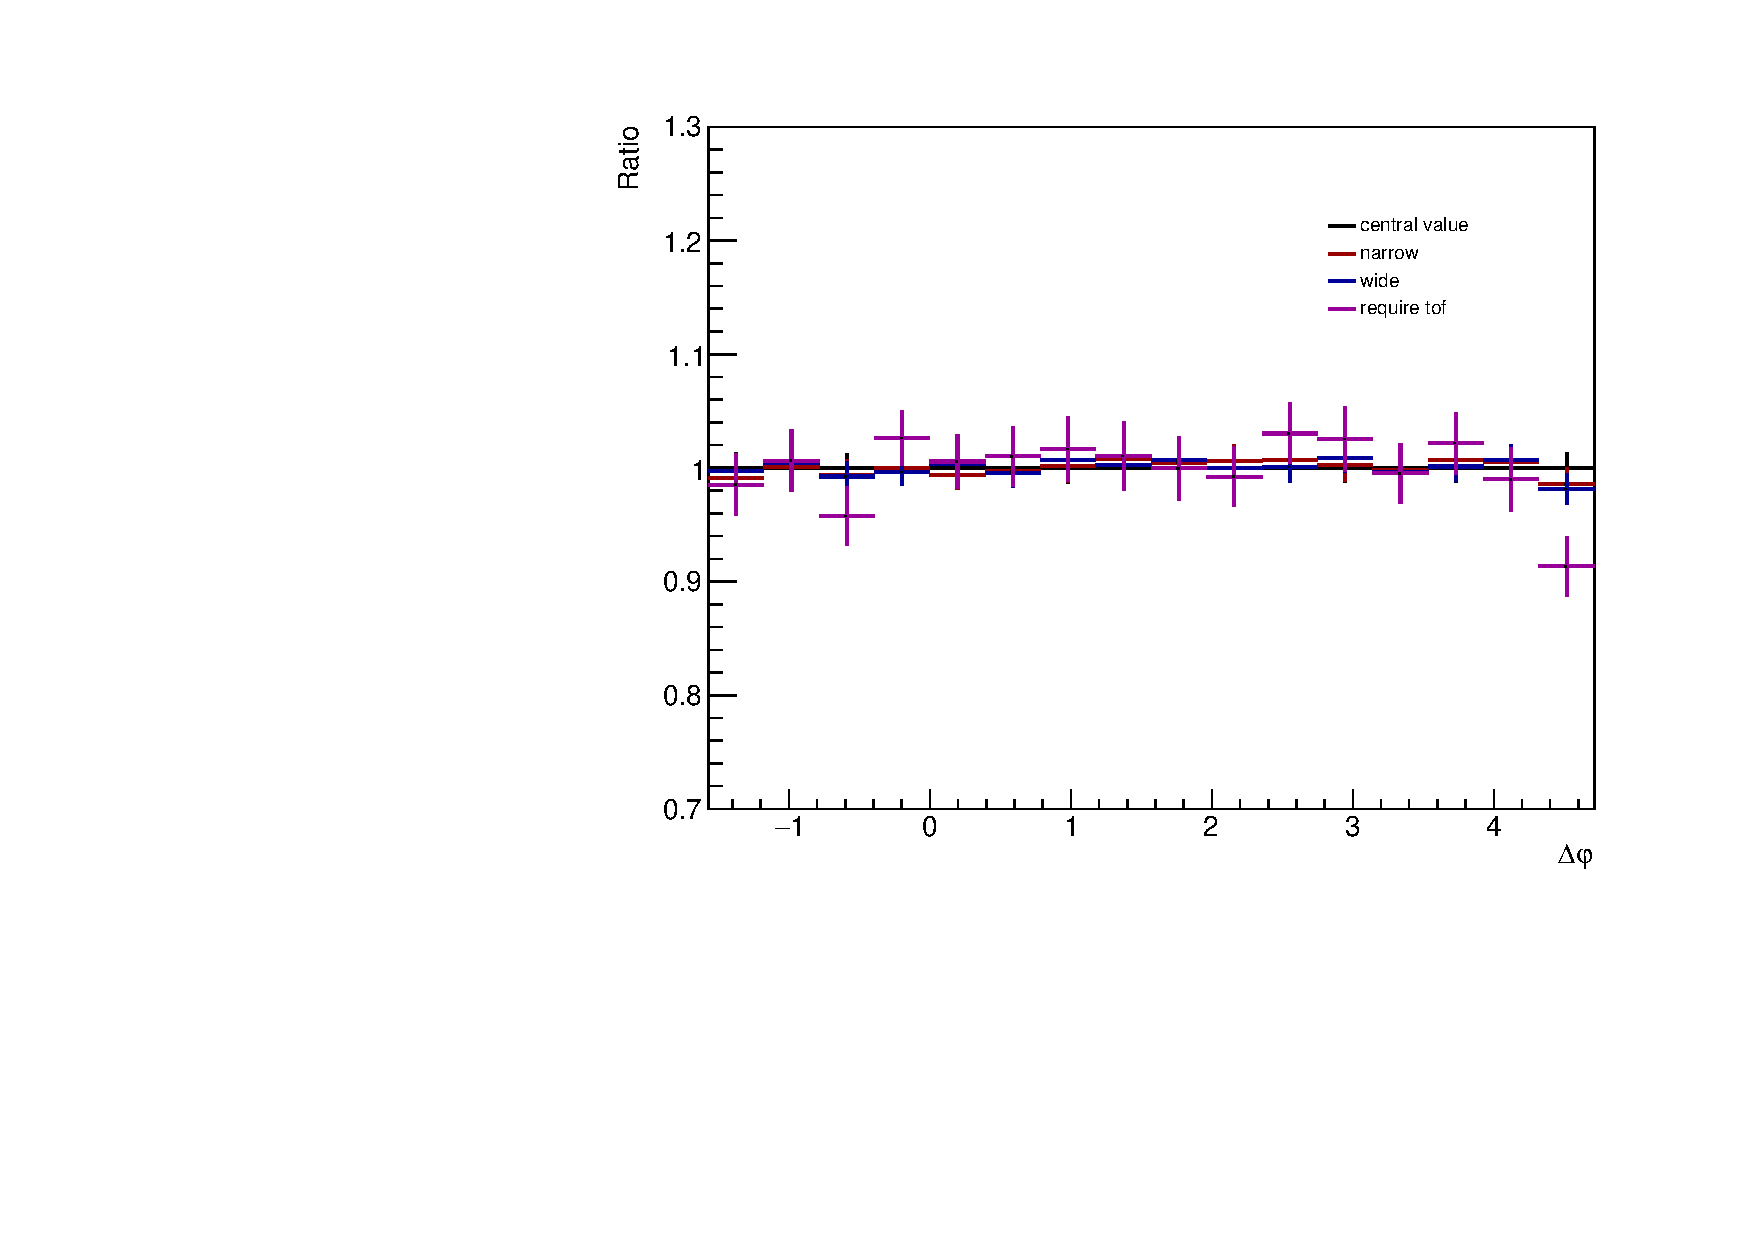
\includegraphics[width=0.49\textwidth]{figures/analysis/pid_variations_dphi_20_50_lowpt_ratio.pdf}
    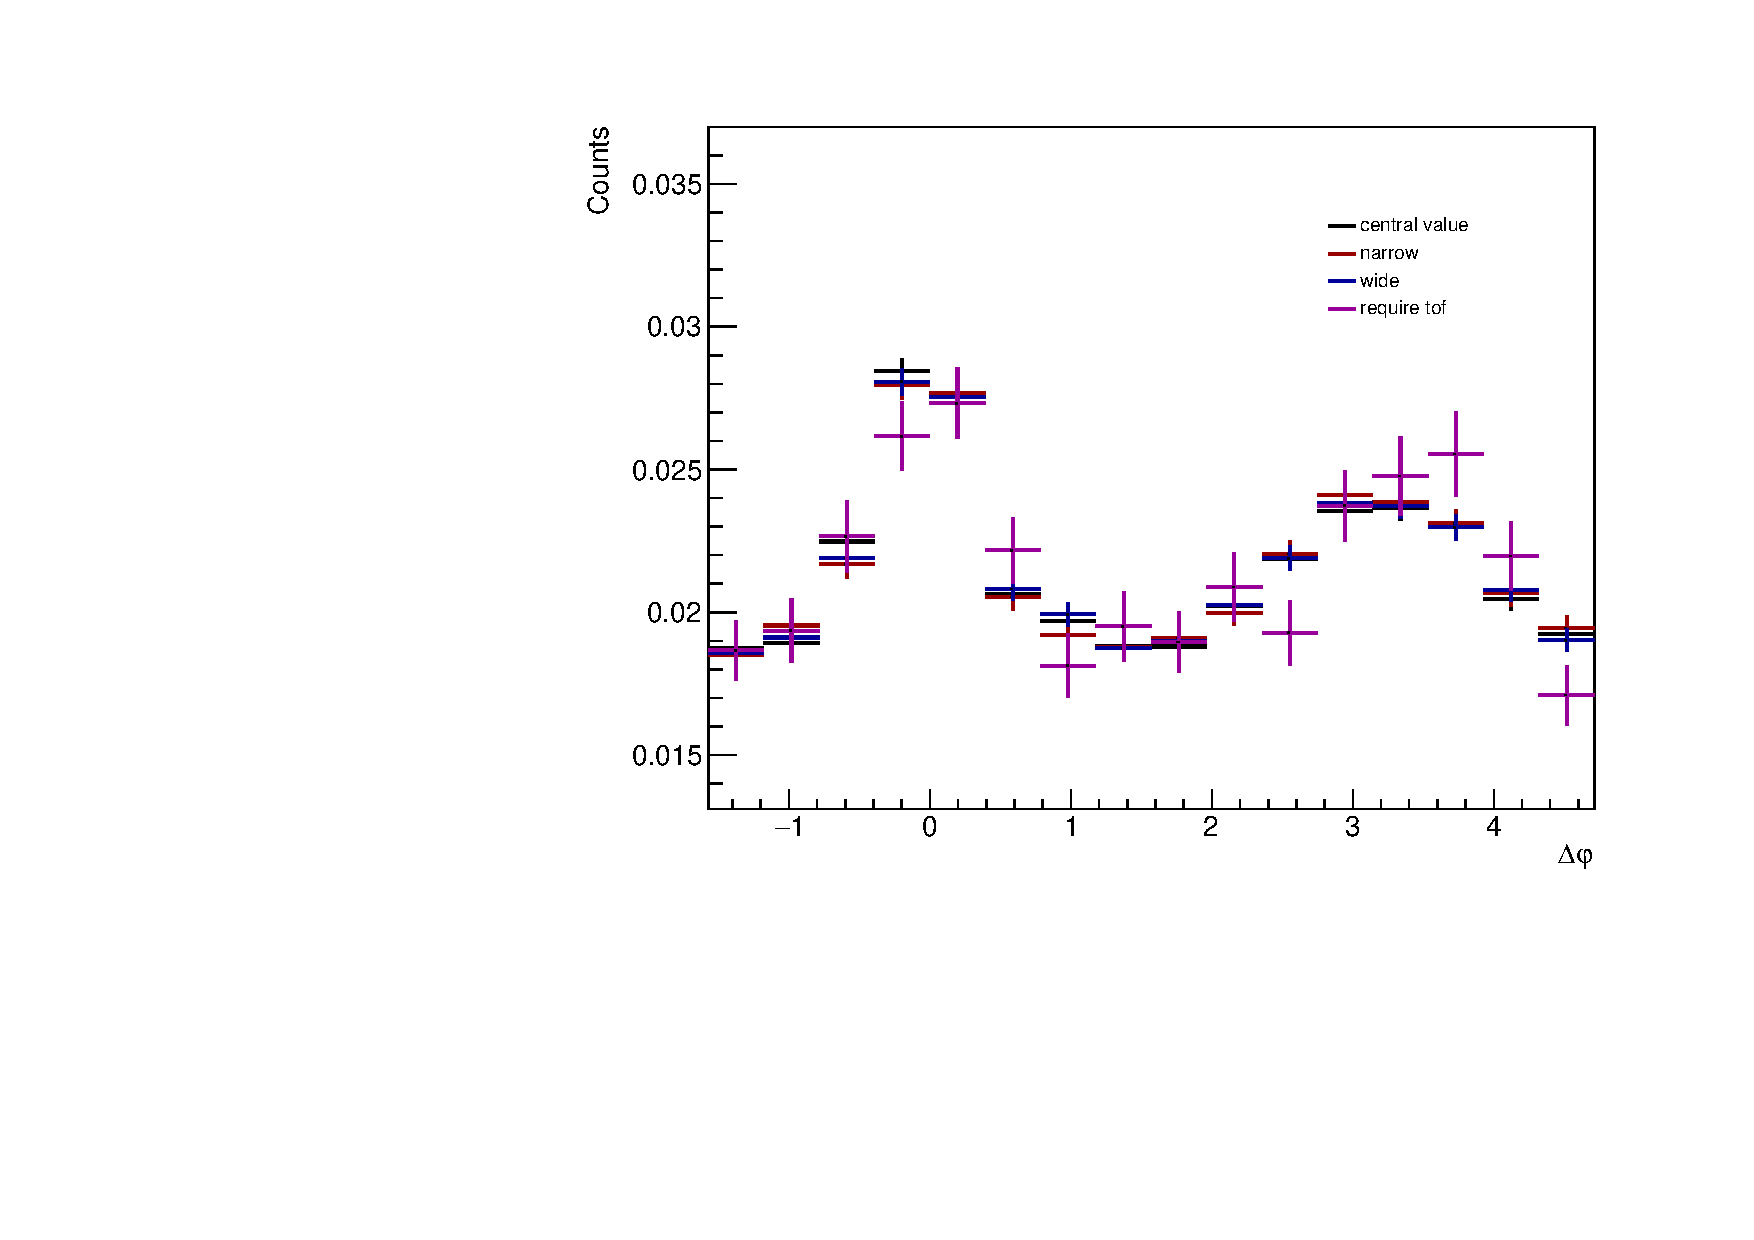
\includegraphics[width=0.49\textwidth]{figures/analysis/pid_variations_dphi_50_80_lowpt.pdf}
    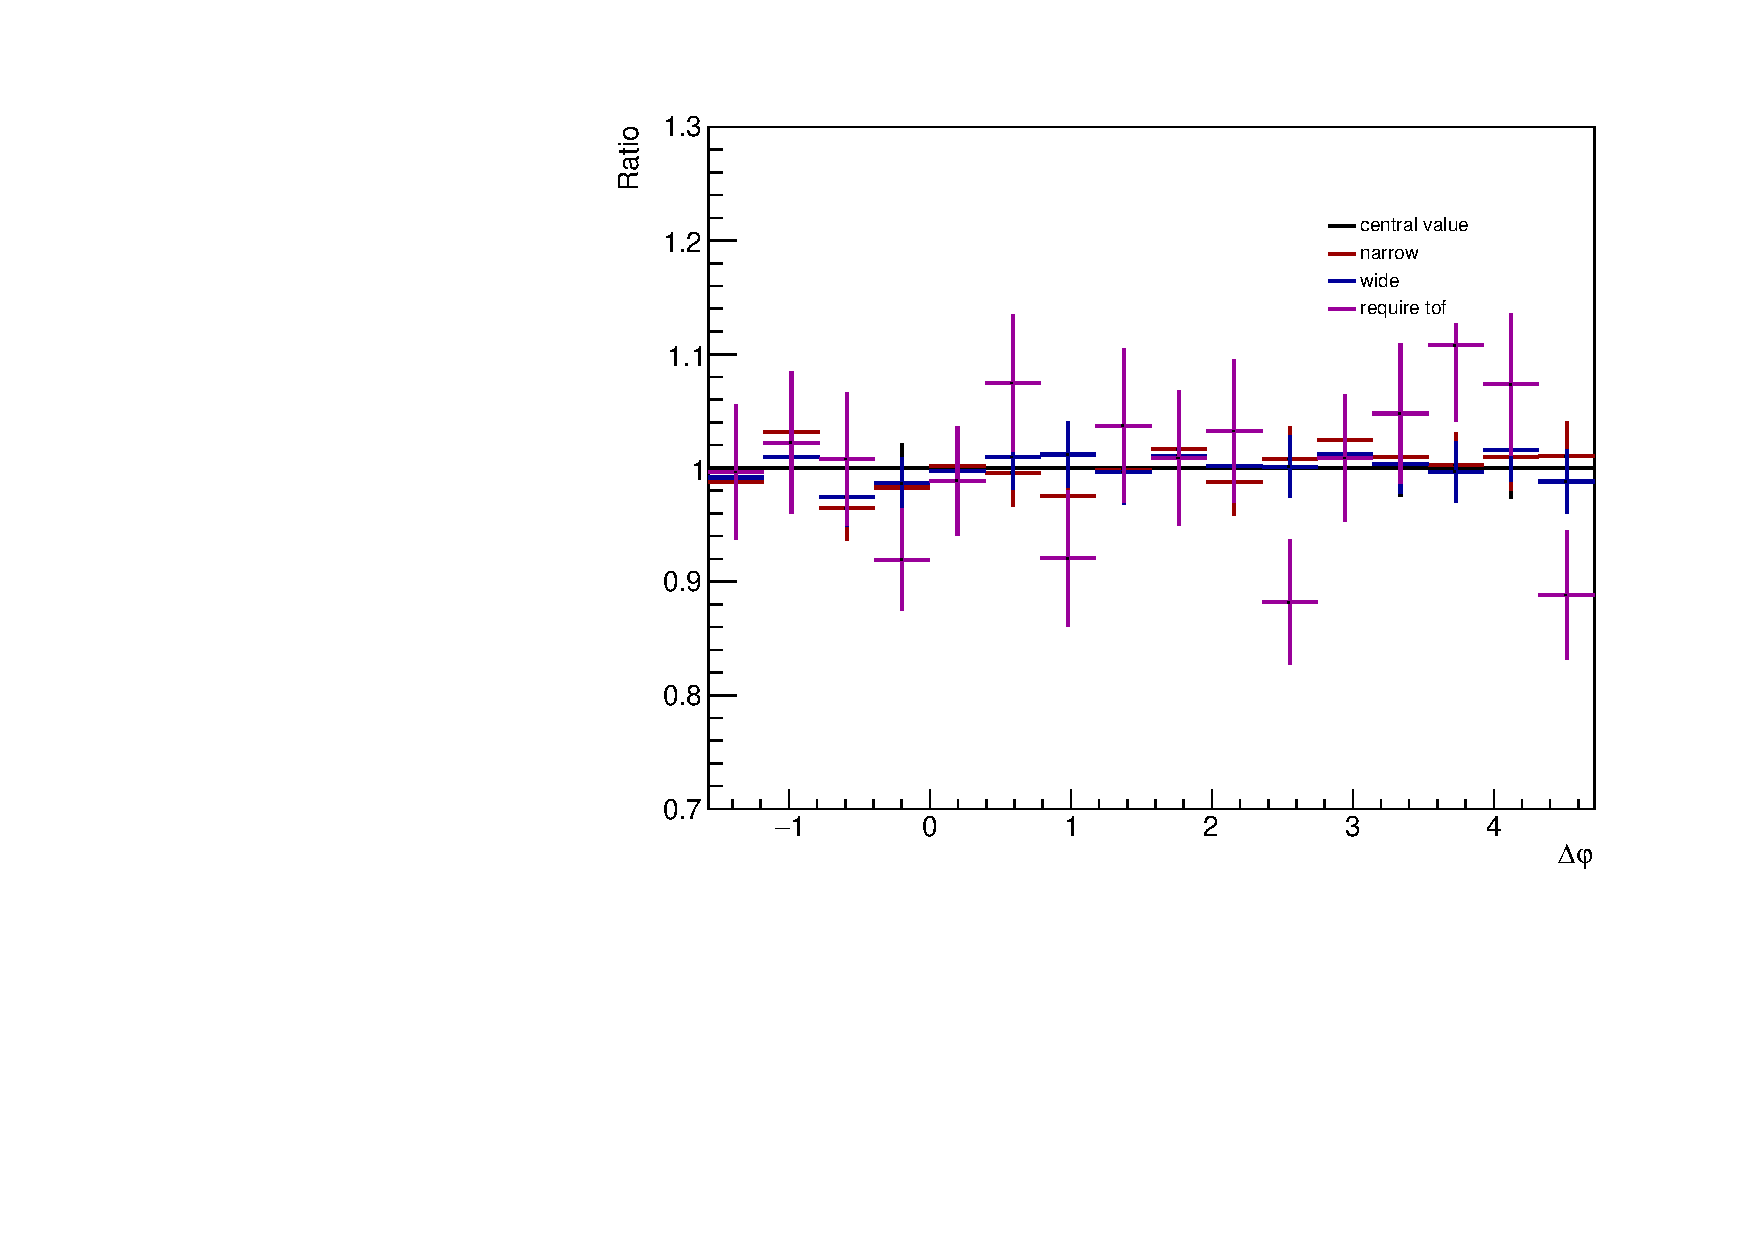
\includegraphics[width=0.49\textwidth]{figures/analysis/pid_variations_dphi_50_80_lowpt_ratio.pdf}
    \caption{The h-\lmb $\Delta\varphi$ distributions within the 0-20\% (top), 20-50\% (middle) and 50-80\% (bottom) multiplicity bins in the lower associated \pt bin for each of the PID cut variations (left) with the ratios to the nominal distribution (right).}
    \label{fig:pid_cut_variations_lowpt}
\end{figure}

\begin{figure}[ht]
    \centering
    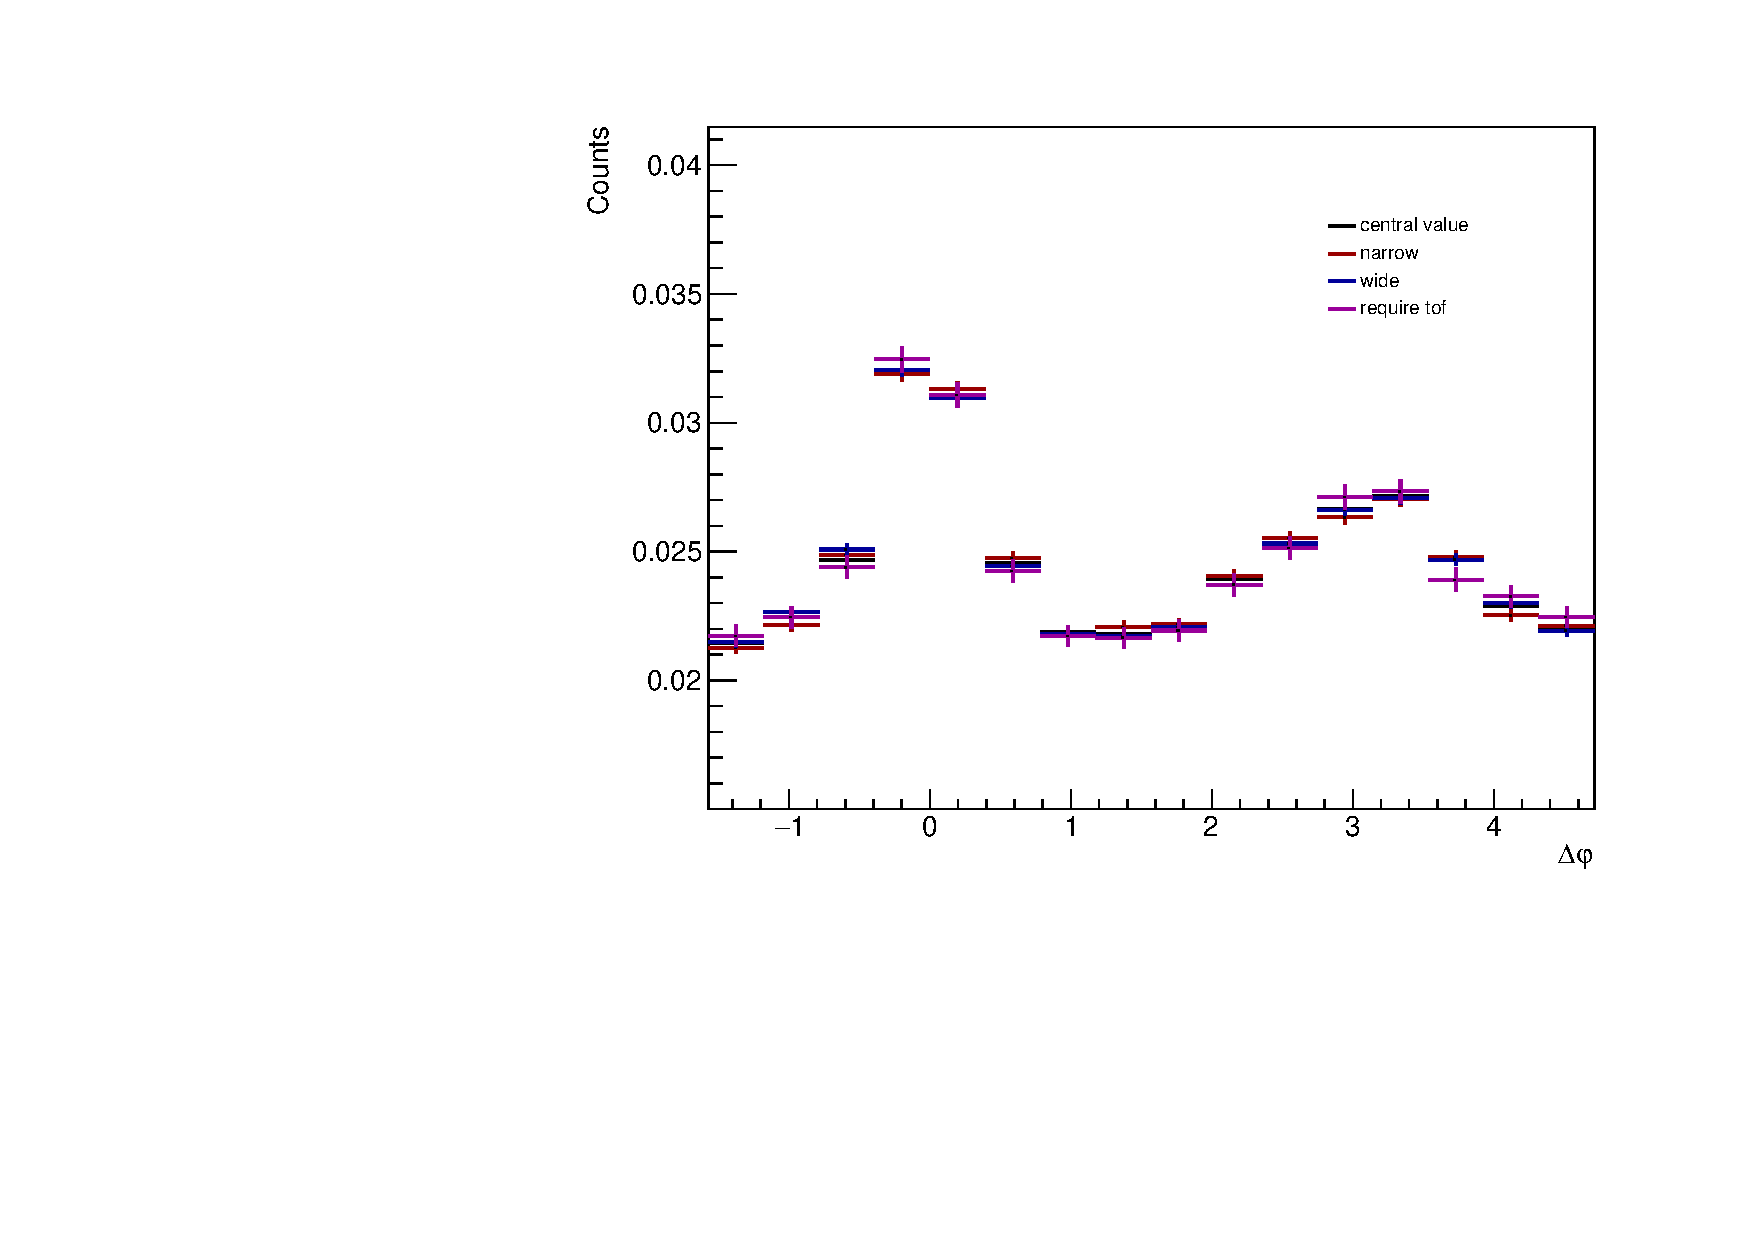
\includegraphics[width=0.49\textwidth]{figures/analysis/pid_variations_dphi_0_20_highpt.pdf}
    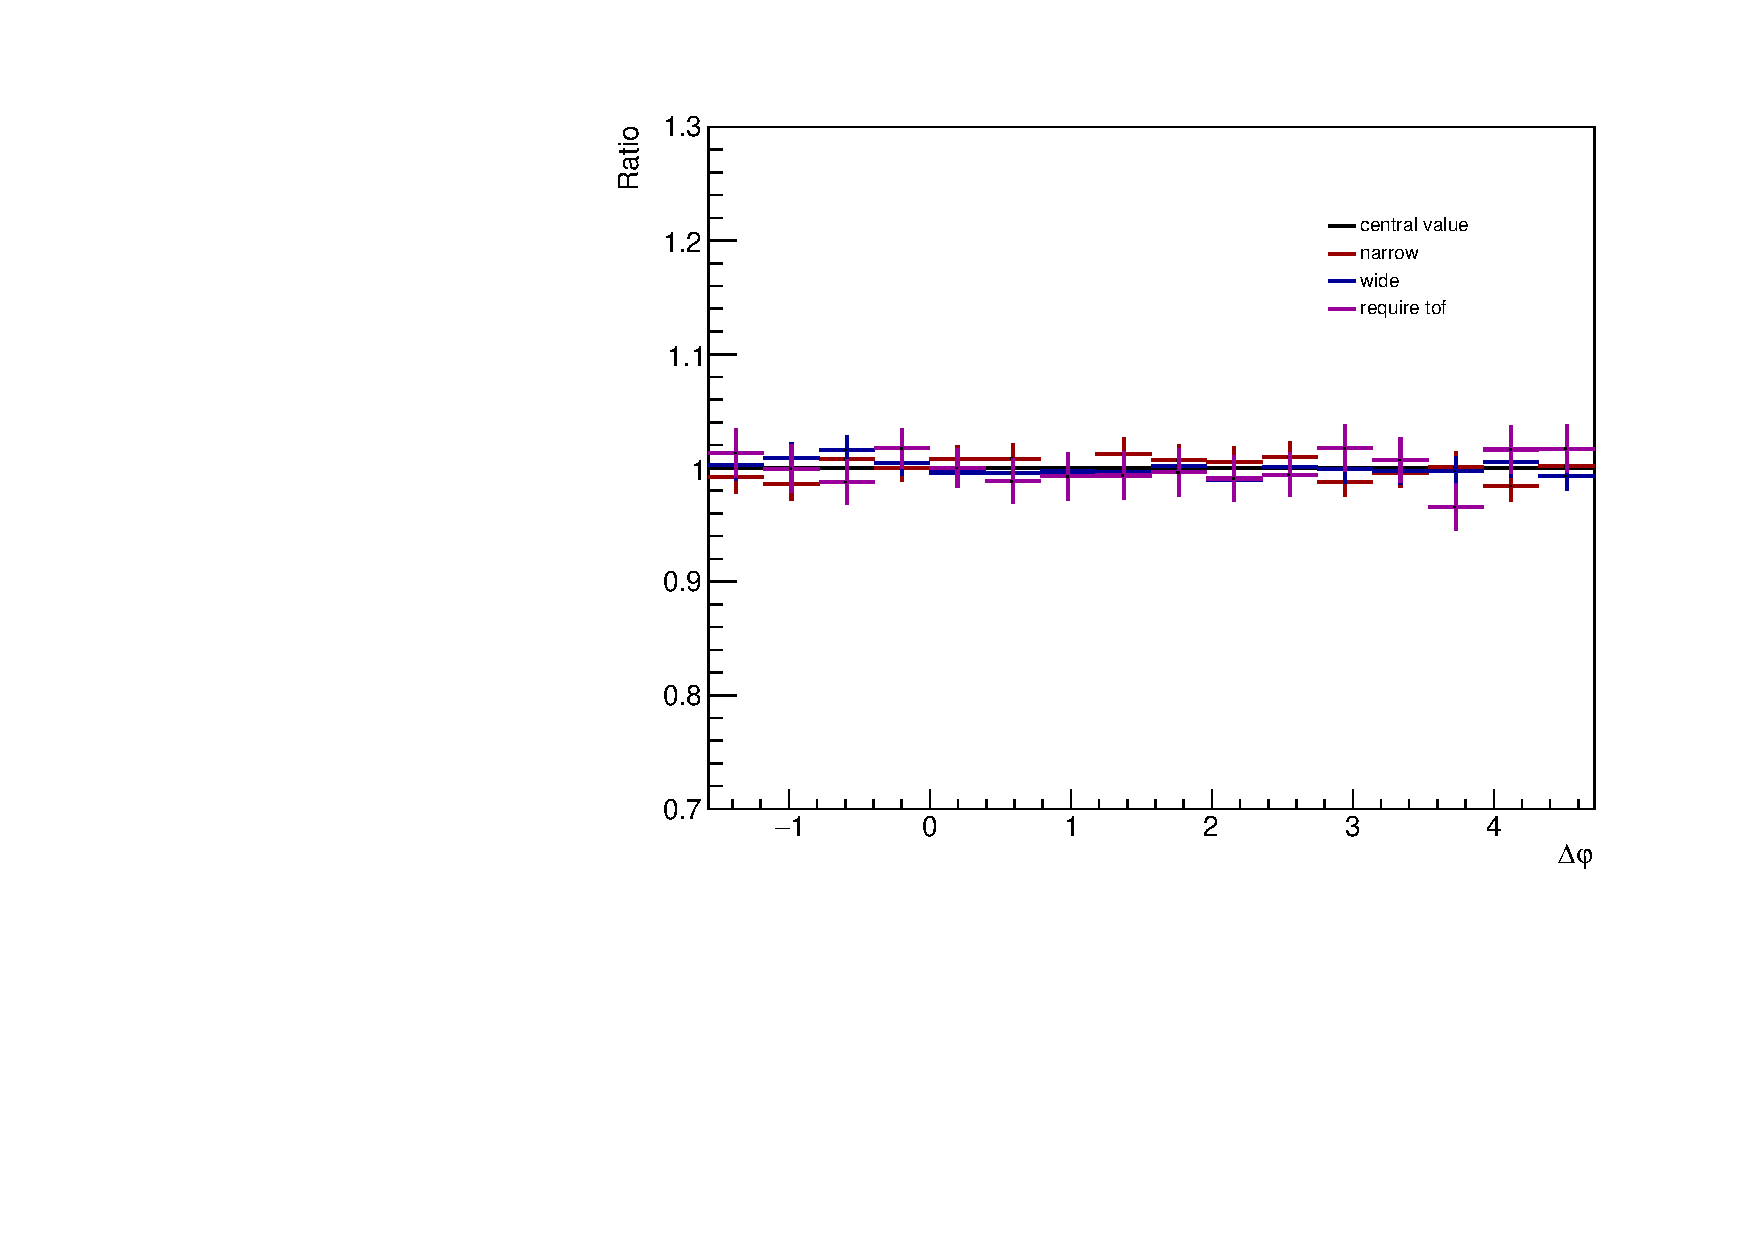
\includegraphics[width=0.49\textwidth]{figures/analysis/pid_variations_dphi_0_20_highpt_ratio.pdf}
    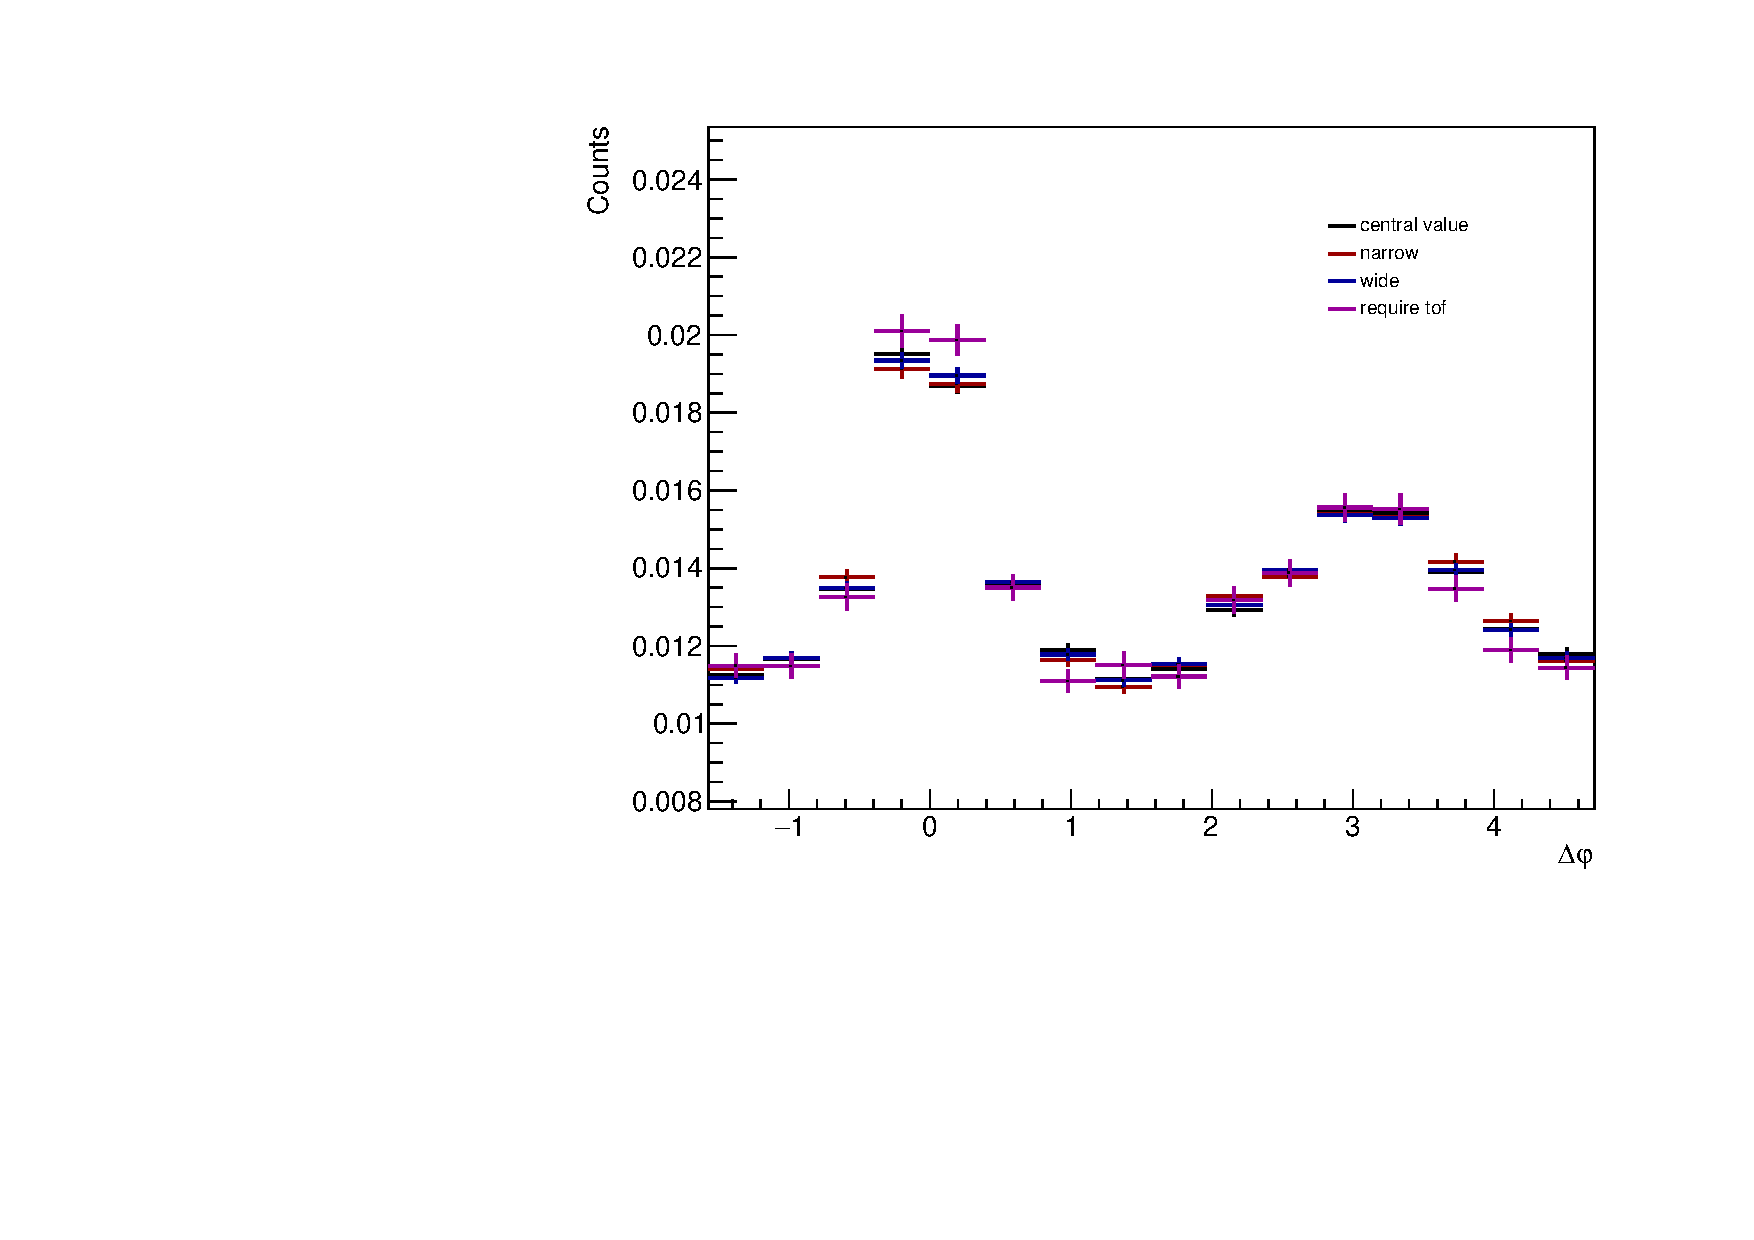
\includegraphics[width=0.49\textwidth]{figures/analysis/pid_variations_dphi_20_50_highpt.pdf}
    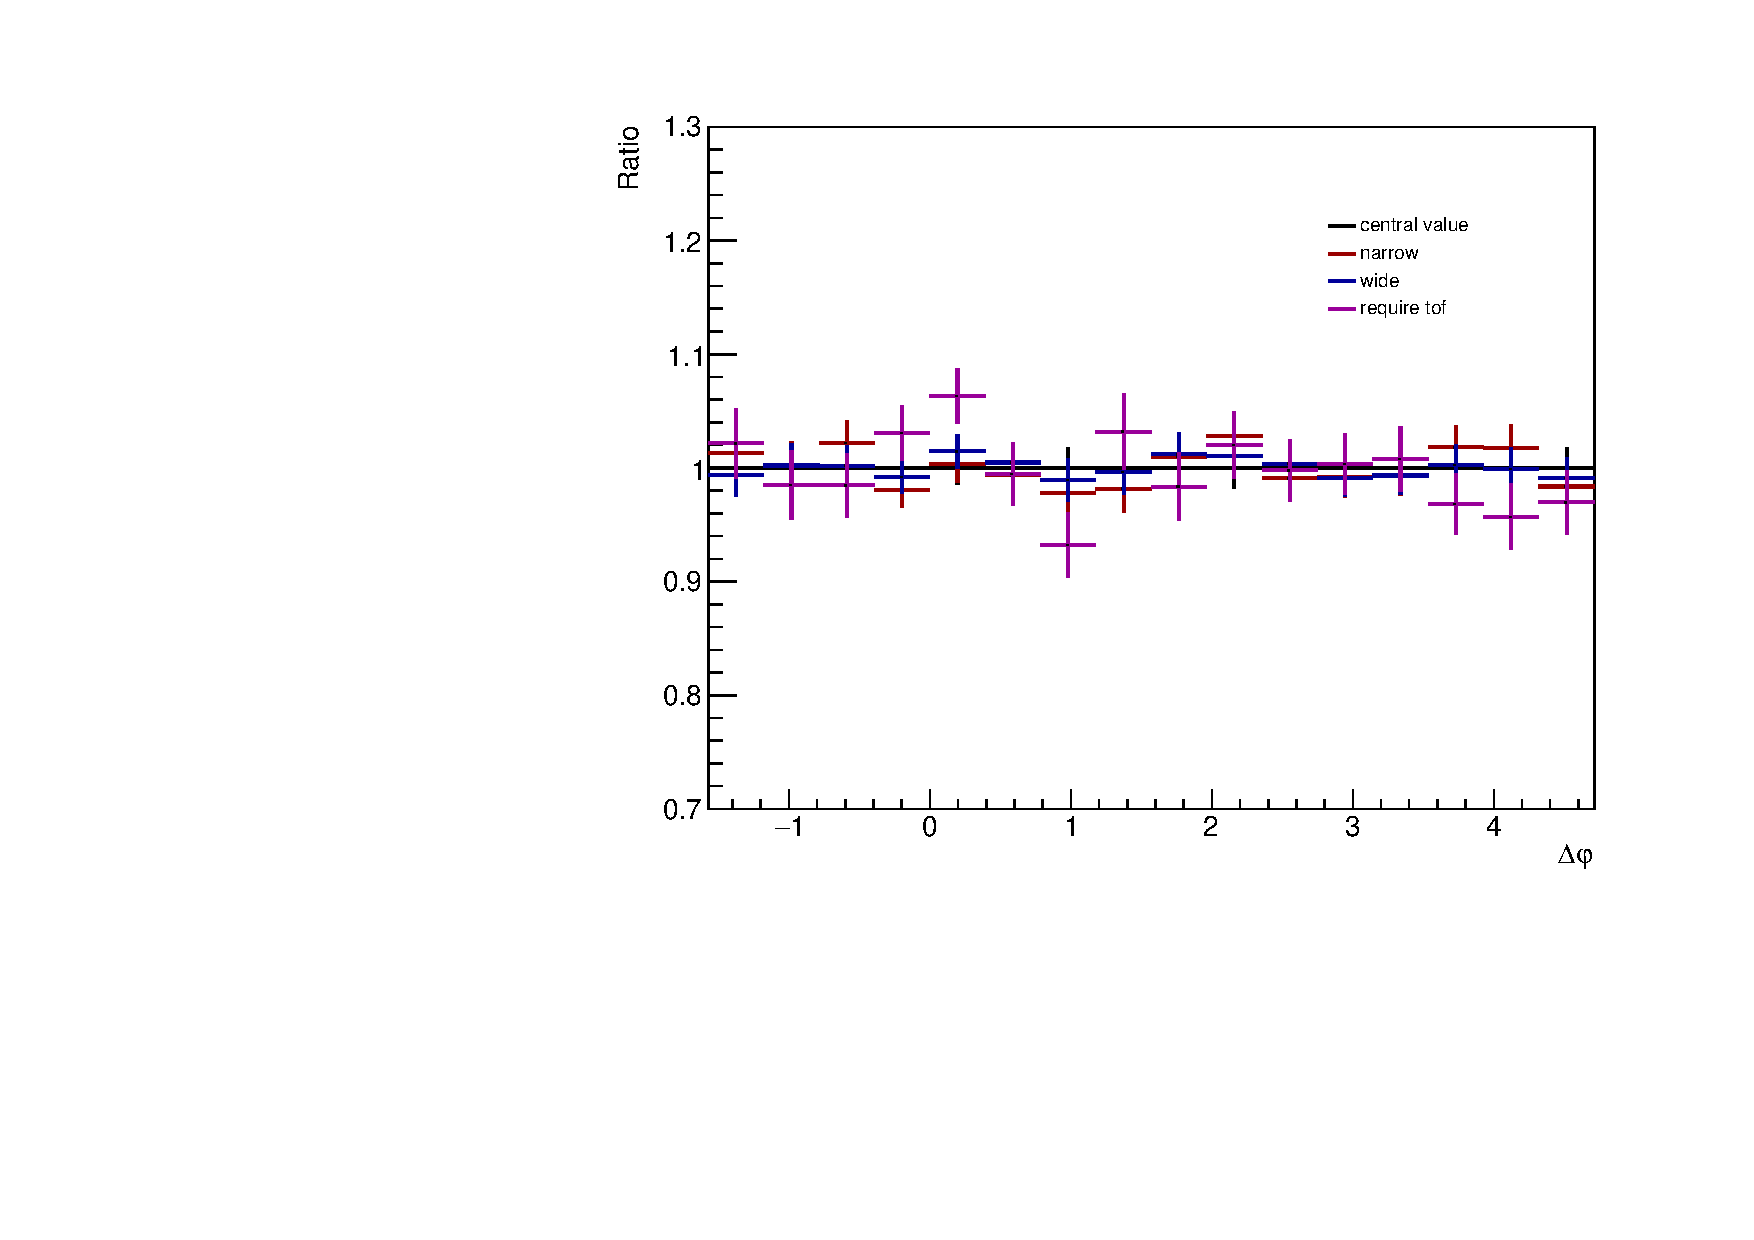
\includegraphics[width=0.49\textwidth]{figures/analysis/pid_variations_dphi_20_50_highpt_ratio.pdf}
    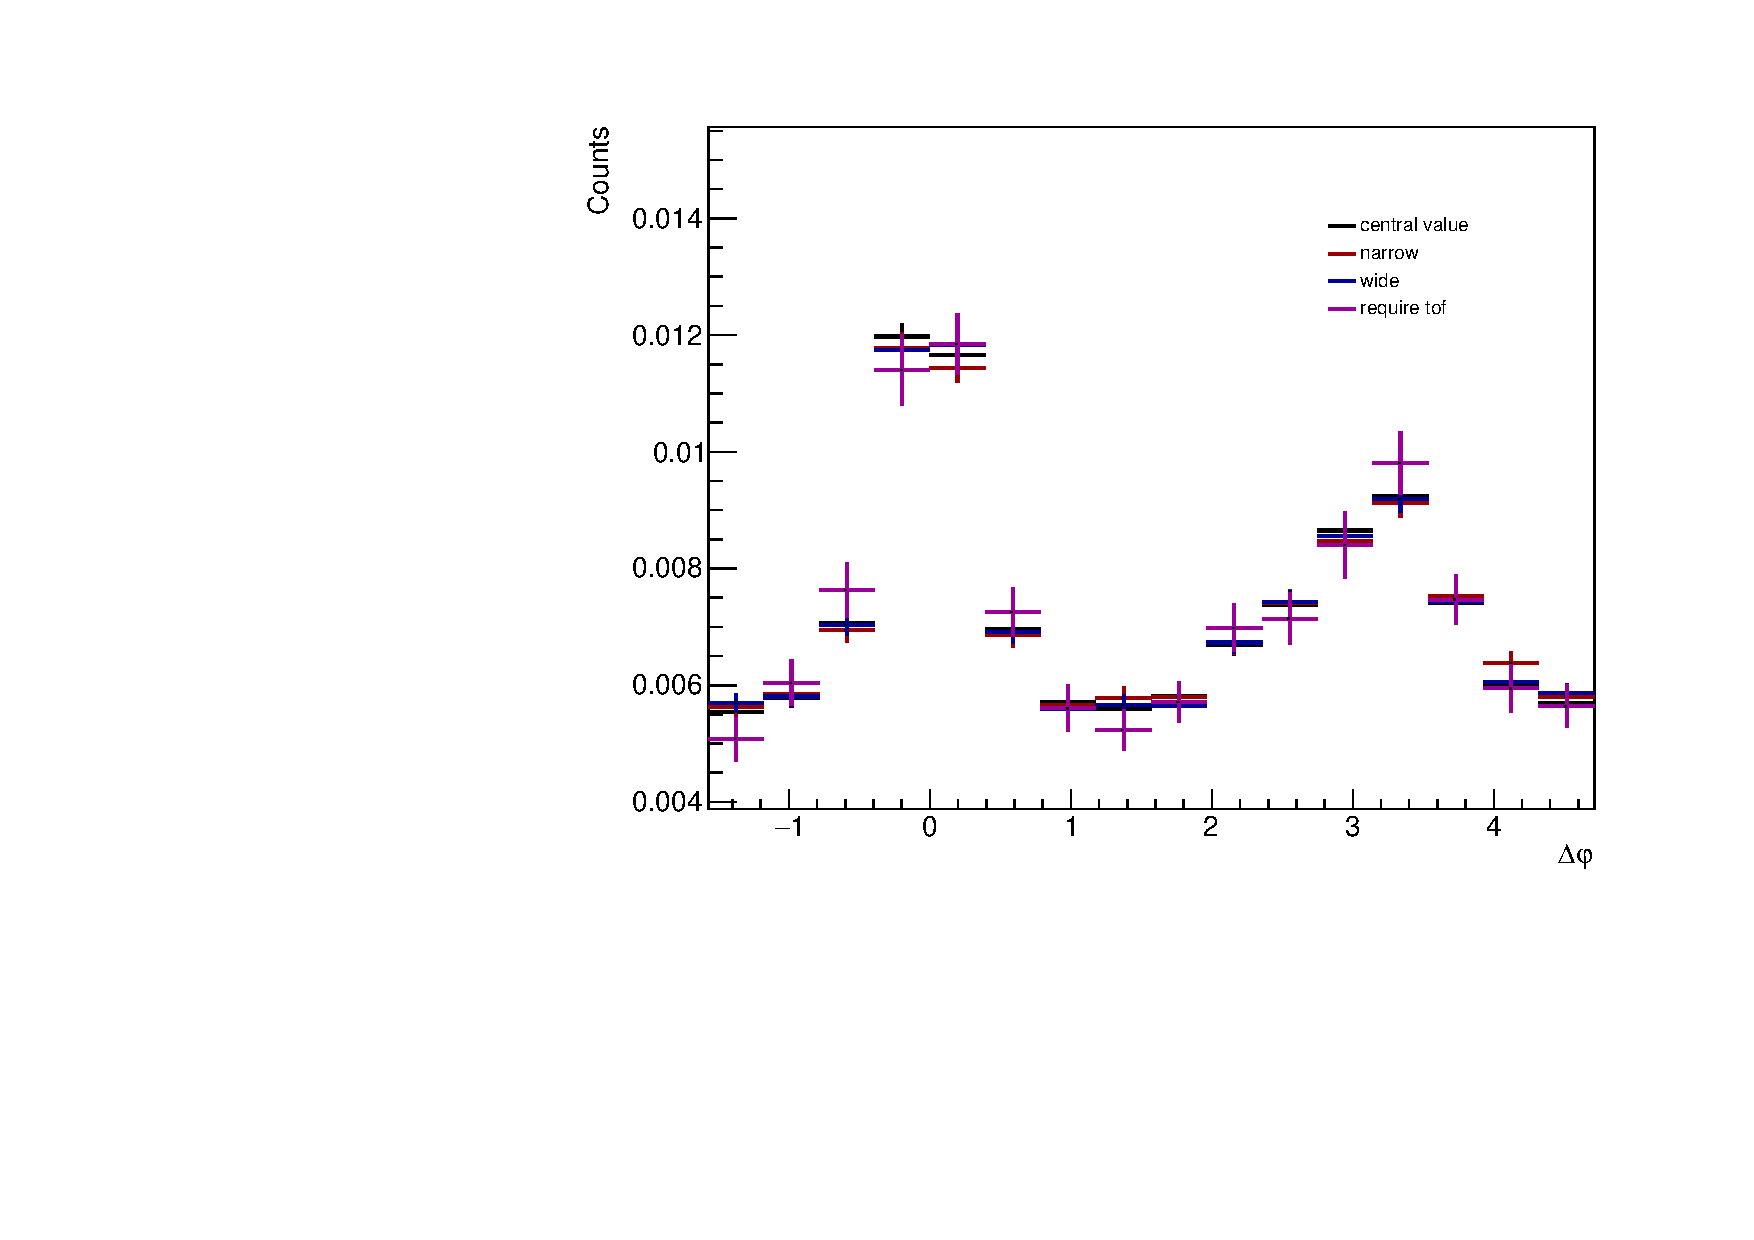
\includegraphics[width=0.49\textwidth]{figures/analysis/pid_variations_dphi_50_80_highpt.pdf}
    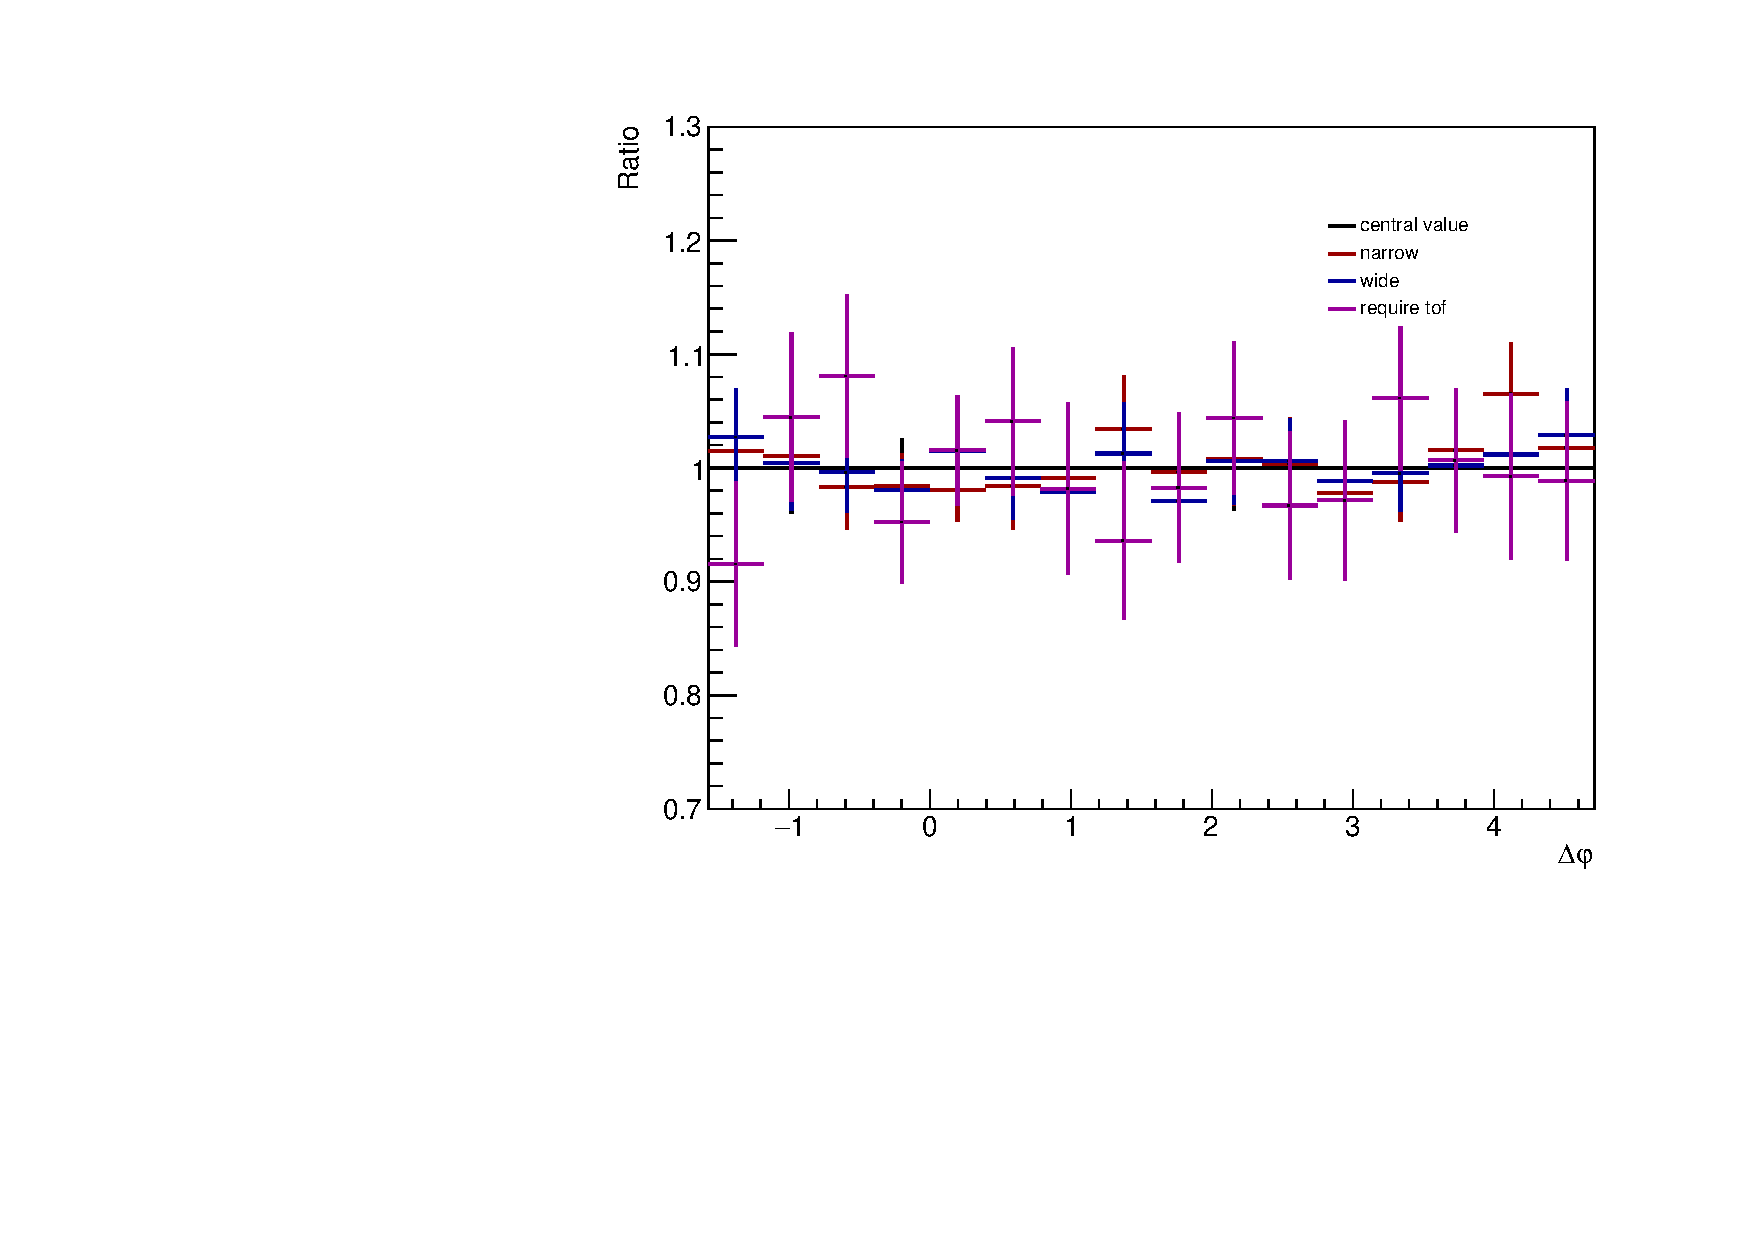
\includegraphics[width=0.49\textwidth]{figures/analysis/pid_variations_dphi_50_80_highpt_ratio.pdf}
    \caption{The h-\lmb $\Delta\varphi$ distributions within the 0-20\% (top), 20-50\% (middle) and 50-80\% (bottom) multiplicity bins in the higher associated \pt bin for each of the PID cut variations (left) with the ratios to the nominal distribution (right).}
    \label{fig:pid_cut_variations_highpt}
\end{figure}

\clearpage

\subsubsection{Barlow check for $\Delta\varphi$ distribution generation}
\label{sec:barlow_check_dphi}

Due to statistical fluctuations, it may be the case that some variations result in a statistically insignificant deviation from the nominal $\Delta\varphi$ distribution. In such cases, the variation should not be considered in the final systematic uncertainty calculation. To determine which variations give statistically significant deviations, a Barlow check~\cite{BarlowCheck} is performed. For each $\Delta\varphi$ bin, the following quantity is calculated:
%
\begin{equation}
    \label{eq:barlow_check}
	N\sigma_{RB} := \frac{y_{\text{var.}} - y_{\text{nom.}}}{\sqrt{|\sigma_{\text{var.}}^2 - \sigma_{\text{nom.}}^2|}},
\end{equation}
%
where $y_{\text{var.}}$ and $\sigma_{\text{var.}}$ are the measured yield and statistical uncertainty for the variation, and $y_{\text{nom.}}$ and $\sigma_{\text{nom.}}$ are the yield and statistical uncertainty for the nominal value. 

To determine whether a given variation should be excluded, the number $\Delta\varphi$ bins that have $|N\sigma_{RB}| < 1$ is counted. If this is the majority of the bins (across all multiplicity and associated \pt ranges),the variation is excluded from the systematic calculation. Example plots of $N\sigma_{RB}$ for each variation of the signal, sideband and PID cuts are shown in Figure \ref{fig:barlow_check_0_20}. The red lines represent $N\sigma_{RB} = \pm 1$.

\begin{figure}[ht]
    \centering
    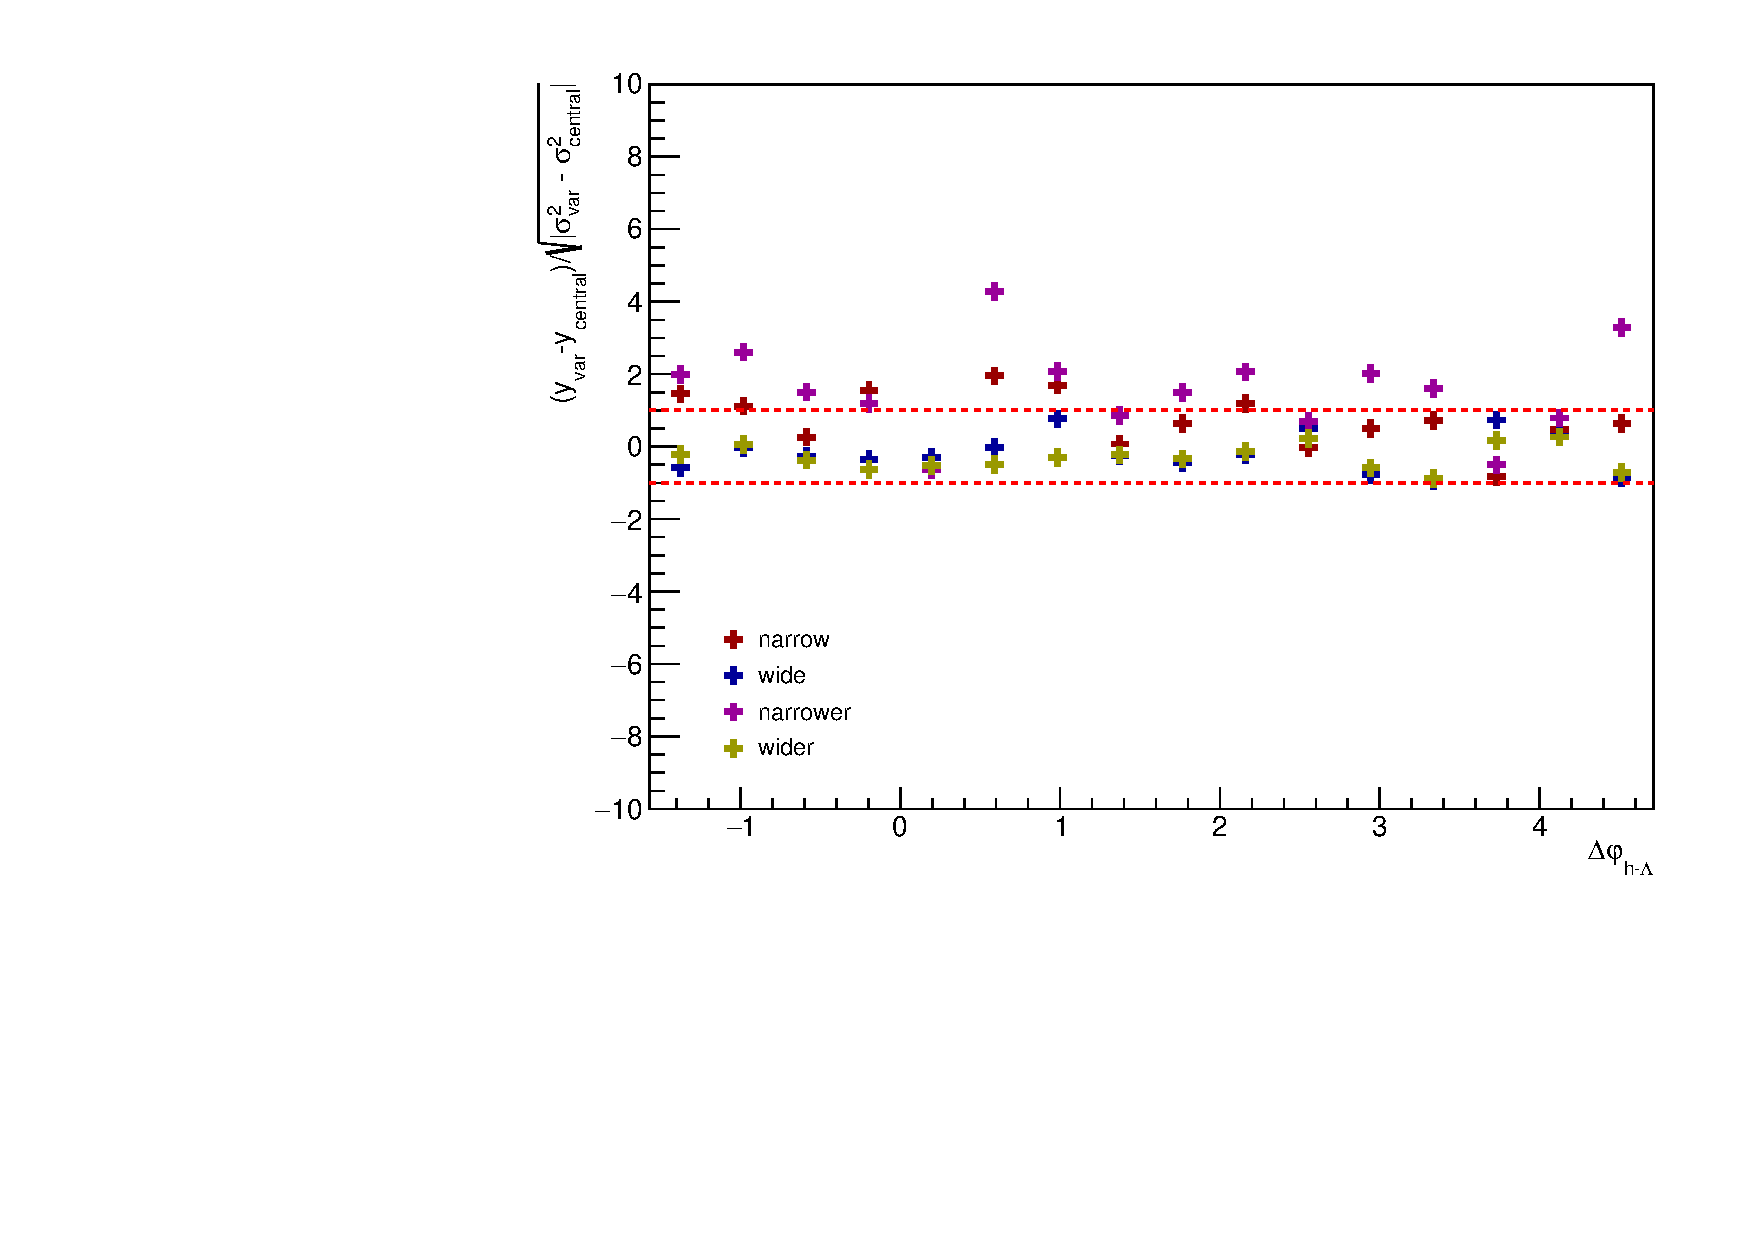
\includegraphics[width=0.32\textwidth]{figures/analysis/signal_barlow_0_20.pdf}
    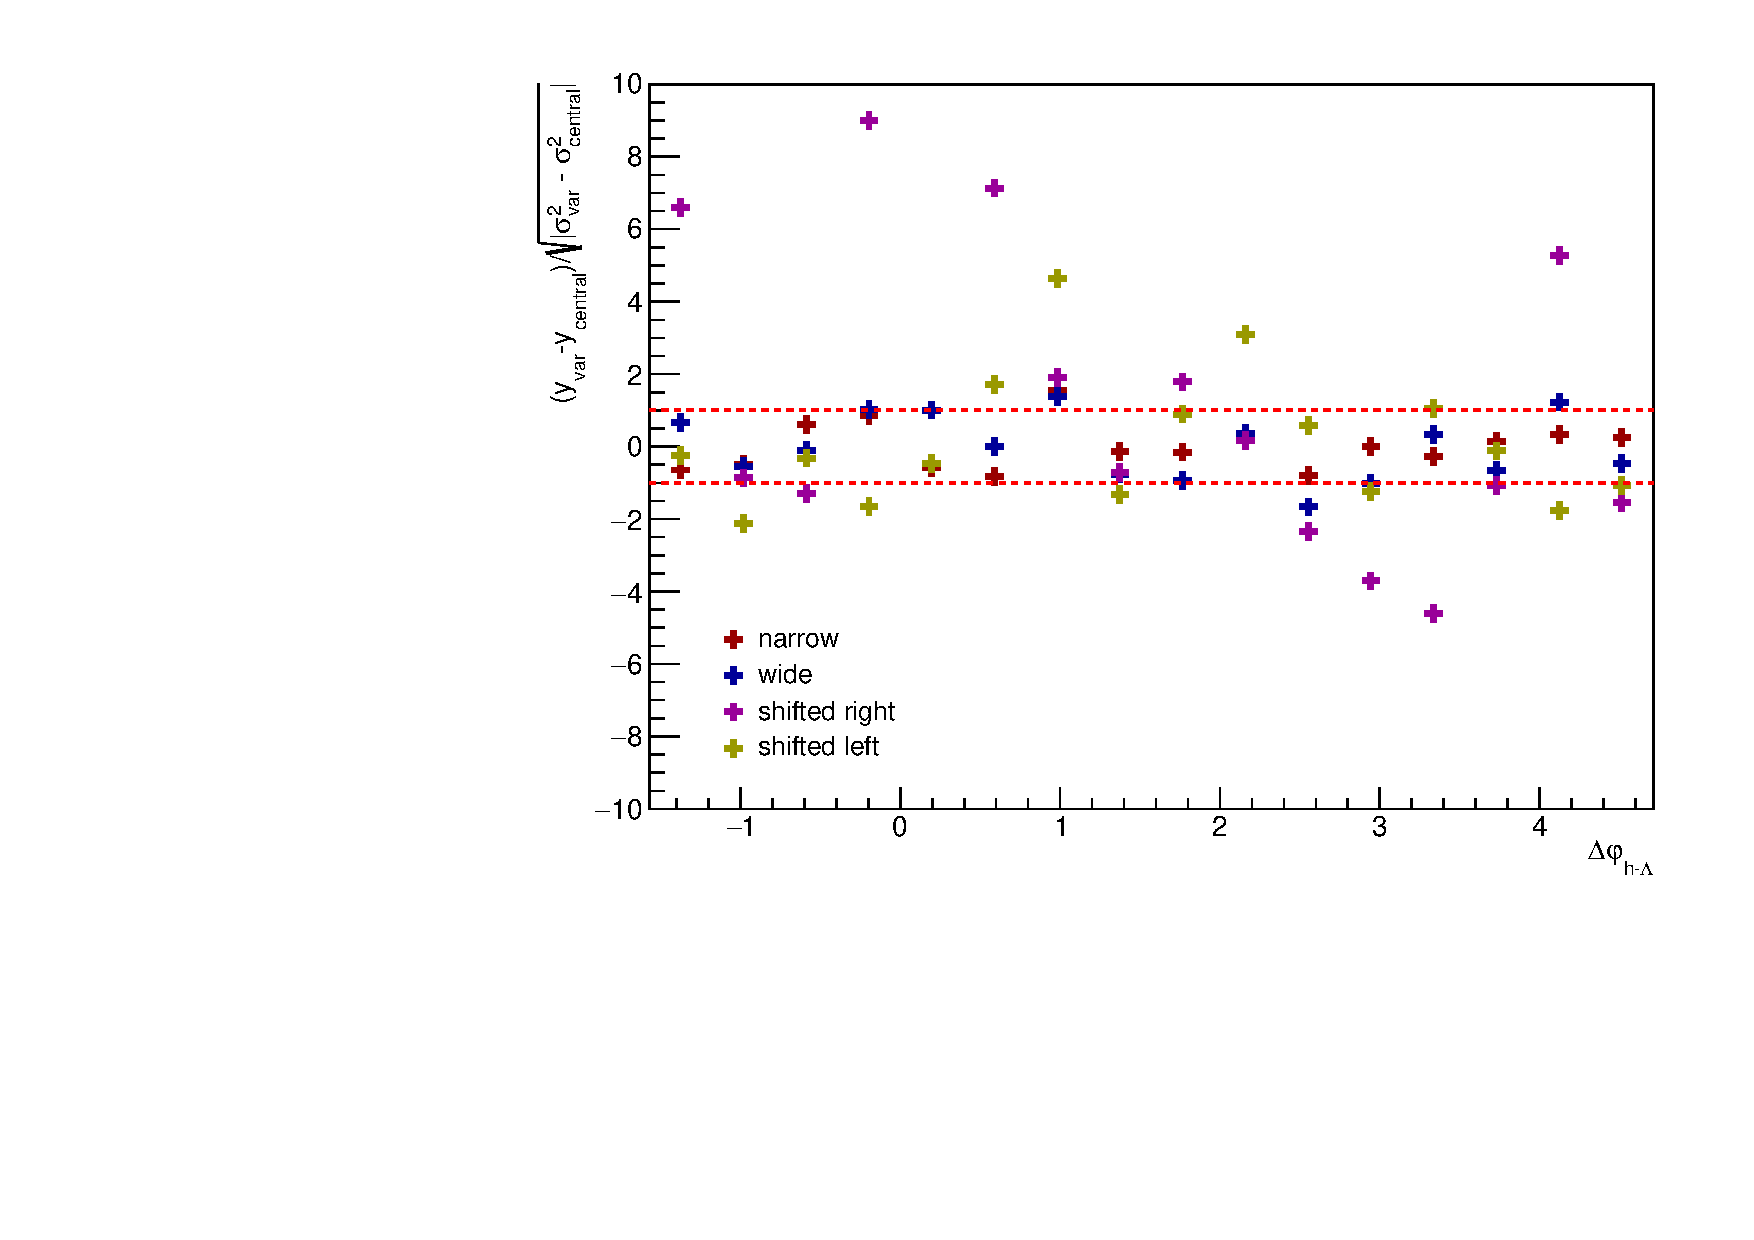
\includegraphics[width=0.32\textwidth]{figures/analysis/sideband_barlow_0_20.pdf}
    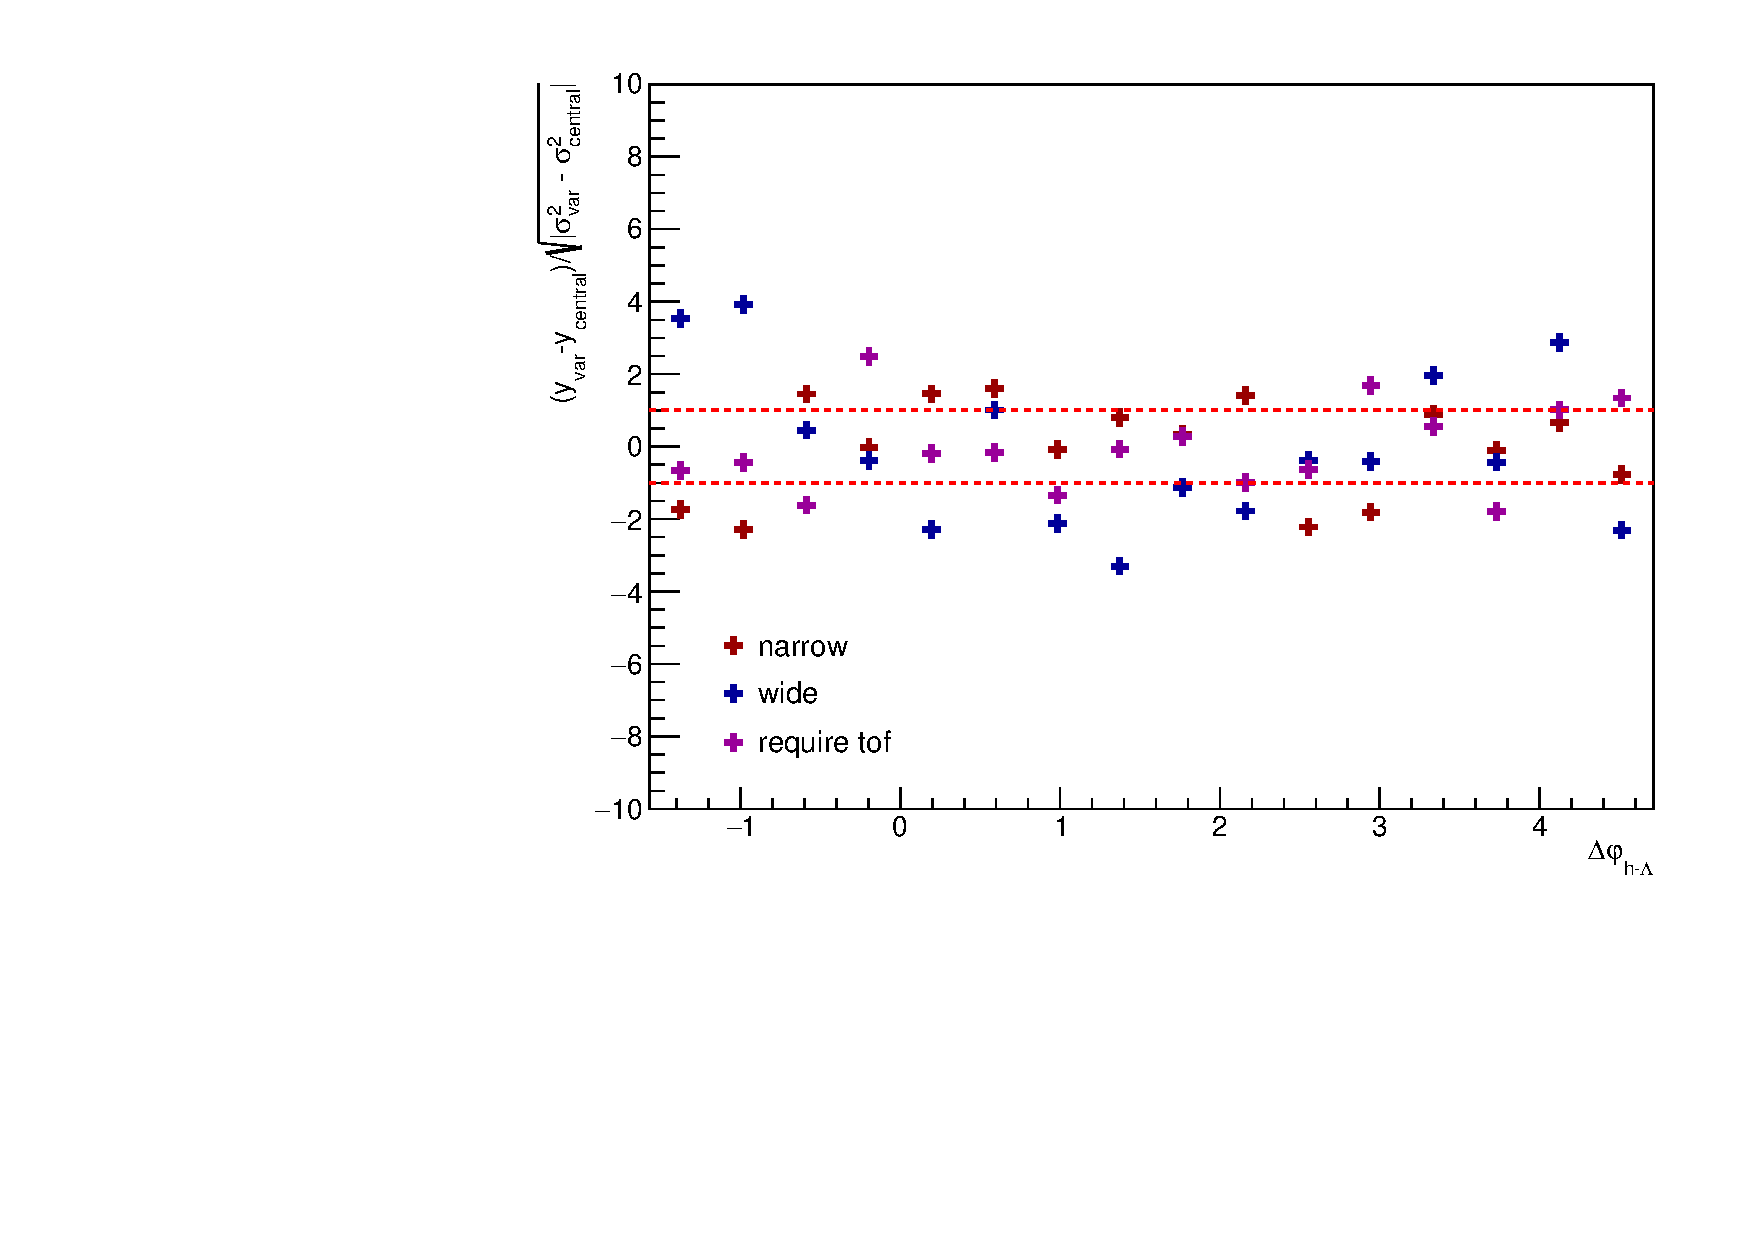
\includegraphics[width=0.32\textwidth]{figures/analysis/pid_barlow_0_20.pdf}
    \caption{Barlow check for the signal (left), sideband (middle), and PID (right) variations in the 0-20\% multiplicity bin. The red lines represent $N\sigma_{RB} = \pm 1$, and if the majority of the points fall within the red lines (across all $\Delta\varphi$, multiplicty and \pt bins), they are excluded from the systematic uncertainty calculation.}
    \label{fig:barlow_check_0_20}
\end{figure}

As a result of the check, the following variations are excluded from the final systematic uncertainty calculation:
%
\begin{itemize}
    \item Signal: wide, wider
    \item Sideband: wide, narrow
    \item PID: require TOF
\end{itemize}
%
These exclusions are not so surprising. As the nominal signal region is already fairly wide, making it wider does not significantly change the $\Delta\varphi$ distribution. Similarly, the initial sideband region falls fairly close to the signal region. So long as there are enough statistics in the corresponding sideband h-$\Lambda$ distribution, changing its width should not affect the $\Delta\varphi$ distribution in a meaningful way. It also appears that requiring a TOF hit introduces large statistical errors, which dominate the denominator in Equation~\ref{eq:barlow_check}.

\subsubsection{$\Delta\varphi$ distribution systematics, summarized}
\label{sec:dphi_systematics_summarized}

The final systematic errors (after the Barlow check) from the h-\lmb $\Delta\varphi$ distribution generation for each multiplicity bin and \pt bin are shown in Table \ref{tab:h_lambda_dphi_systematics_table}. The total systematic uncertainty is calculated by adding each systematic error in quadrature. This table is consolidated into plots showing the systematic errors for each multiplicity bin and \pt bin, which are presented in Figure \ref{fig:dphi_systematics_plots}. As the systematic uncertainties associated with the generation of the dihadron $\Delta\varphi$ distributions are only from the tracking efficiency presented in Table~\ref{tab:flat_systematics}, they are not plotted in this section.

\begin{table}[ht]
    \centering
    \caption{The final systematic uncertainties (in percentages) from the h-$\Lambda$ $\Delta\varphi$ distribution generation for each multiplicity and associated \pt bin.}
    \label{tab:h_lambda_dphi_systematics_table}
    \begin{tabular}{l c c c c c c}
        \hline
        Mult. and \pt bin & Sig. & Sideband & PID & Topo. sel.  & Mat. bud. & Total \\
        \hline
        \hline
        0-20\%, low \pt & 0.36 & 0.53 & 0.64 & 3.2 & 1.1 & 3.3 \\
        20-50\%, low \pt & 0.35 & 0.67 & 0.65 & 3.2  & 1.1 & 3.4 \\
        50-80\%, low \pt & 0.76 & 1.1 & 1.4 & 3.2  & 1.1 & 3.8 \\
        0-20\%, high \pt & 0.42 & 0.42 & 0.76 & 3.0 & 0.6 & 3.2 \\
        20-50\%, high \pt & 0.4 & 0.71 & 1.2 & 3.0  & 0.6 & 3.3 \\
        50-80\%, high \pt & 1.1 & 1.6 & 2.0 & 3.0  & 0.6 & 4.1 \\
        \hline
    \end{tabular}
\end{table}


\begin{figure}[ht]
    \centering
    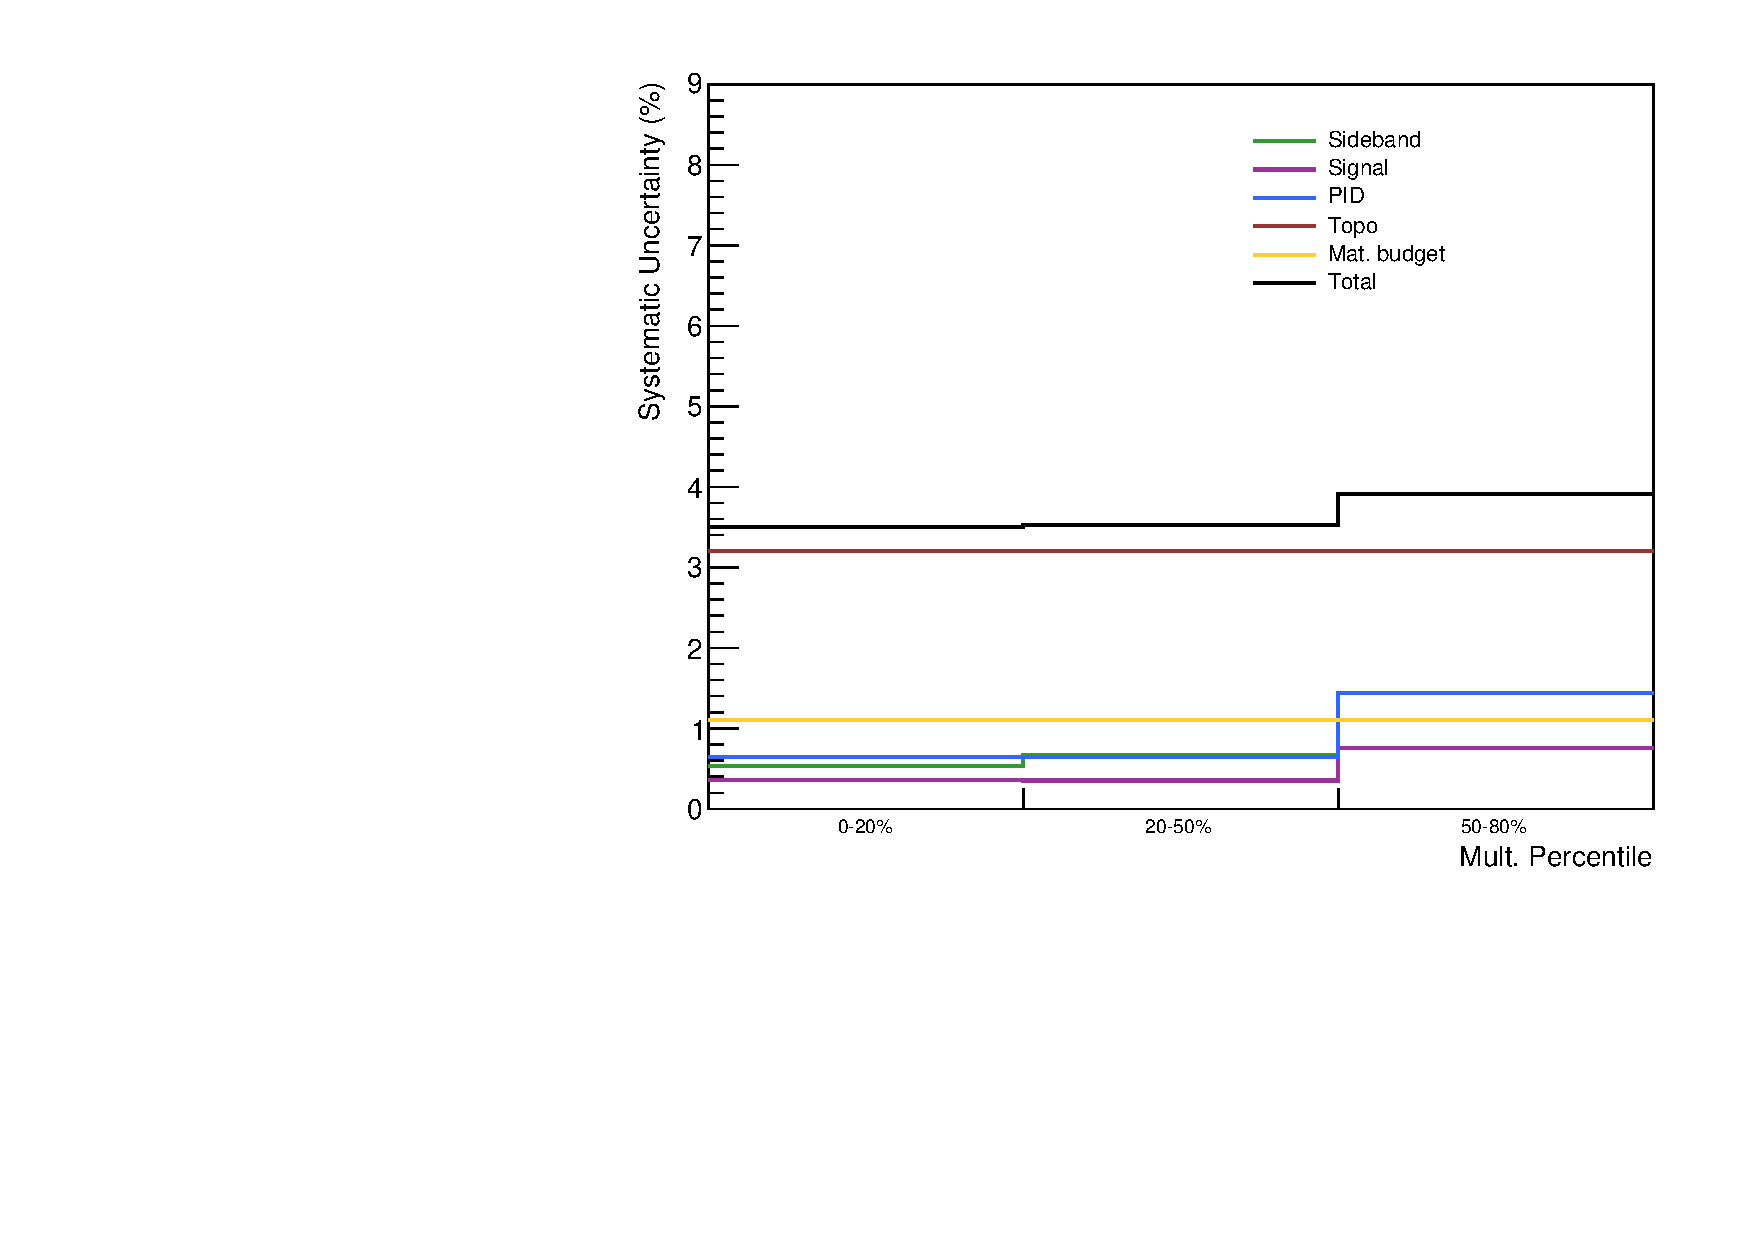
\includegraphics[width=0.48\textwidth]{figures/analysis/systematics_dphi_postbarlow_lowpt.pdf}
    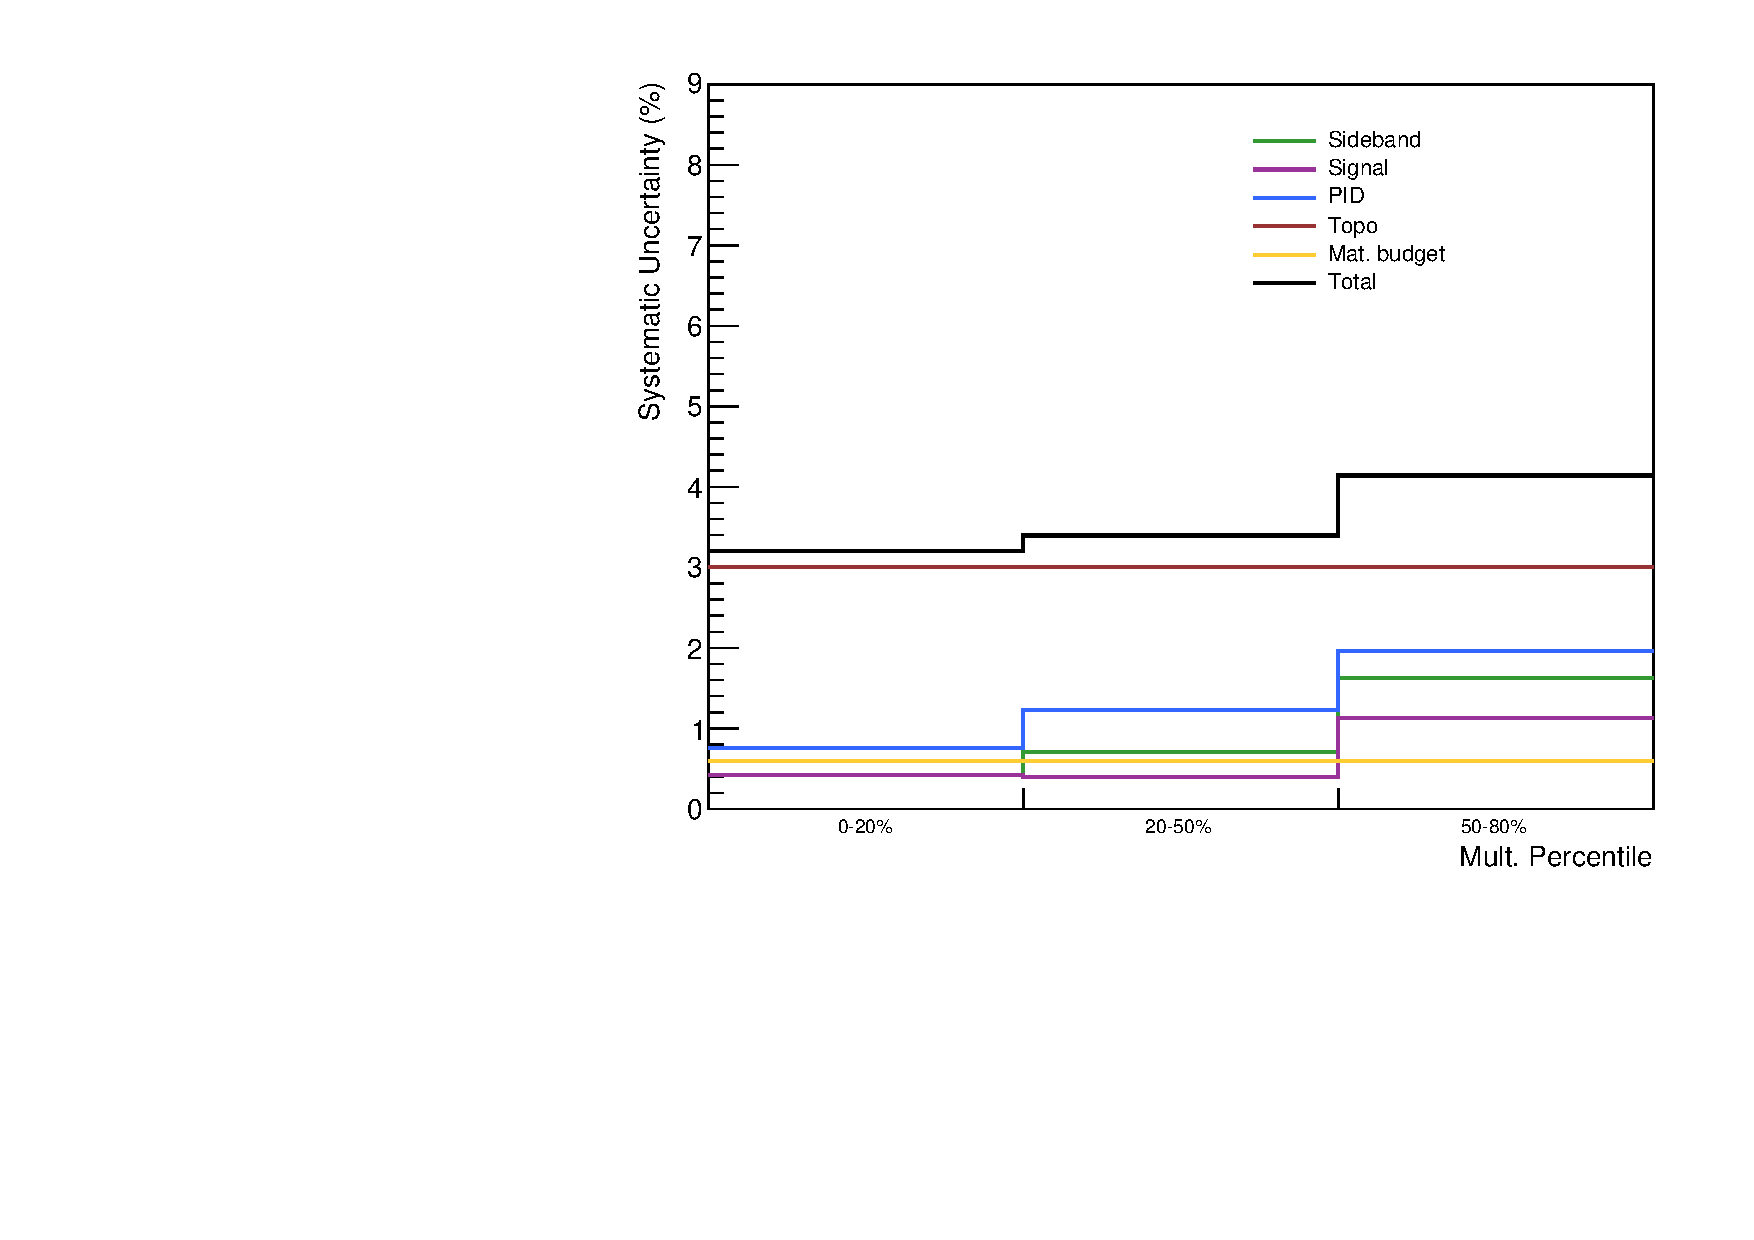
\includegraphics[width=0.48\textwidth]{figures/analysis/systematics_dphi_postbarlow_highpt.pdf}
    \caption{A visual depiction of the final systematic errors for the h-$\Lambda$ $\Delta\varphi$ distributions for each multiplicity bin in the low (left) and high (right) associated \pt bins. The total systematic error is shown in black.}
    \label{fig:dphi_systematics_plots}
\end{figure}

The total systematic error is observed to be mostly $p_{T}$-independent. However, there appears to be a slight correlation between the systematic uncertainty and multiplicity, with the 0-20\% bin exhibiting lower uncertainties than the 50-80\% bin across both \pt ranges. This can become problematic when investigating the multiplicity dependence of observables extracted from the $\Delta\varphi$ distributions, as the fraction of the systematic uncertainty which is directly correlated with multiplicity should not be considered when measuring multiplicity-dependent trends like slopes and percent changes. Because of this, the fraction of the systematic uncertainty which is uncorrelated with multiplicity is approximated using
%
\begin{equation}
    \label{eq:uncorrelated_fraction_1}
    \sigma_{\text{uncor}, i}^2 = \sum_{\text{vars}}(R_{\text{var}, i} - 1)^2,
\end{equation}
where 
\begin{equation}
    \label{eq:uncorrelated_fraction_2}
    R_{\text{var}, i} = (\frac{y_{\text{var}, i}}{y_{\text{nom}, i}})/ (\frac{y_{\text{var}}^{MB}}{y_{\text{nom}}^{MB}}),
\end{equation}
%
where ``i'' refers to the ith multiplicity bin, and ``MB'' refers to the min-bias (multiplicity-integrated) results. The deviations of $R_{\text{var}, i}$ from unity quantify how the deviations in multiplicity bin $i$ differ from those in the MB sample. $\sigma_{\text{uncor}, i}$ is computed for each $\Delta\varphi$ bin, then the RMS is taken across all $\Delta\varphi$ bins to obtain the final multiplicity-uncorrelated portion of the systematic errors. The results for each \pt bin are shown in Figure~\ref{fig:dphi_nch_dep_systematics_plots}. These systematic errors are only used when quantifying the multiplicity dependence of an observable extracted from the $\Delta\varphi$ distributions.

\begin{figure}[ht]
    \centering
    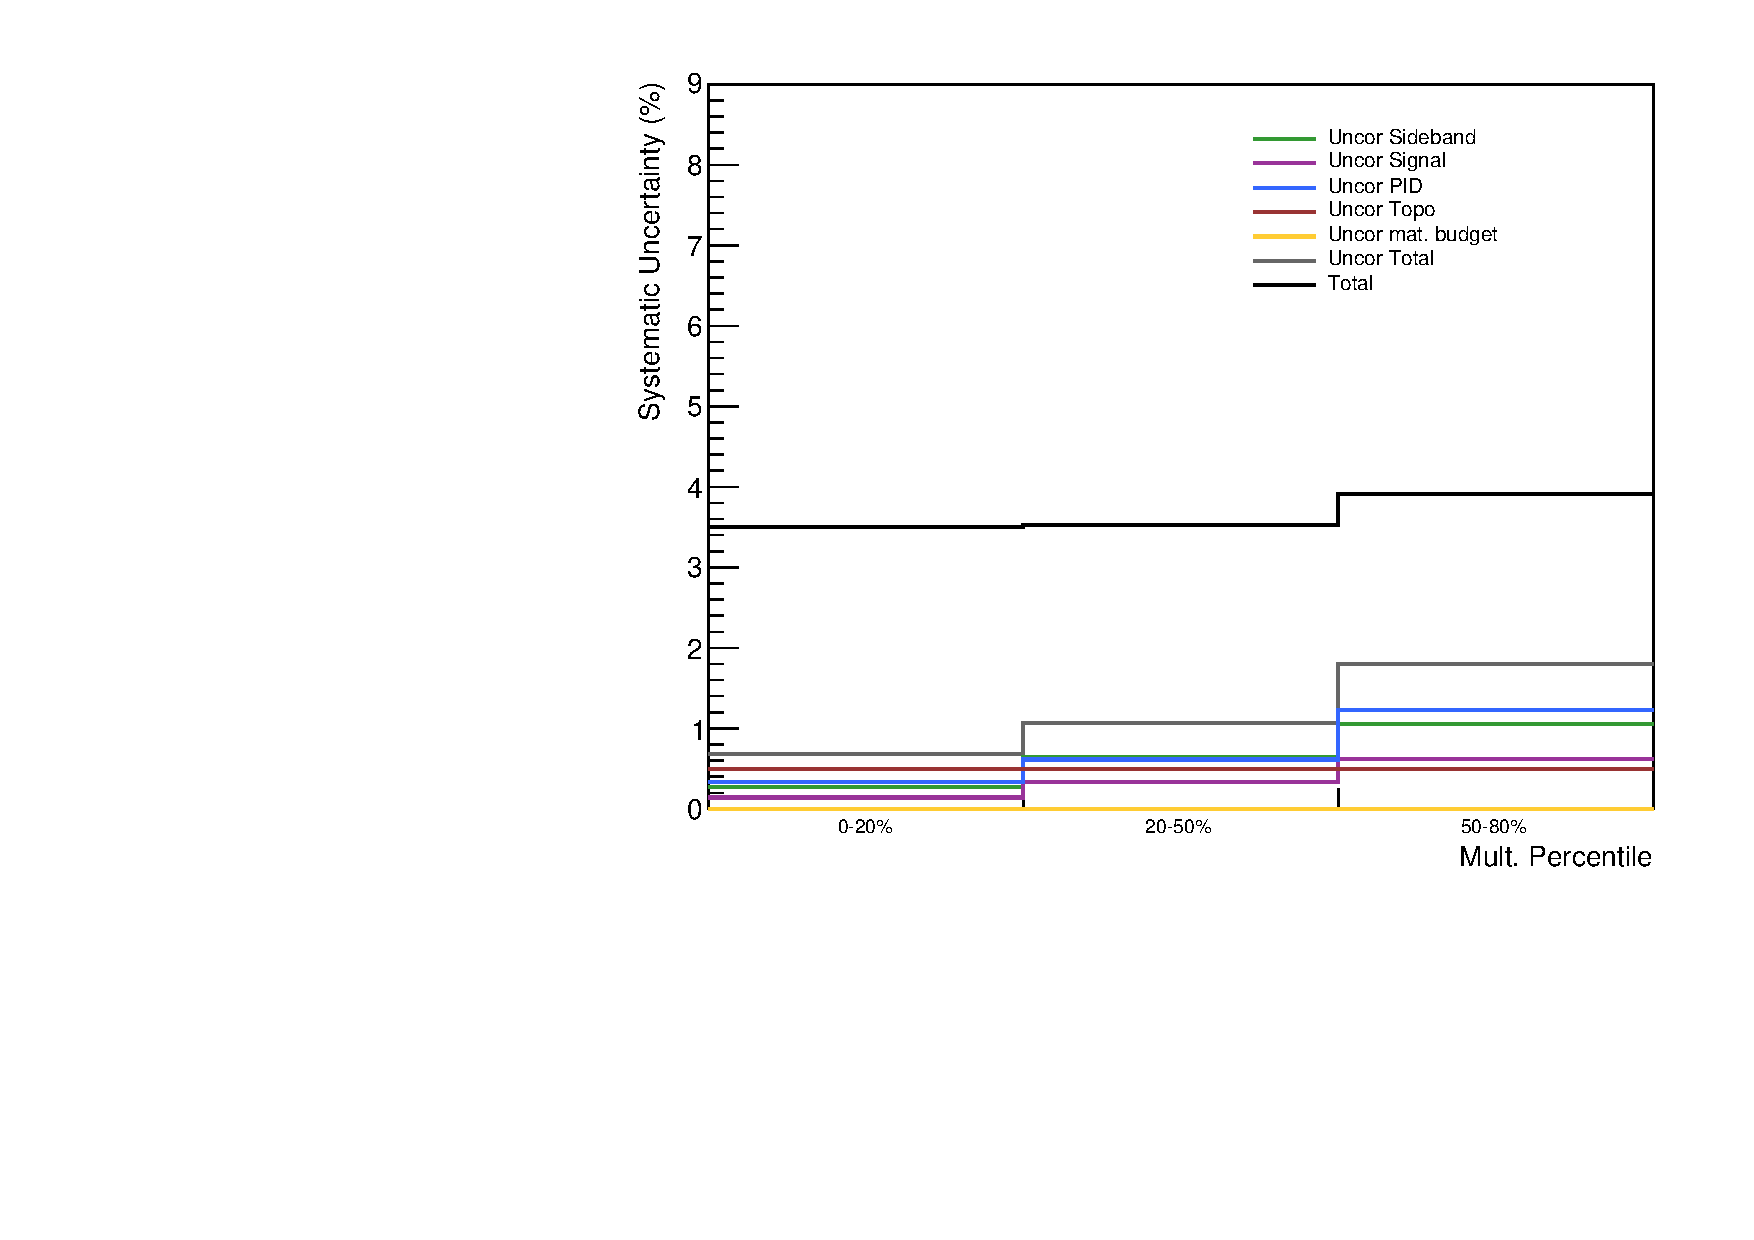
\includegraphics[width=0.48\textwidth]{figures/analysis/nch_dep_systematics_dphi_postbarlow_lowpt.pdf}
    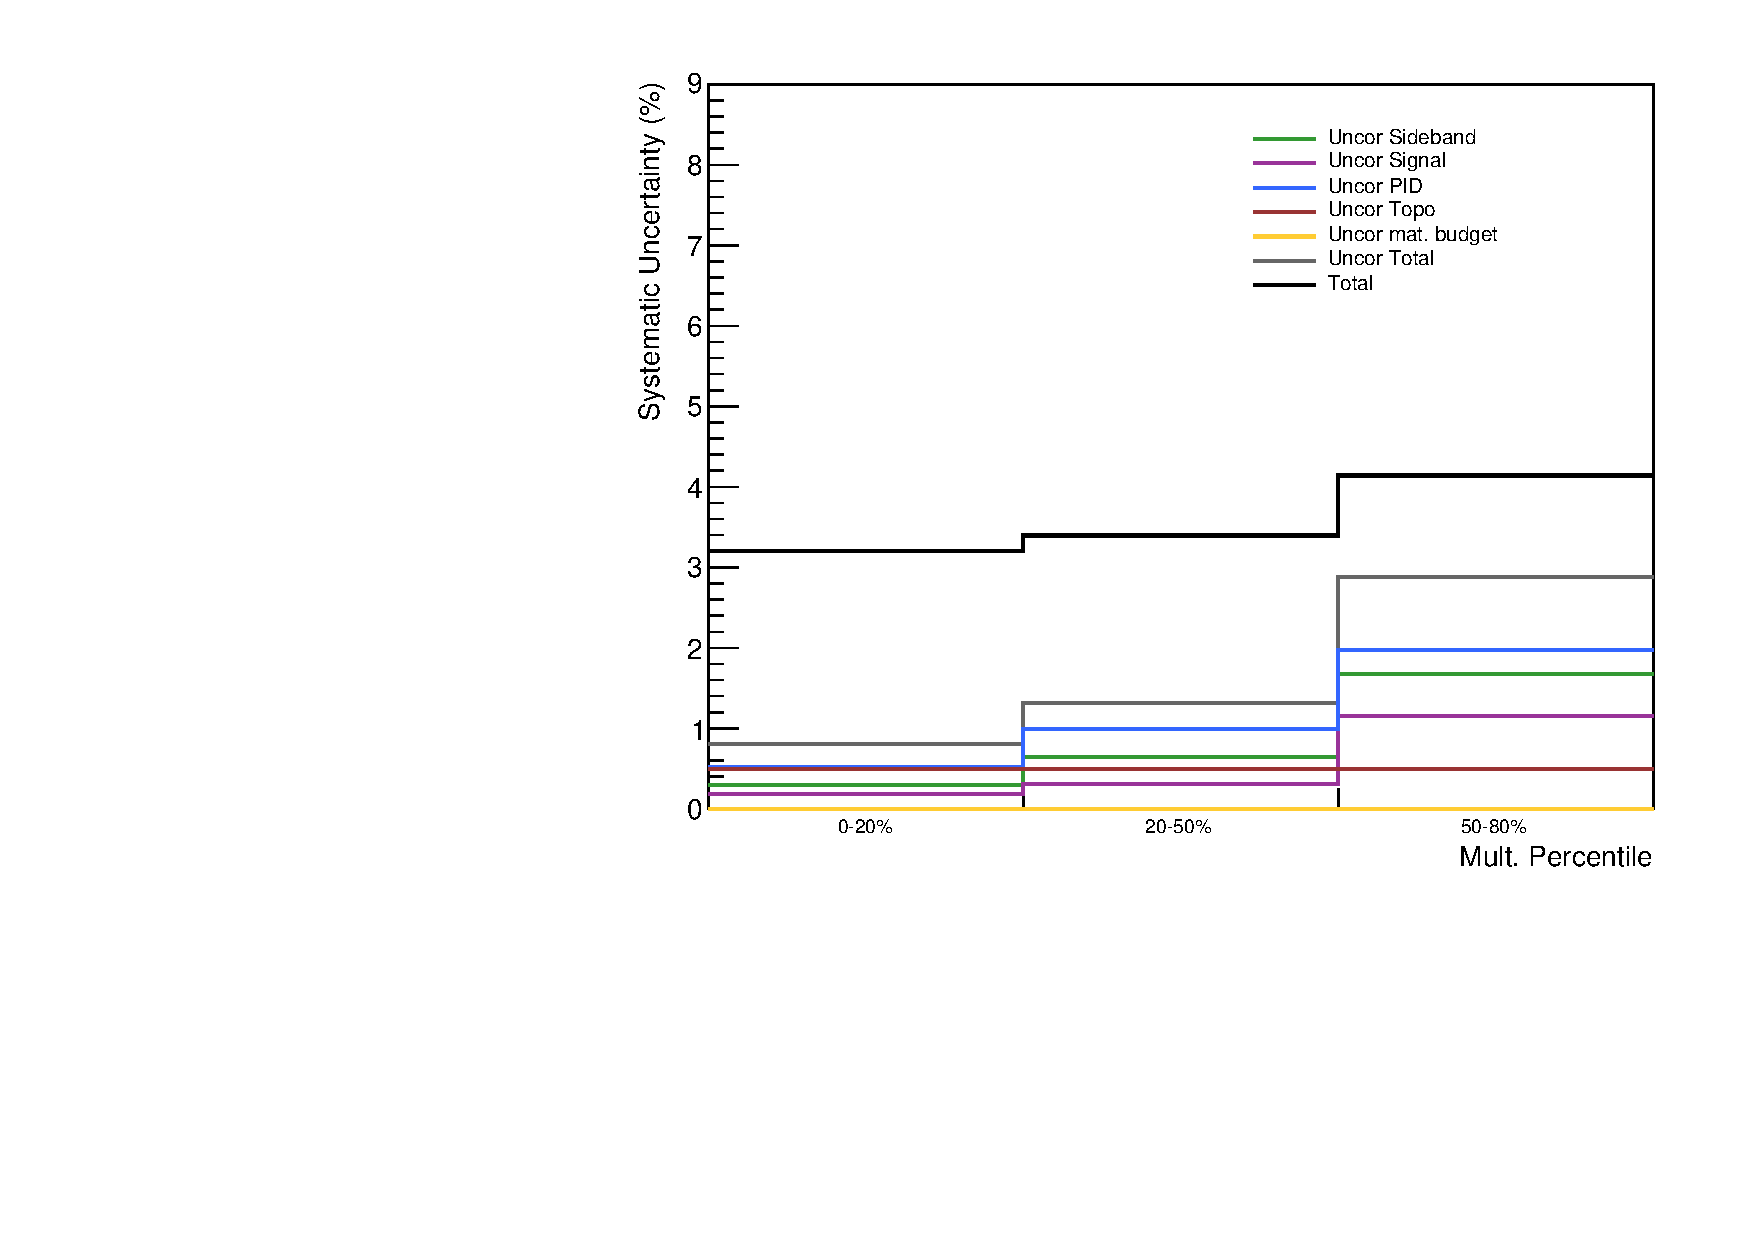
\includegraphics[width=0.48\textwidth]{figures/analysis/nch_dep_systematics_dphi_postbarlow_highpt.pdf}
    \caption{Visual depiction of the multiplicity-uncorrelated systematic errors for the h-$\Lambda$ $\Delta\varphi$ distributions for each multiplicity bin in the low (left) and hig (right) associated \pt bins, along with the total systematic error shown in black.}
    \label{fig:dphi_nch_dep_systematics_plots}
\end{figure}

% \clearpage

\subsection{Yield extraction}
\label{sec:systematics_yield_extraction}

One of the largest sources of systematic uncertainty of this analysis corresponds to the different techniques that can be used to extract the yields in the near-side jet, away-side jet and underlying event from the $\Delta\varphi$ distributions. As mentioned in Section~\ref{sec:yield_extraction}, the equations for extracting these yields are
%
\begin{eqnarray}
    Y_{near} = \int_{-\pi/2}^{\pi/2} (\frac{dN}{d\Delta\varphi}- U(\Delta\varphi))d\Delta\varphi,  \  \ Y_{away} = & \int_{\pi/2}^{3\pi/2} (\frac{dN}{d\Delta\varphi}- U(\Delta\varphi))d\Delta\varphi 
    \label{eq:jet_yields}
    \\ 
    Y_{UE} = \int_{-\pi/2}^{3\pi/2} U(\Delta\varphi)d\Delta\varphi,
    \label{eq:ue_yield}
\end{eqnarray}
%
where $\frac{dN}{d\Delta\varphi}$ is the $\Delta\varphi$ distribution and $U(\Delta\varphi)$ is the underlying event fit. As the $\Delta\varphi$ distribution is present in these equations, all of the previous variations concerning the generation of this distribution must be considered. However, these equations also naturally introduce two new categories of systematic uncertainty: those associated with the underlying event fit, and those associated with the integration of the $\Delta\varphi$ distribution. Both of these categories will be discussed in detail in the following sections.


\subsubsection{Underlying event fit techniques}
\label{sec:ue_fit_systematics}

As the underlying event term $U(\Delta\varphi)$ is present in every yield extraction equation above, any changes in the underlying event fitting procedure will affect the final yield measurements. To maintain compatibility with previous analyses (specifically for the dihadron correlations), the nominal underlying event fit is a straight line to the average of the $\Delta\varphi$ distribution in the ranges $[-\frac{\pi}{2}, -\frac{\pi}{4}) \cup [\frac{\pi}{4}, \frac{5\pi}{8}) \cup [\frac{11\pi}{8}, \frac{3\pi}{2})$. These ranges were initially chosen as there is expected to be little-to-no contamination from the jet components in each range. However, to investigate the effect the UE fitting procedure may have on the final yields, the following alternative methods were considered:
%
\begin{enumerate}
    \item Straight line fit in a more restricted range, specifically $[-\frac{\pi}{2}, -\frac{3\pi}{8}) \cup [\frac{3\pi}{8}, \frac{5\pi}{8}) \cup [\frac{11\pi}{8}, \frac{3\pi}{2})$
    \item Straight line fit using the Zero Yield At Minimum (ZYAM) technique, where the underlying event line is set to the minimum of the $\Delta\varphi$ distribution
    \item Sinusoidal fit which includes a non-zero $v_{2}$ contribution
\end{enumerate}
%
The first two techniques are similar enough to the nominal technique that they will not be explicitly shown in this section. Restricting the range of the flat fit region results in deviations from the nominal procedure of around 2\%, whereas the ZYAM technique gives much larger deviations at about 15\%. Ultimately the ZYAM procedure is not included in the final systematics calculation due to a physical incompatibility, whereby the presence of $v_{2}$ in the higher multiplicity $\Delta\varphi$ distributions causes the ZYAM procedure to massively underestimate the underlying event contribution.

Including a non-zero $v_{2}$ contribution is a much more involved procedure and requires new machinery to be developed, so it will be described in detail in the next section.

\subsubsection{Including a non-zero $v_{2}$ contribution}
\label{sec:ue_fit_v2}

All of the ``straight line'' UE fitting techniques are based on the flatness assumption of the non-jet part of the correlation in \dphi. This means that the dijet axis direction does not affect the non-jet particle distribution's overall shape within an event. However, as mentioned in Section~\ref{sec:collective_effects}, previous \PbPb, \pPb and even \pp collision studies have shown that the QGP's collective flow components ($v_{1}$, $v_{2}$, etc.) influence the phase-space distribution of particles within an event. Using Fourier decomposition, the $\Delta\varphi$ distributions on an event-by-event basis can be written as
%
\begin{equation}
    \label{eq:dphi_fourier_decomposition}
    \frac{dN}{d\Delta\varphi} = a_{0} + \sum_{n=1}^{\infty}2a_{n}cos(n\Delta\varphi),
\end{equation}
%
where $a_{n}$ are the Fourier coefficients. Surprisingly, these coefficients have been shown~\cite{Justin108, Justin109, Justin110} to be related to the collective flow coefficients $v_{n}$ via
%
\begin{equation}
    \label{eq:fourier_vn_relation}
    v_{n} = \frac{a_{n}}{a_{0}}.
\end{equation}
%
This means that even without reconstructing the reaction plane within a specified event, the effects of collective flow are present in the $\Delta\varphi$ distributions. This manifests in the correlation distributions as an underlying event which is not flat with respect to $\Delta\varphi$, but rather sinusoidal. While this is in direct conflict to the initial assumption of a flat underlying event, this nominal choice was made to maintain compatibility with previous measurements of dihadron yields using correlation techniques, which also assume a flat UE in \dphi.

As the $v_{2}$ or ``elliptic flow'' coefficient is the most dominant of the collective flow coefficients measured in \pPb collisions~\cite{Justin111} in the \pt ranges for this analysis, it is the only one considered. Furthermore, the $v_{2}$ coefficients are exceedingly difficult to determine, with fully published papers solely dedicated to measuring the $v_{2}$ for different particle species and collision systems. Luckily, these coefficients have been measured by ALICE in \pPb collisions for both charged hadrons and \lmb baryons across a wide range of \pt~\cite{ALICEv2_1, ALICEv2_2}. As the \pt binning in this analysis is much wider, the weighted average 
%
\begin{equation}
    \label{eq:v2_weighted_average}
    v_{2}^{avg} = \frac{\int_{p_{T, min}}^{p_{T, max}}v_{2}(p_{T})\frac{dN}{dp_{T}}dp_{T}}{\int_{p_{T, min}}^{p_{T, max}}\frac{dN}{dp_{T}}dp_{T}},
\end{equation}
%
is used, where $p_{T, min}$ and $p_{T, max}$ are the minimum and maximum values of \pt in the bins from this analysis (namely $1.5 - 2.5$ and $2.5 - 4.0$ \GeVc). The $v_{2}(\pt)$ values for charged hadrons and \lmb baryons are taken from ~\cite{ALICEv2_1}, and $dN/dp_{T}$ is taken from the published \pt spectra for charged hadrons and \lmb baryons from ~\cite{PtSpectra}, plots of which can be seen in Figures~\ref{fig:v2_plot} ($v_{2}$) and \ref{fig:pt_spectra_plot} (\pt spectra). The values of $v_{2}^{avg}$ for each \pt bin are shown in Table~\ref{tab:v2_values}. Note that the trigger $v_{2}$ remains the same, as the trigger \pt range is fixed for this analysis. The $\Lambda$ $v_{2}$ is markedly higher than the charged hadron $v_{2}$, which ultimately manifests itself as a larger deviation from the nominal UE fit when compared to the dihadron case.
%
\begin{table}[t]
    \centering
    \caption{$v_{2}$ values used in this analysis for each associated \pt bin. The values were calculated as the weighted average of published \pt-differential $v_{2}$ measurements with the published \pt spectra, taken across the entire associated \pt range.}
    \label{tab:v2_values}
    \begin{tabular}{ l c c c c }
    \hline
    $p_{T}^{\text{assoc.}}$ & $v_{2}^{\text{trig.}}$ & $v_{2}^{\text{assoc. h}}$ & $v_{2}^{\text{assoc.} \Lambda}$ \\
    \hline
    1.5 - 2.5 & 0.092 & 0.100 & 0.075 \\
    2.5 - 4.0 & 0.092 & 0.119 & 0.137 \\
    \hline
    \end{tabular}
\end{table}
%
Unfortunately there are few multiplicity-dependent measurements of the $v_{2}$ coefficients for identified particle species. Because of this, the $v_{2}$ values from Table~\ref{tab:v2_values} are used only in the 0-20\% multiplicity bin, with the $v_{2}$ values for the 20-50\% and 50-80\% multiplicity bins taken as 0.85 and 0.50 times the 0-20\% value, respectively.

\begin{figure}[ht]
    \centering
    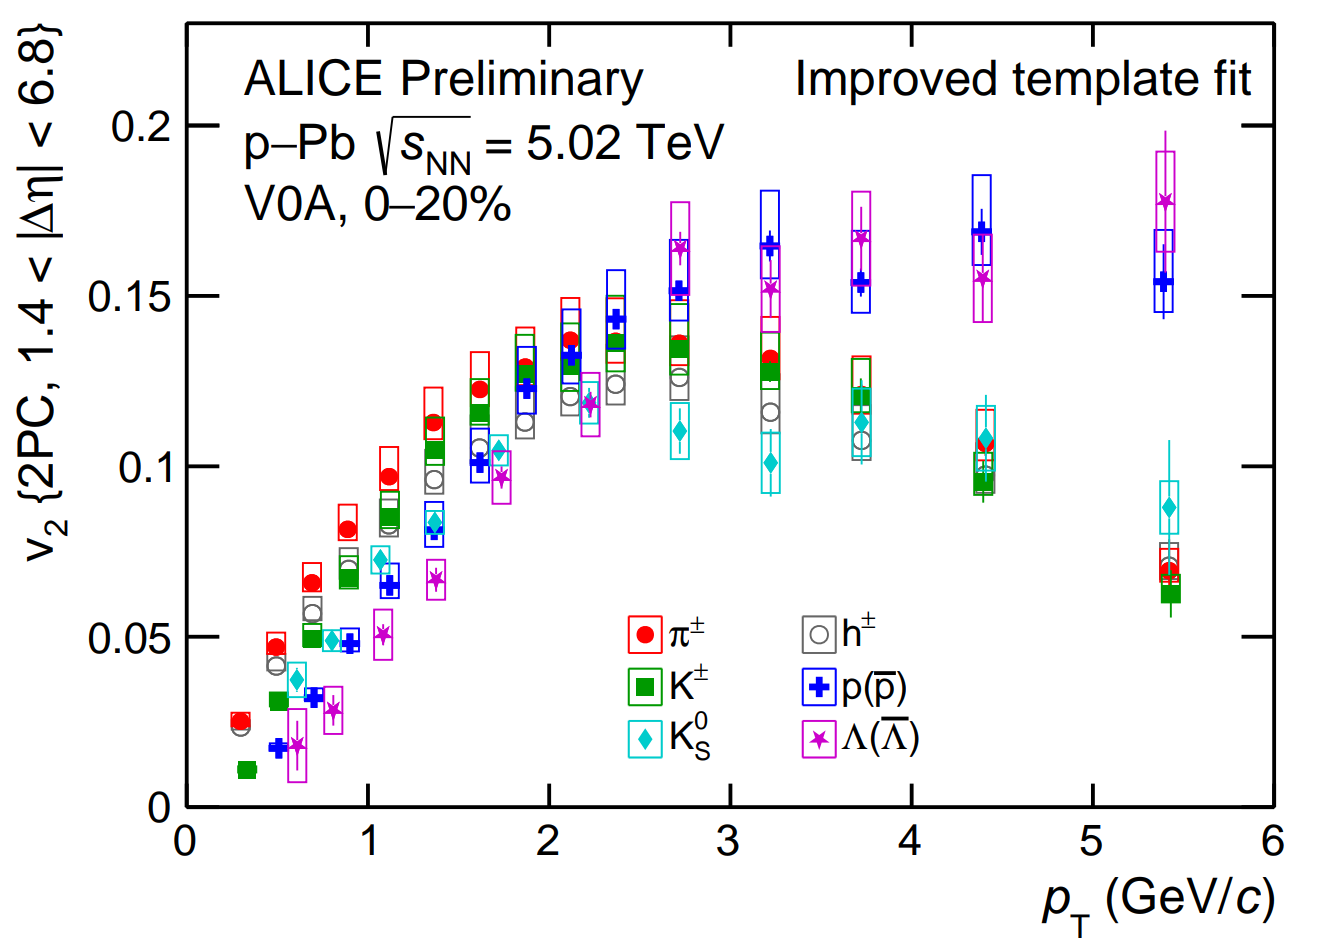
\includegraphics[width=0.8\textwidth]{figures/analysis/v2_diagram.png}
    \caption{The $v_{2}$ values for identified hadrons as a function of \pt, taken from~\cite{ALICEv2_1}.}
    \label{fig:v2_plot}
\end{figure}

\begin{figure}[ht]
    \centering
    \begin{minipage}{0.48\textwidth}
        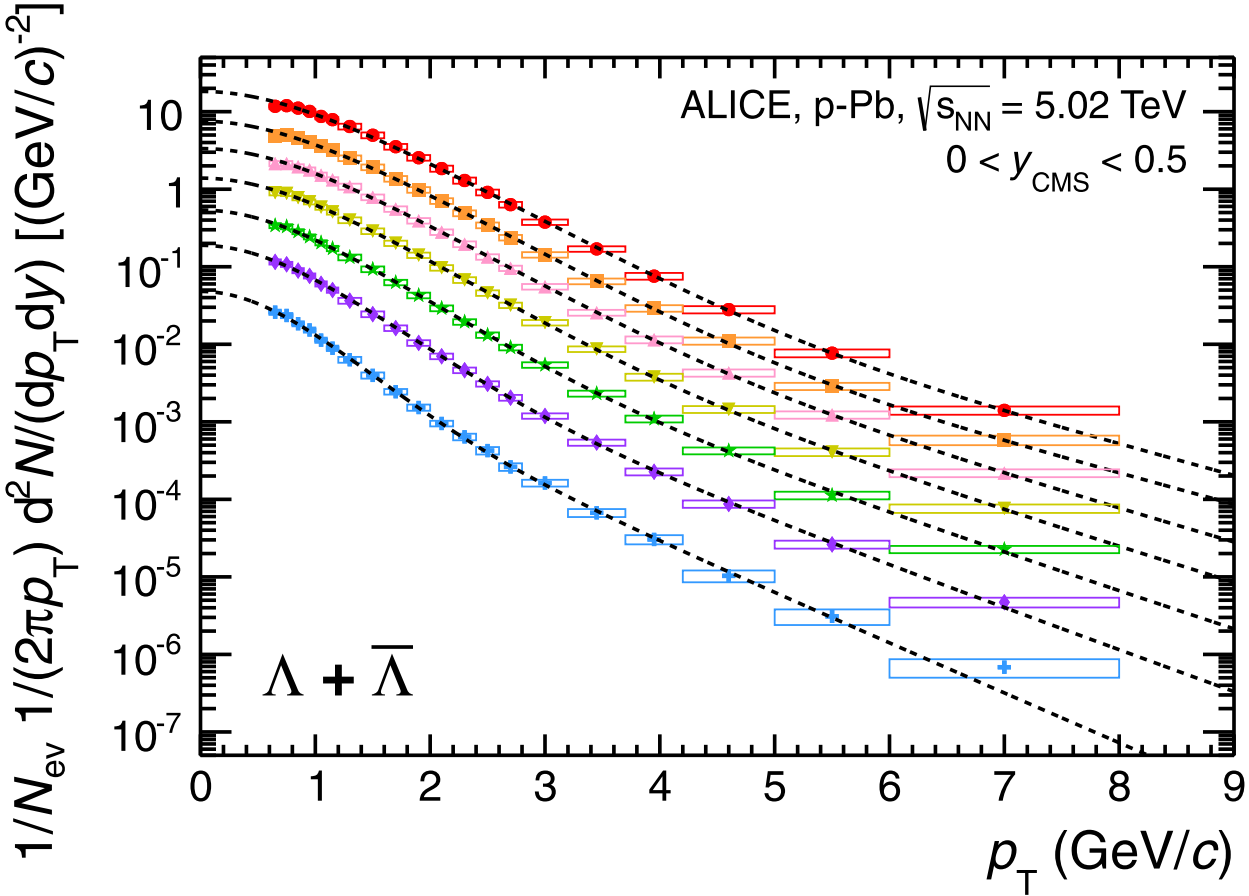
\includegraphics[width=\textwidth]{figures/analysis/lambda_pt_spectra.png}
        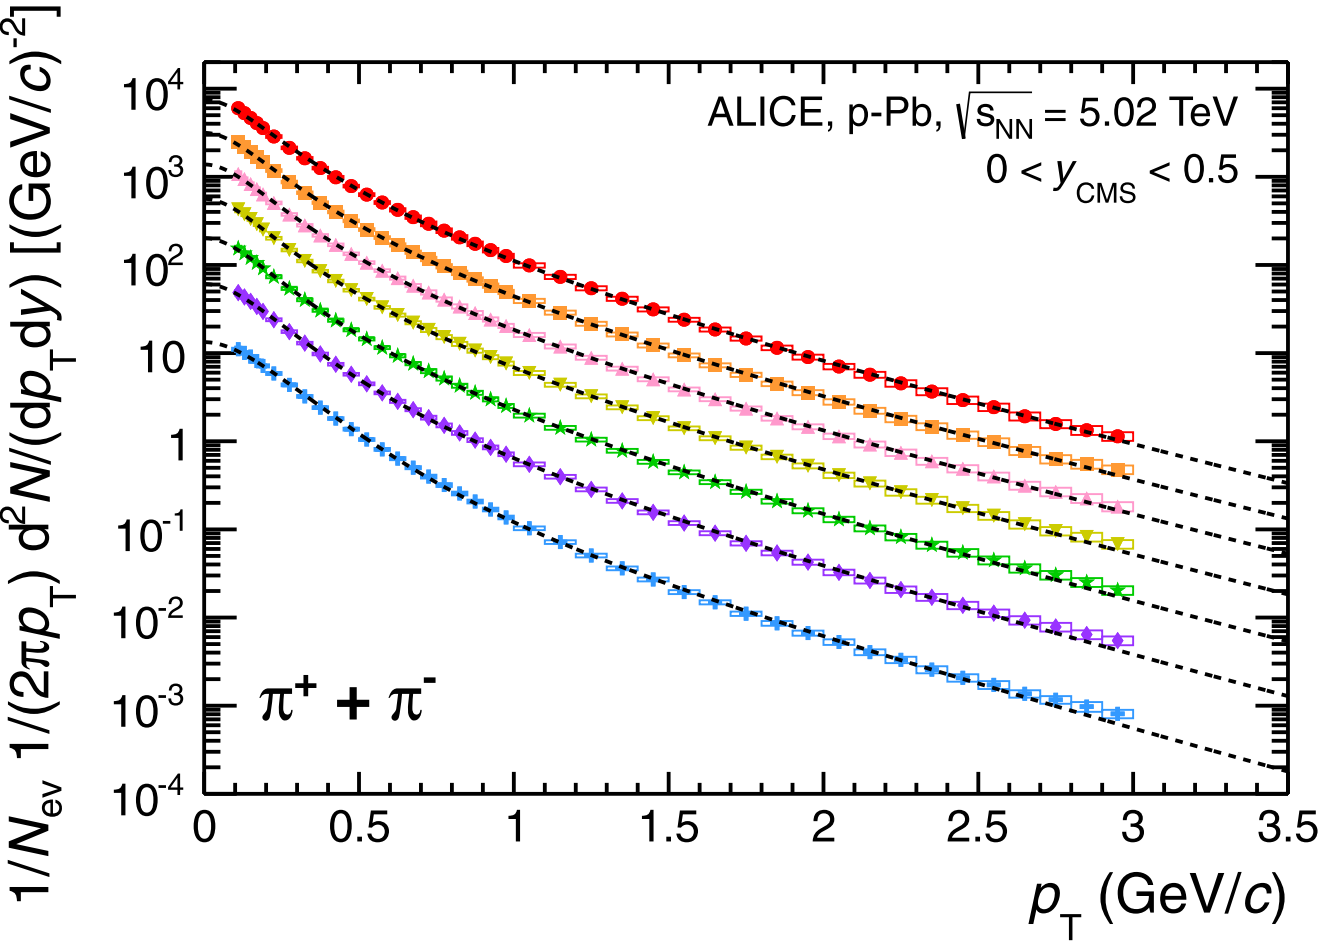
\includegraphics[width=\textwidth]{figures/analysis/pion_pt_spectra.png}
    \end{minipage}
    \hspace{1.2cm}
    \begin{minipage}{0.40\textwidth}
        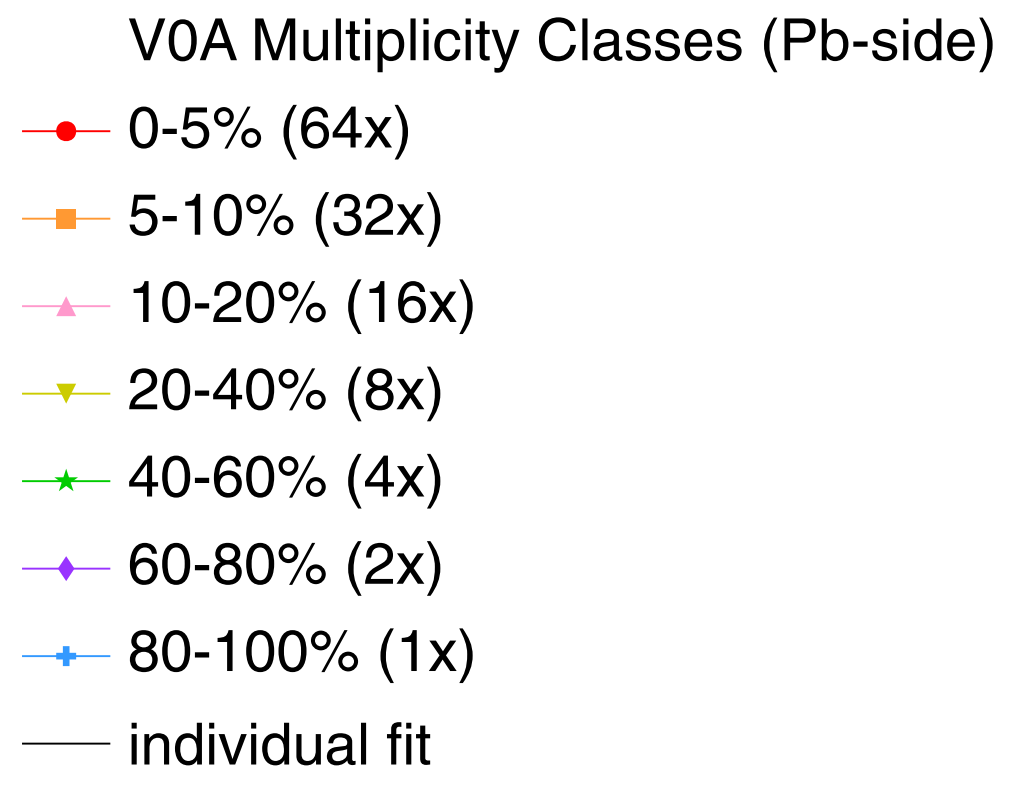
\includegraphics[width=0.8\textwidth]{figures/analysis/pt_spectra_legend.png}
    \end{minipage}
    \caption{The published~\cite{ALICEMatBud} \pt spectra for \lmb baryons (top) and charged hadrons ($\approx$ pions) (bottom), used to compute the weighted average of the $v_{2}$ coefficients across the wide momentum bins used in this analysis.}
    \label{fig:pt_spectra_plot}
\end{figure}

Using these $v_{2}$ values, the underlying event is estimated by fitting the function 
%
\begin{equation}
    \label{eq:ue_v2}
    U_{v_{2}}(\Delta\varphi) = A\times(1 + 2v_{2}^{\text{trig.}}v_{2}^{\text{assoc.}}cos(2\Delta\varphi))
\end{equation}
%
in the ranges $-\pi/2 < \Delta\varphi < -1$ and $1 < \Delta\varphi < +\pi/2$, where little jet contribution is expected. The underlying event \textbf{pedestal} $A$ is allowed to vary during the fit, but the $v_{2}$ values are fixed. Examples of h-\lmb and h-h $\Delta\varphi$ distributions with the UE fit using this procedure are shown in Figure~\ref{fig:v2_fit_examples}.

\begin{figure}[ht]
    \centering
    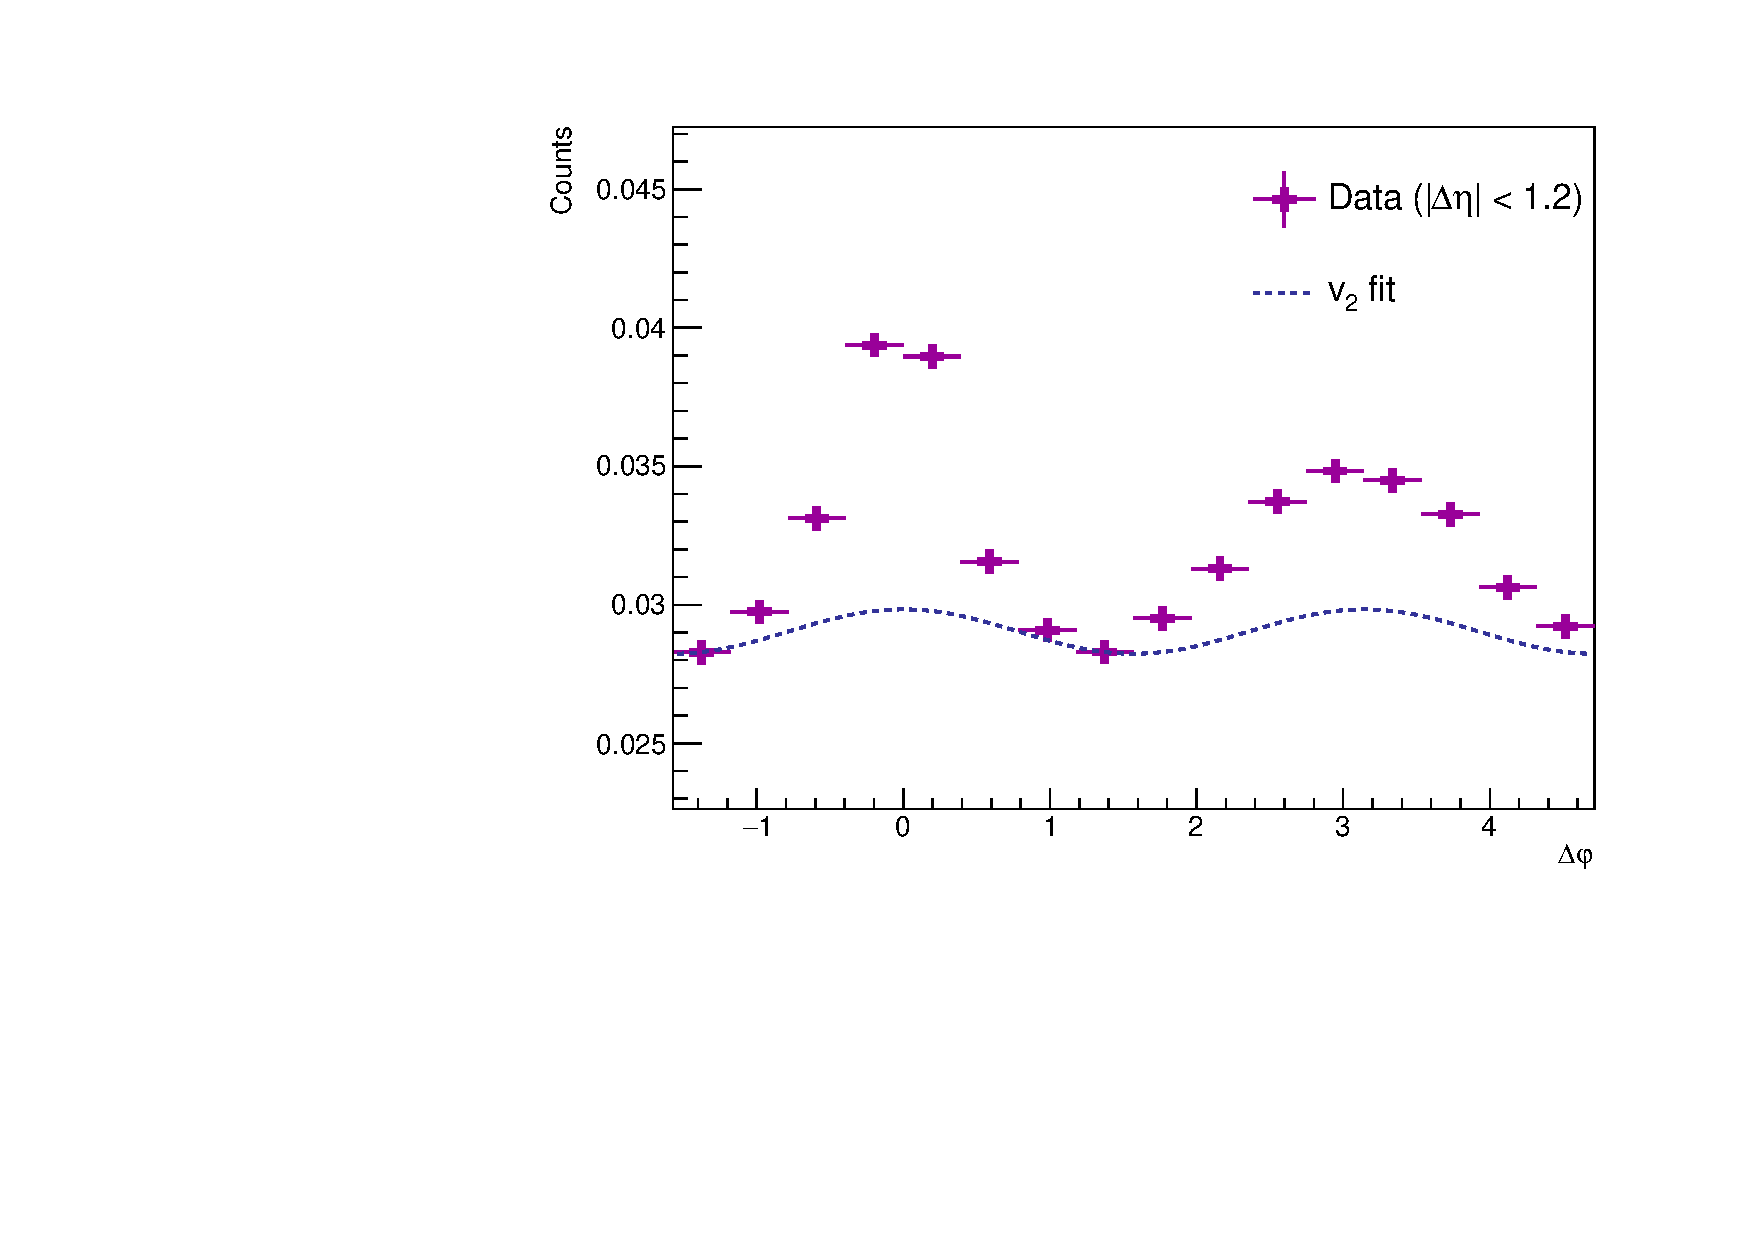
\includegraphics[width=0.49\textwidth]{figures/analysis/v2fit_h_lambda_cent_0_20_trigger_4_8_assoc_25_4.pdf}
    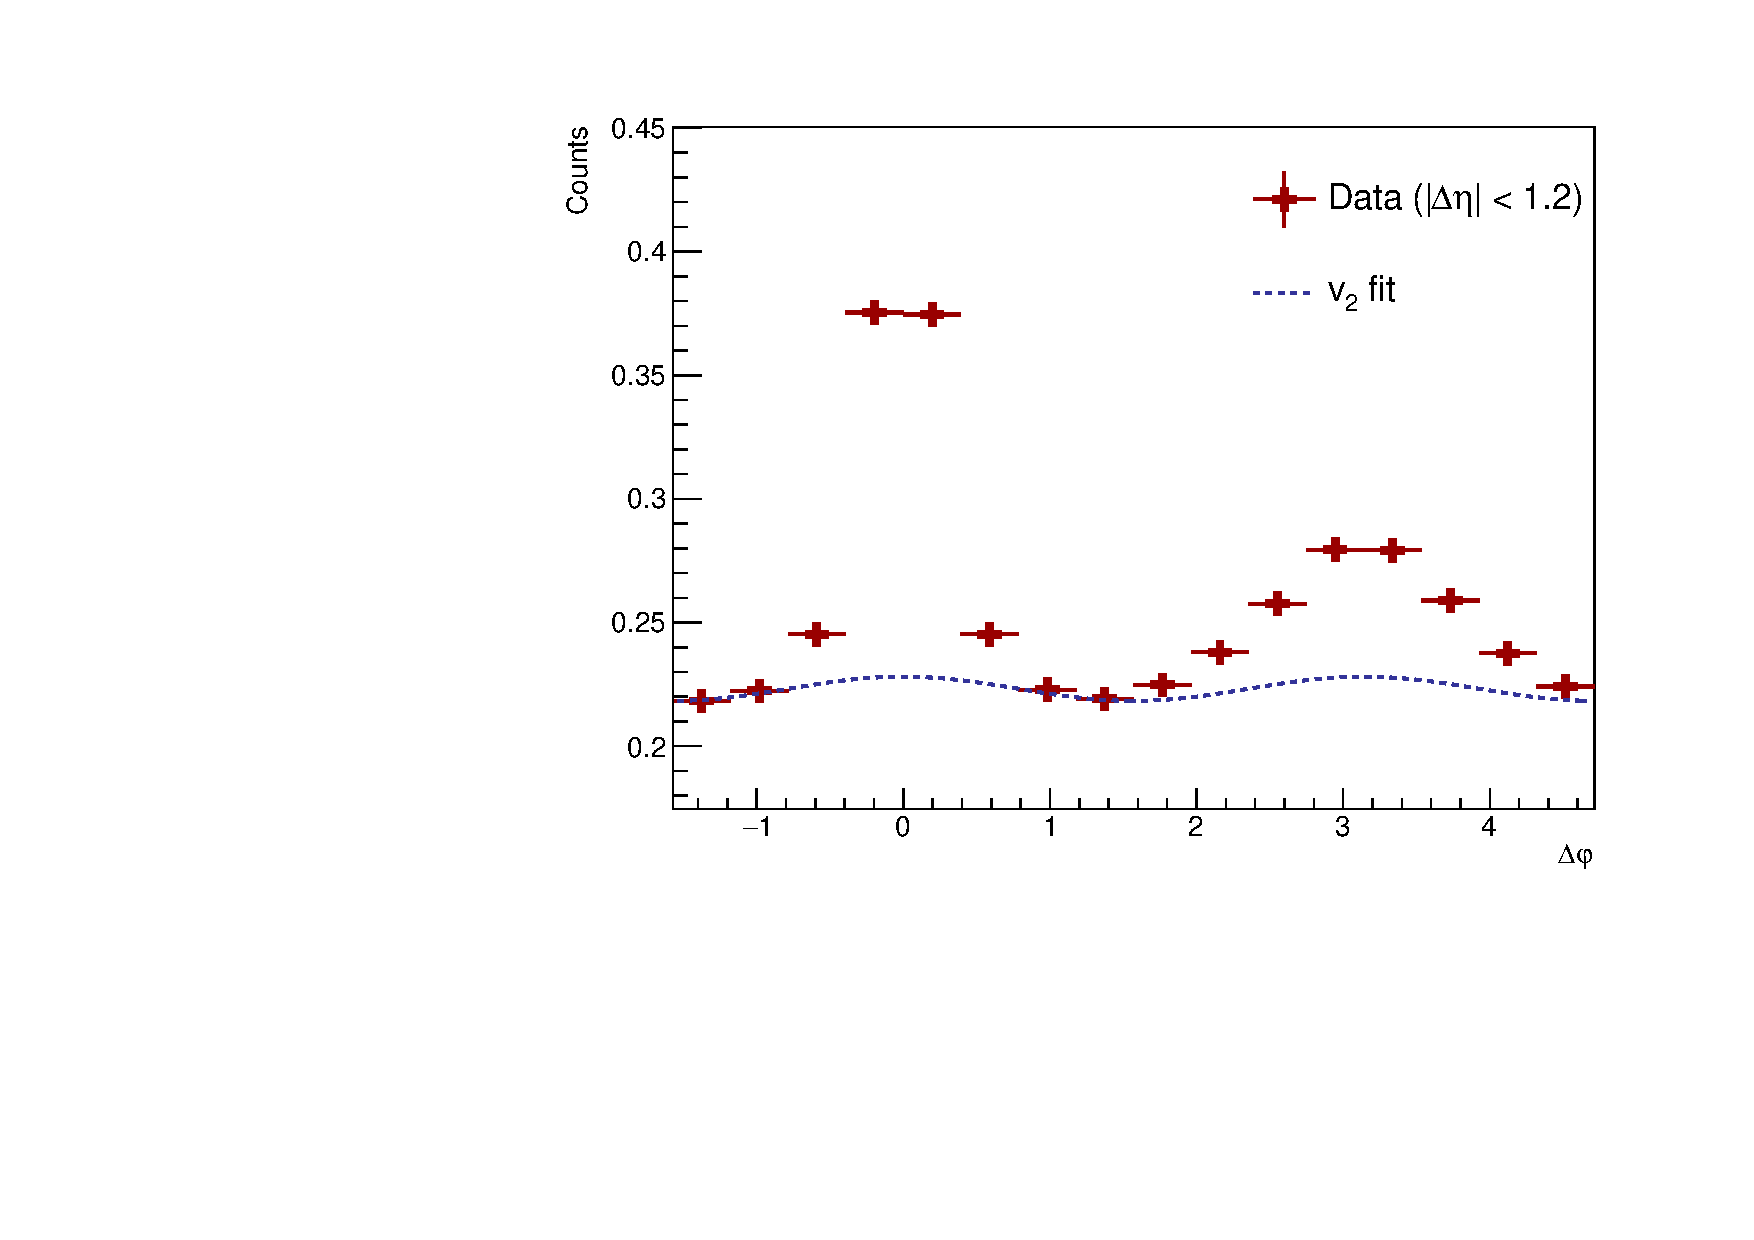
\includegraphics[width=0.49\textwidth]{figures/analysis/v2fit_h_h_cent_0_20_trigger_4_8_assoc_25_4.pdf}
    \caption{Examples of the underlying event fit using the $v_{2}$-based procedure for the h-\lmb (left) and h-h (right) $\Delta\varphi$ distributions in the 0-20\% multiplicity bin in the higher associated \pt bin.}
    \label{fig:v2_fit_examples}
\end{figure}

The validty of this procedure can be tested by examining the $\Delta\varphi$ distributions at large $\Delta\eta$, where the near-side jet component is minimal, leaving just the UE at small $\Delta\varphi$\footnote{At large $\Delta\varphi$, the away-side ridge is still present.}. In fact, this procedure is often used to determine the $v_{2}$ coefficients in the first place. In this case, however, it will just be used to serve as a sanity check for both the fitting procedure and the fixed $v_{2}$ coefficients from~\ref{tab:v2_values}. If the UE fit matches the near-side of the $\Delta\varphi$ distribution at large $\Delta\eta$, then the $v_{2}$ coefficients and fitting procedure are likely valid. Examples of the $\Delta\varphi$ distributions with $|\Delta\eta| > 1.4$ and $|\Delta\eta| < 1.2$ showing the $v_{2}$-based UE fit can be seen in Figure~\ref{fig:v2_fit_large_deta}. These are generated in the highest multiplicity and momentum bins, where the effects of the $v_{2}$ contribution are maximal. Both the h-\lmb and h-h $\Delta\varphi$ distributions show good agreement between the UE fit and the data at small $\Delta\varphi$ and large $\Delta\eta$, where the near-side jet peak and away-side ridge are no longer present, pointing to the validity of the $v_{2}$-based UE fitting procedure.

\begin{figure}[ht]
    \centering
    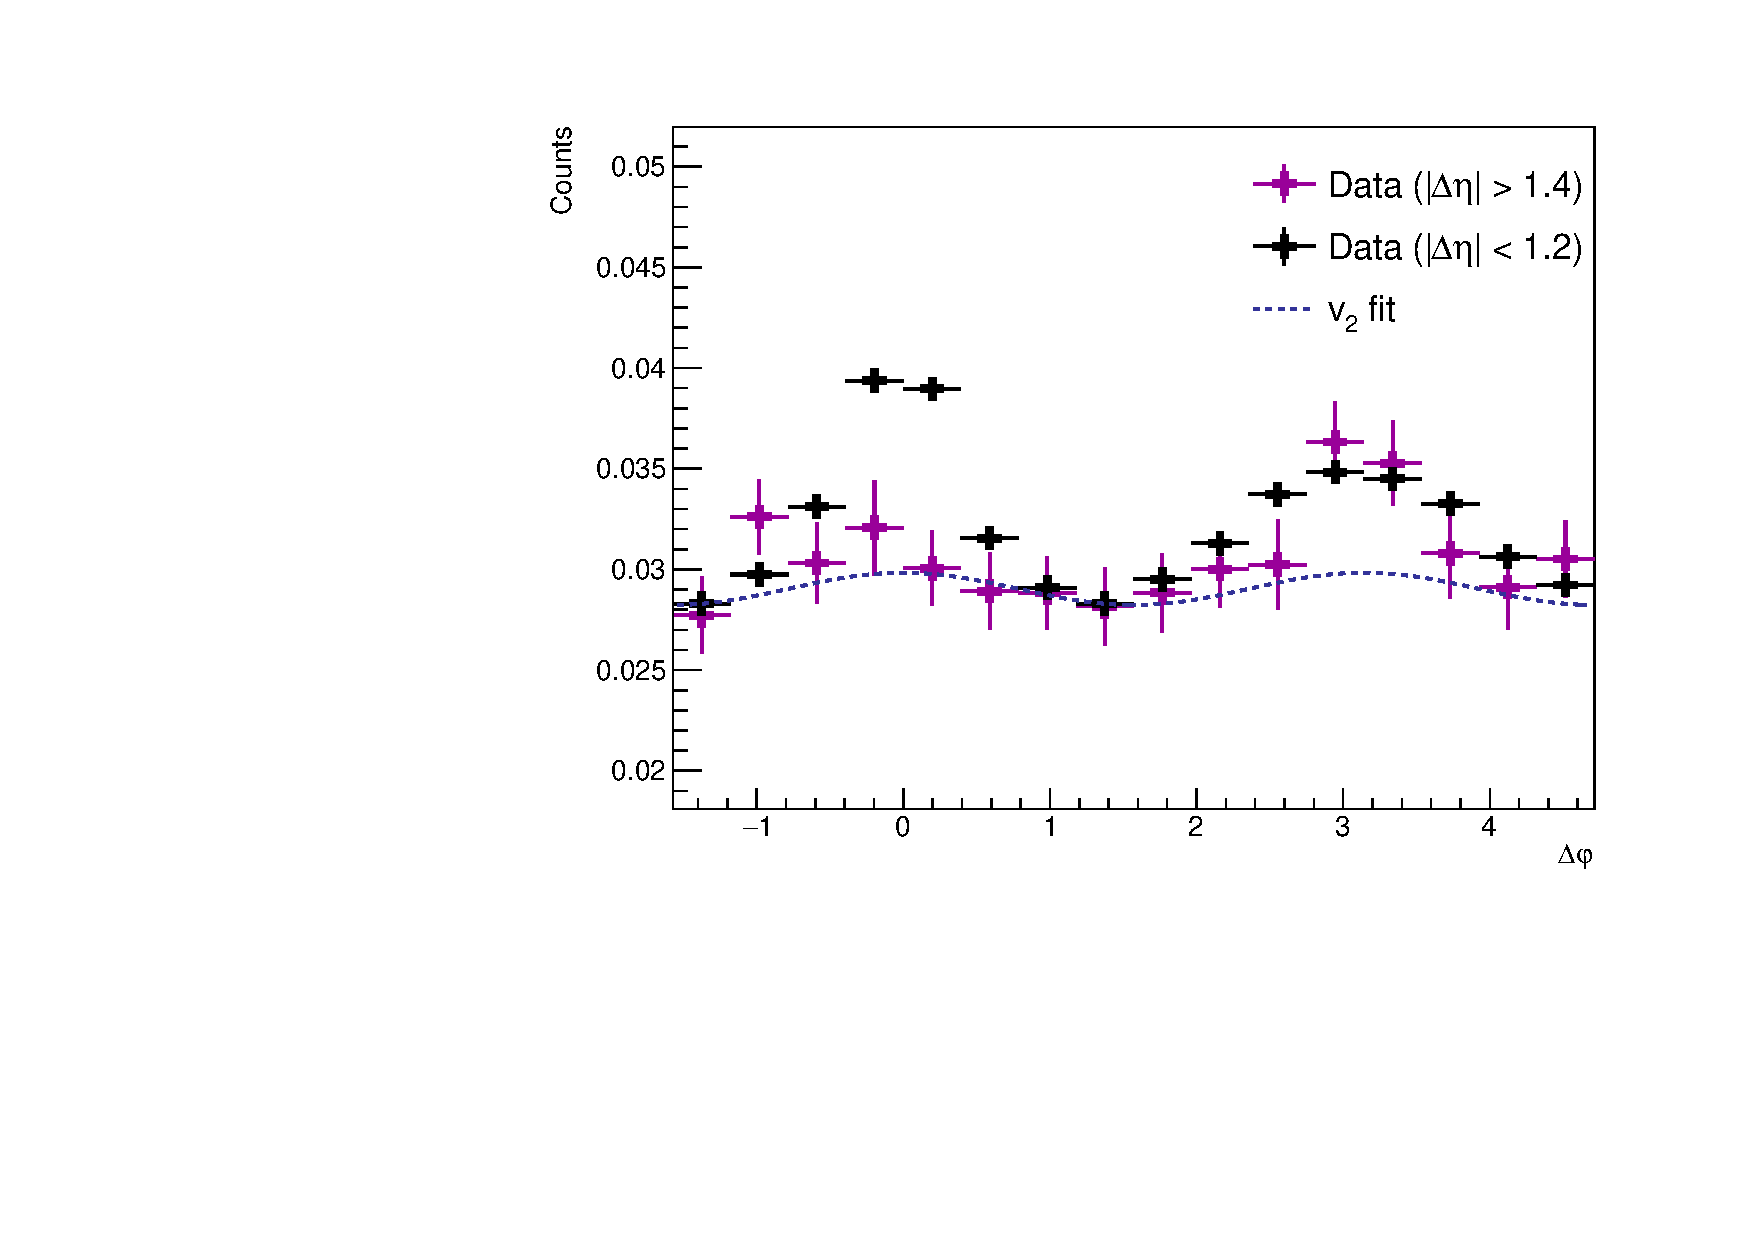
\includegraphics[width=0.49\textwidth]{figures/analysis/v2fit_largedeta_h_lambda_cent_0_20_trigger_4_8_assoc_25_4.pdf}
    \includegraphics[width=0.49\textwidth]{figures/analysis/v2fit_largedeta_h_h_cent_0_20_trigger_4_8_assoc_25_4.pdf}
    \caption{The h-\lmb (left) and h-h (right) $\Delta\varphi$ distributions in the 0-20\% multiplicity bin and higher \pt bin at small and large values of $\Delta\eta$, with the UE fit using the $v_{2}$-based procedure shown in blue. The fits are in good agreement with data in both cases.}
    \label{fig:v2_fit_large_deta}
\end{figure}

The effects of including $v_{2}$ has on the extracted h-\lmb and h-h yields in each region is not at all obvious at first glance. For the most central collisions, the inclusion of $v_{2}$ results in nearly a 5\% decrease for the jet-like yields when compared to the nominal technique. This can mostly be seen in Figure~\ref{fig:v2_fit_examples}, where the peaks of the sinusoidal fit achieve their maxima within the near- and away-side components of the jet, causing the overall yields to be lower than those obtained by the flat UE assumption. However, at lower multiplicities (20-50\%, 50-80\%), the extracted h-\lmb and h-h jet-like yields actually exhibit a slight increase of around 5\% in their extracted yields when compared to those measured using the nominal UE fit. This is due to the variation of the pedestal $A$ in Equation~\ref{eq:ue_v2} during the fit, which results in a smaller pedestal value than the nominal fit in these multiplicity ranges. The extracted underlying event yield never deviates by more than 3\% from the yield obtained using the nominal procedure for all multiplicity and momentum bins for both the h-\lmb and h-h cases.

\subsubsection{Integration procedures}
\label{sec:integration_procedures}

The general yield-extraction equation
%
\begin{equation}
    \label{eq:general_yield}
    Y_{\Delta\varphi} = \int_{\Delta\varphi_1}^{\Delta\varphi_2} (\frac{dN}{d\Delta\varphi}- U(\Delta\varphi))d\Delta\varphi
\end{equation}
%
leaves some room for interpretation. Obviously the $\Delta\varphi$ distributions shown thus far are in some way related to $dN/d\Delta\varphi$, but integrals prefer continuous integrands, which the $\Delta\varphi$ distributions are clearly not as they have finitely many (16) bins. Furthermore, there is nothing explicity preventing 
%
\begin{equation}
    \frac{dN}{d\Delta\varphi} < U(\Delta\varphi),
\end{equation}
%
possibly resulting in a \textit{negative} yield, which is clearly unphysical. There are a few ways to alleviate these issues, which are discussed in this section.

For all of the yield extraction procedures discussed thus far, the usage of the integration symbol in Equation~\ref{eq:general_yield} is \textit{slightly} misleading: the yields are actually calculated by summing the bin contents of the $\Delta\varphi$ distribution in the specified range, and subtracting off the value of $U(\Delta\varphi)$ at the center of each bin. To be more explicit, the yields are calculated as
%
\begin{equation}
    \label{eq:yield_sum}
    Y_{\Delta\varphi} = \sum_{i=L}^{U} (\frac{dN}{d\Delta\varphi_{i}}- U(\Delta\varphi_{i})),
\end{equation}
%
where $L$ and $U$ are the bin numbers of the Lower and Upper $\Delta\varphi$ bins in the specified range, $dN/d\Delta\varphi_{i}$ is the value of the correlation distribution in the ith \dphi bin, and $U(\Delta\varphi)$ is the value of $U$ in the center of the ith \dphi bin. 

Equation~\ref{eq:yield_sum} provides an easy way to deal with the negative yield issue: if the value of $U(\Delta\varphi_{i})$ is greater than the value of $dN/d\Delta\varphi_{i}$ in a given bin, the yield in that bin is set to zero. While this is not done for the nominal yield extraction procedure in this analysis, it is a completely reasonable technique and is therefore explored in the systematic uncertainty analysis. Using the flat UE assumption with the UE average taken in the nominal range, the results are relatively unsurprising: the yields extracted using this procedure are strictly higher than those extracted using the main procedure where negative contributions are allowed. However, the deviations never exceed more than 3.5\%, with the average deviation being around 2\% for both the h-\lmb and h-h cases.

Another way to address the lack of continuity in the $\Delta\varphi$ distributions is to fit these distributions with continuous functions, then use the corresponding fit for the integration in Equation~\ref{eq:general_yield}. This thesis considers two such functions, which are presented in the following two sections.

\subsubsection{The double Gaussian fit}
\label{sec:double_gaus_fit}

There are a number of functions that may appear suitable to fit the $\Delta\varphi$ distributions, but given the Gaussian-like appearance of the near- and away-side jet components, a double Gaussian fit is a natural choice. The double Gaussian fit function is given by
%
\begin{equation}
    \label{eq:double_gaus}
    \begin{split}
	&f(\Delta\varphi)  = U + A_{\text{NS}} e^{\frac{(\Delta\varphi - \mu_{\text{NS}})^2}{2\sigma_{\text{NS}}}} + A_{\text{AS}} e^{\frac{(\Delta\varphi - \mu_{\text{AS}})^2}{2\sigma_{\text{AS}}}} \\
    & + A_{\text{NS}}^{\text{mirror}} e^{\frac{(\Delta\varphi - \mu_{\text{NS}} + 2\pi)^2}{2\sigma_{\text{NS}}}} + A_{\text{AS}}^{\text{mirror}} e^{\frac{(\Delta\varphi - \mu_{\text{AS}} - 2\pi)^2}{2\sigma_{\text{AS}}}},
    \end{split}
\end{equation}
%
where $A$ and $\mu$ are the amplitude and means of the Gaussian components, and the subscript ``NS'' (``AS'') refers to the near-side (away-side) jet component. The ``mirror'' terms are added to account for the $2\pi$ periodicity of the $\Delta\varphi$ distribution, and are required to obtain a convergent fit. The $U$ term describes a flat underlying event, and is fixed to the average of the $\Delta\varphi$ distribution in the regions $[-\frac{\pi}{2}, -\frac{\pi}{4}) \cup [\frac{\pi}{4}, \frac{5\pi}{8}) \cup [\frac{11\pi}{8}, \frac{3\pi}{2})$, as is done for the nominal UE determination procedure. Furthermore, the mean in the near-side gaussian (and corresponding mirror term) is fixed to 0 ($2\pi$) and the mean in the away-side guassian (and corresponding mirror term) is fixed to $\pi$ ($-\pi$), leaving only the amplitudes and widths to vary freely. The double Gaussian fits to both the h-\lmb and h-h correlation distributions for every multiplicity and momentum bin are shown in Figures~\ref{fig:double_gaus_fits_lambda} (h-\lmb) and~\ref{fig:double_gaus_fits_h}. The fits generally describe the data quite well, though an extreme amount of effort went in to ensuring the convergence of each fit due to an inordinate amount of instability. 

The yields extracted using the double Gaussian fit are nearly identical to those extracted using the nominal bin-wise integration procedure, with deviations from the nominal procedure never exceeding 1\% for either the h-\lmb or h-h cases. This indicates two things:
%
\begin{enumerate}
    \item The fits describe the data quite well, and
    \item The differences between Equations~\ref{eq:general_yield} and~\ref{eq:yield_sum} are mostly aesthetic, so long as (1) holds and the choice of $U(\Delta\varphi)$ is consistent.
\end{enumerate}
%
As the deviations are so small, this procedure ends up excluded from the final systematic uncertainty calculation after the Barlow check in Section~\ref{sec:barlow_check_yield}, but the fits are still used for the systematic studies involving the near- and away-side jet widths discussed in Section~\ref{sec:systematics_width}.


\begin{figure}[ht]
    \centering
    \includegraphics[width=0.48\textwidth]{figures/analysis/h_lambda_dphi_gaus_0_20_lowpt.pdf}
    \includegraphics[width=0.48\textwidth]{figures/analysis/h_lambda_dphi_gaus_0_20_highpt.pdf}
    \includegraphics[width=0.48\textwidth]{figures/analysis/h_lambda_dphi_gaus_20_50_lowpt.pdf}
    \includegraphics[width=0.48\textwidth]{figures/analysis/h_lambda_dphi_gaus_20_50_highpt.pdf}
    \includegraphics[width=0.48\textwidth]{figures/analysis/h_lambda_dphi_gaus_50_80_lowpt.pdf}
    \includegraphics[width=0.48\textwidth]{figures/analysis/h_lambda_dphi_gaus_50_80_highpt.pdf}
    \caption{The final per-trigger h-\lmb $\Delta\varphi$ correlation distributions with the full double Gaussian fit for the 0-20\% (top), 20-50\%(middle) and 50-80\% (bottom) multiplicity bins in the lower (left) and higher (right) associated \pt bins. The UE fit is also shown as a dashed line.}
    \label{fig:double_gaus_fits_lambda}
\end{figure}
\begin{figure}[ht]
    \centering
    \includegraphics[width=0.48\textwidth]{figures/analysis/h_h_dphi_gaus_0_20_lowpt.pdf}
    \includegraphics[width=0.48\textwidth]{figures/analysis/h_h_dphi_gaus_0_20_highpt.pdf}
    \includegraphics[width=0.48\textwidth]{figures/analysis/h_h_dphi_gaus_20_50_lowpt.pdf}
    \includegraphics[width=0.48\textwidth]{figures/analysis/h_h_dphi_gaus_20_50_highpt.pdf}
    \includegraphics[width=0.48\textwidth]{figures/analysis/h_h_dphi_gaus_50_80_lowpt.pdf}
    \includegraphics[width=0.48\textwidth]{figures/analysis/h_h_dphi_gaus_50_80_highpt.pdf}
    \caption{The final per-trigger h-h $\Delta\varphi$ correlation distributions with the full double Gaussian fit for the 0-20\% (top), 20-50\%(middle) and 50-80\% (bottom) multiplicity bins in the lower (left) and higher (right) associated \pt bins. The UE fit is also shown as a dashed line.}
    \label{fig:double_gaus_fits_h}
\end{figure}

\clearpage

\subsubsection{The von Mises fit}
\label{sec:von_mises_fit}

While only briefly mentioned in Section~\ref{sec:width_extraction} in the context of extracting the near- and away-side jet widths, the von Mises distribution is another natural choice for fitting the $\Delta\varphi$ distributions due to its combined Gaussian-like behaviour while naturally exhibiting $2\pi$-periodicity (which was ``forced'' onto the double Gaussian fit via the mirror terms). As a reminder, the von Mises fit function is given by
%
\begin{equation}
    \label{eq:von_mises}
    f(\Delta\varphi) = U(\Delta\varphi) + \frac{A_{\text{NS}}}{2\pi I_0(k_{\text{NS}})} e^{k_{\text{NS}}cos(\Delta\varphi - \mu_{\text{NS}})} + \frac{A_{\text{AS}}}{2\pi I_0(k_{\text{AS}})} e^{k_{\text{AS}}cos(\Delta\varphi - \mu_{\text{AS}})},
\end{equation}
%
where $A$ and $\mu$ are as they were in Equation~\ref{eq:double_gaus}, and $k$ is a measure of the collimation of the distribution, which is inversely related to the width through
%
\begin{equation}
    \label{eq:kappa_to_sigma}
    \sigma = \sqrt{-2\ln\frac{I_{1}(\kappa)}{I_{0}(\kappa)}}.
\end{equation}
%
In these equations, $I_n$ refers to the modified Bessel function of the nth kind. Note that the $U(\Delta\varphi)$ has been given explicit $\Delta\varphi$ dependence, as this fit function does not require the UE component to be flat with respect to $\Delta\varphi$ in order to converge nicely.

During the fitting procedure, the means $\mu_{\text{NS}}$ and $\mu_{\text{AS}}$ are again fixed to 0 and $\pi$, respectively, and the $U(\Delta\varphi)$ term is fixed to the function obtained by fitting the UE which includes a non-zero $v_{2}$ contribution, as described in Section~\ref{sec:ue_fit_v2}. While the fitting of this function is much more stable than the aforementioned double Gaussian function--possibly allowing for the variation of $U$ during the fit--the term is ultimately fixed due to an interesting feature of the von Mises distribution, which is discussed in~\ref{sec:systematics_width}. The von Mises fits to both the h-\lmb and h-h correlation distributions for every multiplicity and momentum bin are shown in Figures~\ref{fig:von_fits_lambda} (h-\lmb) and~\ref{fig:von_fits_h}. Again, the fits describe the data very well. Furthermore, the fits are extremely stable, which is a welcome change from the double Gaussian fits and was the initial motivation for the width analysis presented in this thesis.

Given these fits are taken with a different choice of $U(\Delta\varphi, \Delta\eta)$, the extracted yields from the von Mises function deviate from the nominal extraction procedure by a relatively large amount, with both the h-\lmb and h-h jet-like yields seeing a decrease of around 5\%. This percentage is familiarly the same as the percent deviation seen in Section~\ref{sec:ue_fit_v2} from the h-\lmb and h-h yields when using the $v_{2}$-based UE fit while still using bin-wise summation to extract the yields.  In fact, all of the yields extracted using the von Mises fitting procedure are nearly identical to the yields extracted using the $v_{2}$-based UE fit with bin-wise summation, again indicating that the data are well described by the fits. As these two procedures are nearly identical in their results, the von Mises fitting procedure is also excluded from the final systematic uncertainty calculation for the yield extraction after the Barlow check in Section~\ref{sec:barlow_check_yield}. However, the fits are so incredibly well-behaved that they spawned the initial investigation into the near- and away-side jet widths, which eventually became a major topic of interest in this thesis\footnote{Systematic uncertainty calculations involving misbehaving fits are a nightmare.}.

\begin{figure}[ht]
    \centering
    \includegraphics[width=0.48\textwidth]{figures/analysis/h_lambda_dphi_von_0_20_lowpt.pdf}
    \includegraphics[width=0.48\textwidth]{figures/analysis/h_lambda_dphi_von_0_20_highpt.pdf}
    \includegraphics[width=0.48\textwidth]{figures/analysis/h_lambda_dphi_von_20_50_lowpt.pdf}
    \includegraphics[width=0.48\textwidth]{figures/analysis/h_lambda_dphi_von_20_50_highpt.pdf}
    \includegraphics[width=0.48\textwidth]{figures/analysis/h_lambda_dphi_von_50_80_lowpt.pdf}
    \includegraphics[width=0.48\textwidth]{figures/analysis/h_lambda_dphi_von_50_80_highpt.pdf}
    \caption{The final per-trigger h-\lmb $\Delta\varphi$ correlation distributions with the von Mises fit for the 0-20\% (top), 20-50\%(middle) and 50-80\% (bottom) multiplicity bins in the lower (left) and higher (right) associated \pt bins. The UE fit with $v_{2}$ contribution is also shown as a dashed line.}
    \label{fig:von_fits_lambda}
\end{figure}

\begin{figure}[ht]
    \centering
    \includegraphics[width=0.48\textwidth]{figures/analysis/h_h_dphi_von_0_20_lowpt.pdf}
    \includegraphics[width=0.48\textwidth]{figures/analysis/h_h_dphi_von_0_20_highpt.pdf}
    \includegraphics[width=0.48\textwidth]{figures/analysis/h_h_dphi_von_20_50_lowpt.pdf}
    \includegraphics[width=0.48\textwidth]{figures/analysis/h_h_dphi_von_20_50_highpt.pdf}
    \includegraphics[width=0.48\textwidth]{figures/analysis/h_h_dphi_von_50_80_lowpt.pdf}
    \includegraphics[width=0.48\textwidth]{figures/analysis/h_h_dphi_von_50_80_highpt.pdf}
    \caption{The final per-trigger h-h $\Delta\varphi$ correlation distributions with the von Mises fit for the 0-20\% (top), 20-50\%(middle) and 50-80\% (bottom) multiplicity bins in the lower (left) and higher (right) associated \pt bins. The UE fit with $v_{2}$ contribution is also shown as a dashed line.}
    \label{fig:von_fits_h}
\end{figure}

\subsubsection{Barlow check for yield extraction}
\label{sec:barlow_check_yield}

Following the same procedure as outline in Section~\ref{sec:barlow_check_dphi}, a Barlow check is performed for the different techniques for extracting the per-trigger yields from Equations~\ref{eq:jet_yields} and~\ref{eq:ue_yield}. If the majority of the measured h-$\Lambda$ yields for a given variation have $|N\sigma_{RB}| < 1$, that variation is excluded from the systematic uncertainty calculation. This majority is calculated across all kinematic regions (near-side jet, away-side jet, underlying event), multiplicity bins and associated momentum bins. While the h-h yields were initially considered for this check, their statistical errors are so small that the denominator in Equation~\ref{eq:barlow_check} is close to zero, resulting in erratic $N\sigma_{RB}$ values. Thus any technique which gets excluded for the h-$\Lambda$ yields will also be excluded for the h-h yields. Examples of the Barlow check for the yield extraction are shown in Figure~\ref{fig:barlow_check_yield_0_20}. 

As a result of the Barlow check, the following variations are excluded from the systematic uncertainty calculation:
%
\begin{itemize}
    \item The double Gaussian fit procedure
    \item The von Mises fit procedure
\end{itemize}
%
These exclusions were foreshadowed in the previous sections, as the fits describe the data well enough that there are no statistically significant differences between the yields extracted using these fit functions and the yields extracted using bin-wise summation.

\clearpage

\begin{figure}[ht]
    \centering
    \includegraphics[width=0.48\textwidth]{figures/analysis/h_lambda_yield_barlow_0_20_lowpt.pdf}
    \includegraphics[width=0.48\textwidth]{figures/analysis/h_lambda_yield_barlow_0_20_highpt.pdf}
    \caption{The Barlow check for the yield extraction procedure in the 0-20\% multiplicity bin for the lower (left) and higher (right) associated \pt bins. The red lines represent $N_{\sigma_{RB}} = \pm 1$, and if the majority of the points from a given procedure fall within these lines (across all multiplicity and momentum bins), the procedure is excluded from the systematic uncertainty calculation.}
    \label{fig:barlow_check_yield_0_20}
\end{figure}


\subsubsection{Yield extraction systematics, summarized}
\label{sec:yield_systematics_summary}
As most of the main results of this thesis involve the h-\lmb and h-h per-trigger yields in the various kinematic regions, the systematic uncertainties associated with the extraction of these yields deserve to be consolidated to concise tables and plots from the overly detailed descriptions of the previous sections. To that end, plots demonstrating the resulting yield deviations from the nominal technique for each of the aforementioned yield extraction procedure variations (post Barlow check) can be seen in Figures~\ref{fig:h_lambda_yield_deviations} (h-\lmb) and~\ref{fig:h_h_yield_deviations} (h-h). Furthermore, tables containing the final systematic uncertainties for both the h-\lmb and h-h per-trigger yields in each kinematic region for every multiplicity and associated \pt bin can be seen in Tables~\ref{tab:h_lambda_yield_systematics} (h-\lmb) and \ref{tab:h_h_yield_systematics} (h-h). Note that included in these systematic uncertainties are both the technique variations associated with the yield extraction procedure, as well as the variations in the yields due to the variations in the $\Delta\varphi$ distributions themselves, as discussed in Section~\ref{sec:systematics_dphi}. 


\begin{figure}[ht]
    \centering
    \includegraphics[width=0.48\textwidth]{figures/analysis/h_lambda_0_20_lowpt_yield_variation.pdf}
    \includegraphics[width=0.48\textwidth]{figures/analysis/h_lambda_0_20_highpt_yield_variation.pdf}
    \includegraphics[width=0.48\textwidth]{figures/analysis/h_lambda_20_50_lowpt_yield_variation.pdf}
    \includegraphics[width=0.48\textwidth]{figures/analysis/h_lambda_20_50_highpt_yield_variation.pdf}
    \includegraphics[width=0.48\textwidth]{figures/analysis/h_lambda_50_80_lowpt_yield_variation.pdf}
    \includegraphics[width=0.48\textwidth]{figures/analysis/h_lambda_50_80_highpt_yield_variation.pdf}
    \caption{The deviation from the nominal h-\lmb per-trigger yields for each yield extraction procedure variation (post Barlow check) in each kinematic region for the 0-20\% (top), 20-50\% (middle) and 50-80\% (bottom) multiplicity bins in the lower (left) and higher (right) associated \pt bins. The systematic uncertainty for the yield extraction procedure is calculated by taking the RMS of these deviations for each kinematic region.}
    \label{fig:h_lambda_yield_deviations}
\end{figure}

\begin{figure}[ht]
    \centering
    \includegraphics[width=0.48\textwidth]{figures/analysis/h_h_0_20_lowpt_yield_variation.pdf}
    \includegraphics[width=0.48\textwidth]{figures/analysis/h_h_0_20_highpt_yield_variation.pdf}
    \includegraphics[width=0.48\textwidth]{figures/analysis/h_h_20_50_lowpt_yield_variation.pdf}
    \includegraphics[width=0.48\textwidth]{figures/analysis/h_h_20_50_highpt_yield_variation.pdf}
    \includegraphics[width=0.48\textwidth]{figures/analysis/h_h_50_80_lowpt_yield_variation.pdf}
    \includegraphics[width=0.48\textwidth]{figures/analysis/h_h_50_80_highpt_yield_variation.pdf}
    \caption{The deviation from the nominal h-h per-trigger yields for each yield extraction procedure variation (post Barlow check) in each kinematic region for the 0-20\% (top), 20-50\% (middle) and 50-80\% (bottom) multiplicity bins in the lower (left) and higher (right) associated \pt bins. The systematic uncertainty for the yield extraction procedure is calculated by taking the RMS of these deviations for each kinematic region.}
    \label{fig:h_h_yield_deviations}
\end{figure}

\begin{table}[h!]
    \centering
    \caption{Final systematic errors (in \%) from the h-$\Lambda$ yield extraction in each kinematic region, multiplicity and momentum bin.}
    \label{tab:h_lambda_yield_systematics}
    \begin{tabular}{ l  c  c  c }
        \hline
        Mult. and \pt bin & Near-side (jet) & Away-side (jet) & UE  \\
        \hline
        0-20\%, low & 5.50e+00 & 5.57e+00 & 3.12e+00 \\
        20-50\%, low & 4.94e+00 & 5.24e+00 & 3.22e+00 \\
        50-80\%, low & 6.34e+00 & 7.19e+00 & 3.68e+00 \\
        0-20\%, high & 5.47e+00 & 6.10e+00  & 3.15e+00 \\
        20-50\%, high & 5.88e+00 & 6.54e+00  & 3.33e+00 \\
        50-80\%, high & 4.75e+00 & 5.25e+00  & 3.72e+00 \\
        \hline
    \end{tabular}
\end{table}

\begin{table}[h!]
    \centering
    \caption{Final systematic errors (in \%) from the h-h yield extraction in each kinematic region, multiplicity and momentum bin.}
    \label{tab:h_h_yield_systematics}
    \begin{tabular}{ l  c  c  c }
        \hline
        Mult. and \pt bin & Near-side (jet) & Away-side (jet) & UE  \\
        \hline
        0-20\%, low & 4.46e+00   & 4.75e+00  & 3.51e+00 \\
        20-50\%, low & 3.75e+00 & 3.63e+00  & 3.50e+00 \\
        50-80\%, low & 4.94e+00 & 6.35e+00  & 3.67e+00 \\
        0-20\%, high & 3.80e+00   & 4.00e+00  & 3.51e+00 \\
        20-50\%, high & 3.61e+00 & 3.63e+00  & 3.51e+00 \\
        50-80\%, high & 4.17e+00 & 5.16e+00  & 3.81e+00 \\
        \hline
    \end{tabular}
\end{table}


% 0-20\% & 4.46e+00   & 4.75e+00  & 3.51e+00 \\
% 20-50\% & 3.75e+00 & 3.63e+00  & 3.50e+00 \\
% 50-80\% & 4.94e+00 & 6.35e+00  & 3.67e+00 \\

% 0-20\% & 5.47e+00 & 6.10e+00  & 3.15e+00 & 3.10e+00 \\
% 20-50\% & 5.88e+00 & 6.54e+00  & 3.33e+00 & 3.20e+00 \\
% 50-80\% & 4.75e+00 & 5.25e+00  & 3.72e+00 & 3.60e+00 \\


% 0-20\% & 3.80e+00   & 4.00e+00  & 3.51e+00 & 3.50e+00 \\
% 20-50\% & 3.61e+00 & 3.63e+00  & 3.51e+00 & 3.50e+00 \\
% 50-80\% & 4.17e+00 & 5.16e+00  & 3.81e+00 & 3.50e+00 \\

% \begin{itemize}
% \item For every yield extraction technique, the yield in a given kinematic region is divided by the yield in the same region using our default technique (6-bin UE)
% \item This procedure is done for each of the variations (PID, signal region, sideband region)
% \item The RMS of the resulting ratios in each kinematic region is calculated
% \end{itemize}

% The final systematic errors from the yield extraction in each kinematic region and multiplicity bin for the  $2 < p_{T, assoc} < 4$ GeV/c region can be seen in Tables \ref{h_lambda_yield_extraction_systematics} ($h-\Lambda$) and \ref{h_h_yield_extraction_systematics} ($h-h$). The same tables for the  $1.5 < p_{T, assoc} < 2.5$ GeV/c and  $1.5 < p_{T, assoc} < 2.5$ regions can also be seen starting at Table \ref{h_lambda_yield_extraction_systematics_lowpt}. 

% All systematic errors are reported in percentages. For the final ratio calculations, the $h-\Lambda$ and $h-h$ systematic errors are treated as uncorrelated.

% \begin{table}[h!]
% \centering
% \begin{tabular}{| c | c | c | c | c | }
% \hline
% Multiplicity Bin & Near-side Jet & Away-side Jet & Underlying Event & Total  \\
% \hline

% 0-20\% & 5.19e+00 & 5.70e+00  & 3.13e+00 & 3.10e+00 \\
% 20-50\% & 5.67e+00 & 6.15e+00  & 3.27e+00 & 3.20e+00 \\
% 50-80\% & 6.21e+00 & 7.51e+00  & 3.81e+00 & 3.60e+00 \\

% \hline
% \end{tabular}
% \caption{Final systematic errors from the $h-\Lambda$ yield extraction in each kinematic region and multiplicity bin, taken in the momentum range $2 < p_{T}^{\Lambda} < 4$ GeV/c. The systematic errors are calculated using the method described in this section.}
% \label{h_lambda_yield_extraction_systematics}
% \end{table}

% \begin{table}[h!]
% \centering
% \begin{tabular}{| c | c | c | c | c | }
% \hline
% Multiplicity Bin & Near-side Jet & Away-side Jet & Underlying Event & Total  \\
% \hline

% 0-20\% & 3.93e+00   & 4.15e+00  & 3.51e+00 & 3.50e+00 \\
% 20-50\% & 3.64e+00 & 3.62e+00  & 3.50e+00 & 3.50e+00 \\
% 50-80\% & 4.33e+00 & 5.41e+00  & 3.74e+00 & 3.50e+00 \\

% \hline
% \end{tabular}
% \caption{Final systematic errors from the $h-h$ yield extraction in each kinematic region and multiplicity bin, taken in the momentum range $2 < p_{T}^{h} < 4$ GeV/c. The systematic errors are calculated using the method described in this section.}
% \label{h_h_yield_extraction_systematics}
% \end{table}

% \begin{table}[h!]
% \centering
% \begin{tabular}{| c | c | c | c | c | }
% \hline
% Multiplicity Bin & Near-side Jet & Away-side Jet & Underlying Event & Total  \\
% \hline
% 0-20\% & 5.50e+00 & 5.57e+00  & 3.12e+00 & 3.10e+00 \\
% 20-50\% & 4.94e+00 & 5.24e+00  & 3.22e+00 & 3.20e+00 \\
% 50-80\% & 6.34e+00 & 7.19e+00  & 3.68e+00 & 3.60e+00 \\
% \hline
% \end{tabular}
% \caption{Final systematic errors from the $h-\Lambda$ yield extraction in each kinematic region and multiplicity bin, taken in the momentum range $1.5 < p_{T}^{\Lambda} < 2.5$ GeV/c. The systematic errors are calculated using the method described in this section.}
% \label{h_lambda_yield_extraction_systematics_lowpt}
% \end{table}
% \begin{table}[h!]
% \centering
% \begin{tabular}{| c | c | c | c | c | }
% \hline
% Multiplicity Bin & Near-side Jet & Away-side Jet & Underlying Event & Total  \\
% \hline
% 0-20\% & 4.46e+00   & 4.75e+00  & 3.51e+00 & 3.50e+00 \\
% 20-50\% & 3.75e+00 & 3.63e+00  & 3.50e+00 & 3.50e+00 \\
% 50-80\% & 4.94e+00 & 6.35e+00  & 3.67e+00 & 3.50e+00 \\
% \hline
% \end{tabular}
% \caption{Final systematic errors from the $h-h$ yield extraction in each kinematic region and multiplicity bin, taken in the momentum range $1.5 < p_{T}^{h} < 2.5$ GeV/c. The systematic errors are calculated using the method described in this section.}
% \label{h_h_yield_extraction_systematics_lowpt}
% \end{table}
% \begin{table}[h!]
% \centering
% \begin{tabular}{| c | c | c | c | c | }
% \hline
% Multiplicity Bin & Near-side Jet & Away-side Jet & Underlying Event & Total  \\
% \hline
% 0-20\% & 5.47e+00 & 6.10e+00  & 3.15e+00 & 3.10e+00 \\
% 20-50\% & 5.88e+00 & 6.54e+00  & 3.33e+00 & 3.20e+00 \\
% 50-80\% & 4.75e+00 & 5.25e+00  & 3.72e+00 & 3.60e+00 \\
% \hline
% \end{tabular}
% \caption{Final systematic errors from the $h-\Lambda$ yield extraction in each kinematic region and multiplicity bin, taken in the momentum range $2.5 < p_{T}^{\Lambda} < 4.0$ GeV/c. The systematic errors are calculated using the method described in this section.}
% \label{h_lambda_yield_extraction_systematics_highpt}
% \end{table}
% \begin{table}[h!]
% \centering
% \begin{tabular}{| c | c | c | c | c | }
% \hline
% Multiplicity Bin & Near-side Jet & Away-side Jet & Underlying Event & Total  \\
% \hline
% 0-20\% & 3.80e+00   & 4.00e+00  & 3.51e+00 & 3.50e+00 \\
% 20-50\% & 3.61e+00 & 3.63e+00  & 3.51e+00 & 3.50e+00 \\
% 50-80\% & 4.17e+00 & 5.16e+00  & 3.81e+00 & 3.50e+00 \\
% \hline
% \end{tabular}
% \caption{Final systematic errors from the $h-h$ yield extraction in each kinematic region and multiplicity bin, taken in the momentum range $2.5 < p_{T}^{h} < 4.0$ GeV/c. The systematic errors are calculated using the method described in this section.}
% \label{h_h_yield_extraction_systematics_highpt}
% \end{table}

% \subsubsection{$N_{ch}$-Dependent Systematics (for yield extraction)}

% \label{nch_dep_systematics_yield}
% As mentioned in Section \ref{nch_dep_systematics_dphi}, in some of the results for this analysis, we take straight-line (pol1) fits of points vs. $<\frac{dN_{ch}}{d\eta}>$. Such fits should only be taken considering the fraction of systematic uncertainty that is uncorrelated with multiplicity ($N_{ch}$-dependent). Because of this, we approximate this multiplicity-uncorrelated fraction using the following formula:
% \begin{equation}
% \sigma_{uncor, i}^2 = \sum_{var}(R_{var, i} - 1)^2,
% \end{equation}
% where 
% \begin{equation}
% R_{var, i} = \frac{y_{var, i}}{y_{central, i}}/ \frac{y_{var}^{MB}}{y_{central}^{MB}},
% \end{equation}
% where ``i'' refers to the ith multiplicity bin, and ``MB'' refers to the min-bias (multiplicity-integrated) results. We calculate this across all yield extraction techniques (that we include in our final systematic error calculation) for each kinematic region. However, as the near-side and away-side yield extractions are actually slightly anti-correlated with multiplicity, this approximation fails for these two regions. Therefore for these two regions, we treat the systematic errors associated with yield extraction as fully uncorrelated with multiplicity. For the UE and total regions, we still use the above formula. The final $N_{ch}$-dependent systematic errors for each multiplicity bin in our central $p_{T}$ bin are shown in Tables \ref{h_lambda_yield_extraction_nch_dep_systematics} ($h-\Lambda$) and \ref{h_h_yield_extraction_nch_dep_systematics} ($h-h$).

% \begin{table}[h!]
% \centering
% \begin{tabular}{| c || c | c | c | c | }
% \hline
% Multiplicity Bin & Near-side Jet & Away-side Jet & Underlying Event & Total  \\
% \hline
% 0-20\% & 4.22e+00 & 4.83e+00  & 8.23e-01 & 6.40e-01 \\
% 20-50\% & 4.78e+00 & 5.34e+00  & 1.32e+00 & 9.60e-01 \\
% 50-80\% & 5.48e+00 & 6.92e+00  & 2.83e+00 & 2.10e+00 \\
% \hline
% \end{tabular}
% \caption{Final $N_{ch}$-dependent systematic errors from the $h-\Lambda$ yield extraction in each kinematic region and multiplicity bin, taken in the momentum range $2.0- < p_{T}^{\Lambda} < 4.0$ GeV/c. The errors are calculated using the method described in this section.}
% \label{h_lambda_yield_extraction_nch_dep_systematics}
% \end{table}
% \begin{table}[h!]
% \centering
% \begin{tabular}{| c || c | c | c | c | }
% \hline
% Multiplicity Bin & Near-side Jet & Away-side Jet & Underlying Event & Total  \\
% \hline
% 0-20\% & 1.79e+00   & 2.22e+00  & 3.68e-01 & 0.00e+00 \\
% 20-50\% & 1.00e+00 & 9.23e-01  & 4.26e-01 & 0.00e+00 \\
% 50-80\% & 2.55e+00 & 4.12e+00  & 2.40e+00 & 0.00e+00 \\
% \hline
% \end{tabular}
% \caption{Final $N_{ch}$-dependent systematic errors from the $h-h$ yield extraction in each kinematic region and multiplicity bin, taken in the momentum range $2.0 < p_{T}^{h} < 4.0$ GeV/c. The errors are calculated using the method described in this section.}
% \label{h_h_yield_extraction_nch_dep_systematics}
% \end{table}

% \clearpage

% \subsection{Near- and Away-side Width Extraction}
% \label{width_extraction_systematics}

% The systematic uncertainties associated with extracting the near- and away-side widths from the $h-\Lambda$ and $h-h$ $\Delta\varphi$ distributions can broadly be grouped into two categories:
% \begin{enumerate}
% \item Uncertainties associated with the variations that affect our $\Delta\varphi$ distributions directly
% \item Uncertainties associated with the fitting procedure
% \end{enumerate}
% The variations from the first group have already been discussed in Section \ref{systematics_dphi} and include things like signal region/PID cuts/etc. The variations from the second group include choice of fit function as well as pedestal estimation. Details on these variations given in the following sections.

% \subsubsection{Signal Region Selection}
% \label{signal_region_selection_systematics_width}
% Each variation in the signal region selection is applied to the $h-\Lambda$ $\Delta\varphi$ distributions, and the resulting near- and away-side widths are extracted using the ``central'' fitting procedure described in Section \ref{width_extraction}. As a reminder, these variations include:

% \begin{itemize}
% \item $1.108 < M_{p\pi} < 1.124$ GeV/$c^2$ (centered, narrow)
% \item $1.112 < M_{p\pi} < 1.120$ GeV/$c^2$ (centered, narrower)
% \item $1.100 < M_{p\pi} < 1.132$ GeV/$c^2$ (centered, wide)
% \item $1.096 < M_{p\pi} < 1.136$ GeV/$c^2$ (centered, wider)
% \end{itemize}

% Plots containing the $h-\Lambda$ distributions and Von Mises fits for each signal variation along with their extracted near- and away-side widths can be seen in Figures \ref{signal_region_variations_width} to \ref{signal_region_variations_width_highpt}.

% \subsubsection{Sideband Region Selection}
% \label{sideband_region_selection_systematics_width}
% Each variation in the sideband region selection is applied to the $h-\Lambda$ $\Delta\varphi$ distributions, and the resulting near- and away-side widths are extracted using the ``central'' fitting procedure described in Section \ref{width_extraction}. These variations include:

% \begin{itemize}
% \item $1.135 M_{p\pi} < 1.16$ GeV/$c^2$ (wider)
% \item $1.135 < M_{p\pi} < 1.145$ GeV/$c^2$ (more narrow)
% \item $1.14 < M_{p\pi} < 1.155$ GeV/$c^2$ (shifted right)
% \item $1.086 < M_{p\pi} < 1.098$ GeV/$c^2$ (shifted left (on other side of signal region))
% \end{itemize}

% Plots containing the $h-\Lambda$ distributions and Von Mises fits for each sideband variation along with their extracted near- and away-side widths can be seen in Figures \ref{sideband_region_variations_width} to \ref{sideband_region_variations_width_highpt}.

% \subsubsection{PID Cut Selection}
% \label{pid_cut_selection_systematics_width}
% Each post-Barlow variation in the PID cut selection is applied to the $h-\Lambda$ $\Delta\varphi$ distributions, and the resulting near- and away-side widths are extracted using the ``central'' fitting procedure described in Section \ref{width_extraction}. These variations include:

% \begin{itemize}
% \item $|n\sigma_{TPC, TOF}^{p}| < 2.8$, $|n\sigma_{TPC, TOF}^{\pi}| < 4.2$ (40\% more wide, veto cut on TOF)
% \item $|n\sigma_{TPC, TOF}^{p}| < 1.2$, $|n\sigma_{TPC,TOF}^{\pi}| < 1.8$ (40\% more narrow, veto cut on TOF)
% \item $|n\sigma_{TPC, TOF}^{p}| < 2.0$, $|n\sigma_{TPC,TOF}^{\pi}| < 3.0$ (same width, require TOF hit)
% \end{itemize}

% Plots containing the $h-\Lambda$ distributions and Von Mises fits for each PID cut variation along with their extracted near- and away-side widths can be seen in Figures \ref{pid_cut_variations_width} to \ref{pid_cut_variations_width_highpt}. As a large portion of the distributions where a TOF hit is required are too noisy to fit, the final uncertainty associated with PID does not include this variation. Furthermore, requiring a TOF hit for the $\Lambda$ daughters biases the $\Lambda$ distribution towards slightly higher momentum, which would in turn have a systematic effect on the extracted widths.

% \begin{figure}[ht]
% \centering
% \begin{subfigure}{
% \includegraphics[width=3in]{figures/signal_variations_width_0_20.pdf}}
% \end{subfigure}
% \begin{subfigure}{
% \includegraphics[width=3in]{figures/signal_variations_width_0_20_widths.pdf}}
% \end{subfigure}
% \begin{subfigure}{
% \includegraphics[width=3in]{figures/signal_variations_width_20_50.pdf}}
% \end{subfigure}
% \begin{subfigure}{
% \includegraphics[width=3in]{figures/signal_variations_width_20_50_widths.pdf}}
% \end{subfigure}
% \begin{subfigure}{
% \includegraphics[width=3in]{figures/signal_variations_width_50_80.pdf}}
% \end{subfigure}
% \begin{subfigure}{
% \includegraphics[width=3in]{figures/signal_variations_width_50_80_widths.pdf}}
% \end{subfigure}
% \caption{The $h-\Lambda$ $\Delta\varphi$ distributions with Von Mises fits (left) and corresponding extracted near- and away-side widths within the 0-20\% (top), 20-50\% (middle) and 50-80\% (bottom) multiplicity bins for each of the signal region variations within our central associated $p_{T}$ bin (2.0 - 4.0 GeV/c). We observe no dependence on the choice of signal region.}
% \label{signal_region_variations_width}
% \end{figure}
% \clearpage
% \begin{figure}[ht]
% \centering
% \begin{subfigure}{
% \includegraphics[width=3in]{figures/signal_variations_width_0_20_lowpt.pdf}}
% \end{subfigure}
% \begin{subfigure}{
% \includegraphics[width=3in]{figures/signal_variations_width_0_20_lowpt_widths.pdf}}
% \end{subfigure}
% \begin{subfigure}{
% \includegraphics[width=3in]{figures/signal_variations_width_20_50_lowpt.pdf}}
% \end{subfigure}
% \begin{subfigure}{
% \includegraphics[width=3in]{figures/signal_variations_width_20_50_lowpt_widths.pdf}}
% \end{subfigure}
% \begin{subfigure}{
% \includegraphics[width=3in]{figures/signal_variations_width_50_80_lowpt.pdf}}
% \end{subfigure}
% \begin{subfigure}{
% \includegraphics[width=3in]{figures/signal_variations_width_50_80_lowpt_widths.pdf}}
% \end{subfigure}
% \caption{The $h-\Lambda$ $\Delta\varphi$ distributions with Von Mises fits (left) and corresponding extracted near- and away-side widths within the 0-20\% (top), 20-50\% (middle) and 50-80\% (bottom) multiplicity bins for each of the signal region variations within our lower associated $p_{T}$ bin (1.5 - 2.5 GeV/c). We observe no dependence on the choice of signal region.}
% \label{signal_region_variations_width_lowpt}
% \end{figure}
% \clearpage
% \begin{figure}[ht]
% \centering
% \begin{subfigure}{
% \includegraphics[width=3in]{figures/signal_variations_width_0_20_highpt.pdf}}
% \end{subfigure}
% \begin{subfigure}{
% \includegraphics[width=3in]{figures/signal_variations_width_0_20_highpt_widths.pdf}}
% \end{subfigure}
% \begin{subfigure}{
% \includegraphics[width=3in]{figures/signal_variations_width_20_50_highpt.pdf}}
% \end{subfigure}
% \begin{subfigure}{
% \includegraphics[width=3in]{figures/signal_variations_width_20_50_highpt_widths.pdf}}
% \end{subfigure}
% \begin{subfigure}{
% \includegraphics[width=3in]{figures/signal_variations_width_50_80_highpt.pdf}}
% \end{subfigure}
% \begin{subfigure}{
% \includegraphics[width=3in]{figures/signal_variations_width_50_80_highpt_widths.pdf}}
% \end{subfigure}
% \caption{The $h-\Lambda$ $\Delta\varphi$ distributions with Von Mises fits (left) and corresponding extracted near- and away-side widths within the 0-20\% (top), 20-50\% (middle) and 50-80\% (bottom) multiplicity bins for each of the signal region variations within our higher associated $p_{T}$ bin (2.5 - 4.0 GeV/c). We observe no dependence on the choice of signal region.}
% \label{signal_region_variations_width_highpt}
% \end{figure}
% \clearpage

% \begin{figure}[ht]
% \centering
% \begin{subfigure}{
% \includegraphics[width=3in]{figures/sideband_variations_width_0_20.pdf}}
% \end{subfigure}
% \begin{subfigure}{
% \includegraphics[width=3in]{figures/sideband_variations_width_0_20_widths.pdf}}
% \end{subfigure}
% \begin{subfigure}{
% \includegraphics[width=3in]{figures/sideband_variations_width_20_50.pdf}}
% \end{subfigure}
% \begin{subfigure}{
% \includegraphics[width=3in]{figures/sideband_variations_width_20_50_widths.pdf}}
% \end{subfigure}
% \begin{subfigure}{
% \includegraphics[width=3in]{figures/sideband_variations_width_50_80.pdf}}
% \end{subfigure}
% \begin{subfigure}{
% \includegraphics[width=3in]{figures/sideband_variations_width_50_80_widths.pdf}}
% \end{subfigure}
% \caption{The $h-\Lambda$ $\Delta\varphi$ distributions with Von Mises fits (left) and corresponding extracted near- and away-side widths within the 0-20\% (top), 20-50\% (middle) and 50-80\% (bottom) multiplicity bins for each of the sideband region variations within our central associated $p_{T}$ bin (2.0 - 4.0 GeV/c). We observe no dependence on the choice of sideband region.}
% \label{sideband_region_variations_width}
% \end{figure}
% \clearpage
% \begin{figure}[ht]
% \centering
% \begin{subfigure}{
% \includegraphics[width=3in]{figures/sideband_variations_width_0_20_lowpt.pdf}}
% \end{subfigure}
% \begin{subfigure}{
% \includegraphics[width=3in]{figures/sideband_variations_width_0_20_lowpt_widths.pdf}}
% \end{subfigure}
% \begin{subfigure}{
% \includegraphics[width=3in]{figures/sideband_variations_width_20_50_lowpt.pdf}}
% \end{subfigure}
% \begin{subfigure}{
% \includegraphics[width=3in]{figures/sideband_variations_width_20_50_lowpt_widths.pdf}}
% \end{subfigure}
% \begin{subfigure}{
% \includegraphics[width=3in]{figures/sideband_variations_width_50_80_lowpt.pdf}}
% \end{subfigure}
% \begin{subfigure}{
% \includegraphics[width=3in]{figures/sideband_variations_width_50_80_lowpt_widths.pdf}}
% \end{subfigure}
% \caption{The $h-\Lambda$ $\Delta\varphi$ distributions with Von Mises fits (left) and corresponding extracted near- and away-side widths within the 0-20\% (top), 20-50\% (middle) and 50-80\% (bottom) multiplicity bins for each of the sideband region variations within our lower associated $p_{T}$ bin (1.5 - 2.5 GeV/c). We observe no dependence on the choice of sideband region.}
% \label{sideband_region_variations_width_lowpt}
% \end{figure}
% \clearpage
% \begin{figure}[ht]
% \centering
% \begin{subfigure}{
% \includegraphics[width=3in]{figures/sideband_variations_width_0_20_highpt.pdf}}
% \end{subfigure}
% \begin{subfigure}{
% \includegraphics[width=3in]{figures/sideband_variations_width_0_20_highpt_widths.pdf}}
% \end{subfigure}
% \begin{subfigure}{
% \includegraphics[width=3in]{figures/sideband_variations_width_20_50_highpt.pdf}}
% \end{subfigure}
% \begin{subfigure}{
% \includegraphics[width=3in]{figures/sideband_variations_width_20_50_highpt_widths.pdf}}
% \end{subfigure}
% \begin{subfigure}{
% \includegraphics[width=3in]{figures/sideband_variations_width_50_80_highpt.pdf}}
% \end{subfigure}
% \begin{subfigure}{
% \includegraphics[width=3in]{figures/sideband_variations_width_50_80_highpt_widths.pdf}}
% \end{subfigure}
% \caption{The $h-\Lambda$ $\Delta\varphi$ distributions with Von Mises fits (left) and corresponding extracted near- and away-side widths within the 0-20\% (top), 20-50\% (middle) and 50-80\% (bottom) multiplicity bins for each of the sideband region variations within our higher associated $p_{T}$ bin (2.5 - 4.0 GeV/c). We observe no dependence on the choice of sideband region.}
% \label{sideband_region_variations_width_highpt}
% \end{figure}
% \clearpage

% \begin{figure}[ht]
% \centering
% \begin{subfigure}{
% \includegraphics[width=3in]{figures/pid_variations_width_0_20.pdf}}
% \end{subfigure}
% \begin{subfigure}{
% \includegraphics[width=3in]{figures/pid_variations_width_0_20_widths.pdf}}
% \end{subfigure}
% \begin{subfigure}{
% \includegraphics[width=3in]{figures/pid_variations_width_20_50.pdf}}
% \end{subfigure}
% \begin{subfigure}{
% \includegraphics[width=3in]{figures/pid_variations_width_20_50_widths.pdf}}
% \end{subfigure}
% \begin{subfigure}{
% \includegraphics[width=3in]{figures/pid_variations_width_50_80.pdf}}
% \end{subfigure}
% \begin{subfigure}{
% \includegraphics[width=3in]{figures/pid_variations_width_50_80_widths.pdf}}
% \end{subfigure}
% \caption{The $h-\Lambda$ $\Delta\varphi$ distributions with Von Mises fits (left) and corresponding extracted near- and away-side widths within the 0-20\% (top), 20-50\% (middle) and 50-80\% (bottom) multiplicity bins for each of the PID cut variations within our central associated $p_{T}$ bin (2.0 - 4.0 GeV/c). We observe a dependence on requiring a TOF hit for the $\Lambda$ daughters, but the distributions are noisy and thus excluded from the final systematic uncertainty calculation.}
% \label{pid_cut_variations_width}
% \end{figure}
% \clearpage
% \begin{figure}[ht]
% \centering
% \begin{subfigure}{
% \includegraphics[width=3in]{figures/pid_variations_width_0_20_lowpt.pdf}}
% \end{subfigure}
% \begin{subfigure}{
% \includegraphics[width=3in]{figures/pid_variations_width_0_20_lowpt_widths.pdf}}
% \end{subfigure}
% \begin{subfigure}{
% \includegraphics[width=3in]{figures/pid_variations_width_20_50_lowpt.pdf}}
% \end{subfigure}
% \begin{subfigure}{
% \includegraphics[width=3in]{figures/pid_variations_width_20_50_lowpt_widths.pdf}}
% \end{subfigure}
% \begin{subfigure}{
% \includegraphics[width=3in]{figures/pid_variations_width_50_80_lowpt.pdf}}
% \end{subfigure}
% \begin{subfigure}{
% \includegraphics[width=3in]{figures/pid_variations_width_50_80_lowpt_widths.pdf}}
% \end{subfigure}
% \caption{The $h-\Lambda$ $\Delta\varphi$ distributions with Von Mises fits (left) and corresponding extracted near- and away-side widths within the 0-20\% (top), 20-50\% (middle) and 50-80\% (bottom) multiplicity bins for each of the PID cut variations within our lower associated $p_{T}$ bin (1.5 - 2.5 GeV/c). We observe a dependence on requiring a TOF hit for the $\Lambda$ daughters, but the distributions are noisy and thus excluded from the final systematic uncertainty calculation.}
% \label{pid_cut_variations_width_lowpt}
% \end{figure}
% \clearpage
% \begin{figure}[ht]
% \centering
% \begin{subfigure}{
% \includegraphics[width=3in]{figures/pid_variations_width_0_20_highpt.pdf}}
% \end{subfigure}
% \begin{subfigure}{
% \includegraphics[width=3in]{figures/pid_variations_width_0_20_highpt_widths.pdf}}
% \end{subfigure}
% \begin{subfigure}{
% \includegraphics[width=3in]{figures/pid_variations_width_20_50_highpt.pdf}}
% \end{subfigure}
% \begin{subfigure}{
% \includegraphics[width=3in]{figures/pid_variations_width_20_50_highpt_widths.pdf}}
% \end{subfigure}
% \begin{subfigure}{
% \includegraphics[width=3in]{figures/pid_variations_width_50_80_highpt.pdf}}
% \end{subfigure}
% \begin{subfigure}{
% \includegraphics[width=3in]{figures/pid_variations_width_50_80_highpt_widths.pdf}}
% \end{subfigure}
% \caption{The $h-\Lambda$ $\Delta\varphi$ distributions with Von Mises fits (left) and corresponding extracted near- and away-side widths within the 0-20\% (top), 20-50\% (middle) and 50-80\% (bottom) multiplicity bins for each of the PID cut variations within our higher associated $p_{T}$ bin (2.5 - 4.0 GeV/c). We observe a dependence on requiring a TOF hit for the $\Lambda$ daughters, but the distributions are noisy and thus excluded from the final systematic uncertainty calculation.}
% \label{pid_cut_variations_width_highpt}
% \end{figure}
% \clearpage

% \subsubsection{Fitting Procedure}
% \label{fitting_procedure_systematics_width}
% Beyond the ``central'' fitting procedure described in Section \ref{width_extraction}, the following variations to the technique were considered:
% \begin{itemize}
% 	\item \textbf{Double Gaussian}: A double Gaussian fit with mirror requirements. The only difference between this technique and the one from Section \ref{full_correlation_fit} is the inclusion of a $Fit_{v_{2}}$ term instead of a simple 4- or 6-bin average. The $Fit_{v_{2}}$ term is fixed, and identical to the $Fit_{v_{2}}$ term from the ``central'' fitting procedure.
% 	\item \textbf{Von Mises with no $Fit_{v_{2}}$}: A Von Mises fit with no $Fit_{v_{2}}$ term, instead using either a more simple 4- or 6-bin average for the underlying event as in Section \ref{4bin}.
% \end{itemize}

% In the case of the Double Gaussian fit, the widths are extracted directly from the widths of the gaussian terms. While there are many variations on the fitting procedure that were considered (e.g. varying the pedestal value directly), only these three were kept as they are the most in line with the rest of this analysis. Furthermore, varying the pedestal has an indirect effect on the Von Mises widths, which is described in more detail in Section \ref{von_mises_caution}. Every fit for each variation was required to have a $\chi^{2}/ndf$ of less than 1.0.

% Plots containing the $h-\Lambda$ distributions and Von Mises fits for each fitting technique variation along with their extracted near- and away-side widths can be seen in Figures \ref{technique_variations_width} to \ref{technique_variations_width_highpt}. As these technique variations are also a large source of systematic uncertainty for the $h-h$ $\Delta\varphi$ width extractions, the same plots for the $h-h$ $\Delta\varphi$ distributions can be seen in Figures \ref{hh_technique_variations_width} to \ref{hh_technique_variations_width_highpt}.

% \begin{figure}[ht]
% \centering
% \begin{subfigure}{
% \includegraphics[width=3in]{figures/technique_variations_width_0_20.pdf}}
% \end{subfigure}
% \begin{subfigure}{
% \includegraphics[width=3in]{figures/technique_variations_width_0_20_widths.pdf}}
% \end{subfigure}
% \begin{subfigure}{
% \includegraphics[width=3in]{figures/technique_variations_width_20_50.pdf}}
% \end{subfigure}
% \begin{subfigure}{
% \includegraphics[width=3in]{figures/technique_variations_width_20_50_widths.pdf}}
% \end{subfigure}
% \begin{subfigure}{
% \includegraphics[width=3in]{figures/technique_variations_width_50_80.pdf}}
% \end{subfigure}
% \begin{subfigure}{
% \includegraphics[width=3in]{figures/technique_variations_width_50_80_widths.pdf}}
% \end{subfigure}
% \caption{The $h-\Lambda$ $\Delta\varphi$ distributions with Von Mises fits (left) and corresponding extracted near- and away-side widths within the 0-20\% (top), 20-50\% (middle) and 50-80\% (bottom) multiplicity bins for each of the fitting technique variations within our central associated $p_{T}$ bin (2.0 - 4.0 GeV/c). We observe no dependence on the choice of fitting technique.}
% \label{technique_variations_width}
% \end{figure}
% \clearpage
% \begin{figure}[ht]
% \centering
% \begin{subfigure}{
% \includegraphics[width=3in]{figures/technique_variations_width_0_20_lowpt.pdf}}
% \end{subfigure}
% \begin{subfigure}{
% \includegraphics[width=3in]{figures/technique_variations_width_0_20_lowpt_widths.pdf}}
% \end{subfigure}
% \begin{subfigure}{
% \includegraphics[width=3in]{figures/technique_variations_width_20_50_lowpt.pdf}}
% \end{subfigure}
% \begin{subfigure}{
% \includegraphics[width=3in]{figures/technique_variations_width_20_50_lowpt_widths.pdf}}
% \end{subfigure}
% \begin{subfigure}{
% \includegraphics[width=3in]{figures/technique_variations_width_50_80_lowpt.pdf}}
% \end{subfigure}
% \begin{subfigure}{
% \includegraphics[width=3in]{figures/technique_variations_width_50_80_lowpt_widths.pdf}}
% \end{subfigure}
% \caption{The $h-\Lambda$ $\Delta\varphi$ distributions with Von Mises fits (left) and corresponding extracted near- and away-side widths within the 0-20\% (top), 20-50\% (middle) and 50-80\% (bottom) multiplicity bins for each of the fitting technique variations within our lower associated $p_{T}$ bin (1.5 - 2.5 GeV/c). We observe no dependence on the choice of fitting technique.}
% \label{technique_variations_width_lowpt}
% \end{figure}
% \clearpage
% \begin{figure}[ht]
% \centering
% \begin{subfigure}{
% \includegraphics[width=3in]{figures/technique_variations_width_0_20_highpt.pdf}}
% \end{subfigure}
% \begin{subfigure}{
% \includegraphics[width=3in]{figures/technique_variations_width_0_20_highpt_widths.pdf}}
% \end{subfigure}
% \begin{subfigure}{
% \includegraphics[width=3in]{figures/technique_variations_width_20_50_highpt.pdf}}
% \end{subfigure}
% \begin{subfigure}{
% \includegraphics[width=3in]{figures/technique_variations_width_20_50_highpt_widths.pdf}}
% \end{subfigure}
% \begin{subfigure}{
% \includegraphics[width=3in]{figures/technique_variations_width_50_80_highpt.pdf}}
% \end{subfigure}
% \begin{subfigure}{
% \includegraphics[width=3in]{figures/technique_variations_width_50_80_highpt_widths.pdf}}
% \end{subfigure}
% \caption{The $h-\Lambda$ $\Delta\varphi$ distributions with Von Mises fits (left) and corresponding extracted near- and away-side widths within the 0-20\% (top), 20-50\% (middle) and 50-80\% (bottom) multiplicity bins for each of the fitting technique variations within our lower associated $p_{T}$ bin (2.5 - 4.0 GeV/c). We observe no dependence on the choice of fitting technique.}
% \label{technique_variations_width_highpt}
% \end{figure}
% \clearpage

% \begin{figure}[ht]
% \centering
% \begin{subfigure}{
% \includegraphics[width=3in]{figures/hh_technique_variations_width_0_20.pdf}}
% \end{subfigure}
% \begin{subfigure}{
% \includegraphics[width=3in]{figures/hh_technique_variations_width_0_20_widths.pdf}}
% \end{subfigure}
% \begin{subfigure}{
% \includegraphics[width=3in]{figures/hh_technique_variations_width_20_50.pdf}}
% \end{subfigure}
% \begin{subfigure}{
% \includegraphics[width=3in]{figures/hh_technique_variations_width_20_50_widths.pdf}}
% \end{subfigure}
% \begin{subfigure}{
% \includegraphics[width=3in]{figures/hh_technique_variations_width_50_80.pdf}}
% \end{subfigure}
% \begin{subfigure}{
% \includegraphics[width=3in]{figures/hh_technique_variations_width_50_80_widths.pdf}}
% \end{subfigure}
% \caption{The $h-h$ $\Delta\varphi$ distributions with Von Mises fits (left) and corresponding extracted near- and away-side widths within the 0-20\% (top), 20-50\% (middle) and 50-80\% (bottom) multiplicity bins for each of the fitting technique variations within our central associated $p_{T}$ bin (2.0 - 4.0 GeV/c). We observe no dependence on the choice of fitting technique.}
% \label{hh_technique_variations_width}
% \end{figure}
% \clearpage
% \begin{figure}[ht]
% \centering
% \begin{subfigure}{
% \includegraphics[width=3in]{figures/hh_technique_variations_width_0_20_lowpt.pdf}}
% \end{subfigure}
% \begin{subfigure}{
% \includegraphics[width=3in]{figures/hh_technique_variations_width_0_20_lowpt_widths.pdf}}
% \end{subfigure}
% \begin{subfigure}{
% \includegraphics[width=3in]{figures/hh_technique_variations_width_20_50_lowpt.pdf}}
% \end{subfigure}
% \begin{subfigure}{
% \includegraphics[width=3in]{figures/hh_technique_variations_width_20_50_lowpt_widths.pdf}}
% \end{subfigure}
% \begin{subfigure}{
% \includegraphics[width=3in]{figures/hh_technique_variations_width_50_80_lowpt.pdf}}
% \end{subfigure}
% \begin{subfigure}{
% \includegraphics[width=3in]{figures/hh_technique_variations_width_50_80_lowpt_widths.pdf}}
% \end{subfigure}
% \caption{The $h-h$ $\Delta\varphi$ distributions with Von Mises fits (left) and corresponding extracted near- and away-side widths within the 0-20\% (top), 20-50\% (middle) and 50-80\% (bottom) multiplicity bins for each of the fitting technique variations within our lower associated $p_{T}$ bin (1.5 - 2.5 GeV/c). We observe no dependence on the choice of fitting technique.}
% \label{hh_technique_variations_width_lowpt}
% \end{figure}
% \clearpage

% \begin{figure}[ht]
% \centering
% \begin{subfigure}{
% \includegraphics[width=3in]{figures/hh_technique_variations_width_0_20_highpt.pdf}}
% \end{subfigure}
% \begin{subfigure}{
% \includegraphics[width=3in]{figures/hh_technique_variations_width_0_20_highpt_widths.pdf}}
% \end{subfigure}
% \begin{subfigure}{
% \includegraphics[width=3in]{figures/hh_technique_variations_width_20_50_highpt.pdf}}
% \end{subfigure}
% \begin{subfigure}{
% \includegraphics[width=3in]{figures/hh_technique_variations_width_20_50_highpt_widths.pdf}}
% \end{subfigure}
% \begin{subfigure}{
% \includegraphics[width=3in]{figures/hh_technique_variations_width_50_80_highpt.pdf}}
% \end{subfigure}
% \begin{subfigure}{
% \includegraphics[width=3in]{figures/hh_technique_variations_width_50_80_highpt_widths.pdf}}
% \end{subfigure}
% \caption{The $h-h$ $\Delta\varphi$ distributions with Von Mises fits (left) and corresponding extracted near- and away-side widths within the 0-20\% (top), 20-50\% (middle) and 50-80\% (bottom) multiplicity bins for each of the fitting technique variations within our lower associated $p_{T}$ bin (2.5 - 4.0 GeV/c). We observe no dependence on the choice of fitting technique.}
% \label{hh_technique_variations_width_highpt}
% \end{figure}
% \clearpage

% \subsubsection{Pedestal Variation Aside}
% \label{von_mises_caution}

% In this analysis we have chosen to use the Von Mises functions as our primary fits for extracting the near- and away-side widths of the $\Delta\varphi$ distributions, primarily due to the fact that the fits are much more stable than Gaussians/Generalized Gaussians and they appear to desribe the data very well (i.e. have the lowest $\chi^2 / ndf$ on average). However, due to the form of the Von Mises function,
% \begin{equation}
% \label{von_mises_form}
% f(x) = e^{\kappa cos(x)},
% \end{equation}
% we run into a unique issue: if the width is sufficienctly large, meaining $\kappa$ is sufficiently small ($\approx 1$), there is an ``offset'' from the pedestal value that never tapers off. This is fundamentally different than a Gaussian, which will always converge to the pedestal value at large enough $x$. Plots depicting this effect can be seen in Figure \ref{von_mises_vs_gaus}.
% \begin{figure}[ht]
% \centering
% \begin{subfigure}{
% \includegraphics[width=3in]{figures/von_plot.png}}
% \end{subfigure}
% \begin{subfigure}{
% \includegraphics[width=3in]{figures/gaussian_plot.png}}
% \end{subfigure}
% \caption{The Von Mises (left) and Gaussian (right) functions with $\kappa = 1$ and $\sigma = 1$. Note that we never approach zero for the Von Mises function, while the Gaussian function does.}
% \label{von_mises_vs_gaus}
% \end{figure}


% In most cases, this never presents an issue as the widths are usually such that $\kappa > 2$. However, in the lowest momentum bin for the more central $h-\Lambda$ $\Delta\varphi$ distributions, allowing the pedestal to vary had a very large effect on the corresponding $\kappa$ value as the fit was trying to ``absorb'' the offset into the pedestal. Because of this, variation of the pedestal directly was not included in the systematic error calculation. Instead, we chose different (reasonable) methods for calculating the pedestal value, then fix it during the fitting procedure.

% \subsubsection{Barlow Check (width extraction)}
% \label{barlow_check_width}

% In order to ensure the variations listed above are sensible and not just variations for the sake of variations, we perform a ``standard'' Barlow check procedure for the systematic uncertainty associated with width extraction (described here: \url{https://arxiv.org/abs/hep-ex/0207026}). For each jet region (near-side, away-side) bin, we calculate the following quantity:
% \begin{equation}
% 	N\sigma_{RB} := \frac{y_{var} - y_{central}}{\sqrt{|\sigma_{var}^2 - \sigma_{central}^2|}},
% \end{equation}
% where $y_{var}$ and $\sigma_{var}$ are the width and width error for the variation, and $y_{central}$ and $\sigma_{central}$ are the width and width error for the central value. We just count the number of jet regions that have $|N\sigma_{RB}| < 1$, and if this is the majority of the regions (across ALL multiplicity and $p_{T, assoc}$ bins), we exclude the variation from our systematic calculation. The plots of $N\sigma_{RB}$ for each variation in our 20-50\% multiplicity bin and central $p_{T, assoc}$ are shown in Figure \ref{barlow_check_width_20_50}. The red lines represent $N\sigma_{RB} = \pm 1$.

% As a result of the check, the following variations were excluded from our systematic calculation:
% \begin{itemize}
% \item Signal: Wide, Wider
% \item Sideband: Wide, Narrow
% \end{itemize}


% \begin{figure}[ht]
% \centering
% \begin{subfigure}{
% \includegraphics[width=4in]{figures/width_signal_barlow_20_50.pdf}}
% \end{subfigure}
% \begin{subfigure}{
% \includegraphics[width=4in]{figures/width_sideband_barlow_20_50.pdf}}
% \end{subfigure}
% \begin{subfigure}{
% \includegraphics[width=4in]{figures/width_pid_barlow_20_50.pdf}}
% \end{subfigure}
% \caption{Barlow check for the width extraction procedure for the signal (top), sideband (middle), and PID (bottom) variations in the 20-50\% multiplicity bin. The red lines represent $N\sigma_{RB} = \pm 1$, and if the majority of the points fall within the red lines (across all $p_{T}$ and multiplicity bins), they are excluded from the width systematic uncertainty calculation.}
% \label{barlow_check_width_20_50}
% \end{figure}

% \clearpage


% \subsubsection{Other Sources of Systematic Uncertainty}
% \label{other_systematic_sources_width}
% As was the case with the systematic uncertainties associated with $\Delta\varphi$ distribution generation, this analysis uses track quality cuts that have been used in previous analyses. Those uncertainties are as follows:

% \begin{itemize}
% \item $\Lambda$ Topological Selection: 3.2\% (lower $p_{T}$), 3.0\% (central and higher $p_{T}$) (see here: \url{https://alice-notes.web.cern.ch/node/1191})
% \item $\Lambda$ Material Budget: 1.1\% (lower $p_{T}$), 0.6\% (central and higher $p_{T}$) (see here: \url{https://alice-notes.web.cern.ch/node/1191})
% \item Associated hadron efficiency: 3.5\% (see here: \url{https://alice-notes.web.cern.ch/node/919})
% \end{itemize}

% While variations associated with material budget certainly would not affect the width of the corresponding $\Delta\varphi$ distributions, the other two sources could. To approximate the effect of these uncertainties on the width, we randomly (uniformly) vary each $\Delta\varphi$ bin from our nominal distribution within the systematic uncertainties reported above. We then extract the widths for each distribution using the same procedure as the nominal distribution, and calculate the RMS of the resulting widths. As these uncertainties were not multiplicity-dependent, we perform this procedure for each $p_{T, assoc}$ bin within our 20-50\% multiplicity bin, as the fits are most stable in this multiplicity range. The resulting randomized distributions and extracted widths can be seen in Figure \ref{topo_widths} ($h-\Lambda$, topological selection) and Figure \ref{eff_widths} ($h-h$, associated hadron efficiency). The resulting systematic uncertainties are shown in the following section.

% \begin{figure}[ht]
% \centering
% \begin{subfigure}{
% \includegraphics[width=3in]{figures/h_lambda_cent_20_50_trigger_4_8_assoc_15_25_topo_variations.pdf}}
% \end{subfigure}
% \begin{subfigure}{
% \includegraphics[width=3in]{figures/h_lambda_cent_20_50_trigger_4_8_assoc_15_25_topo_variations_widths.pdf}}
% \end{subfigure}
% \begin{subfigure}{
% \includegraphics[width=3in]{figures/h_lambda_cent_20_50_trigger_4_8_assoc_25_4_topo_variations.pdf}}
% \end{subfigure}
% \begin{subfigure}{
% \includegraphics[width=3in]{figures/h_lambda_cent_20_50_trigger_4_8_assoc_25_4_topo_variations_widths.pdf}}
% \end{subfigure}
% \caption{The $h-\Lambda$ $\Delta\varphi$ distributions with Von Mises fits (left) and corresponding extracted near- and away-side widths within the 20-50\% multiplicity bin for each of the random variations within the topological uncertainty in our lower (top) and higher (bottom) associated $p_{T}$ bins.}
% \label{topo_widths}
% \end{figure}

% \begin{figure}[ht]
% \centering
% \begin{subfigure}{
% \includegraphics[width=3in]{figures/h_h_cent_20_50_trigger_4_8_assoc_15_25_topo_variations.pdf}}
% \end{subfigure}
% \begin{subfigure}{
% \includegraphics[width=3in]{figures/h_h_cent_20_50_trigger_4_8_assoc_15_25_topo_variations_widths.pdf}}
% \end{subfigure}
% \begin{subfigure}{
% \includegraphics[width=3in]{figures/h_h_cent_20_50_trigger_4_8_assoc_25_4_topo_variations.pdf}}
% \end{subfigure}
% \begin{subfigure}{
% \includegraphics[width=3in]{figures/h_h_cent_20_50_trigger_4_8_assoc_25_4_topo_variations_widths.pdf}}
% \end{subfigure}
% \caption{The $h-h$ $\Delta\varphi$ distributions with Von Mises fits (left) and corresponding extracted near- and away-side widths within the 20-50\% multiplicity bin for each of the random variations within the associated hadron efficiency uncertainty in our lower (top) and higher (bottom) associated $p_{T}$ bins.}
% \label{eff_widths}
% \end{figure}

% \clearpage



% \subsubsection{Final Systematic Errors from Width Extraction}
% \label{final_systematic_errors_width}

% The final systematic errors for the near- and away-side width extraction are calculated in the following way:
% \begin{itemize}
% \item For every variation type (signal, sideband, PID, fitting technique), we calculate the following quantity:
% 	\begin{equation}
% 		RMS_{var} = \sqrt{\sum_{i=1}^{N} (1 - \frac{w_{var, i}}{w_{nominal}})^2 / N},
% 	\end{equation}
% 	where $w_{var, i}$ is the width extracted from the $i^{th}$ $\Delta\varphi$ distribution for a given variation type, and $w_{nominal}$ is the nominal width extracted from the $\Delta\varphi$ distribution with no variations applied.
% \item The total systematic error is then calculated as the quadrature sum
% \begin{equation} 
% 	RMS_{tot} = \sqrt{\sum_{vars} RMS_{var}^2 + \sum_{fixed}RMS_{fixed}^2},
% \end{equation}
% where $RMS_{fixed}$ are the flat systematic errors described in Section \ref{other_systematic_sources_width}.
% \item This is done separately for the near- and away-side widths.
% \end{itemize}

% The final systematic errors from the width extraction are shown in table-form in Tables \ref{h_lambda_width_systematic_table} through \ref{h_lambda_width_systematic_table_highpt} ($h-\Lambda$) and Tables \ref{h_h_width_systematic_table} through \ref{h_h_width_systematic_table_highpt} ($h-h$). The systematic errors are plotted for each multiplicity bin and $p_{T}$ bin in Figures \ref{h_lambda_ns_width_systematics_plots} (near-side) and \ref{h_lambda_as_width_systematics_plots} (away-side) for the $h-\Lambda$ widths and Figures \ref{h_h_ns_width_systematics_plots} (near-side) and \ref{h_h_as_width_systematics_plots} (away-side) for the $h-h$ widths.

% All systematic errors are reported in percentages. 

% \begin{table}[ht]
% \centering
% \begin{tabular}{|c|c||c|c|c|c|c||c|}
% \hline
% Mult. Bin & Peak & Signal & Sideband & PID & Fit Proc. & Topo Sel. &  Total \\
% \hline

% 0-20\% & Near & 2.94 & 1.59 & 1.86 & 2.76 & 3.10 & 5.65 \\
% 20-50\% & Near & 1.15 & 2.44 & 1.01 & 1.25 & 3.10 & 4.41 \\
% 50-80\% & Near & 1.16 & 1.79 & 2.26 & 1.73 & 3.10 & 4.72 \\
% 0-20\% & Away & 3.26 & 1.03 & 1.38 & 9.79 & 6.10 & 12.11 \\
% 20-50\% & Away & 3.05 & 0.68 & 4.51 & 9.46 & 6.10 & 12.52 \\
% 50-80\% & Away & 2.31 & 5.07 & 2.63 & 5.48 & 6.10 & 10.26 \\

% \hline
% \end{tabular}
% \caption{The final systematic errors from the $h-\Lambda$ $\Delta\varphi$ width extraction  for each multiplicity bin in our central $p_{T, assoc}$ bin. The total systematic error is calculated by adding each systematic error in quadrature.}
% \label{h_lambda_width_systematic_table}
% \end{table}

% \begin{table}[ht]
% \centering
% \begin{tabular}{|c|c||c|c|c|c|c||c|}
% \hline
% Mult. Bin & Peak & Signal & Sideband & PID & Fit Proc. & Topo Sel. & Total \\
% \hline

% 0-20\% & Near & 1.19 & 5.41 & 1.19 & 2.09 & 3.40 & 6.93 \\
% 20-50\% & Near & 1.13 & 2.70 & 1.74 & 0.93 & 3.40 & 4.90 \\
% 50-80\% & Near & 3.20 & 1.19 & 3.82 & 2.05 & 3.40 & 6.48 \\
% 0-20\% & Away & 2.53 & 1.64 & 6.21 & 7.91 & 2.40 & 10.77 \\
% 20-50\% & Away & 0.57 & 4.68 & 2.62 & 8.16 & 2.40 & 10.07 \\
% 50-80\% & Away & 2.88 & 9.43 & 4.11 & 5.88 & 2.40 & 12.43 \\

% \hline
% \end{tabular}
% \caption{The final systematic errors from the $h-\Lambda$ $\Delta\varphi$ width extraction  for each multiplicity bin in our lower $p_{T, assoc}$ bin. The total systematic error is calculated by adding each systematic error in quadrature.}
% \label{h_lambda_width_systematic_table_lowpt}
% \end{table}

% \begin{table}[ht]
% \centering
% \begin{tabular}{|c|c||c|c|c|c|c||c|}
% \hline
% Mult. Bin & Peak & Signal & Sideband & PID & Fit Proc. & Topo Sel. & Total \\
% \hline
% 0-20\% & Near & 3.44 & 1.66 & 2.19 & 3.51 & 3.10 & 6.43 \\
% 20-50\% & Near & 1.10 & 0.48 & 1.09 & 1.35 & 3.10 & 3.75 \\
% 50-80\% & Near & 2.46 & 0.56 & 1.68 & 1.54 & 3.10 & 4.60 \\
% 0-20\% & Away & 0.51 & 1.00 & 1.99 & 8.95 & 6.10 & 11.07 \\
% 20-50\% & Away & 1.56 & 1.93 & 5.02 & 10.33 & 6.10 & 13.24 \\
% 50-80\% & Away & 3.93 & 5.74 & 10.80 & 5.40 & 6.10 & 15.21 \\
% \hline
% \end{tabular}
% \caption{The final systematic errors from the $h-\Lambda$ $\Delta\varphi$ width extraction  for each multiplicity bin in our higher $p_{T, assoc}$ bin. The total systematic error is calculated by adding each systematic error in quadrature.}
% \label{h_lambda_width_systematic_table_highpt}
% \end{table}

% \begin{table}[ht]
% \centering
% \begin{tabular}{|c|c||c|c||c|}
% \hline
% Mult. Bin & Peak & Fit Proc. & AHad Eff. & Total \\
% \hline

% 0-20\% & Near & 2.21 & 3.5 & 2.42 \\
% 20-50\% & Near & 0.21 & 3.5 & 1.02 \\
% 50-80\% & Near & 1.74 & 3.5 & 2.01 \\
% 0-20\% & Away & 8.75 & 3.5 & 8.87 \\
% 20-50\% & Away & 6.66 & 3.5 & 6.82 \\
% 50-80\% & Away & 6.91 & 3.5 & 7.07 \\

% \hline
% \end{tabular}
% \caption{The final systematic errors from the $h-h$ $\Delta\varphi$ width extraction  for each multiplicity bin in our central $p_{T, assoc}$ bin. The total systematic error is calculated by adding each systematic error in quadrature.}
% \label{h_h_width_systematic_table}
% \end{table}

% \begin{table}[ht]
% \centering
% \begin{tabular}{|c|c||c|c||c|}
% \hline
% Mult. Bin & Peak & Fit Proc. & AHad Eff. & Total \\
% \hline

% 0-20\% & Near & 2.21 & 1.00 & 2.42 \\
% 20-50\% & Near & 0.21 & 1.00 & 1.02 \\
% 50-80\% & Near & 1.74 & 1.00 & 2.01 \\
% 0-20\% & Away & 8.75 & 1.50 & 8.87 \\
% 20-50\% & Away & 6.66 & 1.50 & 6.82 \\
% 50-80\% & Away & 6.91 & 1.50 & 7.07 \\

% \hline
% \end{tabular}
% \caption{The final systematic errors from the $h-h$ $\Delta\varphi$ width extraction  for each multiplicity bin in our lower $p_{T, assoc}$ bin. The total systematic error is calculated by adding each systematic error in quadrature.}
% \label{h_h_width_systematic_table_lowpt}
% \end{table}

% \begin{table}[ht]
% \centering
% \begin{tabular}{|c|c||c|c||c|}
% \hline
% Mult. Bin & Peak & Fit Proc. & AHad Eff. & Total \\
% \hline

% 0-20\% & Near & 1.86 & 1.00 & 2.11 \\
% 20-50\% & Near & 0.12 & 1.00 & 1.01 \\
% 50-80\% & Near & 1.47 & 1.00 & 1.78 \\
% 0-20\% & Away & 8.02 & 1.50 & 8.16 \\
% 20-50\% & Away & 6.06 & 1.50 & 6.24 \\
% 50-80\% & Away & 5.73 & 1.50 & 5.93 \\

% \hline
% \end{tabular}
% \caption{The final systematic errors from the $h-h$ $\Delta\varphi$ width extraction  for each multiplicity bin in our higher $p_{T, assoc}$ bin. The total systematic error is calculated by adding each systematic error in quadrature.}
% \label{h_h_width_systematic_table_highpt}
% \end{table}

% \begin{figure}[ht]
% \centering
% \begin{subfigure}{
% \includegraphics[width=4in]{figures/systematics_ns_width_postbarlow.pdf}}
% \end{subfigure}
% \begin{subfigure}{
% \includegraphics[width=4in]{figures/systematics_ns_width_postbarlow_lowpt.pdf}}
% \end{subfigure}
% \begin{subfigure}{
% \includegraphics[width=4in]{figures/systematics_ns_width_postbarlow_highpt.pdf}}
% \end{subfigure}
% \caption{Final systematic errors for the $h-\Lambda$ $\Delta\varphi$ near-side width extraction for each multiplicity bin in the central (top), lower (center) and higher (bottom) $p_{T, assoc}$ bins. We observe some dependence on $p_{T, assoc}$ for the total systematic error in each multiplicity bin as the widths at lower $p_{T}$ are larger and therefore more difficult to constrain.}
% \label{h_lambda_ns_width_systematics_plots}
% \end{figure}

% \clearpage

% \begin{figure}[ht]
% \centering
% \begin{subfigure}{
% \includegraphics[width=4in]{figures/systematics_as_width_postbarlow.pdf}}
% \end{subfigure}
% \begin{subfigure}{
% \includegraphics[width=4in]{figures/systematics_as_width_postbarlow_lowpt.pdf}}
% \end{subfigure}
% \begin{subfigure}{
% \includegraphics[width=4in]{figures/systematics_as_width_postbarlow_highpt.pdf}}
% \end{subfigure}
% \caption{Final systematic errors for the $h-\Lambda$ $\Delta\varphi$ away-side width extraction for each multiplicity bin in the central (top), lower (center) and higher (bottom) $p_{T, assoc}$ bins. We observe some dependence on $p_{T, assoc}$ for the total systematic error in each multiplicity bin as the widths at lower $p_{T}$ are larger and therefore more difficult to constrain.}
% \label{h_lambda_as_width_systematics_plots}
% \end{figure}

% \clearpage

% \begin{figure}[ht]
% \centering
% \begin{subfigure}{
% \includegraphics[width=4in]{figures/systematics_ns_hh_width_postbarlow.pdf}}
% \end{subfigure}
% \begin{subfigure}{
% \includegraphics[width=4in]{figures/systematics_ns_hh_width_postbarlow_lowpt.pdf}}
% \end{subfigure}
% \begin{subfigure}{
% \includegraphics[width=4in]{figures/systematics_ns_hh_width_postbarlow_highpt.pdf}}
% \end{subfigure}
% \caption{Final systematic errors for the $h-h$ $\Delta\varphi$ near-side width extraction for each multiplicity bin in the central (top), lower (center) and higher (bottom) $p_{T, assoc}$ bins.}
% \label{h_h_ns_width_systematics_plots}
% \end{figure}

% \clearpage

% \begin{figure}[ht]
% \centering
% \begin{subfigure}{
% \includegraphics[width=4in]{figures/systematics_as_hh_width_postbarlow.pdf}}
% \end{subfigure}
% \begin{subfigure}{
% \includegraphics[width=4in]{figures/systematics_as_hh_width_postbarlow_lowpt.pdf}}
% \end{subfigure}
% \begin{subfigure}{
% \includegraphics[width=4in]{figures/systematics_as_hh_width_postbarlow_highpt.pdf}}
% \end{subfigure}
% \caption{Final systematic errors for the $h-h$ $\Delta\varphi$ away-side width extraction for each multiplicity bin in the central (top), lower (center) and higher (bottom) $p_{T, assoc}$ bins.}
% \label{h_h_as_width_systematics_plots}
% \end{figure}

% \clearpage




% \section{Results and Comparisons}
% \label{results}
% \subsection{Per-trigger $h-\Lambda$, $h-h$ $\Delta\varphi$ Correlations}
% The final per-trigger $h-\Lambda$ and $h-h$ correlations for each multiplicity bin and $p_{T}$ bin are shown in Figures \ref{h_lambda_dphi_final} through \ref{h_h_dphi_final_highpt}. To gain a better understanding of how each kinematic region evolves with multiplicity, we also provide a summarizing $\Delta\varphi$ plot where zero is not suppressed for each multiplicity bin and $p_{T}$ bin in Figures \ref{h_lambda_dphi_final_full} through \ref{h_lambda_dphi_final_full_highpt}.

% \clearpage

% \begin{figure}[ht]
% \centering
% \begin{subfigure}{
% \includegraphics[width=4in]{figures/h_lambda_dphi_0_20_stats_and_syst.pdf}}
% \end{subfigure}
% \begin{subfigure}{
% \includegraphics[width=4in]{figures/h_lambda_dphi_20_50_stats_and_syst.pdf}}
% \end{subfigure}
% \begin{subfigure}{
% \includegraphics[width=4in]{figures/h_lambda_dphi_50_80_stats_and_syst.pdf}}
% \end{subfigure}
% \caption{The final per-trigger $h-\Lambda$ $\Delta\varphi$ correlations with statistical (line) and systematic (shaded) errors for the 0-20\% (top), 20-50\%(center) and 50-80\% (bottom) multiplicity bins in our central (2.0 - 4.0 GeV/c) $p_{T, assoc}$ bin.}
% \label{h_lambda_dphi_final}
% \end{figure}

% \clearpage

% \begin{figure}[ht]
% \centering
% \begin{subfigure}{
% \includegraphics[width=4in]{figures/h_lambda_dphi_0_20_stats_and_syst_lowpt.pdf}}
% \end{subfigure}
% \begin{subfigure}{
% \includegraphics[width=4in]{figures/h_lambda_dphi_20_50_stats_and_syst_lowpt.pdf}}
% \end{subfigure}
% \begin{subfigure}{
% \includegraphics[width=4in]{figures/h_lambda_dphi_50_80_stats_and_syst_lowpt.pdf}}
% \end{subfigure}
% \caption{The final per-trigger $h-\Lambda$ $\Delta\varphi$ correlations with statistical (line) and systematic (shaded) errors for the 0-20\% (top), 20-50\%(center) and 50-80\% (bottom) multiplicity bins in our lower (1.5 - 2.5 GeV/c) $p_{T, assoc}$ bin.}
% \label{h_lambda_dphi_final_lowpt}
% \end{figure}

% \clearpage

% \begin{figure}[ht]
% \centering
% \begin{subfigure}{
% \includegraphics[width=4in]{figures/h_lambda_dphi_0_20_stats_and_syst_highpt.pdf}}
% \end{subfigure}
% \begin{subfigure}{
% \includegraphics[width=4in]{figures/h_lambda_dphi_20_50_stats_and_syst_highpt.pdf}}
% \end{subfigure}
% \begin{subfigure}{
% \includegraphics[width=4in]{figures/h_lambda_dphi_50_80_stats_and_syst_highpt.pdf}}
% \end{subfigure}
% \caption{The final per-trigger $h-\Lambda$ $\Delta\varphi$ correlations with statistical (line) and systematic (shaded) errors for the 0-20\% (top), 20-50\%(center) and 50-80\% (bottom) multiplicity bins in our higher (2.5 - 4.0 GeV/c) $p_{T, assoc}$ bin.}
% \label{h_lambda_dphi_final_highpt}
% \end{figure}


%  \clearpage

% \begin{figure}[ht]
% \centering
% \begin{subfigure}{
% \includegraphics[width=4in]{figures/h_h_dphi_0_20_stats_and_syst.pdf}}
% \end{subfigure}
% \begin{subfigure}{
% \includegraphics[width=4in]{figures/h_h_dphi_20_50_stats_and_syst.pdf}}
% \end{subfigure}
% \begin{subfigure}{
% \includegraphics[width=4in]{figures/h_h_dphi_50_80_stats_and_syst.pdf}}
% \end{subfigure}
% \caption{The final per-trigger $h-h$ $\Delta\varphi$ correlations with statistical (line) and systematic (shaded) errors for the 0-20\% (top), 20-50\%(center) and 50-80\% (bottom) multiplicity bins in our central (2.0 - 4.0 GeV/c) $p_{T, assoc}$ bin.}
% \label{h_h_dphi_final}
% \end{figure}

% \clearpage

% \begin{figure}[ht]
% \centering
% \begin{subfigure}{
% \includegraphics[width=4in]{figures/h_h_dphi_0_20_stats_and_syst_lowpt.pdf}}
% \end{subfigure}
% \begin{subfigure}{
% \includegraphics[width=4in]{figures/h_h_dphi_20_50_stats_and_syst_lowpt.pdf}}
% \end{subfigure}
% \begin{subfigure}{
% \includegraphics[width=4in]{figures/h_h_dphi_50_80_stats_and_syst_lowpt.pdf}}
% \end{subfigure}
% \caption{The final per-trigger $h-h$ $\Delta\varphi$ correlations with statistical (line) and systematic (shaded) errors for the 0-20\% (top), 20-50\%(center) and 50-80\% (bottom) multiplicity bins in our lower (1.5 - 2.5 GeV/c) $p_{T, assoc}$ bin.}
% \label{h_h_dphi_final_lowpt}
% \end{figure}

% \clearpage

% \begin{figure}[ht]
% \centering
% \begin{subfigure}{
% \includegraphics[width=4in]{figures/h_h_dphi_0_20_stats_and_syst_highpt.pdf}}
% \end{subfigure}
% \begin{subfigure}{
% \includegraphics[width=4in]{figures/h_h_dphi_20_50_stats_and_syst_highpt.pdf}}
% \end{subfigure}
% \begin{subfigure}{
% \includegraphics[width=4in]{figures/h_h_dphi_50_80_stats_and_syst_highpt.pdf}}
% \end{subfigure}
% \caption{The final per-trigger $h-h$ $\Delta\varphi$ correlations with statistical (line) and systematic (shaded) errors for the 0-20\% (top), 20-50\%(center) and 50-80\% (bottom) multiplicity bins in our higher (2.5 - 4.0 GeV/c) $p_{T, assoc}$ bin.}
% \label{h_h_dphi_final_highpt}
% \end{figure}
 
% \clearpage


% \begin{figure}[ht]
% \centering
% \begin{subfigure}{
% \includegraphics[width=5in]{figures/h_lambda_dphi_all.pdf}}
% \end{subfigure}
% \begin{subfigure}{
% \includegraphics[width=5in]{figures/h_h_dphi_all.pdf}}
% \end{subfigure}
% \caption{Summarizing plot of the $h-\Lambda$ (top) and $h-h$ (bottom) $\Delta\varphi$ distributions in the our central $p_{\text{T, assoc}}$ bin, with systematic errors shown in boxes. Zero is not suppressed to emphasize each kinematic region.}
% \label{h_lambda_dphi_final_full}
% \end{figure}

% \clearpage

% \begin{figure}[ht]
% \centering
% \begin{subfigure}{
% \includegraphics[width=5in]{figures/h_lambda_dphi_all_lowpt.pdf}}
% \end{subfigure}
% \begin{subfigure}{
% \includegraphics[width=5in]{figures/h_h_dphi_all_lowpt.pdf}}
% \end{subfigure}
% \caption{Summarizing plot of the $h-\Lambda$ (top) and $h-h$ (bottom) $\Delta\varphi$ distributions in the our lower $p_{\text{T, assoc}}$ bin, with systematic errors shown in boxes. Zero is not suppressed to emphasize each kinematic region.}
% \label{h_lambda_dphi_final_full_lowpt}
% \end{figure}

% \clearpage

% \begin{figure}[ht]
% \centering
% \begin{subfigure}{
% \includegraphics[width=5in]{figures/h_lambda_dphi_all_highpt.pdf}}
% \end{subfigure}
% \begin{subfigure}{
% \includegraphics[width=5in]{figures/h_h_dphi_all_highpt.pdf}}
% \end{subfigure}
% \caption{Summarizing plot of the $h-\Lambda$ (top) and $h-h$ (bottom) $\Delta\varphi$ distributions in the our higher $p_{\text{T, assoc}}$ bin, with systematic errors shown in boxes. Zero is not suppressed to emphasize each kinematic region.}
% \label{h_lambda_dphi_final_full_highpt}
% \end{figure}

% \clearpage


% \subsection{$h-\Lambda$, $h-h$ Jet-like Yields}

% In order to investigate the multiplicity dependence of jet-like $\Lambda$ production, the $h-\Lambda$ and $h-h$ near-side and away-side per-trigger pairwise jet yields are plotted for each $p_{T, assoc}$ bin in Figures \ref{final_pairwise_yields} through \ref{final_pairwise_yields_highpt}. The $h-\Lambda$ yield appears to increase by a large amount with respect to multiplicity, whereas the $h-h$ yield appears mostly flat. We can quantify this increase by looking at $Yield_{0-20\%} / Yield_{50-80\%}$ in the two regions for the $h-\Lambda$ and $h-h$, which is shown for each $p_{T}$ bin in Figure \ref{pairwise_plot_increase}. The errors in this plot were calculated using only the $N_{ch}$-dependent systematic errors. We see that across all $p_{T}$ bins, the near and away-side $h-\Lambda$ increase is around 70\%, while the $h-h$ increase never exceeds 30\%. We also observe that the near-side increase is systematically lower than away-side increase, and the the difference between the near and away-side increase is maximized in the lower $p_{T}$ bin (possible medium modification?).

% We also show the same yields plotted against $<\frac{dN_{ch}}{d\eta}>$ with straight-line fits in Figures \ref{final_pairwise_yields_dndeta} through \ref{final_pairwise_yields_highpt_dndeta}. The fits were taken using only the portion of systematic uncertainty that is multiplicity-uncorrelated (shaded boxes). The fits provide optical evidence that the $h-\Lambda$ near and away-side yields appear to converge at higher multiplicity in our lower $p_{T, assoc}$ bin, but the slopes cannot be directly compared to the dihadron case as they depend on the total number of $h-\Lambda$ pairs, which is substantially less than the total number of $h-h$ pairs.

% \clearpage 

% \begin{figure}[ht]
% \centering
% \includegraphics[width=6in]{figures/pairwise_plot.pdf}
% \caption{Per-trigger pairwise $h-\Lambda$ (scaled by 20 for clarity) and $h-h$ yields plotted with respect to our multiplicity bins in our central (2.0 - 4.0 GeV/c) $p_{T, assoc}$ bin, with systematic errors shown in boxes. The $h-\Lambda$ sees roughly a 70\% increase from the lowest multiplicity bin to the highest, while the $h-h$ yield sees a much smaller increase.}
% \label{final_pairwise_yields}
% \end{figure}

% \clearpage 

% \begin{figure}[ht]
% \centering
% \includegraphics[width=6in]{figures/pairwise_plot_lowpt.pdf}
% \caption{Per-trigger pairwise $h-\Lambda$ (scaled by 20 for clarity) and $h-h$ yields plotted with respect to our multiplicity bins in our lower (1.5 - 2.5 GeV/c) $p_{T, assoc}$ bin, with systematic errors shown in boxes. The $h-\Lambda$ sees roughly a 70\% increase from the lowest multiplicity bin to the highest, while the $h-h$ yield sees a much smaller increase.}
% \label{final_pairwise_yields_lowpt}
% \end{figure}

% \clearpage 

% \begin{figure}[ht]
% \centering
% \includegraphics[width=6in]{figures/pairwise_plot_highpt.pdf}
% \caption{Per-trigger pairwise $h-\Lambda$ (scaled by 20 for clarity) and $h-h$ yields plotted with respect to our multiplicity bins in our higher (2.5 - 4.0 GeV/c) $p_{T, assoc}$ bin, with systematic errors shown in boxes. The $h-\Lambda$ sees roughly a 70\% increase from the lowest multiplicity bin to the highest, while the $h-h$ yield sees a much smaller increase.}
% \label{final_pairwise_yields_highpt}
% \end{figure}

% \clearpage 

% \begin{figure}[ht]
% \centering
% \begin{subfigure}{
% \includegraphics[width=4in]{figures/pairwise_plot_increase.pdf}}
% \end{subfigure}
% \begin{subfigure}{
% \includegraphics[width=4in]{figures/pairwise_plot_increase_lowpt.pdf}}
% \end{subfigure}
% \begin{subfigure}{
% \includegraphics[width=4in]{figures/pairwise_plot_increase_highpt.pdf}}
% \end{subfigure}
% \caption{The increase in the $h-\Lambda$ and $h-h$ near-side and away-side yields from the lowest multiplicity bin to the highest multiplicity bin in our central (left), lower (middle) and higher (right) $p_{T, assoc}$ bin, normalized by the yield in the lowest multiplicity bin. The errors shown are calculated only using the $N_{ch}$-dependent systematics. The $h-\Lambda$ increase is roughly 70\% in all $p_{T}$ bins, while the $h-h$ increase never exceeds 30\%.}
% \label{pairwise_plot_increase}
% \end{figure}

% \clearpage 

% \begin{figure}[ht]
% \centering
% \includegraphics[width=6in]{figures/pairwise_plot_new_x_axis_with_fits.pdf}
% \caption{Per-trigger pairwise $h-\Lambda$ (scaled by 20 for clarity) and $h-h$ yields plotted with respect to $<\frac{dN_{ch}}{d\eta}>$ in our central (2.0 - 4.0 GeV/c) $p_{T, assoc}$ bin, with systematic errors shown in boxes. The fits were taken using only the portion of systematic uncertainty that is multiplicity-uncorrelated (shaded boxes).}
% \label{final_pairwise_yields_dndeta}
% \end{figure}

% \clearpage 

% \begin{figure}[ht]
% \centering
% \includegraphics[width=6in]{figures/pairwise_plot_new_x_axis_lowpt_with_fits.pdf}
% \caption{Per-trigger pairwise $h-\Lambda$ (scaled by 20 for clarity) and $h-h$ yields plotted with respect to $<\frac{dN_{ch}}{d\eta}>$ in our lower (1.5 - 2.5 GeV/c) $p_{T, assoc}$ bin, with systematic errors shown in boxes. The fits were taken using only the portion of systematic uncertainty that is multiplicity-uncorrelated (shaded boxes).}
% \label{final_pairwise_yields_lowpt_dndeta}

% \clearpage 

% \end{figure}
% \begin{figure}[ht]
% \centering
% \includegraphics[width=6in]{figures/pairwise_plot_new_x_axis_highpt_with_fits.pdf}
% \caption{Per-trigger pairwise $h-\Lambda$ (scaled by 20 for clarity) and $h-h$ yields plotted with respect to $<\frac{dN_{ch}}{d\eta}>$  in our higher (2.5 - 4.0 GeV/c) $p_{T, assoc}$ bin, with systematic errors shown in boxes. The fits were taken using only the portion of systematic uncertainty that is multiplicity-uncorrelated (shaded boxes).}
% \label{final_pairwise_yields_highpt_dndeta}
% \end{figure}

% \clearpage 


% \subsection{Multiplicity Dependent ($h-\Lambda$)/$(h-h)$ Ratios}

% Once we have extracted the per-trigger pairwise yields from our $h-\Lambda$ and $h-h$ correlations, we are able to measure the ratio of yields of $h-\Lambda$/$h-h$ pairs in each of the kinematic regions described in the previous section--near-side of jet, away-side of jet, underlying event and total yield--as a function of multiplicity. This result of this can be seen for each $p_{T}$ bin in Figures \ref{ratioplot} through \ref{ratioplot_highpt}. Comparing the ratio in different kinematic regions as a function of multiplicity, we see a clear separation between the "jet-like" and "underlying event" components, with the underlying event seeing the largest $\frac{h-\Lambda}{h-h}$ ratio in all multiplicity bins, whereas both the near-side and away-side ratios are lower than the total ratio for all multiplicity bins. We also see a clear separation between the near-side and away-side ratios, with the away-side ratio being higher than the near-side across all multiplicity bins. All kinematic region rations see an increase with respect to multiplicity, but the underlying event ratio sees the smallest increase, while the away-side ratio sees the largest increase.

% This can be quantified even further by plotting vs. $<\frac{dN_{ch}}{d\eta}>$, fitting with a straight line, then extracting the slopes. The results of this can be seen in Figures \ref{final_ratios_dndeta} through \ref{final_ratios_dndeta_highpt}. The fits were taken using only the portion of systematic uncertainty that is multiplicity-uncorrelated (shaded boxes). The slopes of the fits and their corresponding errors are plotted in Figure \ref{final_ratios_slopes}. We see that the underlying event slope is much lower than the near and away-side slopes in our low $p_{T}$ bin, but is consistent with the other slopes in our higher $p_{T}$ bin. We also see that there are no slopes which are consistent with zero, and the slopes tend to increase with $p_{T}$.

% \clearpage

% \begin{figure}[ht]
% \centering
% \includegraphics[width=6in]{figures/ratio_plot.pdf}
% \caption{Ratio of the per-trigger yields of $h-\Lambda$/$h-h$ pairs as a function of multiplicity percentile for each of the kinematic regions in our central $p_{T, assoc}$ bin, with corresponding systematic (boxes) and statistical (lines) errors. }
% \label{ratioplot}
% \end{figure}

% \clearpage

% \begin{figure}[ht]
% \centering
% \includegraphics[width=6in]{figures/ratio_plot_lowpt.pdf}
% \caption{Ratio of the per-trigger yields of $h-\Lambda$/$h-h$ pairs as a function of multiplicity percentile for each of the kinematic regions in our lower $p_{T, assoc}$ bin, with corresponding systematic (boxes) and statistical (lines) errors. }
% \label{ratioplot_lowpt}
% \end{figure}

% \clearpage

% \begin{figure}[ht]
% \centering
% \includegraphics[width=6in]{figures/ratio_plot_highpt.pdf}
% \caption{Ratio of the per-trigger yields of $h-\Lambda$/$h-h$ pairs as a function of multiplicity percentile for each of the kinematic regions in our higher $p_{T, assoc}$ bin, with corresponding systematic (boxes) and statistical (lines) errors. }
% \label{ratioplot_highpt}
% \end{figure}

% \clearpage 

% \begin{figure}[ht]
% \centering
% \includegraphics[width=6in]{figures/ratio_plot_new_x_axis_with_fits.pdf}
% \caption{Ratio of the per-trigger yields of $h-\Lambda$/$h-h$ pairs as a function of $<\frac{dN_{ch}}{d\eta}>$ for each of the kinematic regions in our central $p_{T, assoc}$ bin, with corresponding systematic (boxes) and statistical (lines) errors. The straight-line fit was taken using only the portion of systematic uncertainty that is multiplicity-uncorrelated (shaded boxes).}
% \label{final_ratios_dndeta}
% \end{figure}

% \clearpage 

% \begin{figure}[ht]
% \centering
% \includegraphics[width=6in]{figures/ratio_plot_new_x_axis_lowpt_with_fits.pdf}
% \caption{Ratio of the per-trigger yields of $h-\Lambda$/$h-h$ pairs as a function of $<\frac{dN_{ch}}{d\eta}>$ for each of the kinematic regions in our lower $p_{T, assoc}$ bin, with corresponding systematic (boxes) and statistical (lines) errors. The straight-line fit was taken using only the portion of systematic uncertainty that is multiplicity-uncorrelated (shaded boxes).}
% \label{final_ratios_dndeta_lowpt}
% \end{figure}

% \clearpage 

% \begin{figure}[ht]
% \centering
% \includegraphics[width=6in]{figures/ratio_plot_new_x_axis_highpt_with_fits.pdf}
% \caption{Ratio of the per-trigger yields of $h-\Lambda$/$h-h$ pairs as a function of $<\frac{dN_{ch}}{d\eta}>$ for each of the kinematic regions in our higher $p_{T, assoc}$ bin, with corresponding systematic (boxes) and statistical (lines) errors. The straight-line fit was taken using only the portion of systematic uncertainty that is multiplicity-uncorrelated (shaded boxes). }
% \label{final_ratios_dndeta_highpt}
% \end{figure}

% \clearpage 

% \begin{figure}[ht]
% \centering
% \begin{subfigure}{
% \includegraphics[width=4in]{figures/ratio_slope_plot.pdf}}
% \end{subfigure}
% \begin{subfigure}{
% \includegraphics[width=4in]{figures/ratio_slope_plot_lowpt.pdf}}
% \end{subfigure}
% \begin{subfigure}{
% \includegraphics[width=4in]{figures/ratio_slope_plot_highpt.pdf}}
% \end{subfigure}
% \caption{The slopes extracted from the fits of the ($h-\Lambda$)/($h-h$) ratio as a function of $<\frac{dN_{ch}}{d\eta}>$ for each of the kinematic regions in our central (left), lower (middle), and higher (right) $p_{T, assoc}$ bins.}
% \label{final_ratios_slopes}
% \end{figure}

% \clearpage

% \subsection{Multiplicity Dependent ($h-\Lambda$)/($h-\phi$) Ratios}
% Using previously approved results from the $h-\phi$ analysis (found here: https://alice-notes.web.cern.ch/node/919), we can compare our final ($h-\Lambda, \phi$)/($h-h$) ratios. This comparison is shown in Figure \ref{lambda_phi_comp}. We can also investigate the ($h-\Lambda$)/($h-\phi$) ratio in each kinematic region as a function of multiplicity, which is done in Figures \ref{lambda_phi_ratio} through \ref{lambda_phi_ratio_highpt} (for our central, lower, and higher $p_{T}$ bins). We see from the comparison of the individual ratio plots that both the $\Lambda$ and $\phi$ behave very similarly, with the underlying event ratio dominating across all multiplicity bins. We also observe that the ratios in the jet are lower than the total ratios across all multiplicity bins, with the away side being systematically higher than the near side. However, the $\phi$ ratio in the near side appears much more flat with respect to multiplicity when compared to the $\Lambda$, but this could just be statistical fluctuations.

% In the ($h-\Lambda$)/($h-\phi$) ratio in all $p_{T}$ bins, we see that the ratio in the near side of the jet is systematically higher across all multiplicity bins. We also observe that the ratio in the away side of the jet seems to decrease with respect to multiplicity. For our lower $p_{T}$ bin, we observe that both the near and away side ratios appear to decrease with respect to multiplicity, whereas the underlying event and total ratios appear mostly flat.

% \begin{figure}[ht]
% \centering
% \begin{subfigure}{
% \includegraphics[width=3in]{figures/phi_ratio_plot.pdf}}
% \end{subfigure}
% \begin{subfigure}{
% \includegraphics[width=3in]{figures/ratio_plot.pdf}}
% \end{subfigure}
% \caption{A comparison between the $h-\phi$/$h-h$ ratios (left) and the $h-\Lambda$/$h-h$ ratios (right) in the $2.0 < p_{\text{T, assoc.}} < 4.0$ GeV/c bin. We observe similar trends between both plots.}
% \label{lambda_phi_comp}
% \end{figure}

% \begin{figure}[ht]
% \centering
% \includegraphics[width=4in]{figures/lambda_phi_ratio_plot.pdf}
% \caption{The final $h-\Lambda$/$h-\phi$ ratios as a function of multiplicity in the $2.0 < p_{\text{T, assoc.}} < 4.0$ GeV/c bin, with systematic errors shown in boxes. We observe that the near side ratio is systematically higher across all multiplicity bins, while the away side appears to decrease with respect to multiplicity.}
% \label{lambda_phi_ratio}
% \end{figure}
% \begin{figure}[ht]
% \centering
% \includegraphics[width=4in]{figures/lambda_phi_ratio_plot_lowpt.pdf}
% \caption{The final $h-\Lambda$/$h-\phi$ ratios as a function of multiplicity in the $1.5 < p_{\text{T, assoc.}} < 2.5$ GeV/c bin, with systematic errors shown in boxes. We see a clear decrease in the near and away side ratios with respect to multiplicity, whereas the UE and total ratios appear flat.}
% \label{lambda_phi_ratio_lowpt}
% \end{figure}
% \begin{figure}[ht]
% \centering
% \includegraphics[width=4in]{figures/lambda_phi_ratio_plot_highpt.pdf}
% \caption{The final $h-\Lambda$/$h-\phi$ ratios as a function of multiplicity in the $2.5 < p_{\text{T, assoc.}} < 4.0$ GeV/c bin, with systematic errors shown in boxes. We see that the near and away side ratio sees a large spike in our middle multiplicity bin, which is being investigated.}
% \label{lambda_phi_ratio_highpt}
% \end{figure}
% \clearpage

% \subsection{Multiplicity Dependent Near- and Away-side Widths}
% Using the techniques described in Section \ref{width_extraction}, we can determine how both the near- and away-side widths evolve with respect to multiplicity for both the $h-\Lambda$ and $h-h$ $\Delta\varphi$ distributions. The final plots of the near- and away-side widths vs. multiplicity percentile can be seen in Figures \ref{width_vs_mult} to \ref{width_vs_mult_highpt}.

% We see that the near-side width is substantially higher than the away-side width across all multiplicity and associated $p_{T}$ bins for both the $h-\Lambda$ and $h-h$ distributions. We also see that the near-side width for the $h-\Lambda$ distribution is higher than the near-side width for the $h-h$ distribution by around 30\% across all multiplicity and momentum bins, whereas the away-side widths are within eachothers systematic errors. We also observe a hint of broadening of the away-side widths with respect to multiplicity, whereas the near-side widths remain more flat. We also observe that the widths become around 15\% more narrow for each region as we increase the associated $p_{T}$ bin.

% \begin{figure}[ht]
% \centering
% \includegraphics[width=4in]{figures/von_mises_widths.pdf}
% \caption{The final near- and away-side widths vs. multiplicity percentile for the $h-\Lambda$ and $h-h$ $\Delta\varphi$ distributions in our central associated $p_{T}$ bin. The systematic errors are shown in boxes, with the statiscal errors shown as lines. We observe a slight increase in the away-side width with respect to multiplicity, whereas the near-side width appears more flat.}
% \label{width_vs_mult}
% \end{figure}

% \begin{figure}[ht]
% \centering
% \includegraphics[width=4in]{figures/von_mises_widths_lowpt.pdf}
% \caption{The final near- and away-side widths vs. multiplicity percentile for the $h-\Lambda$ and $h-h$ $\Delta\varphi$ distributions in our lower associated $p_{T}$ bin. The systematic errors are shown in boxes, with the statiscal errors shown as lines. We observe a slight increase in the away-side width with respect to multiplicity, whereas the near-side width appears more flat (except in the $h-\Lambda$ case, which maybe sees a slight increase).}
% \label{width_vs_mult_lowpt}
% \end{figure}

% \begin{figure}[ht]
% \centering
% \includegraphics[width=4in]{figures/von_mises_widths_highpt.pdf}
% \caption{The final near- and away-side widths vs. multiplicity percentile for the $h-\Lambda$ and $h-h$ $\Delta\varphi$ distributions in our higher associated $p_{T}$ bin. The systematic errors are shown in boxes, with the statiscal errors shown as lines. We observe a slight increase in the away-side width with respect to multiplicity, whereas the near-side width appears more flat.}
% \label{width_vs_mult_highpt}
% \end{figure}
% \clearpage

% \subsection{Model Comparisons}
% \label{model_comparisons}
% In this section, we detail how the results of this analysis in data compare to some of the best p--Pb model calculations. We consider the following models for comparison:
% \begin{itemize}
% \item \href{https://arxiv.org/pdf/hep-ph/0012252.pdf}{DPMJet} using LHC18f3
% \item \href{https://arxiv.org/pdf/1306.0121.pdf}{EPOS-LHC} using LHC17f2a
% \item \href{https://arxiv.org/pdf/0808.0022.pdf}{PHSD} through 200 million events generated using university computing resources
% \end{itemize}

% For each of these comparisons, we apply the same techniques and cuts as they were in data (if applicable). More explicitly, all of the following are kept the same:
% \begin{itemize}
% \item Event selection (require $>$ 2 charged hadrons at mid-rapidity)
% \item Multiplicity percentile selection (using charged hadrons in V0A acceptance, more details in Section \ref{model_mult_percentiles})
% \item Trigger and associated $\eta$ range ($|\eta| < 0.8$)
% \item Trigger and associated $p_{T}$ ranges
% \item $\Delta\eta$ range ($|\Delta\eta| < 1.2$)
% \item $N_{bins}$ for $\Delta\varphi$ distributions (16 bins)
% \end{itemize}

% We do not apply any of the corrections we used in data (efficiency, two-track effects, etc.) to the models, as they are not required. However, we do apply the standard mixed-event correction procedure to all models except PHSD, whereby we simply remove the single-particle $\eta$ cut on the associated hadron to remove any geometric effects from finite acceptance. This is currently being investigated, as the $h-\Lambda$ 2D distributions in PHSD look a little strange...

% \subsubsection{2D Angular Correlation Distributions}
% \label{model_2d_correlations}

% The multiplicity-integrated per-trigger $h-\Lambda$ and $h-h$ 2D $\Delta\eta\Delta\varphi$ distributions in data and for each model can be seen in Figures \ref{h_lambda_2d_model} ($h-\Lambda$) and \ref{h_h_2d_model} ($h-h$). We also show the $h-\phi$ distributions for each model in Figure \ref{h_phi_2d_model}, but the multiplicity-integrated data is unavailable. While these distributions are never used directly in this analysis, they reveal interesting features of each of the models. 

% For the dihadron correlations, we see zero flow effects with DPMJet, whereas EPOS-LHC massively overestimates the $v_{2}$, with the away-side jet contribution being nearly washed out. PHSD appears to be a nice middleground between the two, with a nearly identical shape to the data (though the per-trigger yield is quite a bit smaller).

% For the $h-\Lambda$ correlations, we again see that there is no $v_{2}$ with DPMJet whereas EPOS-LHC has so much flow that even the near-side jet peak is barely visible. PHSD no longer appears to be a nice middle ground, as there is now a dome-like structure across $\Delta\eta$ that was not present in the dihadron case. 

% The $h-\phi$ distributions tell a similar story as the $h-\Lambda$ distributions, with DPMJet having no flow and EPOS-LHC having too much flow. It also appear as if PHSD is massively underestimating the per-trigger $\phi$ production, which requires investigation.


% \begin{figure}[ht]
% \centering
% \includegraphics[width=5in]{figures/h_lambda_2d_modelcomp.png}
% \caption{The multiplicity-integrated per-trigger $h-\Lambda$ 2D $\Delta\eta\Delta\varphi$ distributions in data and for each model within our central associated $p_{T}$ bin (2.0 - 4.0 GeV/c).}
% \label{h_lambda_2d_model}
% \end{figure}

% \begin{figure}[ht]
% \centering
% \includegraphics[width=5in]{figures/h_h_2d_modelcomp.png}
% \caption{The multiplicity-integrated per-trigger $h-h$ 2D $\Delta\eta\Delta\varphi$ distributions in data and for each model within our central associated $p_{T}$ bin (2.0 - 4.0 GeV/c).}
% \label{h_h_2d_model}
% \end{figure}
% \clearpage

% \begin{figure}[ht]
% \centering
% \includegraphics[width=6in]{figures/h_phi_2d_modelcomp.png}
% \caption{The multiplicity-integrated per-trigger $h-\phi$ 2D $\Delta\eta\Delta\varphi$ distributions for each model within our central associated $p_{T}$ bin (2.0 - 4.0 GeV/c).}
% \label{h_phi_2d_model}
% \end{figure}

% \subsubsection{1D $\Delta\varphi$ Correlation Distributions}
% \label{model_1d_correlations}

% The multiplicity-integrated per-trigger $h-\Lambda$ and $h-h$ $\Delta\varphi$ distribution fits in data and for each model can be seen in Figure \ref{1d_modelcomp}. Note that the underlying event has been subtracted off for each distribution, which was done by fitting the near-side of EPOS-LHC and PHSD in the outer ($|\Delta\eta| > 1.2$) region to the following function:
% \begin{equation}
% Fit_{v_{4}} = \sum_{i=0}^{4} a_{i}cos(i\Delta\varphi),
% \end{equation}
% and by the average of 6 non-jet-containing $\Delta\varphi$ bins (1, 2, 7, 8, 9, 16) in the case of DPMJet. An example of the dihadron underlying event fit can be seen in Figure \ref{epos_ue_fit}. In the $h-\Lambda$ case, we are unable to generate fits for EPOS-LHC due to the fact that the underlying event subtraction procedure creates too much noise on the away-side of the distribution.

% \begin{figure}[ht]
% \centering
% \includegraphics[width=4in]{figures/epos_ue_fit.png}
% \caption{An example of the underlying event fit for EPOS-LHC in the dihadron case, taken in the $|\Delta\eta| > 2$ range. Note that even though the $v_1$ and $v_3$ terms were allowed to vary, they were consistent with zero.}
% \label{epos_ue_fit}
% \end{figure}

% For the $h-\Lambda$ distributions, we see that both DPMJet and PHSD underestimate the near- and away-side jet yields, with PHSD being much lower than DPMJet. We also observe that DPMJet appears to underestimate the away-side width, whereas PHSD ``overestimates'' it (though the away-side is barely present in the first place).

% In the dihadron case, we see that no models are able to completely describe the shape of the distribution from data. DPMJet overestimates the near- and away-side peaks, whereas EPOS-LHC underestimates them. PHSD also underestimates the jet-like peaks, but is closer to the data than EPOS-LHC.

% \begin{figure}[ht]
% \centering
% \begin{subfigure}{
% \includegraphics[width=3in]{figures/h_lambda_1d_modelcomp.png}}
% \end{subfigure}
% \begin{subfigure}{
% \includegraphics[width=3in]{figures/h_h_1d_modelcomp.png}}
% \end{subfigure}
% \caption{The multiplicity-integrated per-trigger $h-\Lambda$ (left) and $h-h$ (right) 1D $\Delta\eta\Delta\varphi$ distributions in data and for each model within our central associated $p_{T}$ bin (2.0 - 4.0 GeV/c).}
% \label{1d_modelcomp}
% \end{figure}

% Due to difficulties with statistics (PHSD) and constraining the underlying event contribution (EPOS-LHC and PHSD), we will only be considering DPMJet for the following sections.

% \subsubsection{Generating Multiplicity Percentiles}
% \label{model_mult_percentiles}
% As our final results are multiplicity-dependent, we must first sort our model-generated events into similar multiplicity percentiles as in data. To do this, we simply count the number of charged hadrons within the acceptance of our V0A detector (2.8 $< \eta <$ 5.1) for each event and use the corresponding distribution to generate the percentiles. The resulting distribution for each model can be seen in Figure \ref{model_mult_percentiles_figure}.

% \begin{figure}[ht]
% \centering
% \begin{subfigure}{
% \includegraphics[width=3in]{figures/dpmjet_mult_dist.png}}
% \end{subfigure}
% \begin{subfigure}{
% \includegraphics[width=3in]{figures/phsd_mult_dist.png}}
% \end{subfigure}
% \caption{The number of charged hadrons within the acceptance of our V0A detector (2.8 $< \eta <$ 5.1) in each event for DPMJet (left) and PHSD (right). These distributions were used to generate the multiplicity percentiles, which are colored in the figure.}
% \label{model_mult_percentiles_figure}
% \end{figure}

% With the events sorted into multiplicity percentiles, we can now compare our final analysis results to the model(s). As mentioned previously, we will just be focusing on DPMJet for now.

% \subsubsection{Systematic Uncertainties for DPMJet}
% \label{dpmjet_systematics}
% While most of the systematics considered for this analysis are not relevant for model predictions, both the yield extraction procedure and width extraction procedure have systematics that should be taken into account. We provide a table of the systematic uncertainties in each multiplicity bin for our central momentum bin for DPMJet in Tables \ref{dpmjet_systematics_table_lambda} ($h-\Lambda$) and \ref{dpmjet_systematics_table_h} ($h-h$).

% \begin{table}[ht]
% \centering
% \begin{tabular}{|c||c|c|c|c|c|c|c|}
% \hline
% Mult. Bin & NS width & AS width & NS yield & AS yield & UE yield  & Total yield \\
% \hline
% 0-20\% &  1.0 & 0.9 & 0.6 & 0.9 & 0.8 & 0.0 \\
% 20-50\% &  1.0 & 1.6 & 0.7 & 0.8 & 0.9 & 0.0 \\
% 50-80\% &  0.4 & 1.0 & 0.6 & 0.8 & 0.6 & 0.0 \\
% \hline
% \end{tabular}
% \caption{The total systematic uncertainties associated with various extraction procedures in DPMJet for the $h-\Lambda$ distributions.}
% \label{dpmjet_systematics_table_lambda}
% \end{table}

% \begin{table}[ht]
% \centering
% \begin{tabular}{|c||c|c|c|c|c|c|c|}
% \hline
% Mult. Bin & NS width & AS width & NS yield & AS yield & UE yield  & Total yield \\
% \hline
% 0-20\% &  0.9 & 1.2 & 1.0 & 0.7 & 0.9 & 0.0 \\
% 20-50\% &  0.7 & 1.2 & 1.0 & 0.7 & 0.7 & 0.0 \\
% 50-80\% &  0.3 & 1.3 & 0.6 & 0.7 & 0.6 & 0.0 \\
% \hline
% \end{tabular}
% \caption{The total systematic uncertainties associated with various extraction procedures in DPMJet for the $h-h$ distributions.}
% \label{dpmjet_systematics_table_h}
% \end{table}

% \subsubsection{Multiplicity Dependent Per-trigger Jet-like Yields}
% \label{pairwise_yields_modelcomp}
% The per-trigger pairwise jet-like yields for both the $h-\Lambda$ and $h-h$ distributions  as a function of multiplicity for each associated $p_{T}$ bin in data and using DPMJet can be seen in Figure \ref{pairwise_yields_modelcomp_figure}.

% We see that DPMJet does a fairly good job predicting the dihadron near- and away-side yields, but severely underestimates the $h-\Lambda$ yields. We also observe no multiplicity dependence for DPMJet in any of the distributions, which is in stark contrast to the $h-\Lambda$ data.

% \begin{figure}[ht]
% \centering
% \begin{subfigure}{
% \includegraphics[width=4in]{figures/pairwise_plot_with_dpmjet.pdf}}
% \end{subfigure}
% \begin{subfigure}{
% \includegraphics[width=4in]{figures/pairwise_plot_lowpt_with_dpmjet.pdf}}
% \end{subfigure}
% \begin{subfigure}{
% \includegraphics[width=4in]{figures/pairwise_plot_highpt_with_dpmjet.pdf}}
% \end{subfigure}
% \caption{The per-trigger pairwise jet-like yields of the $h-\Lambda$ and $h-h$ distributions as a function of multiplicity for each associated $p_{T}$ bin in data and using DPMJet. The top, middle and bottom plots correspond to the 2.0 - 4.0 GeV/c, 1.5 - 2.5 GeV/c and 2.5 - 4.0 GeV/c associated $p_{T}$ bins, respectively.}
% \label{pairwise_yields_modelcomp_figure}
% \end{figure}

% \subsubsection{Multiplicity Dependent ($h-\Lambda$)/($h-h$) Ratios}
% \label{lambda_hadron_ratio_modelcomp}

% The ratio of per-trigger yields of $h-\Lambda$/$h-h$ pairs in each of the kinematic regions as a function of multiplicity for each associated $p_{T}$ bin in data and using DPMJet can be seen in Figure \ref{lambda_hadron_ratio_modelcomp_figure}. We have elected to exclude the total ratio, as it crowds the plot (and can be inferred by the other ratios). 

% We see that DPMJet actually manages to preserve the relative ordering of the ratios in each kinematic region, with the underlying event on top, followed by the away-side jet and then the near-side jet. However, DPMJet underestimates the magnitude of the ratios in each kinematic region, and each ratio also shows little-to-no dependence on multiplicity. The jet-like ratios also appear to increase with increasing $p_{T}$, whereas the underlying event ratio appears constant.

% \begin{figure}[ht]
% \centering
% \begin{subfigure}{
% \includegraphics[width=4in]{figures/ratio_plot_with_dpmjet.pdf}}
% \end{subfigure}
% \begin{subfigure}{
% \includegraphics[width=4in]{figures/ratio_plot_lowpt_with_dpmjet.pdf}}
% \end{subfigure}
% \begin{subfigure}{
% \includegraphics[width=4in]{figures/ratio_plot_highpt_with_dpmjet.pdf}}
% \end{subfigure}
% \caption{The ratio of per-trigger yields of $h-\Lambda$/$h-h$ pairs in each of the kinematic regions as a function of multiplicity for each associated $p_{T}$ bin in data and using DPMJet. The top, middle and bottom plots correspond to the 2.0 - 4.0 GeV/c, 1.5 - 2.5 GeV/c and 2.5 - 4.0 GeV/c associated $p_{T}$ bins, respectively.}
% \label{lambda_hadron_ratio_modelcomp_figure}
% \end{figure}


% \subsubsection{Multiplicity Dependent ($h-\Lambda$)/($h-\phi$) Ratios}
% \label{lambda_phi_ratio_modelcomp}

% The ratio of per-trigger yields of $h-\Lambda$/$h-\phi$ pairs in each of the kinematic regions as a function of multiplicity for each associated $p_{T}$ bin in data and using DPMJet can be seen in Figure \ref{lambda_phi_ratio_modelcomp_figure}. We have elected to exclude the total ratio, as it crowds the plot (and can be inferred by the other ratios). 

% Like data, DPMJet shows a clear separation between the underlying event and the jet-like ratios. However, DPMJet underestimates the magnitude of the ratios in each kinematic region. Furthermore, DPMJet also shows little-to-no difference between the near-side and away-side ratios. DPMJet also exhibits very little multiplicity or $p_{T}$ dependence for the ratios in each region.

% \begin{figure}[ht]
% \centering
% \begin{subfigure}{
% \includegraphics[width=4in]{figures/lambda_phi_ratio_plot_with_dpmjet.pdf}}
% \end{subfigure}
% \begin{subfigure}{
% \includegraphics[width=4in]{figures/lambda_phi_ratio_plot_lowpt_with_dpmjet.pdf}}
% \end{subfigure}
% \begin{subfigure}{
% \includegraphics[width=4in]{figures/lambda_phi_ratio_plot_highpt_with_dpmjet.pdf}}
% \end{subfigure}
% \caption{The ratio of per-trigger yields of $h-\Lambda$/$h-h$ pairs in each of the kinematic regions as a function of multiplicity for each associated $p_{T}$ bin in data and using DPMJet. The top, middle and bottom plots correspond to the 2.0 - 4.0 GeV/c, 1.5 - 2.5 GeV/c and 2.5 - 4.0 GeV/c associated $p_{T}$ bins, respectively.}
% \label{lambda_phi_ratio_modelcomp_figure}
% \end{figure}

% \subsubsection{Multiplicity Dependent Near- and Away-Side Widths}
% \label{width_modelcomp}
% The extracted near- and away-side widths of both the $h-\Lambda$ and $h-h$ distributions as a function of multiplicity for each associated $p_{T}$ bin in data and using DPMJet can be seen in Figure \ref{width_modelcomp_figure}. 

% We see that DPMJet is mostly able to reproduce the near-side widths of the $h-h$ distributions for each associated $p_{T}$ bin, but underestimates the near-side widths of the $h-\Lambda$ distributions. DPMJet also underestimates the away-side widths of both the $h-h$ and $h-\Lambda$ distributions for each associated $p_{T}$ and multiplicity bin. There is also no observable multiplicity dependence for either the near- or away-side widths in DPMJet for every associated $p_{T}$ bin.

% \begin{figure}[ht]
% \centering
% \begin{subfigure}{
% \includegraphics[width=4in]{figures/von_mises_widths_with_dpmjet.pdf}}
% \end{subfigure}
% \begin{subfigure}{
% \includegraphics[width=4in]{figures/von_mises_widths_lowpt_with_dpmjet.pdf}}
% \end{subfigure}
% \begin{subfigure}{
% \includegraphics[width=4in]{figures/von_mises_widths_highpt_with_dpmjet.pdf}}
% \end{subfigure}
% \caption{The widths extracted from the $h-\Lambda$ and $h-h$ $\Delta\varphi$ distributions as a function of multiplicity for each associated $p_{T}$ bin in data and using DPMJet. The top, middle and bottom plots correspond to the 2.0 - 4.0 GeV/c, 1.5 - 2.5 GeV/c and 2.5 - 4.0 GeV/c associated $p_{T}$ bins, respectively.}
% \label{width_modelcomp_figure}
% \end{figure}



% \clearpage

% \subsection{Possible Paper Plots}
% \label{possible_paper_plots}
% This section contains some attempts at finalized plots as this analysis moves towards a paper.

% \begin{figure}[ht]
% \centering
% \begin{subfigure}{
% \includegraphics[width=5in]{figures/dphi_final_lowpt.pdf}}
% \end{subfigure}
% \begin{subfigure}{
% \includegraphics[width=5in]{figures/dphi_final_highpt.pdf}}
% \end{subfigure}
% \caption{The $\Delta\varphi$ distributions in each multiplicity class for $h-\Lambda$ (local top) and $h-h$ (local bottom) pairs in the 1.5 - 2.5 GeV/c (top) and 2.5 - 4.0 GeV/c (bottom) associated $p_{T}$ bins.}
% \label{dphi_final_figure}
% \end{figure}
% \clearpage

% \begin{figure}[ht]
% \centering
% \includegraphics[width=6in]{figures/final_pairwise_plot_new_x_axis_model_ratio.pdf}
% \caption{The $h-\Lambda$ and $h-h$ per-trigger pairwise jet-like yields as a function of $dN_{ch}/d\eta$ in the 1.5 - 2.5 GeV/c (left) and 2.5 - 4.0 GeV/c (right) associated $p_{T}$ bins, along with a comparison to DPMJet and corresponding model/data ratio.}
% \label{pairwise_final_figure}
% \end{figure}

% \begin{figure}[ht]
% \centering
% \includegraphics[width=6in]{figures/final_lambda_hadron_ratio_plot_new_x_axis_model_ratio.pdf}
% \caption{The per-trigger $h-\Lambda$/$h-h$ yield ratios in each of the kinematic regions as a function of $dN_{ch}/d\eta$ in the 1.5 - 2.5 GeV/c (left) and 2.5 - 4.0 GeV/c (right) associated $p_{T}$ bins, along with a comparison to DPMJet and corresponding model/data ratio.}
% \label{ratio_final_figure}
% \end{figure}

% \begin{figure}[ht]
% \centering
% \includegraphics[width=6in]{figures/final_lambda_phi_ratio_plot_new_x_axis_model_ratio.pdf}
% \caption{The per-trigger $h-\Lambda$/$h-\phi$ yield ratios in each of the kinematic regions as a function of $dN_{ch}/d\eta$ in the 1.5 - 2.5 GeV/c (left) and 2.5 - 4.0 GeV/c (right) associated $p_{T}$ bins, along with a comparison to DPMJet and corresponding model/data ratio.}
% \label{phi_ratio_final_figure}
% \end{figure}
% \clearpage

% \begin{figure}[ht]
% \centering
% \includegraphics[width=6in]{figures/final_width_plot_new_x_axis_model_ratio.pdf}
% \caption{The near- and away-side extracted widths for the $h-\Lambda$ and $h-h$ distributions as a function of $dN_{ch}/d\eta$ in the 1.5 - 2.5 GeV/c (left) and 2.5 - 4.0 GeV/c (right) associated $p_{T}$ bins, along with a comparison to DPMJet and corresponding model/data ratio.}
% \label{width_final_figure}
% \end{figure}
% \clearpage



% \section{Cross Checks}
% \subsection{Resonance Technique for $\Lambda$ Reconstruction}
% \label{resonance_technique}

% \textbf{THIS SECTION NEEDS TO BE UPDATED TO REFLECT TWO-TRACK TEMPLATE USAGE AND BR CORRECTION, but the consistency between the two techniques should NOT CHANGE}

% While using the V0 finder to reconstruct $\Lambda$ baryons is the most common method, it is possible that the V0 finder algorithm introduces some topological biases in the $\Lambda$ reconstruction, even when no further topological cuts are being applied to the V0 or its corresponding daughters. Because of this, we also investigate another method for reconstructing $\Lambda$ baryons whereby all proton and pion pairs from the global AOD track list that pass the daughter cuts (Section \ref{daughtercuts}, but we require a TOF hit to reduce combinatorial background) within an event are combined to reconstruct the $\Lambda$s. This method is referred to as the \textit{resonance technique}, as it is the technique used to reconstruct short-lived particles that could otherwise not be reconstructed using the V0 finder.

% \subsubsection{Combinatorial Background Estimation}
% \label{combinatorial_background}

% As $\Lambda$ baryons reconstructed using the resonance technique will have a large combinatorial background, the final correlation will contain $h-(p\pi)$ pairs that need to be removed. In order to remove this background, we need both an estimate of the correlation shape of the $h-(p\pi)$ pairs, as well as an estimate of the Signal/Background in the $\Lambda$ mass peak region.

%  The background shape of the $\Lambda$ invariant mass distribution can be estimated using one of the following techniques:

%  \begin{itemize}
% 	\item \textbf{Like-sign $p\pi$ pairs} - Reconstruct the invariant mass of like-sign $p\pi$ pairs, and scale the like-sign $p\pi$ distribution to the un-like sign $p\pi$ distribution in a region outside of the $\Lambda$ signal region.
% 	\item \textbf{Rotated $p\pi$ pairs} - Reconstruct the invariant mass of unlike-sign $p\pi$ pairs, but rotate either the pion or proton around the z-axis by $\pi$ radians, and scale the rotated $p\pi$ distribution to the un-like sign $p\pi$ distribution in a region outside of the $\Lambda$ signal region.
% 	\item \textbf{Voigt + polynomial fit} - Perform a standard fitting procedure using TMath::Voigt for the signal along with a second-order polynomial for the background.
%  \end{itemize}

% We will address the last technique (fitting procedure) first, as it fails to properly estimate the signal and background in data. To illustrate this, we can find the best possible fits in data and extract the corresponding signal shape to compare with the signal shape in MonteCarlo (with full track reconstruction). This comparison is done for our 20-50\% multiplicity bin in Figure \ref{resonance_fitting_comp}.

% \clearpage
% \begin{figure}[ht]
% \centering
% \begin{subfigure}{
% \includegraphics[width=3in]{figures/lambda_mass_20_50_resonance_fit.pdf}}
% \end{subfigure}
% \begin{subfigure}{
% \includegraphics[width=3in]{figures/lambda_mass_mc_real_bg.pdf}}
% \end{subfigure}
% \caption{Left: Invariant mass distribution with corresponding Voigt + Polynomial fit in our 20-50\% multiplicity bin (data). Right: Our signal and background shapes in MonteCarlo (MC). Note that even though MC appears to have a completely different S/B, the signal shapes should be similar. Our fit in data appears to be massively underestimating our $\Lambda$ signal, as our MC sample indicates we have $\Lambda$ signal where our total data fit converges with our BG fit.}
% \label{resonance_fitting_comp}
% \end{figure}

% The MonteCarlo plot was generated using our standard MC sample, and applying the same techniques for $\Lambda$ reconstruction described previously using the global AOD list. The background on the plot was generated by taking all $p\pi$ pairs that did NOT come from a $\Lambda$, verified within the MC stack. While comparing data to MonteCarlo should be done with caution, it should also be pointed out that even extracting the $\Lambda$ signal in MonteCarlo without a priori knowledge of the background shape is nontrivial and naive attempts result in severely underestimating the signal.

% While it may be possible to get a proper handle on the background shape using the fitting procedure, all attempts by the author to do so have failed. Because of this, we will only consider the first two techniques for the rest of this analysis. To determine which of the two remaining techniques is more effective, we compare the background shape of the $\Lambda$ invariant mass distribution for both techniques in MonteCarlo where we have direct access to the background shape. The like-sign and rotated $p\pi$ pairs are shown along with the extracted signal comparison in Figure \ref{background_approx_MC}. The like-sign $p\pi$ pairs match the background shape of the $\Lambda$ invariant mass distribution more closely than the rotated $p\pi$ pairs, so we use the like-sign $p\pi$ pairs to estimate the combinatorial background in the $\Lambda$ invariant mass distribution in data.


% \begin{figure}[ht]
% \centering
% \begin{subfigure}{
% \includegraphics[width=3in]{figures/background_approx_MC.pdf}}
% \end{subfigure}
% \begin{subfigure}{
% \includegraphics[width=3in]{figures/background_subtracted_signal_MC.pdf}}
% \end{subfigure}
% \caption{Left: Invariant Mass distribution for unlike-sign $p\pi$ pairs (black) in our MonteCarlo sample.  The like-sign $p\pi$ pair mass distribution (purple) and unlike-sign rotated $p\pi$ distributions are scaled to match the unlike-sign distribution within the invariant mass region. The true combinatorial background (red) matches most closely with the like-sign pairs. Right: The actual $\Lambda$ signal (magenta) compared with the result of subtracting the like-sign from the total unlike-sign $p\pi$ distribution (green). The two distributions show good agreement.}
% \label{background_approx_MC}
% \end{figure}
	
% The region outside of the $\Lambda$ signal region used for scaling the background estimates is called the Right SideBand region, or RSB. The choice of RSB has a large systematical effect on the background approximation as neither the like-sign nor rotated $p\pi$ pairs match the background shape throughout the entirety of the distribution. The RSB region was chosen to minimize the difference in shape between the extracted signal in data (total - like-sign BG) and the resonance-technique reconstructed signal shape in MonteCarlo, generated from all $p\pi$ pairs which guaranteed came from a $\Lambda$. The raw unlike-sign $p\pi$ distribution for the 0-20\% Multiplicity Percentile, and a comparison of the extracted signal with MonteCarlo, is shown in Figure \ref{res_invariant_mass_0_20}.


% \begin{figure}[ht]
% \centering
% \begin{subfigure}{
% \includegraphics[width=3in]{figures/lambda_mass_0_20_resonance_with_ls_with_rsb.pdf}}
% \end{subfigure}
% \begin{subfigure}{
% \includegraphics[width=3in]{figures/lambda_mass_0_20_resonance_signal_comp.pdf}}
% \end{subfigure}
% \caption{Left: Invariant Mass distribution for unlike-sign $p\pi$ pairs (black) along with the like-sign $p\pi$ background (purple) and the RSB region (red) in the 0-20\% multiplicity bin. Right: The extracted signal (green) compared with the resonance-technique reconstructed signal shape in MonteCarlo (magenta). The RSB was chosen such that these shapes are similar. }
% \label{res_invariant_mass_0_20}
% \end{figure}


% \subsubsection{Invariant Mass Regions}

% The signal shape and background from $\Lambda$s reconstructed using the resonance technique is vastly different than those reconstructed using the V0 finder, thus it is necessary to define new invariant mass regions such that the signal can be properly extracted:

% \begin{itemize}
% 	\item \makebox[7.5cm][l]{unlike-sign $p\pi$ in $\Lambda$ mass region:}  \SI{1.014}{GeV/c^2}$< M_{p\pi} < $\SI{1.026}{GeV/c^2}
% 	\item \makebox[7.5cm][l]{like-sign $p\pi$ in $\Lambda$ mass region:}  \SI{1.014}{GeV/c^2}$< M_{p\pi} < $\SI{1.026}{GeV/c^2}
% 	\item  \makebox[7.5cm][l]{unlike-sign $p\pi$ in 0-20\% multiplicity bin RSB:}  \SI{0.995}{GeV/c^2}$< M_{p\pi} < $\SI{1.005}{GeV/c^2}
% 	\item  \makebox[7.5cm][l]{unlike-sign $p\pi$ in 20-50\% multiplicity bin RSB:}  \SI{0.995}{GeV/c^2}$< M_{p\pi} < $\SI{1.005}{GeV/c^2}
% 	\item  \makebox[7.5cm][l]{unlike-sign $p\pi$ in 50-80\% multiplicity bin RSB:}  \SI{0.995}{GeV/c^2}$< M_{p\pi} < $\SI{1.005}{GeV/c^2}
% \end{itemize}

% The signal regions were chosen to maximize significance and were not multiplicity dependent, whereas the RSB regions were chosen to minimize the difference in shape between the extracted signal in data (total - like-sign BG) and the resonance-technique reconstructed signal shape in MonteCarlo, generated from all $p\pi$ pairs which guaranteed came from a $\Lambda$, as was demonstrated in Figure \ref{res_invariant_mass_0_20}. This process was repeated for each multiplicity bin resulting in slight fluctuations of the RSB with respect to multiplicity.



% For the resonance technique, the combinatorial background contribution to the correlation was removed using the like-sign $p\pi$ distribution scaled to the RSB for each multiplicity bin, a procedure described with more detail in Section \ref{removecomb}.

% \subsubsection{Efficiency Correction}
% To estimate the $\Lambda$ reconstruction efficiency, we compare $\Lambda$ yields reconstructed using the resonance technique to the true $\Lambda$ yields using the MC production LHC17f2b\_FAST (anchored to LHC16q\_FAST production). The efficiency was calculated using the following formula:

% \begin{align*}
% 	\varepsilon_{\Lambda} &=  \frac{N_{\Lambda\text{, reco. with resonance technique}}}{N_{\Lambda\text{, real MC yield}}},
% \end{align*}

% where each $\Lambda$ in $N_{\Lambda\text{, reco. with resonance technique}}$ is found in the following way:

% \begin{itemize}
% 	\item Find all protons and pions within the AOD list that pass our daughter cuts (Section \ref{daughtercuts}, PID is done via MC label)
% 	\item For each proton in list, determine if it came from a $\Lambda$ (via MC label)
% 	\item If proton came from $\Lambda$, loop through pions until we find one that came from same $\Lambda$ (via MC label)
% 	\item Reconstruct the $\Lambda_{reco}$ using the daughter AOD tracks
% 	\item Only keep $\Lambda_{reco}$ if $|\eta| < 0.8$
% \end{itemize}

% and each $\Lambda$ in $N_{\Lambda\text{, real MC yield}}$ meets the following criteria:

% \begin{itemize}
% 	\item Found in the MC stack
% 	\item $|\eta_{\Lambda}| \leq 0.8$
% 	\item The $\Lambda$ decays to $p\pi$
% \end{itemize}

% While previous analyses focus solely on primary $\Lambda$s (excluding $\Omega$ and $\Xi$ contamination), there is no requirement for either the V0-reconstructed $\Lambda$ or the MC-generated $\Lambda$ to be a primary particle. As this analysis is mostly interested in the $\Lambda$ due to its strange quark content, whether or not the $\Lambda$ came from a cascade decay is irrelevant. This is important to note when making comparisons between this analysis and previous analyses, as secondary contamination from cascades accounts for nearly 20\% of all $\Lambda$s.

% As mentioned in Section \ref{lambda_reconstruction}, both the $\Lambda$ and the $\bar{\Lambda}$ were combined together for this efficiency calculation. Efficiencies were calculated as a function of $p_T$, $\eta$, $\varphi$, Event Z vertex, and Multiplicity. However, the final efficiency correction was applied as a function of $p_T$ only and can be seen in Figure \ref{lambda_eff}.

% \begin{figure}[ht]
% \centering
% \includegraphics[width=4in]{figures/res_efficiency.pdf}
% \caption{Efficiency vs. $p_T$ for $\Lambda$ reconstruction using resonance technique for each multiplicity bin, along with an integrated 0-100\% point in red. There does not appear to be any significant dependence on multiplicity. Also worth nothing that the efficiency is higher for this technique when compared to the V0 technique, as expected (all AOD tracks from V0 finder daughters are also in total AOD track list).}
% \label{lambda_eff_res}
% \end{figure}

% The $h-\Lambda$ pairwise efficiency correction is applied in the same way as described in Section \ref{trigassoc_efficiency}.

% \subsubsection{Mixed Event Acceptance Correction}
% \label{mixed_event_res}
% The procedure for correcting for finite detector acceptance in our angular correlations is exactly the same as the one described in Section \ref{mixed_event_correction}.


% \subsubsection{Removal of Combinatorial $p-\pi$ Background}
% \label{removecomb}

% Since we do not know which $p-\pi$ pairs came from a real $\Lambda$ decay, we must remove the contribution to the angular correlation structure due to the combinatorial background of $p-\pi$ pairs that did not come from a $\Lambda$.

% To do this, h-($p\pi$) angular correlations are measured for unlike-sign $p\pi$ pairs within the right sideband (RSB) for each multiplicity bin. The correlation structure in the RSB is then normalized to its integral to give an estimate of the combinatorial background shape, as the RSB should contain little-to-no $p\pi$ pairs that came from a $\Lambda$. The self-normalized 1D $\Delta\varphi$ distributions for different choices of RSB regions are shown in Figure \ref{normRSBcomp}. As the shapes are similar for each choice of RSB, we conclude that there is no substantial contribution from $p\pi$ pairs coming from $\Lambda$ decay.

% \begin{figure}[ht]
% \centering
% \includegraphics[width=4in]{figures/h_lambda_dphi_rsbcomp_0_20.pdf}
% \caption{The projected $\Delta\varphi$ distributions for different choices of RSB within the $-1.2 < \Delta\eta < 1.2$ region. The correlation shapes are identical within the statistical errors.}
% \label{normRSBcomp}
% \end{figure}

% For the remainder of this resonance technique analysis we will be using $1.16 < M_{RSB} < 1.18$ as our choice of RSB region for each multiplicity bin. 

% Next, the $h-p\pi$ angular correlation in our chosen sideband region is scaled to match the integral of our background in our signal region. However, this scaling is not performed directly as while the Signal/Background and Signal/(Signal + Background) ratios are the same for the single-particle $\Lambda$ distribution and its corresponding invariant mass axis in our $h-\Lambda$ distribution, the total yields are different. We therefore scale the $h-p\pi$ distribution in the RSB to the BG integral in our signal region found using the following formula:

% \begin{align}
% 	h-p\pi \text{\space Combinatorial BG} = (\text{Integral of \space} h-p\pi \text{\space in Signal Region}) \times (1 - \frac{S}{S+B}),
% \end{align}

% where $S$ and $B$ are calculated in the Signal region using the single-particle $\Lambda$ distributions from Table \ref{res_invariant_mass_0_20}.

% Once the $h-p\pi$ angular correlation in the RSB is scaled to match the $h-p\pi$ Combinatorial BG, it is subtracted from the total $h-p\pi$ distribution in our signal region, then scaled to correct for our finite signal region. This scale factor is calculated using the following formula:

% \begin{align}
% 	s_{\text{finite region}} = (\text{Integral of residual in signal region} / \text{Total integral of residual})^{-1}
% \end{align}

% Once the scale factor is applied, we are then left with the full $h-\Lambda$ 2D angular correlations and corresponding 1D $\Delta\varphi$ projections, shown in Figures \ref{resonance_2d_correlations} and \ref{resonance_1d_correlations}, respectively.

% \clearpage

% \begin{figure}[ht]
% \centering
% \begin{subfigure}{
% \includegraphics[width=4in]{figures/h_lambda_2d_mixcor_0_20_resonance.pdf}}
% \end{subfigure}
% \begin{subfigure}{
% \includegraphics[width=4in]{figures/h_lambda_2d_mixcor_20_50_resonance.pdf}}
% \end{subfigure}
% \begin{subfigure}{
% \includegraphics[width=4in]{figures/h_lambda_2d_mixcor_50_80_resonance.pdf}}
% \end{subfigure}
% \caption{The final per-trigger $h-\Lambda$ 2D $\Delta\eta\Delta\varphi$ distributions after mixed event acceptance correction and combinatorial background subtraction for the 0-20\% (top), 20-50\%(center) and 50-80\% (bottom) multiplicity bins.}
% \label{resonance_2d_correlations}
% \end{figure}

% \begin{figure}[ht]
% \centering
% \begin{subfigure}{
% \includegraphics[width=4in]{figures/h_lambda_dphi_0_20_resonance.pdf}}
% \end{subfigure}
% \begin{subfigure}{
% \includegraphics[width=4in]{figures/h_lambda_dphi_20_50_resonance.pdf}}
% \end{subfigure}
% \begin{subfigure}{
% \includegraphics[width=4in]{figures/h_lambda_dphi_50_80_resonance.pdf}}
% \end{subfigure}
% \caption{The final per-trigger $h-\Lambda$ $\Delta\varphi$ distributions after mixed event acceptance correction and combinatorial background subtraction for the 0-20\% (top), 20-50\%(center) and 50-80\% (bottom) multiplicity bins within $-1.2 < \Delta\eta < 1.2$.}
% \label{resonance_1d_correlations}
% \end{figure}
% \clearpage

% \subsubsection{Near-side, Away-side and Underlying Event Yield Extraction} 
% The procedure for extracting the near-side, away-side and underlying event yields is exactly the same as the one described in Section \ref{yield_extraction}. However, due to the statistical fluctuations introduced by the combinatorial background subtraction, we will be limiting the underlying event fitting procedure to the ``6-bin average'' method. The final $\Delta\varphi$ correlations with their corresponding underlying event fits can be seen in Figure \ref{resonance_1d_correlations_with_fit}. The extracted per-trigger yields and corresponding errors are shown in Table \ref{yield_table_resonance}.

% \begin{table}[h!]
% \centering
% \begin{tabular}{| c | c | c | c | c | }
% \hline
% Multiplicity Bin & Near-side Jet & Away-side Jet & Underlying Event & Total  \\
% \hline

% 0-20\% & 2.53e-02 $\pm$ 2.29e-03 & 3.04e-02 $\pm$ 3.26e-03 & 6.06e-01 $\pm$ 6.60e-03 & 6.60e-01 $\pm$ 4.24e-03 \\
% 20-50\% & 2.19e-02 $\pm$ 1.88e-03 & 2.15e-02 $\pm$ 2.09e-03 & 3.20e-01 $\pm$ 4.44e-03 & 3.62e-01 $\pm$ 2.88e-03 \\
% 50-80\% & 2.04e-02 $\pm$ 1.89e-03 & 2.17e-02 $\pm$ 2.41e-03 & 1.51e-01 $\pm$ 4.63e-03 & 1.93e-01 $\pm$ 3.12e-03 \\

% \hline
% \end{tabular}
% \caption{Per-trigger pairwise $h-\Lambda$ extracted yields and corresponding errors in the different kinematic regions for each multiplicity bin. The yields were extracted using the same procedure described in Section \ref{yield_extraction}.}
% \label{yield_table_resonance}
% \end{table}

% \begin{figure}[ht]
% \centering
% \begin{subfigure}{
% \includegraphics[width=4in]{figures/h_lambda_dphi_0_20_resonance_uefit.pdf}}
% \end{subfigure}
% \begin{subfigure}{
% \includegraphics[width=4in]{figures/h_lambda_dphi_20_50_resonance_uefit.pdf}}
% \end{subfigure}
% \begin{subfigure}{
% \includegraphics[width=4in]{figures/h_lambda_dphi_50_80_resonance_uefit.pdf}}
% \end{subfigure}
% \caption{The final $h-\Lambda$ $\Delta\varphi$ correlations with underlying event fit for the 0-20\% (top), 20-50\%(center) and 50-80\% (bottom) multiplicity bins. The dashed line is the central value for the fit, with the dashed lines representing the error (+/-). The underlying event fit was taken using the 6-bin technique described in Section \ref{yield_extraction}.} 
% \label{resonance_1d_correlations_with_fit}
% \end{figure}

% \clearpage


% \subsubsection{Results and Comparison with V0 Technique}
% The per-trigger near and away-side pairwise yields vs. multiplicity for the $h-\Lambda$ and $h-h$ distributions are shown in Figure \ref{final_pairwise_yields_resonance}.The final $h-\Lambda$/$h-h$ ratio vs. multiplicity plot for $\Lambda$s reconstructed using the resonance technique is shown in Figure \ref{final_ratio_resonance}. A comparison of the final per-trigger $h-\Lambda$ $\Delta\varphi$ correlation structure for the resonance and V0 techniques can be seen in Figure \ref{resonance_v0_dphi_comp}. The correlation shapes are nearly identical, with the resonance technique having slightly larger uncertainties due to the combinatorial background subtraction. While this is not surprising (a $\Lambda$ is a $\Lambda$, regardless of how it is reconstructed), it serves as a powerful cross check to our central values from the V0 technique.

% \begin{figure}[ht]
% \centering
% \includegraphics[width=4in]{figures/pairwise_plot_resonance.pdf}
% \caption{The final $h-\Lambda$/$h-h$ per-trigger pairwise jet yields vs. multiplicity plot for $\Lambda$s reconstructed using the resonance technique. The general trends are very similar to the same plot with $\Lambda$s reconstructed using the V0 technique, just with larger uncertainties.}
% \label{final_pairwise_yields_resonance}
% \end{figure}

% \begin{figure}[ht]
% \centering
% \includegraphics[width=4in]{figures/ratio_plot_resonance.pdf}
% \caption{The final $h-\Lambda$/$h-h$ ratio vs. multiplicity plot for $\Lambda$s reconstructed using the resonance technique. While the error bars and statistical fluctuations are larger than the same plot with $\Lambda$s reconstructed using the V0 technique (due to the comb. BG subtraction), the general trends are the same.}
% \label{final_ratio_resonance}
% \end{figure}


% \begin{figure}[ht]
% \centering
% \begin{subfigure}{
% \includegraphics[width=4in]{figures/h_lambda_dphi_0_20_zeroed_rescomp.pdf}}
% \end{subfigure}
% \begin{subfigure}{
% \includegraphics[width=4in]{figures/h_lambda_dphi_20_50_zeroed_rescomp.pdf}}
% \end{subfigure}
% \begin{subfigure}{
% \includegraphics[width=4in]{figures/h_lambda_dphi_50_80_zeroed_rescomp.pdf}}
% \end{subfigure}
% \caption{The final per-trigger $h-\Lambda$ $\Delta\varphi$ correlations for $\Lambda$s reconstructed using the resonance technique (blue) and the V0 technique (red) for each multiplicity bin (from top to bottom). All three multiplicity bins show very good agreement between the two techniques.}
% \label{resonance_v0_dphi_comp}
% \end{figure}

% \clearpage

% \subsection{Single Trigger $h-\Lambda$, $h-h$ Correlations}

% \textbf{THIS SECTION NEEDS TO BE UPDATED TO REFLECT TWO-TRACK TEMPLATE USAGE AND BR CORRECTION, but the final conclusion does NOT CHANGE}

% As our technique does not directly give the yields of the associated particles, it could be possible that event-by-event fluctuations in the number of trigger particles could lead to small differences between the number of associated pairs and the number of associated particles. To be more explicit, if there are two triggers and two associated particles in a single event, the correlation measurement will give a yield of four trigger-associated pairs, while the number of associated particles is only two. 

% Furthermore, if there are two triggers corresponding to two separate jets in an event, we would be misplacing the true kinematic regions of our trigger-associated pairs: if one of the trigger-associated pairs lies in the near-side jet, it's possible when that associated particle gets correlated with another trigger, it would be placed in the "underlying event". We can get a rough estimate of how often this occurs by looking at the number of triggers per event, shown in Figure \ref{trigs_per_event}.

% \begin{figure}[ht]
% \centering
% \includegraphics[width=4in]{figures/trig_per_event.pdf}
% \caption{A log-plot showing the number of triggers per event across our data sample. Only a small fraction of events have at least a single trigger, and of those events, only a small fraction have more than one trigger}
% \label{trigs_per_event}
% \end{figure}

% While events with multiple triggers ($> 1$) are rare--less than 5\%-- an additional crosscheck was performed to investigate the effect of using multiple triggers within an event has on our final measurement. For this crosscheck, we perform the exact same analysis as demonstrated in this note, but we only use a single trigger hadron for each triggered event. If the event has multiple triggers, we select the trigger with the highest momentum within our $4 < p_{T} < 8$ Gev/$c$ range. The final per-trigger $\Delta\varphi$ distributions for each multiplicity bin are shown in Figures \ref{h_lambda_dphi_singletrigger} ($h-\Lambda$) and \ref{h_h_dphi_singletrigger} ($h-h$). The ratio of the single-trigger $\Delta\varphi$ distribution to the total-trigger $\Delta\varphi$ distribution for each multiplicity bin for both the $h-h$ and $h-\Lambda$ correlations is shown in Figure \ref{singletrigger_ratio}.

% As the single-trigger/total-trigger ratio is flat for both the $h-h$ and $h-\Lambda$ distributions across all multiplicty bins, the effect on our final yield and ratio measurements would only be a change of scale.  As this scale factor is the same across all multiplicity bins, we conclude that using our standard per-trigger correlation method accurately captures the behaviour of the $\Lambda$/$h$ ratio in the different kinematic regions with respect to multiplicity.

% \begin{figure}[ht]
% \centering
% \begin{subfigure}{
% \includegraphics[width=4in]{figures/h_lambda_dphi_subtracted_0_20_singletrigger.pdf}}
% \end{subfigure}
% \begin{subfigure}{
% \includegraphics[width=4in]{figures/h_lambda_dphi_subtracted_20_50_singletrigger.pdf}}
% \end{subfigure}
% \begin{subfigure}{
% \includegraphics[width=4in]{figures/h_lambda_dphi_subtracted_50_80_singletrigger.pdf}}
% \end{subfigure}
% \caption{The per-trigger $h-\Lambda$ $\Delta\varphi$ comparison between using a single trigger (closed points) and all triggers (open points) in a given event for the 0-20\% (top), 20-50\% (center) and 50-80\% (bottom) multiplicity bins. The only difference appears to be a scale factor.}
% \label{h_lambda_dphi_singletrigger}
% \end{figure}

% \clearpage

% \begin{figure}[ht]
% \centering
% \begin{subfigure}{
% \includegraphics[width=4in]{figures/h_h_dphi_0_20_singletrigger.pdf}}
% \end{subfigure}
% \begin{subfigure}{
% \includegraphics[width=4in]{figures/h_h_dphi_20_50_singletrigger.pdf}}
% \end{subfigure}
% \begin{subfigure}{
% \includegraphics[width=4in]{figures/h_h_dphi_50_80_singletrigger.pdf}}
% \end{subfigure}
% \caption{The per-trigger $h-h$ $\Delta\varphi$ comparison between using a single trigger (closed points) and all triggers (open points) in a given event for the 0-20\% (top), 20-50\% (center) and 50-80\% (bottom) multiplicity bins. The only difference appears to be a scale factor.}
% \label{h_h_dphi_singletrigger}
% \end{figure}

% \clearpage

% \begin{figure}[ht]
% \centering
% \begin{subfigure}{
% \includegraphics[width=4in]{figures/singletrigger_ratio_0_20.pdf}}
% \end{subfigure}
% \begin{subfigure}{
% \includegraphics[width=4in]{figures/singletrigger_ratio_20_50.pdf}}
% \end{subfigure}
% \begin{subfigure}{
% \includegraphics[width=4in]{figures/singletrigger_ratio_50_80.pdf}}
% \end{subfigure}
% \caption{The single-trigger/total-trigger ratio for both the $h-\Lambda$ and $h-h$ $\Delta\varphi$ distributions. The ratios are flat across $\Delta\varphi$, and the scale factor is the same for each multiplicity bin.}
% \label{singletrigger_ratio}
% \end{figure}

% \clearpage

% \subsection{MonteCarlo Closure Tests}
% \label{mc_closure}
% In order to test the validity of our correction techniques, we performed a standard MonteCarlo closure test for our $h-h$, $h-\Lambda_{v0}$ and $h-\Lambda_{res}$ $\Delta\varphi$ distributions using our standard MC dataset in the 0-80\% multiplicity percentile. In this test, we generate two types of correlation functions. The first is generated using the same analysis technique and corrections described in this note on the reconstructed AOD tracks in the MC dataset: we will call this the ``reconstructed'' distribution. The second is generated using the same analysis technique, but with the particles coming directly from the MC stack: we will call this the ``ground-truth'' distribution. We then take the (reconstructed)/(ground-truth) ratio of these distributions, which should be consistent with unity if our corrections are valid.

% For the $h-h$ reconstructed case: 
% \begin{itemize}
% \item Both the reconstructed trigger and associated hadron pass the track cuts described in Sections \ref{trigcuts} and \ref{assoccuts}, respectively 
% \item The trigger and associated hadrons were also required to have a corresponding particle in the MC stack, with that particle being physical primary.
% \item The PDG codes of the MC stack particles were verified to be corresponding to either a pion, proton, kaon, electron or muon (with corresponding anti-particles).
% \item The trigger hadron is taken to be between $4 < p_{T} < 8$ GeV/c and the associated hadron between $2 < p_{T} < 4$ GeV/c. 
% \item The efficiency and acceptance corrections are applied in the same was as described in Sections \ref{reconstruction_efficiency} and \ref{mixed_event_correction} (using a reconstructed mixed-event distribution). 
% \item The final $\Delta\varphi$ distributions are taken in the range $-1.2 < \Delta\eta < 1.2$
% \end{itemize}

% For the $h-h$ ground-truth case: 
% \begin{itemize}
% \item The trigger and associated hadrons were taken from the MC stack 
% \item The trigger and associated hadrons were verified via PDG codes to be either a pion, proton, kaon, electron or muon (with corresponding anti-particles).
% \item The trigger and associated hadrons were required to be physical primary particles.
% \item The trigger and associated hadrons were required to fall within $|\eta| < 0.8$.
% \item The trigger hadron is taken to be between $4 < p_{T} < 8$ GeV/c and the associated hadron between $2 < p_{T} < 4$ GeV/c. 
% \item The acceptance corrections are applied in the same was as described in Section \ref{mixed_event_correction} (using a ground-truth mixed-event distribution). 
% \item The final $\Delta\varphi$ distributions are taken in the range $-1.2 < \Delta\eta < 1.2$
% \end{itemize}

% The final reconstructed and ground-truth $h-h$ $\Delta\varphi$ distributions along with a (reconstructed)/(ground-truth) ratio and straight-line fit shown are shown in Figure \ref{h_h_mc_closure}. The ratio is systematically higher than one due to secondary contamination (which is a $< 2$\% effect), but is consistent with unity. We conclude the corrections applied to the $h-h$ distributions are valid.

% \begin{figure}[ht]
% \centering
% \begin{subfigure}{
% \includegraphics[width=3in]{figures/h_h_dphi_closure.pdf}}
% \end{subfigure}
% \begin{subfigure}{
% \includegraphics[width=3in]{figures/h_h_dphi_closure_ratio.pdf}}
% \end{subfigure}
% \caption{The reconstructed (red) and ground-truth (blue) $h-h$ $\Delta\varphi$ distributions along with a (reconstructed)/(ground-truth) ratio and straight-line fit. The ratio is consistent with unity, and thus the corrections applied to the $h-h$ distributions are valid.}
% \label{h_h_mc_closure}
% \end{figure}


% For the $h-\Lambda_{v0, res}$ reconstructed case: 
% \begin{itemize}
% \item The trigger is chosen in the same way as the reconstructed $h-h$ case described above
% \item The $\Lambda$ is reconstructed using the V0-finder or resonance technique with the same cuts demonstrated in Section \ref{v0_selection} (V0) or Section \ref{resonance_technique} (resonance).
% \item The $\Lambda$ daughter tracks are required to pass the same cuts as shown in Section \ref{daughtercuts}
% \item The $\Lambda$ daughter tracks are identified as $p (\bar{p})$, $\pi^{-} (\pi^{+})$ using their corresponding entries in the MC stack
% \item The trigger hadron is taken to be between $4 < p_{T} < 8$ GeV/c and the $\Lambda$ between $2 < p_{T} < 4$ GeV/c. 
% \item The efficiency and acceptance corrections are applied in the same was as described in Sections \ref{reconstruction_efficiency} and \ref{mixed_event_correction} (using a reconstructed mixed-event distribution). 
% \item The two-track template is applied as described in Section \ref{twotrack_templates} (ONLY FOR V0 CASE, RESONANCE CASE IS NOT YET FINISHED)
% \item The sideband subtraction and signal scaling is performed in the same way as described in Section \ref{removecomb_v0} 
% \item The final $\Delta\varphi$ distributions are taken in the range $-1.2 < \Delta\eta < 1.2$
% \end{itemize}

% For the $h-\Lambda$ ground-truth case: 
% \begin{itemize}
% \item The trigger is chosen in the same way as the ground-truth $h-h$ case described above
% \item The $\Lambda$ is taken from the MC stack by identifying its PDG code ($\pm$ 3122)
% \item The trigger hadron and $\Lambda$ were required to fall within $|\eta| < 0.8$.
% \item The trigger hadron is taken to be between $4 < p_{T} < 8$ GeV/c and the $\Lambda$ between $2 < p_{T} < 4$ GeV/c. 
% \item The acceptance corrections are applied in the same was as described in Section \ref{mixed_event_correction} (using a ground-truth mixed-event distribution). 
% \item The final $\Delta\varphi$ distributions are taken in the range $-1.2 < \Delta\eta < 1.2$
% \end{itemize}

% The final reconstructed and ground-truth $h-\Lambda$ $\Delta\varphi$ distributions along with a (reconstructed)/(ground-truth) ratio and straight-line fit shown are shown in Figure \ref{h_lambda_mc_closure} (V0 technique) and Figure \ref{h_lambda_mc_closure_res} (resonance technique). 

% \begin{figure}[ht]
% \centering
% \begin{subfigure}{
% \includegraphics[width=3in]{figures/h_lambda_dphi_closure.pdf}}
% \end{subfigure}
% \begin{subfigure}{
% \includegraphics[width=3in]{figures/h_lambda_dphi_closure_ratio.pdf}}
% \end{subfigure}
% \caption{The reconstructed (red) and ground-truth (blue) $h-\Lambda_{v0}$ $\Delta\varphi$ distributions along with a (reconstructed)/(ground-truth) ratio and straight-line fit. The ratio is consistent with unity.}
% \label{h_lambda_mc_closure}
% \end{figure}

% \begin{figure}[ht]
% \centering
% \begin{subfigure}{
% \includegraphics[width=3in]{figures/h_lambda_mc_closure_res.pdf}}
% \end{subfigure}
% \begin{subfigure}{
% \includegraphics[width=3in]{figures/h_lambda_mc_closure_ratio_res.pdf}}
% \end{subfigure}
% \caption{The reconstructed (red) and ground-truth (blue) $h-\Lambda_{res}$ $\Delta\varphi$ distributions along with a (reconstructed)/(ground-truth) ratio and straight-line fit. The is technically consistent with unity, but the statistical fluctuations are quite large.}
% \label{h_lambda_mc_closure_res}
% \end{figure}


% \clearpage

% For the $h-\Lambda_{res}$ reconstructed case, even though it has not been corrected for the two-track merging effect, we see that the non-closure is gone and the ratio is consistent with unity, implying the track merging inefficiency does seem not affect $\Lambda$s reconstructed using the resonance technique. This is likely due to two factors:
% \begin{itemize}
% \item The resonance technique has a much lower S/B, and therefore the sideband subtraction introduces a large amount of statistical fluctuations
% \item The reconstructed daughter tracks have a larger fraction of higher quality tracks when compared to the V0 technique, and those tracks are less likely to be merged over by the trigger during reconstruction
% \end{itemize}

% To elaborate on the second point, while the resonance and V0 techniques use the same loose quality cuts (Section \ref{daughtercuts}), the daughter tracks coming from the V0 finder have a fairly major topological constraint: the V0 finder algorithm must be able to resolve a secondary vertex. While the $\Lambda$ decay length ($c\tau = 10 cm$) is fairly large, it is important to remember that decay length distributions are exponential ($e^{-t/\tau}$), and therefore there are a significant amount of $\Lambda$s that decay close enough to the primary vertex that the V0 finder cannot resolve a secondary vertex. Such $\Lambda$s are successfully reconstructed by the resonance technique, and their corresponding tracks will have a higher quality than those reconstructed by the V0 finder.

% To further investigate this surprising closure of the $h-\Lambda_{res}$ distribution, we perform the same closure test as described above, but for our reconstructed $h-\Lambda_{res}$ distribution, we require that reconstructed $\Lambda$ have a corresponding entry in the MC stack, making our combinatorial background exactly 0 and removing the need for sideband subtraction. The results of this test are shown in Figure \ref{h_lambda_mc_closure_res_no_sideband}. We see now that the ratio is no longer consistent with unity at small $\Delta\varphi$, but with a much smaller non-closure when compared to the V0 technique, as expected.

% \begin{figure}[ht]
% \centering
% \begin{subfigure}{
% \includegraphics[width=3in]{figures/h_lambda_mc_closure_res_no_sideband.pdf}}
% \end{subfigure}
% \begin{subfigure}{
% \includegraphics[width=3in]{figures/h_lambda_mc_closure_ratio_res_no_sideband.pdf}}
% \end{subfigure}
% \caption{The reconstructed (red) and ground-truth (blue) $h-\Lambda_{res}$ $\Delta\varphi$ distributions along with a (reconstructed)/(ground-truth) ratio and straight-line fit, but instead requiring the reconstructed $\Lambda$ to have a corresponding entry in the MC stack so that the need for sideband subtraction is removed. The result is no longer consistent with unity at small $\Delta\varphi$ due to the track merging effect, but the non-closure is much smaller than the V0 technique.}
% \label{h_lambda_mc_closure_res_no_sideband}
% \end{figure}


% \subsubsection{Additional Momentum Bins}
% \label{mc_closure_additional_momentum_bins}
% The MC closure test for the h-h and $h-\Lambda_{V0}$ was also performed in our lower (1.5 - 2.5 GeV/c) and higher (2.5 - 4.0 GeV/c) momentum bins. The results are shown in Figures \ref{h_h_mc_closure_lowpt} to \ref{h_lambda_mc_closure_highpt}. We observe closure for all four cases.

% \begin{figure}[ht]
% \centering
% \begin{subfigure}{
% \includegraphics[width=3in]{figures/h_h_dphi_closure_lowpt.pdf}}
% \end{subfigure}
% \begin{subfigure}{
% \includegraphics[width=3in]{figures/h_h_dphi_closure_ratio_lowpt.pdf}}
% \end{subfigure}
% \caption{The reconstructed (red) and ground-truth (blue) $h-h$ $\Delta\varphi$ distributions along with a (reconstructed)/(ground-truth) ratio and straight-line fit in our lower momentum bin. The ratio is consistent with unity, and thus the corrections applied to the $h-h$ distributions are valid.}
% \label{h_h_mc_closure_lowpt}
% \end{figure}

% \begin{figure}[ht]
% \centering
% \begin{subfigure}{
% \includegraphics[width=3in]{figures/h_h_dphi_closure_highpt.pdf}}
% \end{subfigure}
% \begin{subfigure}{
% \includegraphics[width=3in]{figures/h_h_dphi_closure_ratio_highpt.pdf}}
% \end{subfigure}
% \caption{The reconstructed (red) and ground-truth (blue) $h-h$ $\Delta\varphi$ distributions along with a (reconstructed)/(ground-truth) ratio and straight-line fit in our higher momentum bin. The ratio is consistent with unity, and thus the corrections applied to the $h-h$ distributions are valid.}
% \label{h_h_mc_closure_highpt}
% \end{figure}

% \begin{figure}[ht]
% \centering
% \begin{subfigure}{
% \includegraphics[width=3in]{figures/h_lambda_dphi_closure_lowpt.pdf}}
% \end{subfigure}
% \begin{subfigure}{
% \includegraphics[width=3in]{figures/h_lambda_dphi_closure_ratio_lowpt.pdf}}
% \end{subfigure}
% \caption{The reconstructed (pink) and ground-truth (blue) $h-\Lambda$ $\Delta\varphi$ distributions along with a (reconstructed)/(ground-truth) ratio and straight-line fit in our lower momentum bin. The ratio is consistent with unity, and thus the corrections applied to the $h-\Lambda$ distributions are valid.}
% \label{h_lambda_mc_closure_lowpt}
% \end{figure}

% \begin{figure}[ht]
% \centering
% \begin{subfigure}{
% \includegraphics[width=3in]{figures/h_lambda_dphi_closure_highpt.pdf}}
% \end{subfigure}
% \begin{subfigure}{
% \includegraphics[width=3in]{figures/h_lambda_dphi_closure_ratio_highpt.pdf}}
% \end{subfigure}
% \caption{The reconstructed (pink) and ground-truth (blue) $h-\Lambda$ $\Delta\varphi$ distributions along with a (reconstructed)/(ground-truth) ratio and straight-line fit in our higher momentum bin. The ratio is consistent with unity, and thus the corrections applied to the $h-\Lambda$ distributions are valid.}
% \label{h_lambda_mc_closure_highpt}
% \end{figure}


% \clearpage

% \subsection{Dihadron Comparison with $\phi$ Correlation Analysis}
% As both this analysis and the $\phi$ correlation analysis are run over the same data set, with the same cuts being used on both the trigger and associated particles, we would expect the corresponding dihadron $\Delta\varphi$ correlations from both analyses to be the same. As theses analyses are being performed by humans with vastly different coding styles, we should do a thorough comparison of the final dihadron correlations to ensure they are indeed identical. The final per-trigger dihadron $\Delta\varphi$ distributions in each multiplicity bin for both the $\phi$ and $\Lambda$ analyses are shown in Figure \ref{dihadron_comparison}, with their corresponding ratios shown in Figure \ref{dihadron_ratio_comparison}. The dihadron distributions are identical for both analyses, as expected.

% \clearpage

% \begin{figure}[ht]
% \centering
% \begin{subfigure}{
% \includegraphics[width=4in]{figures/h_h_dphi_0_20_justin_ryan_comparison.pdf}}
% \end{subfigure}
% \begin{subfigure}{
% \includegraphics[width=4in]{figures/h_h_dphi_20_50_justin_ryan_comparison.pdf}}
% \end{subfigure}
% \begin{subfigure}{
% \includegraphics[width=4in]{figures/h_h_dphi_50_80_justin_ryan_comparison.pdf}}
% \end{subfigure}
% \caption{Comparison of the the dihadron $\Delta\varphi$ correlations between the $\phi$ and $\Lambda$ analyses for the 0-20\% (top), 20-50\% (center) and 50-80\% (bottom) multiplicity bins. They are functionally identical for all multiplicity bins.}
% \label{dihadron_comparison}
% \end{figure}

% \clearpage

% \begin{figure}[ht]
% \centering
% \begin{subfigure}{
% \includegraphics[width=4in]{figures/justin_ryan_ratio_0_20}}
% \end{subfigure}
% \begin{subfigure}{
% \includegraphics[width=4in]{figures/justin_ryan_ratio_20_50}}
% \end{subfigure}
% \begin{subfigure}{
% \includegraphics[width=4in]{figures/justin_ryan_ratio_50_80}}
% \end{subfigure}
% \caption{The dihadron ratio between the $\phi$ and $\Lambda$ analyses for the 0-20\% (top), 20-50\% (center) and 50-80\% (bottom) multiplicity bins. The ratios are consistent with unity for all multiplicity bins.}
% \label{dihadron_ratio_comparison}
% \end{figure}

% \clearpage


% \subsection{ZYAM Baseline Projected onto $\Delta\eta$}
% It has been observed in previous analyses (Figure 6 from \url{https://arxiv.org/pdf/2211.08979.pdf}) that the baseline extracted using the ZYAM technique on the corresponding $\Delta\varphi$ distributions is often higher than the what the baseline would be if you were to extract it from the $\Delta\eta$ distribution instead. This is an important consideration, as in principle our ``underlying event'' baseline should contain no correlated pairs in both $\Delta\eta$ and $\Delta\varphi$, and if the ZYAM technique is extracting a baseline that is higher than it should be (and it is our lowest baseline of all the techniques), then it is possible that the baseline from all of our techniques are actually being contaminated by correlated pairs.

% As the away-side ridge is present across the entirety of our $\Delta\eta$ range, a true minimum would never be obtained by projecting the entire $\Delta\varphi$ range. Instead, we project only the near-side component ($|\Delta\varphi| < \pi/2$) onto the $\Delta\eta$ axis, as was performed in the analyses mentioned at the beginning of this section. Plots containing these projections for each multiplicity bin can be seen in Figures \ref{h_lambda_deta_zyam_comparison} ($h-\Lambda$) and \ref{h_h_deta_zyam_comparison}  ($h-h$). We observe that the baseline extracted from the $\Delta\varphi$ distributions is in relatively good agreement with the baseline that would be extracted from the $\Delta\eta$ distributions if the ZYAM technique were applied. However, there appears to be a slight multiplicity dependence on the difference between the two baselines, as for higher multiplicity the $\Delta\varphi$ ZYAM baseline is lower than the minimum $\Delta\eta$ bin for both the $h-\Lambda$ and $h-h$ case, whereas at our lowest multiplicity we observe that the $\Delta\varphi$ ZYAM baseline is higher than the minimum $\Delta\eta$ bin for both cases. This is likely due to the small $v_{2}$ contribution that occurs at higher multiplicties, which pushes the ZYAM baseline obtained from the $\Delta\varphi$ distributions upwards.

% \clearpage

% \begin{figure}[ht]
% \centering
% \begin{subfigure}{
% \includegraphics[width=4in]{figures/h_lambda_deta_0_20_zyam_comp.pdf}}
% \end{subfigure}
% \begin{subfigure}{
% \includegraphics[width=4in]{figures/h_lambda_deta_20_50_zyam_comp.pdf}}
% \end{subfigure}
% \begin{subfigure}{
% \includegraphics[width=4in]{figures/h_lambda_deta_50_80_zyam_comp.pdf}}
% \end{subfigure}
% \caption{Comparison of the $h-\Lambda$ baseline extracted from the $\Delta\varphi$ ZYAM technique (grey line) projected onto the $\Delta\eta$ axis for our 0-20\% (top), 20-50\% (center) and 50-80\% (bottom) multiplicity bins. We see that the baseline is in relatively good agreement with the minimum $\Delta\eta$ bin for all multiplicity bins, with a small multiplicity dependence discussed in this section.}
% \label{h_lambda_deta_zyam_comparison}
% \end{figure}

% \clearpage

% \begin{figure}[ht]
% \centering
% \begin{subfigure}{
% \includegraphics[width=4in]{figures/h_h_deta_0_20_zyam_comp.pdf}}
% \end{subfigure}
% \begin{subfigure}{
% \includegraphics[width=4in]{figures/h_h_deta_20_50_zyam_comp.pdf}}
% \end{subfigure}
% \begin{subfigure}{
% \includegraphics[width=4in]{figures/h_h_deta_50_80_zyam_comp.pdf}}
% \end{subfigure}
% \caption{Comparison of the $h-h$ baseline extracted from the $\Delta\varphi$ ZYAM technique (grey line) projected onto the $\Delta\eta$ axis for our 0-20\% (top), 20-50\% (center) and 50-80\% (bottom) multiplicity bins. We see that the baseline is in relatively good agreement with the minimum $\Delta\eta$ bin for all multiplicity bins, with a small multiplicity dependence discussed in this section.}
% \label{h_h_deta_zyam_comparison}
% \end{figure}

% \clearpage

% \section {Additional Plots}

% \begin{figure}[ht]
% \centering
% \includegraphics[width=5in]{figures/track_merging_diagram_withborder.pdf}
% \caption{Simple diagram depicting why track merging occurs: The $\Lambda$ daughter proton has fewer possible hits in the detector, and is physically close to the trigger particle. When the tracks are being reconstructed, the proton track is ``merged'' over by the trigger track as the Kalman filtering process favors the track with more hits.}
% \label{trackmerge_diagram}
% \end{figure}

% \begin{figure}[ht]
% \centering
% \includegraphics[width=4in]{figures/lambda_mass_resonance_mc.pdf}
% \caption{The invariant mass signal for $\Lambda$s reconstructed using the resonance technique (blue) compared to the V0 technique (black) in MC. The wider tails of the resonance technique distribution are due to using the global AOD tracks for reconstruction, which do not account for the secondary vertex position and therefore slightly miscalculate the kinematics.}
% \label{lambda_mass_v0_res_comp}
% \end{figure}

% \begin{figure}[ht]
% \centering
% \includegraphics[width=5in]{figures/lambda_phi_ratio_total_comparison.pdf}
% \caption{A comparison of the ($h-\Lambda$)/($h-\phi$) total ratio vs. multiplicity from this analysis (purple) to the $p_{T}$-integrated $\Lambda$/$\phi$ calculated from published results from the ALICE Collaboration (pink). The $\Lambda$ yields were calculated using Table 27 from here: \url{https://www.hepdata.net/record/ins1244523} and the $\phi$ yields were calculated using Table 18 from here: \url{https://www.hepdata.net/record/ins1418181}. While the $p_{T}$ ranges are different (2-4 for our analysis, integrated for the published results), this comparison shows that treating ($h-\Lambda$)/($h-\phi$) as an approxination of $\Lambda$/$\phi$ is not an insane thing to do.}
% \label{lambda_phi_ratio_published_comp}
% \end{figure}


% \clearpage

% \